\documentclass[12pt, a4paper, twoside]{book}


% List of essential packages
\usepackage{amsmath}
\usepackage[backend=biber, sorting=none]{biblatex}
\usepackage[a4paper, top=3cm, bottom=3cm, inner=3.5cm, outer=2.5cm]{geometry}
\usepackage{graphicx}
\usepackage[utf8]{inputenc}
\usepackage{hyperref}
\usepackage{tabularx}


% Set the bibliography resources
\addbibresource{bibliography.bib}
% Set the hyperlinks style
\hypersetup{colorlinks=true, linktoc=all, linkcolor=black, citecolor=black}
% To cite from Astrophysical H
\newcommand{\apjs}{\textit{Astrophys. J. Suppl. Ser.}}
\newcommand{\apj}{\textit{Astrophys. J.}}
\newcommand{\aap}{\textit{Astronomy \& Astrophysics}}


% List of other packages
\usepackage{array}		% For better tables
\usepackage{booktabs}	% For better tables
\usepackage{enumitem}	% To change the style of itemize bullets
\usepackage{fancyhdr}	% Set the page style
\usepackage{multirow}	% For better tables
\usepackage{siunitx}		% To format large numbers
\usepackage{subcaption}	% Insert subcaptions in subplots
\usepackage{tikz}		% To draw images
\usepackage{titlesec}	% Modify chapter first page
\usepackage{tocloft}		% Modify the TOC
\usepackage{xcolor}


% Import submodules from tikz
\usetikzlibrary{shapes.geometric, shadings}
\usetikzlibrary{patterns}


% Modify the TOC
\renewcommand{\cftdot}{}		% Remove the dots between names and page numbers
\setcounter{tocdepth}{2}		% Force the TOC to show sections and subsections
\setlength{\cftbeforetoctitleskip}{0pt}



% Configure the page style
\pagestyle{fancy}
\fancyhf{} % Clear all the default style settings
\fancyhead[RO,LE]{\thepage} % RO = RightOdd, LE = LeftEven
% Opzionale: Titolo capitolo/sezione al centro o lato interno
\fancyhead[RE]{\itshape \leftmark}  % Capitolo su pagine pari (interno)
\fancyhead[LO]{\itshape \rightmark} % Sezione su pagine dispari (interno)
\renewcommand{\headrulewidth}{0.4pt} % Linea sottile sotto l'header (usa 0pt per rimuoverla)
\renewcommand{\footrulewidth}{0pt}   % Nessuna linea in basso

% Configure chapter style
\titleformat{\chapter}[hang]
  {\normalfont\scshape\huge}
  {\color{gray}\thechapter} 
  {20pt}
  {\huge}

% Opzionale: regola lo spazio sopra e sotto il titolo
\titlespacing*{\chapter}{0pt}{-20pt}{40pt}



% Define pixel geometry
\newcommand{\hexpix}[2][]{
    \draw[#1] (90:#2) -- (30:#2) -- (-30:#2) -- (-90:#2) -- (-150:#2) -- (150:#2) -- cycle;
    \fill[#1] (0, 0) circle (0.8pt);
    }
\newcommand{\hexsize}{0.5cm}



% 1. Definiamo prima la sfumatura in bianco e nero (il nero copre, il bianco diventa trasparente)
\pgfdeclareradialshading{sfumaturaGaussiana}{\pgfpoint{0cm}{0cm}}{
    color(0.00cm)=(black);       % Centro opaco
    color(0.15cm)=(black!60);    
    color(0.30cm)=(black!13);    
    color(0.45cm)=(black!1);     
    color(0.70cm)=(white);       % Bordo totalmente trasparente
    color(1.20cm)=(white)        
}

% 2. Creiamo il fading vero e proprio a partire dalla sfumatura appena fatta
\pgfdeclarefading{gaussianaPerfetta}{\pgfuseshading{sfumaturaGaussiana}}

\pgfdeclareradialshading{paletteScienza}{\pgfpoint{0cm}{0cm}}{
    color(0.00cm)=(yellow!95!orange); % Centro caldo
    color(0.15cm)=(orange!90!red);    % 1*sigma
    color(0.30cm)=(red!75!magenta);   % 2*sigma
    color(0.45cm)=(magenta!60!blue);  % 3*sigma
    color(0.75cm)=(white);            % 5*sigma -> FORZIAMO IL BIANCO QUI: la sfumatura si interrompe visivamente a 0.75cm
    color(1.20cm)=(white)             % Tutto il resto è bianco della pagina
}
% Definiamo un comando rapido \fix che scrive in rosso acceso e in grassetto
\newcommand{\fix}[1]{{\color{red}\textbf{#1}}}





\begin{document}

% Load the front page with the thesis title and logo
\begin{titlepage}
\begin{center}
    
    
\includegraphics[width=0.6\textwidth]{figures/front/marchio_unipi_pant541} \\ 
    \vspace{0.6cm}
    
    {\large \scshape Dipartimento di Fisica} \\
    \vspace{0.2cm}
    {\small Corso di Laurea Magistrale in Fisica} \\
    
    \vfill
    
    {\Large \bfseries Development of High-Resolution X-ray Detectors Based on a Custom, Pixelated CMOS Chip} \\ 
    \vspace{0.4cm}
    {\large Master's Thesis} \\
    
    \vfill
    
    \noindent
    \begin{minipage}[t]{0.45\textwidth}
        \begin{flushleft} \large
            Supervisor:\\
            \textbf{Prof. Luca Baldini}\\
        \end{flushleft}
    \end{minipage}
    \hfill
    \begin{minipage}[t]{0.45\textwidth}
        \begin{flushright} \large
            Candidate: \\
            \textbf{Augusto Cattafesta}
        \end{flushright}
    \end{minipage}
    
    \vfill
    \vspace{0.8cm}
    
    {\large Academic Year 2025/2026}
    
\end{center}
\end{titlepage}
% Insert a blank page after the title to align the Table of Contents to the right
\cleardoublepage
\tableofcontents
% Same as before
\cleardoublepage

 % Load the chapters
\chapter{Introduction}
\label{chap:chapter1}

This thesis is focused on the design, performance study and characterization of gaseous and hybrid X-ray detectors based on a custom, pixelated CMOS chip for applications in high-resolution astronomical polarimetry, spectroscopy and imaging. Specifically, this work combines experimental measurements on prototypes with the development of Monte Carlo simulations and dedicated event reconstruction algorithms.

The development of these detectors relies on the experience acquired in the last two decades during the realization of Gas Pixel Detectors (GPDs), a class of X-ray photoelectric polarimeters employed on board the Imaging X-ray Polarimetry Explorer (IXPE) mission funded by NASA and Agenzia Spaziale Italiana (ASI). IXPE, launched in 2021 and still operating, is dedicated to the study of polarization, combined with imaging, spectroscopy and timing of astrophysical sources in the energy range between 2 and 8~keV.

GPDs represented a breakthrough in X-ray polarimetry thanks to the use of a Gas Electron Multiplier (GEM) combined with a finely pixelated ASIC to track a photoelectron released after an X-ray photon is absorbed in the active gas volume. Tracking the photoelectron is the core working principle of a photoelectric polarimeter because, under specific conditions, the distribution of photoelectron emission angles depends on the source's degree of polarization. By accumulating enough statistics, it is possible to infer the polarization level of the source.

A fundamental component of the GPD is its custom ASIC, named XPOL, which performs an event-driven and self-triggering readout by dynamically defining a small region of interest around the event, significantly reducing the readout time compared to a full-frame acquisition. Despite this, current GPDs do not meet the speed requirements of the next generation of X-ray polarimeters, such as the one on board the enhanced X-ray Timing and Polarimetry (eXTP) mission, which will employ larger mirrors and will therefore need to be capable of detecting events with a much higher rate than IXPE. To address this, the XPOL electronics has been redesigned to increase the event readout speed and to define more efficiently and dynamically the region of interest. This new version has been developed in recent years and demonstrated to improve the readout speed by about an order of magnitude.

Motivated by these perspectives, this thesis builds upon the XPOL readout architecture to address two parallel goals: developing the next generation of GPDs by solving the physical limitations of the current multiplication stage, and extending this technology to solid-state sensors for non-polarimetric applications.

Regarding the first goal, current GPDs show some issues related to the GEM. Indeed, the GEM manufacturing process is characterized by imperfections that are the cause of variations in the detector azimuthal response (spurious modulation), which leads to the detection of a false polarization even when observing unpolarized sources. Another aspect of the GEM that has to be improved is the rate-dependent variation of the charge multiplication factor over time, caused by charge accumulation on the exposed dielectric inside the holes, leading to a degradation of the energy resolution. A possible solution to reduce these systematic effects and improve detector stability over time consists of replacing the GEM with micro-gap-like structures fabricated directly on top of the ASIC, creating a monolithic detector with the multiplication stage integrated on the readout chip. This concept defines the $\mu$GPD design. By fabricating the multiplication stage directly on top of the ASIC during the foundry manufacturing process, the tolerances are greatly reduced with respect to the GEM manufacturing process, reaching an accuracy on sub-micrometer length scale. Furthermore, with this design the surface of exposed dielectric of the multiplication structures can be much smaller compared to a GEM hole, significantly reducing the amount of charge that can be trapped during the avalanche and improving the stability of the detector gain over time. To achieve this goal, it is first necessary to demonstrate the feasibility of the concept by testing and characterizing the multiplication structures under realistic operating conditions before commissioning the final detector. To this end, prototype structures were fabricated via post-processing directly onto XPOL ASICs. In this context, my work is focused on the characterization of these test structures, evaluating their breakdown limits, gain capabilities, time stability and energy resolution.

In parallel with the gas detector developments, the fast readout capabilities and low-noise electronics of the XPOL ASICs have paved the way to the development of a new class of X-ray detectors for non-polarimetric applications requiring energy-resolved imaging, such as X-ray diffraction, material science and X-ray astrophysics. This is the Analog Spectral Imager for X-rays (ASIX) project, which consists of the development of Hybrid Pixel Detectors in which a solid-state sensor is coupled to an XPOL-family ASIC, inheriting GPDs' event-driven and self-triggering readout. The event-driven approach enables taking advantage of charge sharing, typical of detectors with small pixel pitches like the 50~$\mu$m hexagonal pixels of XPOL, to achieve better spatial resolution through offline analysis. At the same time, optimizing sensor design parameters that influence the charge sharing geometry allows for high energy resolution by maximizing the signal-to-noise ratio, which depends on the number of pixels involved in the event. My work in the ASIX project was focused on the development of the Monte Carlo simulation and analysis software, the calibration of the detector and the development of different algorithms for offline reconstruction of incidence position and energy of the photons. These algorithms were evaluated using both dedicated simulations and experimental data collected with a prototype. Through these analyses, the spatial and energy resolution of the detector were determined. Finally, a comparison between simulations and laboratory measurements was carried out to verify the validity of the Monte Carlo simulation software.

This thesis is structured as follows:

Following this introductory Chapter 1, Chapter 2 provides a short review of X-ray detection in astronomy, covering the historical evolution of space observatories alongside the fundamental light-matter interaction mechanisms and the operating principles of gas and solid-state detectors.  

Chapter 3 focuses on the IXPE mission and the GPD, describing its architecture, the technological limitations that introduce systematic effects and limit the readout speed, and the XPOL-III upgrade of the readout ASIC.  

Chapter 4 presents the development of $\mu$GPDs, evaluating the experimental performance of these prototypes across different stages of development. The performance is evaluated in terms of gain, energy resolution, and temporal stability.  

Chapter 5 is dedicated to the ASIX project, describing the detector design and the Monte Carlo simulation and analysis framework developed for calibration and event reconstruction. Offline algorithms for photon position and energy reconstruction are presented and validated using simulations and laboratory data.
\chapter{X-ray Detectors}
\label{chap:chapter2}

Since its birth in the 1960s \cite{giacconi2003}, X-ray astronomy has represented a powerful tool to study high-energy phenomena that involve celestial objects across the universe. The possibility to observe photons produced both by galactic and extragalactic sources, such as neutron stars, bynary sistems, supernova remnants or Active Galactic Nuclei (AGN), is made possible by the small probability of interaction with the low-density interstellar medium (ISM) and intergalactic medium (IGM) for energies above 0.1-1 keV. The crucial problem of X-ray astronomy arises when photons reach Earth's atmosphere, which is much denser than ISM and IGM, thus they are easily absorbed and can not reach the surface. Fig. \ref{fig:transparency} shows the altitude at which atmosphere becomes transparent as a function of the photon energy. For comparison, atmosphere's outer layers have a density of about $10^{17}$ atoms cm$^{-3}$, while for ISM the average on the galactic plane is $1$ atoms cm$^{-3}$ and for IGM is $10^{-6}$--$10^{-7}$ atoms cm$^{-3}$ \cite{longair2011}. The presence of the atmosphere makes it necessary to build space telescopes on board of satellites and send them into orbit around the Earth or the Sun. This is the reason why X-ray astronomy was born only after the progress of rocket science, when it became possible to launch the first detectors on sub-orbital flights, with which the first extrasolar sources were discovered, and then on satellites, which allowed to improve observations thanks to the increased available observation time and to fully dedicates missions. 

\begin{figure}[!b]
    \centering
    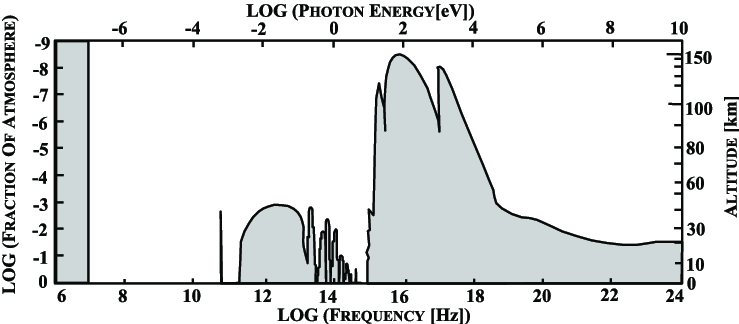
\includegraphics[width=0.7\linewidth]{figures/chapter2/transparency}
    \caption{Altitude above which the atmosphere becomes transparent for different frequecies of electromagnetic radiation. To observe soft X-rays (0.1--10 keV) it is necessary to reach altitudes above 80 km. The steep jump near 1 keV is due to photoelectric effect of nitrogen and oxygen. For hard X-rays (10--100 keV) and $\gamma$-rays ($>100$ keV) the minimum altitudes goes down to about 20--40 km. Image taken from \cite{transparency}.}
    \label{fig:transparency}
\end{figure}

This opportunity allowed to access a new perspective on the universe, which led to the discovery of new types of sources and to a better understanding of the physical processes that take place in astrophysical sources during high-energy events. An example is Scorpius X-1, the first detected extrasolar X-ray source and the most luminous persistent source of the X-ray sky. It has an X-ray luminosity about $10^3$ times larger than its optical counterpart, indicating that the emission processes are very different from those of the Sun, where the X-ray luminosity is about $10^{-6}$ times smaller than the visible light luminosity. Indeed, Scorpius X-1 is a Low Mass X-ray Binary system (LMXB) where a compact object, a neutron star in this case, accretes material from its companion and the emission is mainly due to the conversion of gravitational energy into thermal energy. Many other X-ray sources with various nature were discovered in the following years, such as active galactic nuclei, which are extragalactic sources where a supermassive black hole with a mass larger than $10^6$ M$_{\odot}$ accretes matter from the surrounding environment releasing enormous amounts of energy. All of these high-energy sources are united by the presence of extreme conditions, with gas heated to very high temperatures up to $10^{10}$ K or with high energy particles that interact with matter or magnetic fields producing high energy photons, both in the X and $\gamma$ regions of the electromagnetic spectrum. 

The limiting factor for the detection of X-rays is detector sensitivity. Indeed, the incoming fluxes from astrophysical sources are quite small. For reference, during active phases the Sun can reach a flux of $10^6$ ph cm$^{-2}$ s$^{-1}$ in the range 2-10 keV while Scorpius X-1 has a flux of about 30 ph cm$^{-2}$ s$^{-1}$ and 3C 273, the most luminous AGN, about 0.01 ph cm$^{-2}$ s$^{-1}$. The necessity to improve flux sensitivity, in order to discover fainter sources, has led the research and developement of X-ray detectors, which have evolved substantially across the years and have employed very different technologies.

\section{X-ray observables}

\fix{Qui potrei descrivere le 4 osservabili importanti nell'astrofisica X, che sono energia, imaging, timing e polarimetria. Per ogni osservabile descrivo quali importanti informazioni permette di ottenere (e.g. spettro -> informazioni su meccanimi di emissione, stato della materia, ...). Qualche foto carina di spettri, sorgenti e.g SN / AGN. Per il timing bisogna cercare un po di info, ma si può parlare brevemente delle pulsar in sistemi binari che permettono di effetuare verifiche di relatività generale ma anche di porre limiti alle EOS delle NS grazie alla misura della massa in sistemi binari. Per la polarimetria si può parlare dell'ambiente che circonda le sorgenti, in particolare campo magnetico, e quali info puo dare. Poi si può dare particolare enfasi all'importanza di avere tutte queste informazioni per una singola sorgente, e ancora di piu di effettuare questi studi nello stesso momento grazie a detector che sono capaci di fare piu cose. In particolare per studi di variabilità.}

The four observables that can be measured when a photon is detected are its energy, position, time of arrival and polarization, and each of them allows to understand different aspects of astrophysical sources.

The energy spectrum allows to understand the dominant emission processes of a source which can depend on its physical state, chemical composition and surrounding environment. A high-energy astrophysical source can have thermal or non-thermal emission processes, ...





\section{History of X-ray Astrophysics}
\label{section:history}

The first orbiting satellites to employ instrumentation to observe X-rays were part of the Orbital Solar Observatory (OSO) program, but they were mainly focused on the study of the Sun X-ray emission. Despite their main mission goals, they also performed some observations of galactic and extragalactic sources that allowed to confirm discoveries made by other missions with sub-orbital flights. However, without dedicated instrumentation it was not possible to carry on systematic studies of fainter sources. In this context, a major advancement was achieved with UHURU, the first orbital mission fully dedicated to X-ray observations of extrasolar sources, launched in 1970. Before UHURU, each sub-orbital flight was able to observe the sky for about five minutes, and during the entire 1960s only about an hour of observations was cumulatively gathered. With the launch of UHURU, observations were carried continuosly for over two years, collecting an amount of data many orders of magnitude larger than the entire previous decade. This satellite performed an all-sky survey, scanning a different region of the sky each day. The results allowed to discover more than 300 new sources \cite{4ucatalog}, localized with a precision of 1 arc min, enabling the identification of counterparts in other regions of the electromagnetic spectrum, such as visible and radio.

The heritage of UHURU was collected by the following missions that were part of the high-energy observatories program for X and $\gamma$ astrophysics, the three High Energy Astronomy Observatories (HEAO). One of the most important among them is HEAO-2, known as Einstein Observatory, launched in 1978. Einstein is, strictly speaking, the first true X-ray telescope, meaning that for the first time mirrors were used to focus X-rays onto a detector located in the focal point, marking the birth of imaging X-ray astronomy and paving the way to all the future detectors of this type. Until that moment, an X-ray observatory usually had a set of collimators to mechanically delimit the observed sky region. With different collimator geometries and with dedicated reconstruction algorithms it was possible to achieve a resolution of at most a few arc sec (about $7"$--$10"$ for HEAO-1 \cite{heao1a3}), but still it was not possible to produce images of extended sources. Moreover, a better spatial resolution in a collimator usually implies a decrease of the effective area, with the consequent drop of the signal-to-noise ratio. With Einstein Observatory these problems were solved using focusing optics. However, while for visible light a mirror surface reflects almost all the incoming photons, high-energy photons have a very high probability of penetrating the surface and thus not being reflected. The solution consists in using grazing incidence optics, relying on total reflection of light to have an increase of reflectivity. Indeed, this law holds for X-rays too, with the difference that the total reflection angle is usually below 1 degree and there is a quite strong dependence on the photon energy, making this method feasible only for low energy X-rays up to 10-20 keV. A possible optics geometry is the Wolter, named after its designer Hans Wolter, that consists in using two mirrors to focalize light at low incidence angles, usually one with parabolic section and one with hyperbolic or ellipsoid section. This layout allows to have a field of view large enough to be used in astrophysics and it is one of the reasons that makes it the most common layout between grazing incidence telescopes. The main issue of grazing incidence telescopes is the very small geometrical area due to the small inclination of the mirrors with respect to the optical axis. The natural solution to this problem is to use multiple nested concentrical mirrors to multiply the area, altough it introduces a series of technical and structural problematics that have been overcome in the years thanks to technological improvements. Einstein Observatory employed four nested mirrors with a diameter varying between 33 and 56 cm, a focal lenght of 3.4 m, a geometrical area of about 400 cm$^2$ and the capability of alternating four different detectors on the focal plane. For high resolution imaging, the effective area dropped down to 20 cm$^2$ at 0.25 keV and 5 cm$^2$ at 2 keV, with a spatial resolution of 2 arc sec \cite{heao2}. Other imaging and spectroscopy instruments on board were able to achieve an effective area between 100--200 cm$^2$. Results were remarkable and the first high-resolution images of X-ray sources were produced, allowing to study their morphology in a completely new electromagnetic band, even with a smaller effective area than HEAO-1. This was possible because, contrary to collimator observatories, the entire effective area was focused on a small region of the sky, reducing background signal and consequently increasing the signal-to-noise ratio and the instrumental sensitivity. Einstein Observatory produced a detailed catalogue with almost \num{5000} sources, even observing just a small fraction of the sky. For most of them the localization was accurate enough to identify their optical counterparts.

The successive step in the creation of a new and more populated all-sky catalogue was lead by ROSAT, launched in 1990. ROSAT had an overall design very similar to Einstein Observatory, but the optics layout consisted in larger and more efficient mirrors, that enabled to increase the effective area, and a different focal ratio, in order expand the field of view to faster scan the entire sky. Indeed, ROSAT had a field of view twice as large as Einstein and it also had a more uniform sensitivity across the field of view. In just 6 months, ROSAT was able to observe almost \num{150000} sources \cite{rosat}. During its nine years of operations, ROSAT also studied in detail many different sources, including emission from galactic stars and compact objects, spectral and morphological studies of supernova remnants. For the first time, it was also able to resolve the diffuse extragalactic emission into tens of thousands of AGN, giving a fundamental contribution to the development of the unified model and to variability studies. The limit of ROSAT was its narrow energy range, which was partially attributable to the mirrors geometry, that had a relatively big angle of inclination with respect to the focal axis to achieve a large field of view sacrifying sensitivity to higher energies, but was also due to the detectors employed to reveal X-rays. Indeed, the main imaging detectors types used until ROSAT were Position Sensitive Proportional Counters (PSPC) and Micro-Channel Plates (MCP). PSPC is a gas detector and it looses sensitivity at high energies because the gas becomes optically thin, with a consequent reduction of the quantum efficiency. For similar reasons, MCPs are unefficent at high energies, because X-rays easily penetrate the internal coating and glass. Furthermore, even though MCPs were the only way to achieve very good spatial resolutions, they are not capable to measure photon energy, requiring to alternate different instruments in the focal plane to study morphology and spectrum of a source.

\begin{figure}[htbp]
    \centering
    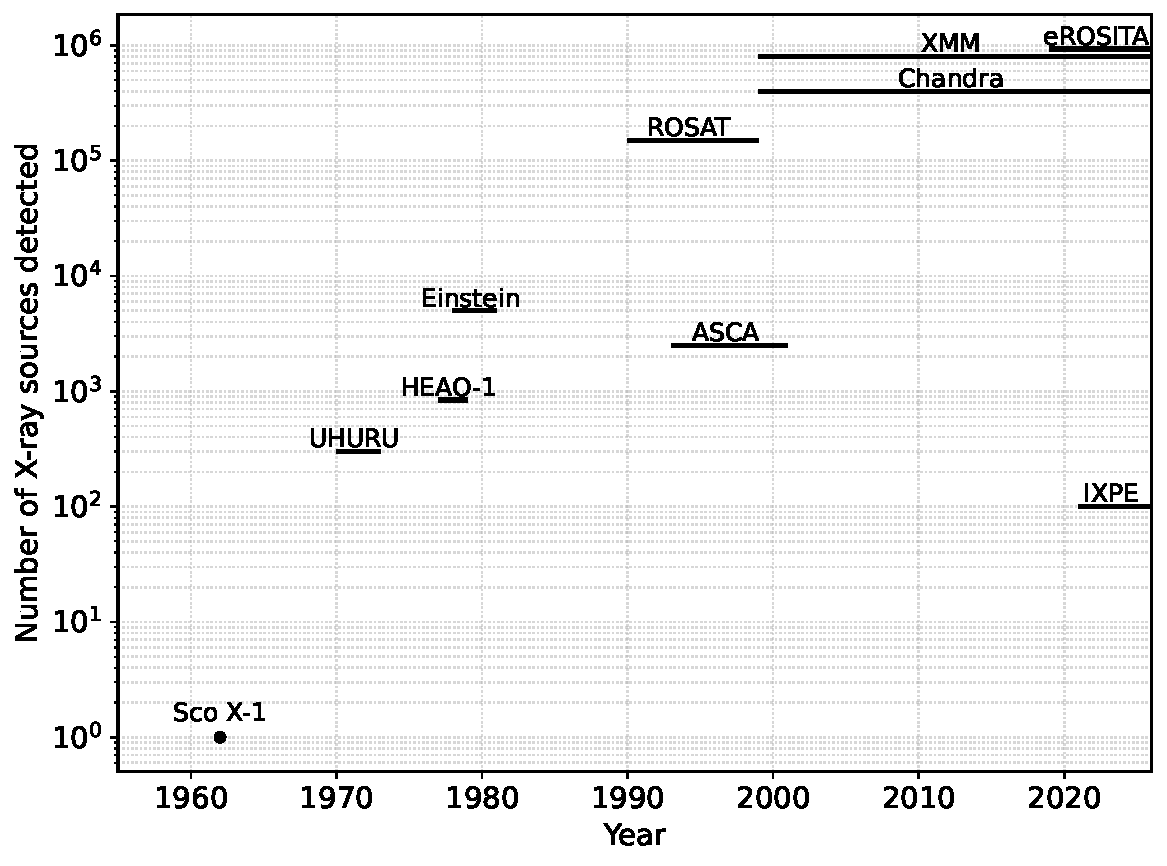
\includegraphics[width=0.7\linewidth]{figures/chapter2/xsources}
    \caption{Number of sources detected by the main X-ray observatories across the years. The horizontal lines represent mission lifetimes.}
    \label{fig:xsources}
\end{figure}


A new mission was launched in 1993 to overcome these limitations, Advanced Satellite for Cosmology and Astrophyisics (ASCA), with two revolutionary changes. The first was in the optics design, that for the first time in a space telescope were realized using a large number of nested concentric metal foils coated with a high-Z metal. ASCA had four telescopes, each with 120 nested gold-coated foils positioned with a very small angle with respect to the optical axis, increasing both the maximum observable energy up to 12 keV and the effective area, which reached 325 cm$^2$ at 1 keV for each telescope (when considering only the optics). The second innovation consisted in the use of CCDs as detectors in the focal plane, the first time for an X-ray telescope. With the use of CCDs in photon counting mode it became possible to perform high resolution imaging and spectroscopy of the source at the same time, even at high energies.

The first generation of X-ray CCDs suffered from various problems, such as low quantum efficiency both at low and high energies, with the latter caused by a small depletion region, and electronical issues were responsible for spectral resolution deterioration. These problems were solved by the following generation of X-ray observatories, with Chandra and XMM-Newton, both launched in 1999 and currently operational. These two missions pushed to the limit the technological advancement of CCDs. XMM-Newton is the first X-ray observatory to employ a high thickness and fully depleted CCD \cite{xmm_pn}, ensurin high quantum efficiency in the entire operational energy range, which reaches 15 keV. On the other hand, Chandra's CCDs were optimized for low energy X-ray photons and spatial resolution, improving the readout electronics to decrease noise and also reducing the pixel size, in order to take full advantage of the 10 meters long focal length and achieve a spatial resolution of $0.5$ arc sec \cite{chandra}. Fig. \ref{fig:sensitivity} shows a measure of the sensitivity of some of the cited observatories by estimating the observed surface source density above a certain flux threshold.

\begin{figure}[htbp]
    \centering
    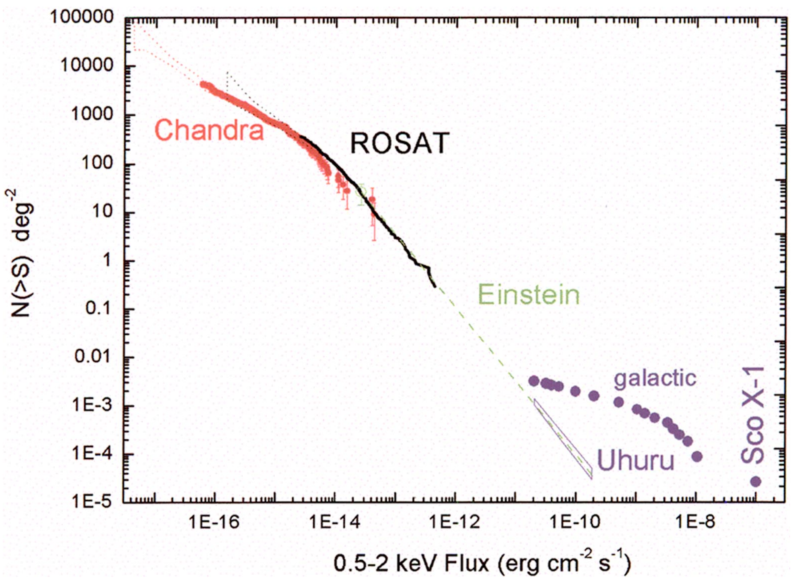
\includegraphics[width=0.7\linewidth]{figures/chapter2/sensitivity}
    \caption{Sensitivity of some X-ray observatories across the years, represented as number of sources with flux above a threshold $S$ observed in a square degree of sky as a function of the flux $S$ between 0.5 and 2 keV. The lower limit for each observatory is an indicator of the minimum observable flux. The slope of the curves is an indicator of how the sources are distributed across the universe. In case of UHURU the slope is different because the majority of sources are galactic, thus they have a different spatial distribution. Image taken from \cite{giacconi2003}.}
    \label{fig:sensitivity}
\end{figure}

Beyond imaging and spectroscopy, polarization of X-ray emission from a source can be studied to infer important properties about its surrounding environment, such as magnetic fields, and the physical mechanisms at play \cite{xray_polarimetry}. The first successful X-ray polarimetry mission took place in 1971 and was carried out with sub-orbital rockets using a crystal Bragg polarimeter, resulting in the first measure of the polarization level of the Crab Nebula. This type of detector consists in a crystal of a specific material, which defines a narrow energy sensitivity band, mounted at an angle of 45 degrees with respect to the incident flux. If a photon has the electric field vector parallel to the crystal surface it is reflected, otherwise it penetrates the crystal and is absorbed. By counting the photons that are reflected as a function of the azimuthal angle while the detector is spinning around the axis that points towards the source, it is possible to measure the level of polarization. For many years this method represented the only feasible way to measure X-ray polarization, but there were many physical and technical problems associated to it. First of all, the energy range is very narrow, thus the observed rate is small and the consequence is that even for bright sources the observation time required to detect polarization is very long. The second big problem is technical, because it is difficult to make the detector spin pointing exactly towards the source, with the possibility of introducing systematics errors that could false the polarization. For these reasons a mission completely oriented to X-ray polarimetry was never realized until a new technique to measure was developed. This new method consists in using the dependence of the direction of motion of primary photoelectrons released in photoelectric absorption on the polarization. Tracking the motion of electrons after absorption allows to reconstruct the initial angle. This is the operational basis of Imaging X-ray Polarimetry Explorer (IXPE), launched in 2021, where Gas Pixel Detectors (GPD) are employed. IXPE allows to reach high sensitivity with observing times at least two orders of magnitude lower than old missions. Another important aspect of IXPE is its ability to provide not only polarization data of the observed source, but also imaging, spectral and timing data at the same time. More details about IXPE and its detectors will be given in Chap. \ref{chap:chapter3}.

\begin{table}[htbp]
\centering
\small
\begin{tabularx}{\textwidth}{l l X c c}
Mission & Lifetime & Main instruments & Energy [keV] & Eff. Area [cm$^2$] \\
\toprule
UHURU 	 & 1970--1973   & Proportional counters & 2--20 & 840 \\
\addlinespace
Einstein & 1978--1981   & PSPC & 0.4--4.0 & 100 \\
         &              & Microchannel plates & 0.15--3.0 & 5--20 \\
\addlinespace
ROSAT	 & 1990--1999   & PSPC & 0.1--2.5 	& 240 \\
         &              & Microchannel plates & 0.1--2.5 & 80 \\
\addlinespace
ASCA 	 & 1993--2001   & CCD	& 0.4--12 & 105 \\
		 &				& Gas scintillation PC & 0.8--12 & 50 \\
\addlinespace
Chandra	 & 1999-- 		& CCD & 0.2--10 & 340 \\
		 & 				& Microchannel plates & 0.1--10 & 225 \\
\addlinespace
XMM 		 & 1999-- 		& CCD MOS & 0.1--15 & 922 \\
		 & 				& CCD PN  & 0.1--15 & 1227 \\
\addlinespace
IXPE		 & 2021-- 		& Gas pixel detector	  & 2--8	  & 167 	  \\

\bottomrule
\end{tabularx}
\caption{Some of the X-ray missions representing the technological evolution of X-ray detectors and telescopes, from collimators to grazing incidence optics and from gas proportional counters to solid state pixel detectors for imaging and spectroscopy and Gas Pixel Detectors for polarimetry.}
\label{tab:missions}
\end{table}


\section{Light-matter interaction mechanisms}
There are three main mechanisms with which high energy photons can interact with matter, which are photoelectric effect, Compton scattering and electron-positron pair production. These processes are at the basis of photon detection and are commonly employed in the construction of high-energy photon detectors \cite{longair1992, leo1994}.

\fix{Forse bisogna inserire qualcosa di generico sulla lunghezza di assorbimento, ma non nel fotoelettrico.}

\subsection{Photoelectric effect}
When a photon has an energy $E_{\gamma} \ll m_e c^2$ the main interaction process is photoelectric effect, which consists in a photon that is absorbed by an atom with the consequent ejection of a free electron

\begin{equation}
\gamma + (A, Z) \rightarrow e^- + (A, Z)^+.
\end{equation}

A photon with energy $E_{\gamma}$ can be absorbed and cause the ejection of an electron only if $E_{\gamma} \geq E_B$, where $E_B$ is the binding energy of the involved electron. The electron is expelled with a kinetic energy equal to $E_{\gamma} - E_B$. The atomic energy level structure can be observed from the appearance of jumps in the photoelectric cross section, which are referred to as absorption edges. Atomic electrons are arranged in shells, with increasing binding energy from the outermost to the innermost one. When a photon has enough energy to interact with a more internal shell, the cross section rapidly increases. In heavy elements with high atomic number $Z$, the large binding energy difference between orbitals inside the same shell is responsible for the apperance of further small edges. The photoelectric cross section usually has a strong dependence on the photon energy and on $Z$, and for the K-shell, corresponding to the innermost $1s$ spherical shell, it scales as

\begin{equation}
\sigma_{K} \propto E_{\gamma}^{-3.5}Z^5.
\end{equation}

Outer shells have a strong dependence on energy and atomic number as well, but it gradually decreases going outwards. Fig. \ref{fig:photo_cross_section} shows photoelectric cross section dependence on energy for silicon ($Z = 14$) and for the compound material cadmium-telluride CdTe, a crystal made by cadmium and tellurium ($Z_{Cd} = 48$, $Z_{Te} = 52$). For both materials is possibe to observe the increases in the cross section corresponding to the K-edge, while for CdTe there is also the L-edge. Because of the large difference between the atomic numbers, CdTe has a cross section almost $10^3$ times larger than silicon for energies above the K-edge at about 30 keV.

Once the photoelectron has been ejected, the atom is in an excited state and there are two major mechansisms with which it can return to the ground state. Generally, an electron from an outer shell fills the vacancy caused by the photoelectric effect and the difference is in the later de-excitation process. The first process consists in the emission of an Auger electron, which happens when the electron that filled the vacancy transfers energy to an electron in the outer shells, causing the ejection of the latter with a kinetic energy that corresponds to almost the entire de-excitation energy. Furthermore, the emission direction is isotropic. The second process is X-ray fluorescence emission, which happens when the energy is released by emitting a photon with energy corresponding to the binding energy difference between the vacancy and the outer electron levels. After this processes, the atom is then left with one or two vacancies in the outer shells that, depending on the state of the material, can be filled by recombination, with consequent emission of low energy photons, or by non-radiative thermal dissipation. The probability of emitting fluorescence radiation instead of an Auger electron, called fluorescence yield, depends on the atomic number and on the shell. Fluorescence yield generally increases with $Z$ and for inner shells, as shown in Fig. \ref{fig:fluorescence_yield}, and it becomes dominant for atoms from $Z \approx 30$.

\begin{figure}[h]
    \centering
    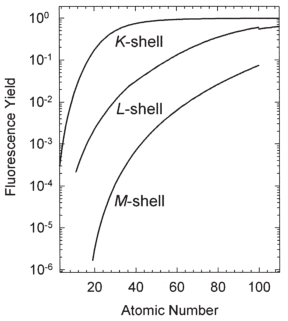
\includegraphics[width=0.45\linewidth]{figures/chapter2/fluorescence_yield}
    \caption{Fluorescence yield for elements $3 \leq Z \leq 110$ for K, L and M shells. Values showed for L and M shells represent the average between subshells. Plot taken from \cite{xraydatabooklet2009}.}
    \label{fig:fluorescence_yield}
\end{figure}

Another important property of photoelectric effect is its dependence on the photon polarization. When considering absorption by spherical shells, the differential cross section is \cite{muleri2008}

\begin{equation}
\frac{d \sigma}{d \Omega} \propto \frac{\sin^2 \theta \cos^2 \phi}{(1 + \beta \cos \theta)^4},
\end{equation}
where $\phi$ is the angle between the polarization vector and the direction of emission of the photoelectron, and $\theta$ is the polar angle, which measures the angle between the incidence direction of the photon and that of emission of the photoelectron. This dependence can be exploited to measure the degree of polarization of a source, which can be inferred by tracking photoelectrons and studying counts distribution as a function of $\phi$, which is equal to

\begin{equation}
N(\phi) = A + B \cos^2(\phi - \phi_0),
\end{equation}
where $A$ and $B$ are the parameteres that describe the degree of polarization. \fix{add other info?}

\subsection{Compton scattering}

\begin{figure}[t]
    \centering
    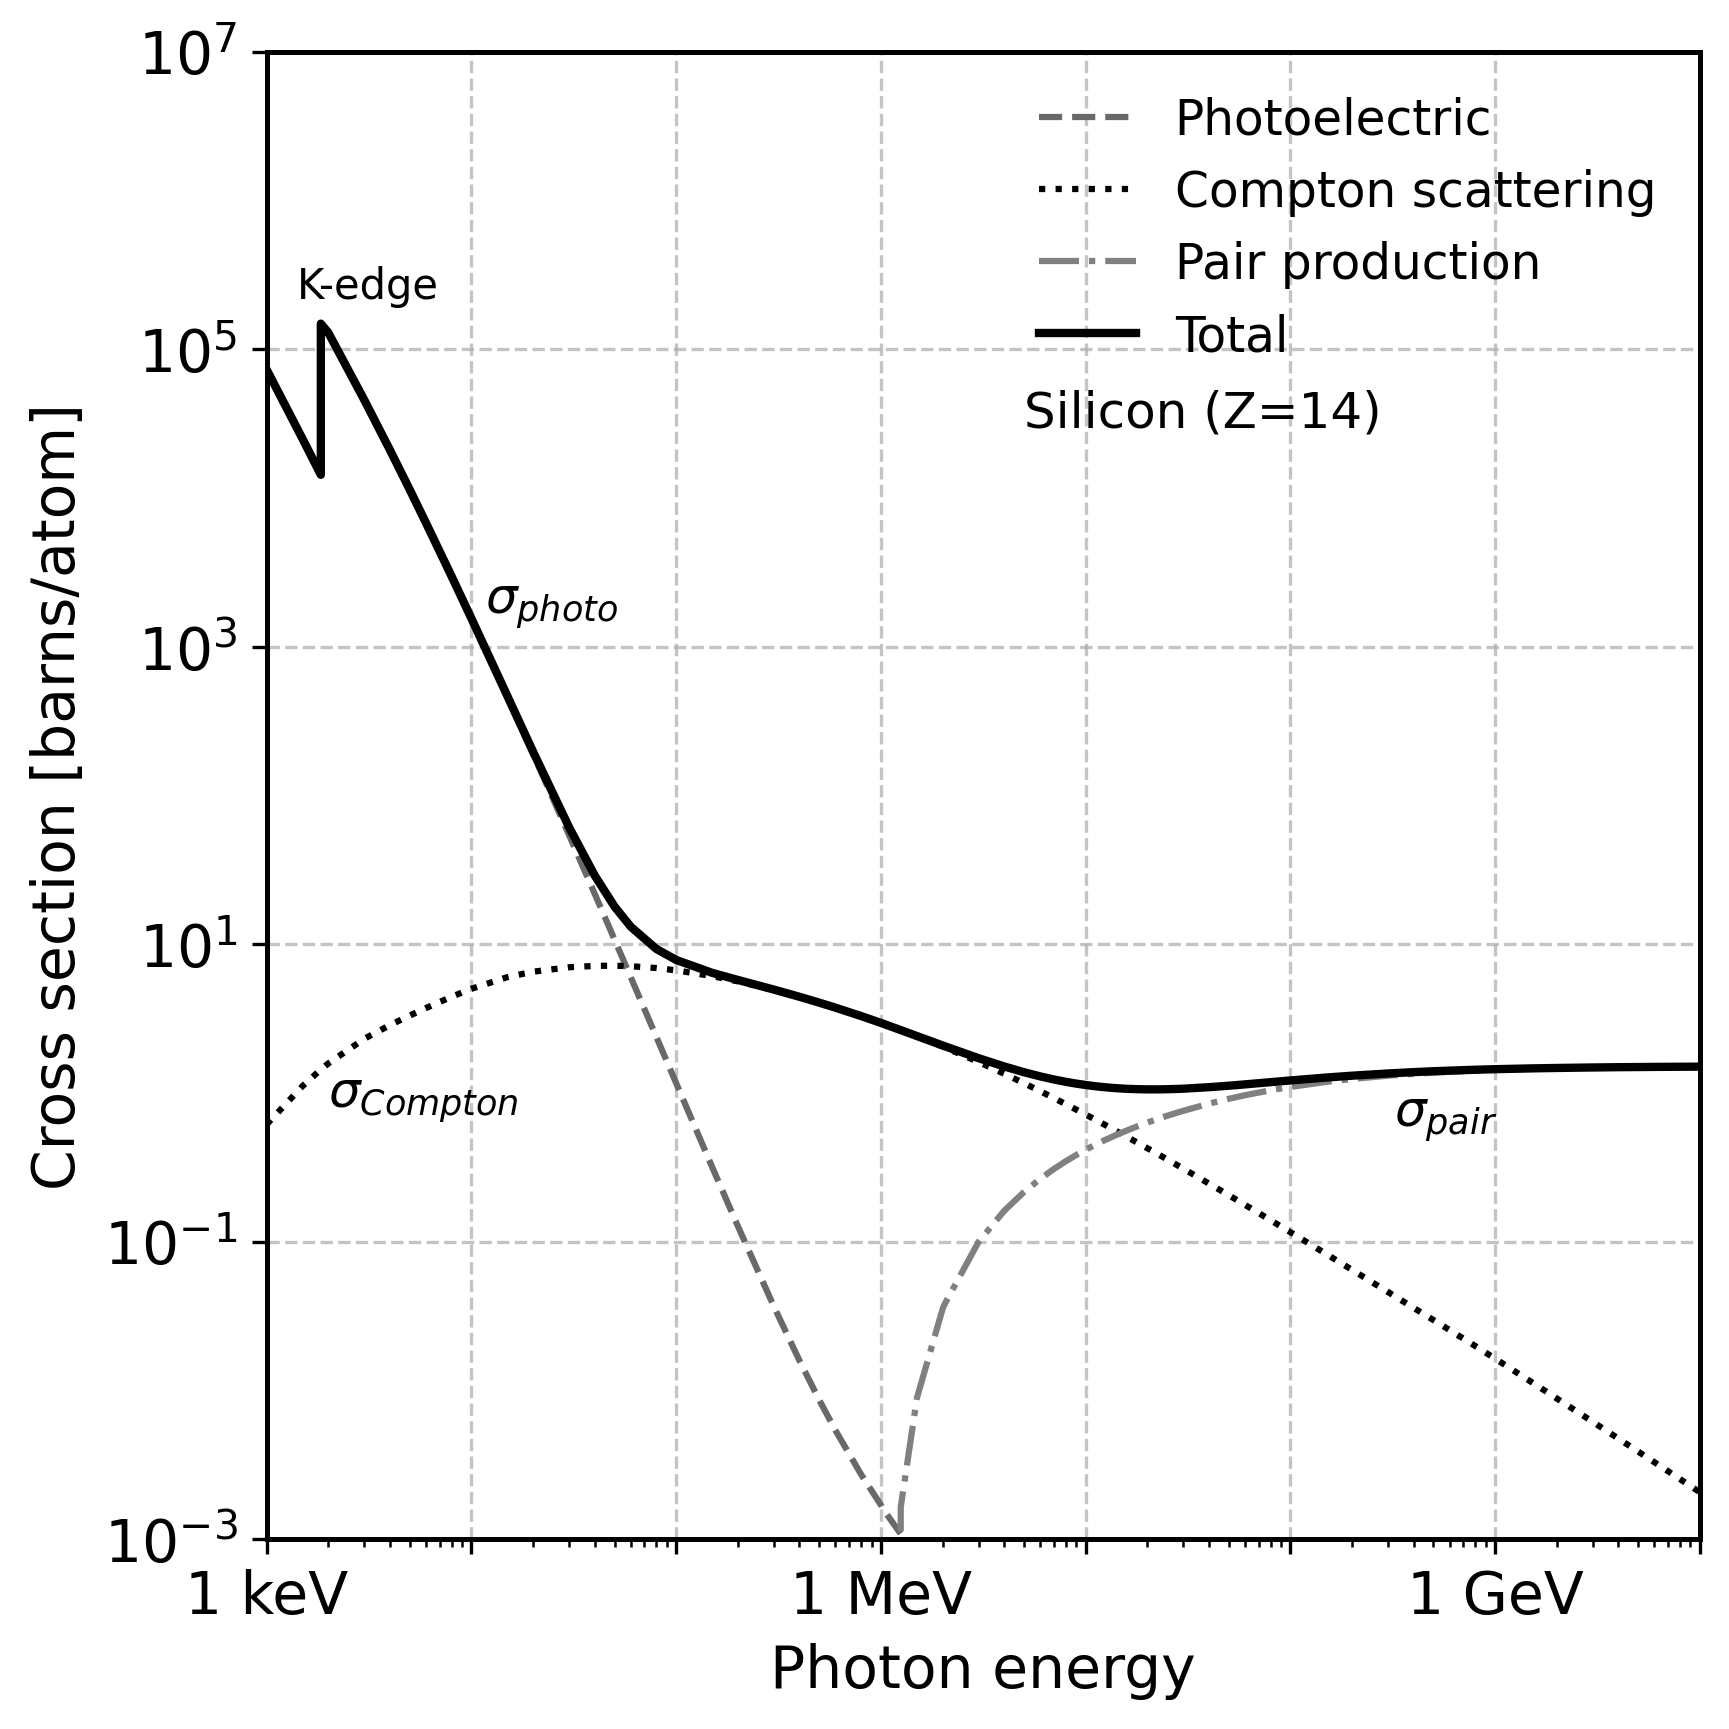
\includegraphics[width=0.49\linewidth]{figures/chapter2/si_cross_section}
    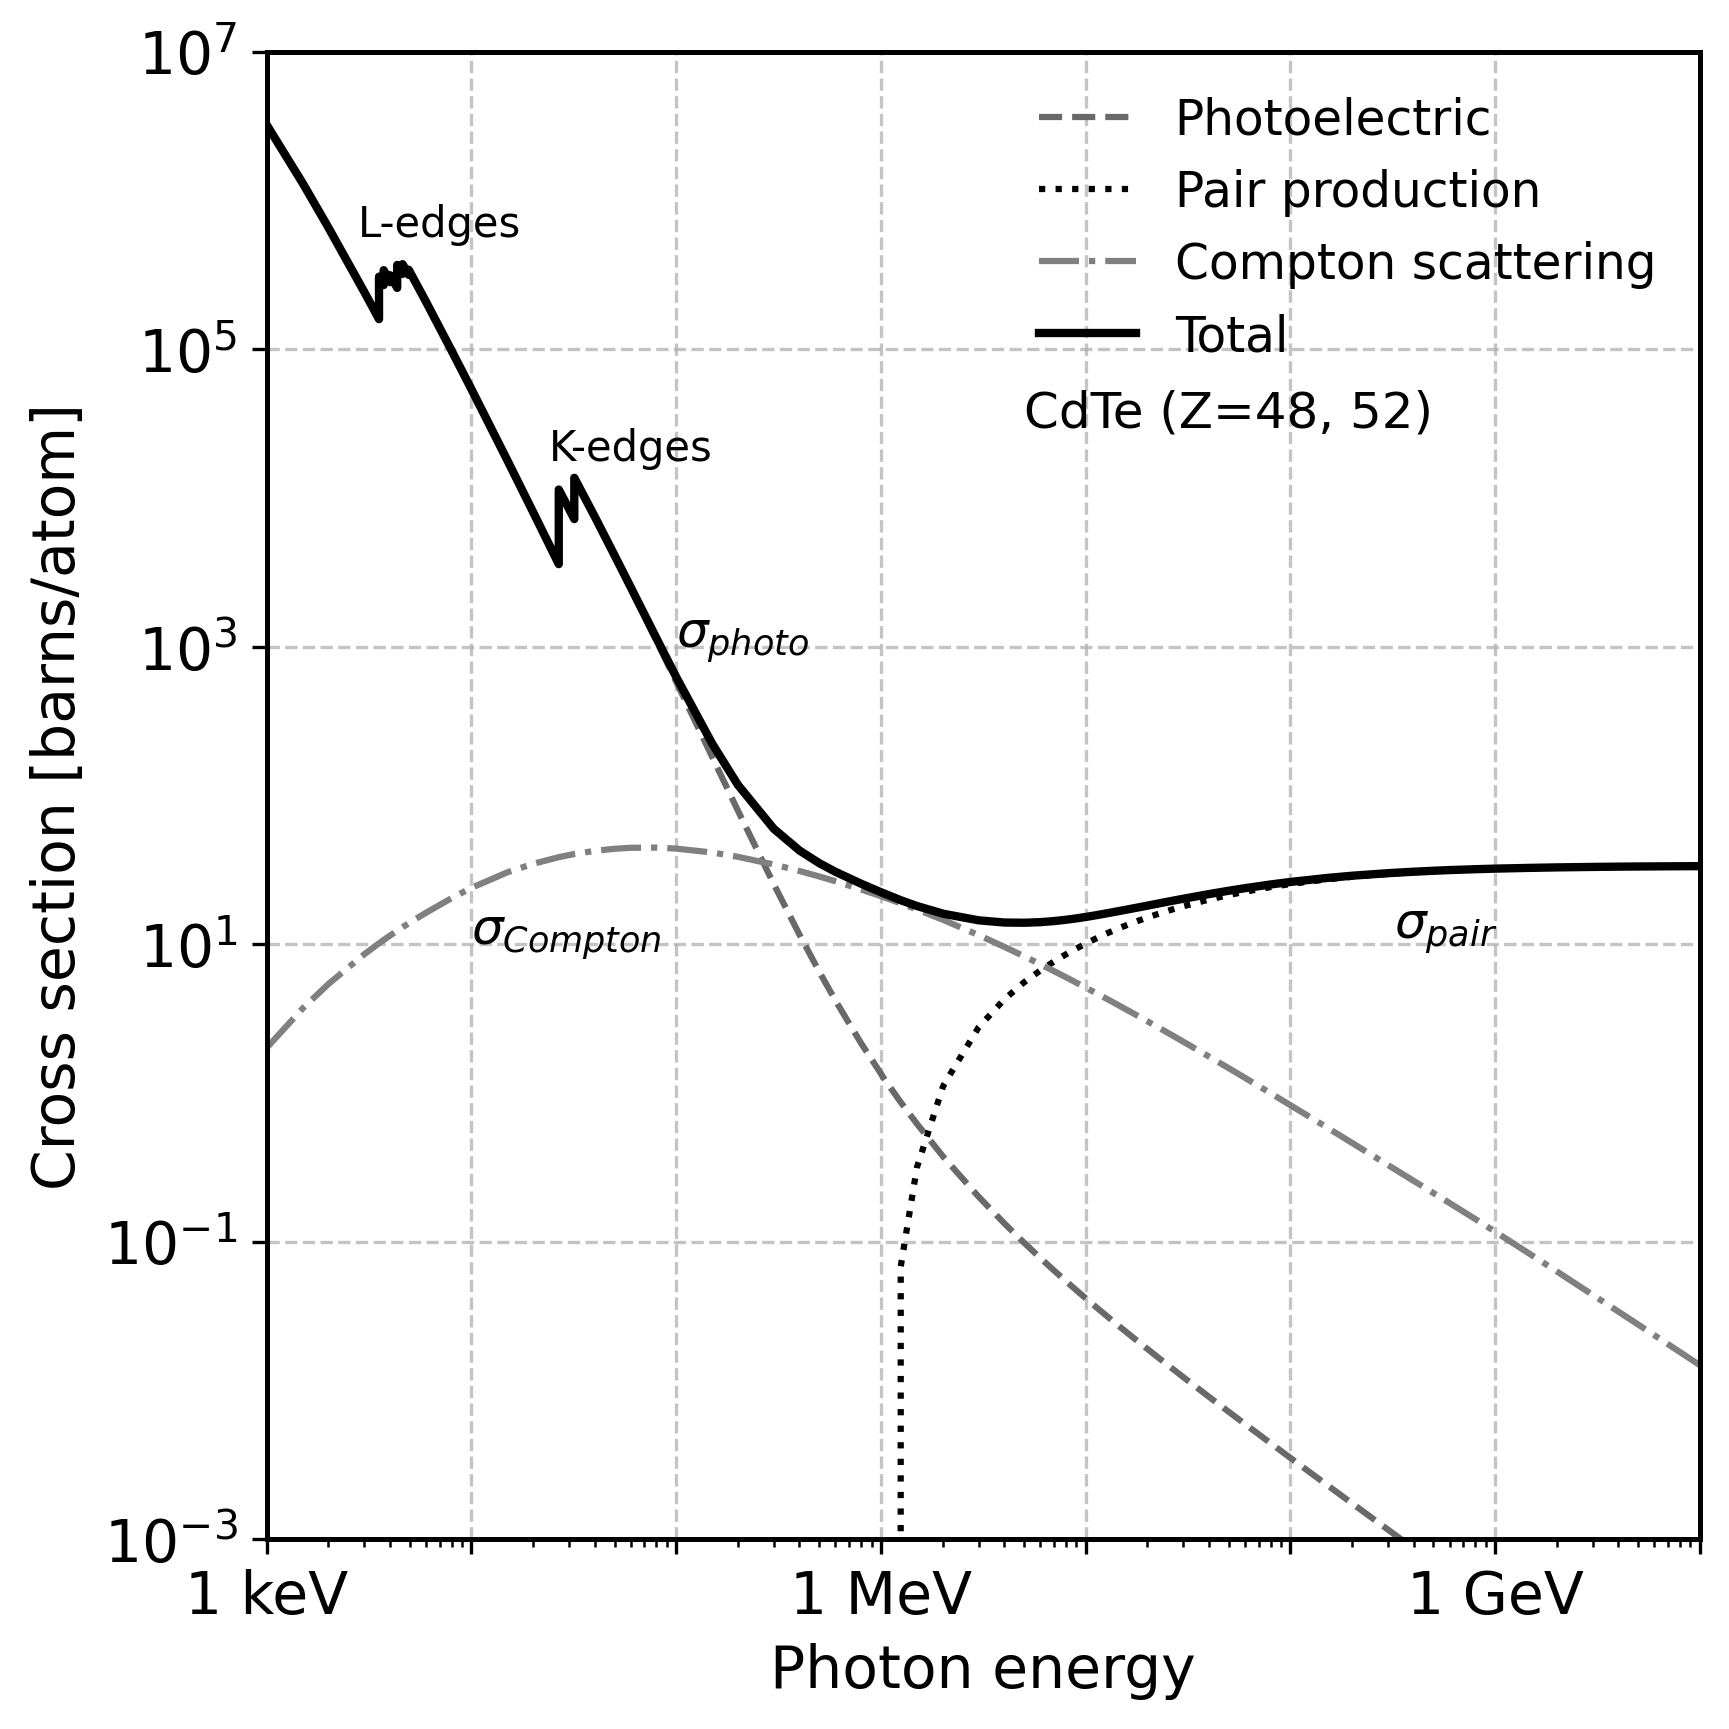
\includegraphics[width=0.49\linewidth]{figures/chapter2/cdte_cross_section}
    \caption{Photoelectric effect, Compton scattering, pair production and total cross sections for silicon (left panel) and cadmium-telluride (right panel). Photoelectric effect is the dominant process for energies up to 50--100 keV. K-edge is visible for silicon and CdTe at 1.8 keV and 27--31 keV, respectevely. L-edges are also visible for CdTe, at an energy of about 4 keV. Compton scattering is dominant from these energies up to 10 MeV, where pair production becomes the prevailing process. Data are gathered from \cite{nist_xcom}.}
    \label{fig:photo_cross_section}
\end{figure}

Compton scattering is the dominant interaction mechanism at higher energies. This process consists in the interaction between a photon and a free electron, with the photon that transfers part of its energy to the electron. It can be represented as

\begin{equation}
\gamma + e^- \rightarrow \gamma + e^- .
\end{equation}

Given the high energy at which the Compton effect becomes relevant, which is much larger than the energy of the K-edge, the assumption that an atomic electron is free and at rest is a good approximation.

In the frame where the electron is at rest, the photon energy after the interaction is

\begin{equation}
E_{\gamma}' = \frac{E_{\gamma}}{1 + \frac{E_{\gamma}}{m_e c^2}(1 - \cos \theta)},
\end{equation}
where $E_{\gamma}$ is the initial energy and $\theta$ is the angle between the photon initial and final directions. The differential cross section for polarized photons is given by the Klein-Nishina formula

\begin{equation}
\frac{d \sigma_{\textrm{C}}}{d \Omega} = \frac{r_e^2}{2} \left( \frac{E_{\gamma}'}{E_{\gamma}} \right)^2 \left( \frac{E_{\gamma}'}{E} + \frac{E_{\gamma}}{E_{\gamma}'} - 2 \sin^2 \theta \cos^2 \phi \right),
\label{eq:compton}
\end{equation}
where $r_e$ is the classical electron radius, $\phi$ is the azimuthal angle measured with respect to the polarization vector and $\theta$ is polar angle. When considering an atom with atomic number $Z$, the total Compton cross section scales as $\sigma_{\textrm{tot}} \propto Z \sigma_{\textrm{C}} $, showing a much weaker dependence on $Z$ compared to photoelectric effect. Fig. \ref{fig:photo_cross_section} shows the total Compton cross sections for silicon and CdTe, compared to other interaction mechanisms cross sections. The interval where the Compton effect is dominant becomes narrower for large atomic numbers. 

As for photoelectric polarimetry, Eq. \ref{eq:compton} is useful to measure polarization for higher energy photons. Indeed, Compton polarimeters are commonly used to study polarimetry in the hard X-ray and soft $\gamma$-ray bands, in the energy range from a few tens of keV up to a few MeV. 

\subsection{Pair production}
For energies above 10 MeV, in the $\gamma$-ray band, the dominant process becomes electron-positron pair production in the nuclear field, represented by

\begin{equation}
\gamma + X \rightarrow X + e^+ + e^- .
\end{equation}

This process can cinematically take place only if the photon has an energy above threshold $E_{\gamma} > 2 m_e c^2$. For an atom with atomic number $Z$, the total cross section scales as 

\begin{equation}
\sigma_{\textrm{pair}} \propto r_e^2 Z^2.
\end{equation}

At low energies, the cross section increases logarithmically with the photon energy, while at high energies it becomes constant, as shown in Fig. \ref{fig:photo_cross_section}, both for silicon and CdTe.

In high energy astrophysics, this process is exploited in pair production telescopes for $\gamma$-rays, where the produced electron and positron are tracked to determine the incoming photon direction and their energy is measured with an electromagnetic calorimeter to gauge the initial photon energy.

\section{Working principles of X-ray detectors}
As said above, photoelectric effect is the dominant interaction process in the X-ray energy band. For this reason, the following discussion is focused on photon detectors that employ this effect to convert an incoming photon into an interpretable signal which allows to measure one or multiple properties among energy, position, time of arrival and polarization.

Various detectors have been devoleped across the years and used on board of X-ray missions, each of them suitable for measuring one or multiple photon properties in a specific energy interval. The technology empolyed in the construction of these detectors can vary a lot but all of them share the same working principles to convert photons in a readable signal. First, photons interact with the active material through photoelectric effect and are absorbed, producing a photoelectron. This electron can have a lot of kinetic energy and it is transfered to the active material by collisions. The amount of energy lost by collisions is described by the Bethe-Bloch formula

\begin{equation}
- \frac{dE}{dx} = 2 \pi N_A r_e^2 m_e c^2 \rho \frac{Z}{A} \frac{1}{\beta^2} \left[ \ln \left( \frac{2 m_e \gamma^2 v^2 W_{\textrm{max}}}{I} \right) - 2\beta^2 \right].
\end{equation}

In ionization detectors, the energy transfered by the photoelectron ionizes atoms and molecules generating a large number of charge carriers, which in turn induce a current during their motion. Alternatively, in scintillators molecules are excited by the photoelectron and the signal is represented by the luminous emission produced by the de-excitation, which then is collected, converted and amplified to generate an readable electric signal.

The focus of this section is to briefly discuss which are the main ionization X-ray detectors and how they work. These detectors can be divided in two macro-groups, gas and solid state detectors, and are more suitable for soft X-rays detection, but can be adapted to detect hard X-rays as well by varying materials and working points. Hard X and soft $\gamma$ rays detection was dominated by scintillation detectors in the past, but in the last two decades solid state ionization detectors made with high-$Z$ materials have increasingly replaced them. 

\subsection{Gas ionization detectors}
The first X-rays detectors to be launched in space were gas detectors, thanks to decades of experience and development in ground-based experiments and to their low weight, which is essential to launch a satellite in orbit. A gas detector generally consists in a closed chamber filled with pressurized gas. A photon interacts with the gas and the photoelectron ionize it, generating a certain number of free electrons and ions. The number of electron-ion pairs produced after the interaction with a photon is stochastic and depends on the energy and the gas properties. The mean number of electron-ion pairs can be calculated as

\begin{equation}
N = \frac{E}{w},
\end{equation}
where $w$ is a quantity specific to a material and represents the mean energy necessary to create a pair. For gases this value ranges between 20 and 40 eV. As a first approximation, the number of pairs is distributed according to a Poisson distribution, thus the variance is given by the mean number of pairs produced. However, if all the incoming energy is absorbed by the gas, as is the case of X-ray photons, an additional constraint is added, because the number of pairs that are produced and the energy required to generate them is fixed by the photon energy. This means that pair production events are not independent, thus the Poisson distribution approximation is no longer valid. Under these hypotheses the variance is

\begin{equation}
\sigma^2 = F N,
\label{eq:fano}
\end{equation}
where $F$ is called Fano factor. Tab. \ref{tab:w_fano} shows the mean ionization energy and Fano factor for some common materials used for ionization detectors. For most of materials, including gases and semiconductors, $F < 1$. Therefore, when the amount of deposited energy is fixed, the variance is smaller. The energy resolution of the detector can be estimated with the assumption that for a large number of events the number of pairs is distributed according to a Gaussian distribution with the variance obtained from \ref{eq:fano}. The relative energy resolution at the energy $E$ is defined as
 
\begin{equation}
\frac{\Delta E}{E} = \frac{\operatorname{FWHM}}{E} = 2.35 \frac{\sqrt{F N}}{N} = 2.35 \sqrt{\frac{F w}{E}}.
\end{equation} 

The final energy resolution is the sum of more contributes, as other sources of uncertainties must be taken into account, such as electronic noise and all the other possible instrumental noise sources.

\begin{table}[htbp]
\centering
\small
\begin{tabularx}{\textwidth}{X c c}
Material & Mean energy for pair creation [eV] & Fano factor \\
\toprule
Argon &  & \\
Xenon &  & \\
Silicon & & \\
Cadmium-telluride &  & \\
\bottomrule
\end{tabularx}
\caption{Mean energy for pair creation and Fano factor values for various gases and semiconductors. \fix{fillare la tabella, che altri materiali posso mettere?}}
\label{tab:w_fano}
\end{table}

In gas, only a few hundreds electron-ion pairs are produced after the interaction of a photon with an energy of a few keV. Furthermore, pairs are produced in a small and localized region, and without an external field that separate them they would recombine before it would be possible to detect the signal. These are the reason why gas-ionization detectors usually have a drift region and a multiplication region, both employing an external electric field to separate or accelerate charges.

In the drift region, an electric field of the order of 1 kV/cm is responsible for the separation of electron-ion pairs to avoid recombination. Charges are accelerated under the work of the electric field, which is generated applying a potential difference between electrodes. The geometry of electrodes can significantly vary between different detectors, with some examples represented by the axial geometry of cylindrical proportional counters or planar geometry. Inside the drift region charges are subjected to diffusion processes due to collisions and thermal agitation. If no external field is present along an axis, charges are distributed according to a Gaussian distribution, with standard deviation equal to

\begin{equation}
\sigma = \sqrt{2D t_d},
\end{equation}
where $D$ is the diffusion coefficient, which depends on the material and on the working conditions (such as pressure or temperature), and $t_d$ is the drift time, which depends on the charge carriers mass and on the applied electric field. This holds along each axis where an external field is not applied.

The multiplication region is where charges are multiplied and it is achieved by accelerating charges with a strong electric field, with typical peak values of the order of 100 kV/cm. The kinetic energy is used by the charges to start an avalanche by further ionizing the gas, producing new electron-ion pairs that are accelerated by the electric field and in turn continue to ionize the gas. The induced current produced by the charges generates an amplified signal that exceeds electronic noise and can be read and processed. Depending on the voltage applied to the electrodes and the resulting intensity of the electric field, charge multiplication has different working regimes. At low voltages no multiplication process takes place and pair recombination is the dominant process. At higher voltages recombination is not favored, and in a certain interval multiplication occurs and the number of final electron-ion pairs is proportional to the number of primary ionization pairs. The ratio between the initial and final number of pairs represents the gain of the detector. This property is essential for spectroscopy, as it is possible to reconstruct the photon energy. In this voltage interval, which is called proportional counting region, gain grows exponentially with the voltage

\begin{equation}
G = e^{a V}.
\end{equation}
When the voltage becomes too high, the response becomes non-linear and even few ionization events produces a large pulse. This regime is called Geiger-Muller region. Detectors working in this regime are able to detect radiation but can not 

Charge multiplication can be obtained with various designs, going from electrodes disposed as in a cylindrical proportional counter to more complex and miniaturized designs, such as in micro-strip gas chambers or two-dimensional patterns like Gas Electron Multipliers (GEM).

The detector that flew on board of the first dedicated orbital mission, UHURU, consisted in a set of proportional counters. The external part of a proportional counter is usually a thick metallic case, which serves as the cathode, with thin windows of beryllium or plastic material that allow to suppress photons with energies below a few keV. The anode is a thin metallic wire positioned in the middle and running along the long axis. A voltage is applied to the anode to generate an electric field with an intensity that scales ar $1/r$, where $r$ is the distance from the wire. This dependence allows to use the same electrodes to generate the electric field in the drift zone, in a large region far frome the wire, and only when electrons are near the anode they are accelerated to high energies and produce the avalanche. Due to their small mass, electrons reach the anode too fast, thus is the drift of positive ions to generate a detectable signal. In the case of UHURU, all the proportional counters on board were connected in parallel to a single amplifier, thus it had no intrinsic position resolution. The reasons to have multiple proportional counters were essentially for redundancy, in case some of them would have been damaged, and to implement a veto logic to reject signals from cosmic rays.

Indeed, a thing that can not be neglected in space is that the rate of cosmic rays is much larger than that from all X-ray sources. This represents a major source of noise that exceeds the interesting signal. In order to suppress it, a fundamental part that every X-ray detector must have is an anti-coincidence shield, sensitive to cosmic rays and transparent for X-rays, that surrounds the detector and allows to reject a signal when radiation penetrates the entire detector.

To access position information, proportional counters have been gradually improved. Position Sensitive Proportional Counters (PSPC) are one of the improved design and they have the possibility to reconstruct the incidence position of a photon and its energy. This is achieved by using two separated layers of electrodes as cathodes instead of the metallic case. Each layer is a grid of thin spaced wires oriented orhogonally with respect to the other layer. Using this geometry, one layer gives information on the $x$ position and one on the $y$ position. Usually multiple wires were grouped into virtual strips by connecting them in parallel to a single charge pre-amplifier. The anode is made of parallel wires placed in the middle between the two cathodes. A possible layout is shown in Fig. \ref{fig:pspc}. Position resolution is increased thanks to charge diffusion that takes place inside the gas and spreads the charge over multiple strips on both cathodes. Using a simple charge barycenter algorithm it is possible to achieve sub-strip resolution.

\begin{figure}[t]
    \centering
    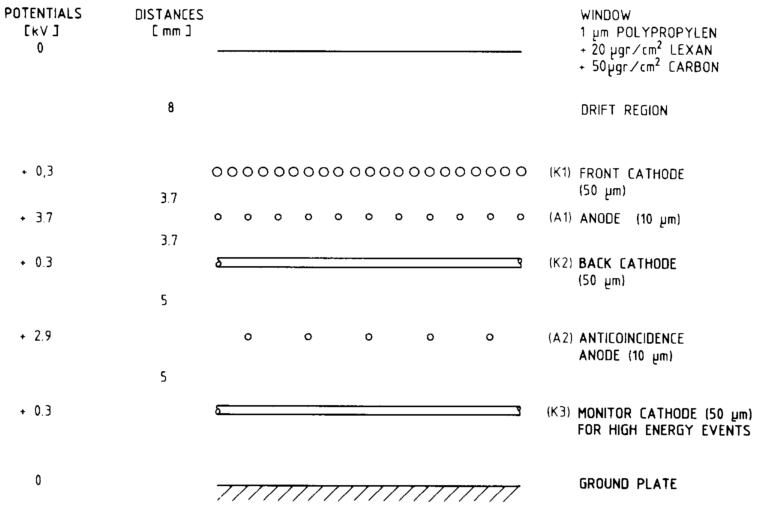
\includegraphics[width=0.7\linewidth]{figures/chapter2/rosat_pspc}
    \caption{Schematic diagram of the ROSAT PSPC \cite{rosat_pspc}. An X-ray photon enters the window and produces a photoelectron by interacting with the gas in the drift region. The photoelectron produces primary ionization electrons that drift to the front cathode and diffuse, creating a large charge cloud that involves multiple strips. These charges are accelerated by the strong electric field between the front cathode and the anode and generate ions that are collected by the front and the back cathode, giving information on the $x$ and $y$ positions. The electrodes after the back cathode are used for anticoincidence logic to reject cosmic rays.}
    \label{fig:pspc}
\end{figure}

Across the years these technologies has not evolved much in X-ray astrophysics and its use has gradually  decreased, in favor of other choices like semiconductors. In recent missions, gas detectors were mainly chosen for to cover large detection area for cost and technical reasons. \fix{devo parlare di qualcosa inerente a IXPE qui oppure rinviamo tutto a capitolo 3?}

 




















\subsection{Solid state detectors}

\fix{qui descriviamo il funzionamento di un detector a semiconduttore, con le varie proprietà, e descriviamo anche il funzionamento delle giunzioni, in particolare pn e schottky. parliamo anche della diffusione della carica all'interno del sensore.}
\fix{The interaction must occur inside the depletion region, but if we are with a fully depleted sensor we don't mind about this detail, because it is always the case}


















\chapter{The heritage of IXPE}
\label{chap:chapter3}

Imaging X-ray Polarimetry Explorer (IXPE) \cite{weisskopf2021} is a mission launched in 2021 by NASA and ASI to study polarization of bright X-ray sources, capable of doing imaging, spectroscopy and timing measurements as well. IXPE is the first mission ever entirely dedicated to soft X-ray polarimetry, and it has a sensitivity more than an order of magnitude higher than Bragg crystal polarimeters used on board of older missions.

This large increase in sensitivity was achievable thanks to the innovations brought by the Gas Pixel Detectors (GPD) \cite{baldini2021}, the class of detectors used on board of IXPE. GPD use photoelectric effect to infer the degree of polarization of a source, in particular they exploit the dependence of the emission angle of the photoelectron on the photon polarization. By collecting enough photons it is possible to measure the polarization of the source by studying the distribution of events as a function of the emission angle.

As of 2026, IXPE is still carrying on observational campaigns, even though the nominal lifetime is only two years. In five years of operations IXPE has observed and measured the polarization of about 100 sources. 

IXPE consists of three identical and independent X-ray telescopes. Each telescope has its grazing incidence mirrors with Wolter-1 configuration and a focal length of 4 m. The mirrors are made of 24 concentric and nested foils of nickel and cobalt, and the layout is optimized for high sensitivity in the range 2--8 keV.

\begin{figure}[!b]
    \centering
    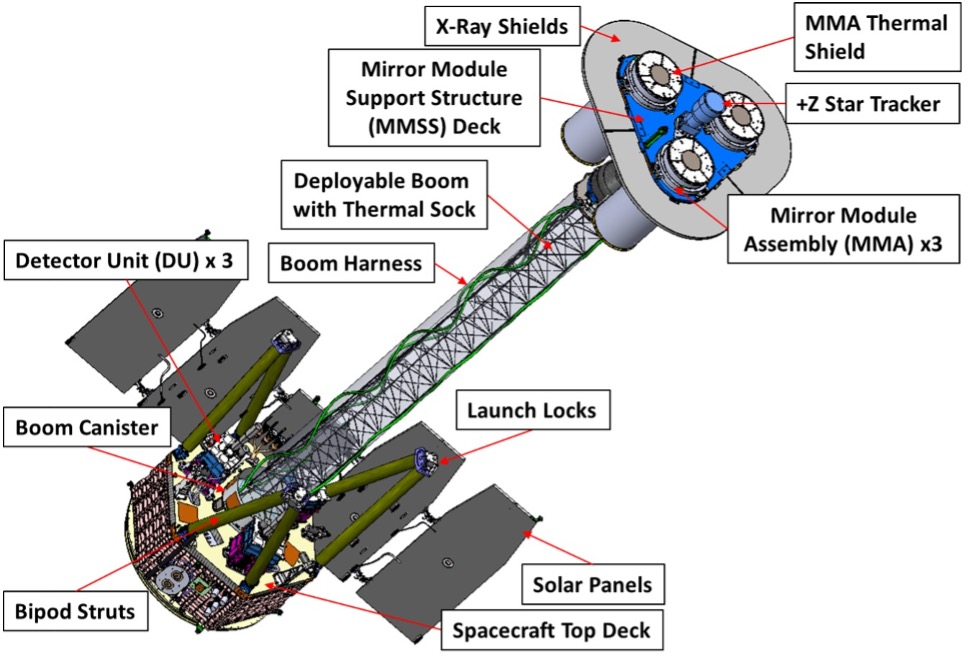
\includegraphics[width=0.6\linewidth]{figures/chapter3/ixpe}
    \caption{Schematic of the IXPE Observatory. Photons enter through the three Mirror Module Assemblies and are collcted by the Detector Units, where GPDs are located. Images courtesy of NASA.}
    \label{fig:ixpe}
\end{figure}

A detector unit (DU) is located on the focal plane of each telescope. A detector unit has a GPD to absorb and analyze X-ray photons, providing position, energy, timing and polarization information.


\section{Gas Pixel Detector}

At the basis of the operations of a GPD is the dependence of the photoelectron emission direction on the incident photon polarization, described by Eq. \ref{eq:polarization_photo}. Photons enter the active gas volume after passing through a beryllium window and can be absorbed. The primary ionization electrons produced by the photoelectron are drifted toward the GEM, which multiply the charges preserving the track shape. The charges generated after the multiplication stage are collected by the pixelated readout ASIC. A schematic example of the GPD and a track are shown in Fig. \ref{fig:gpd}.

\begin{figure}[!b]
    \centering
    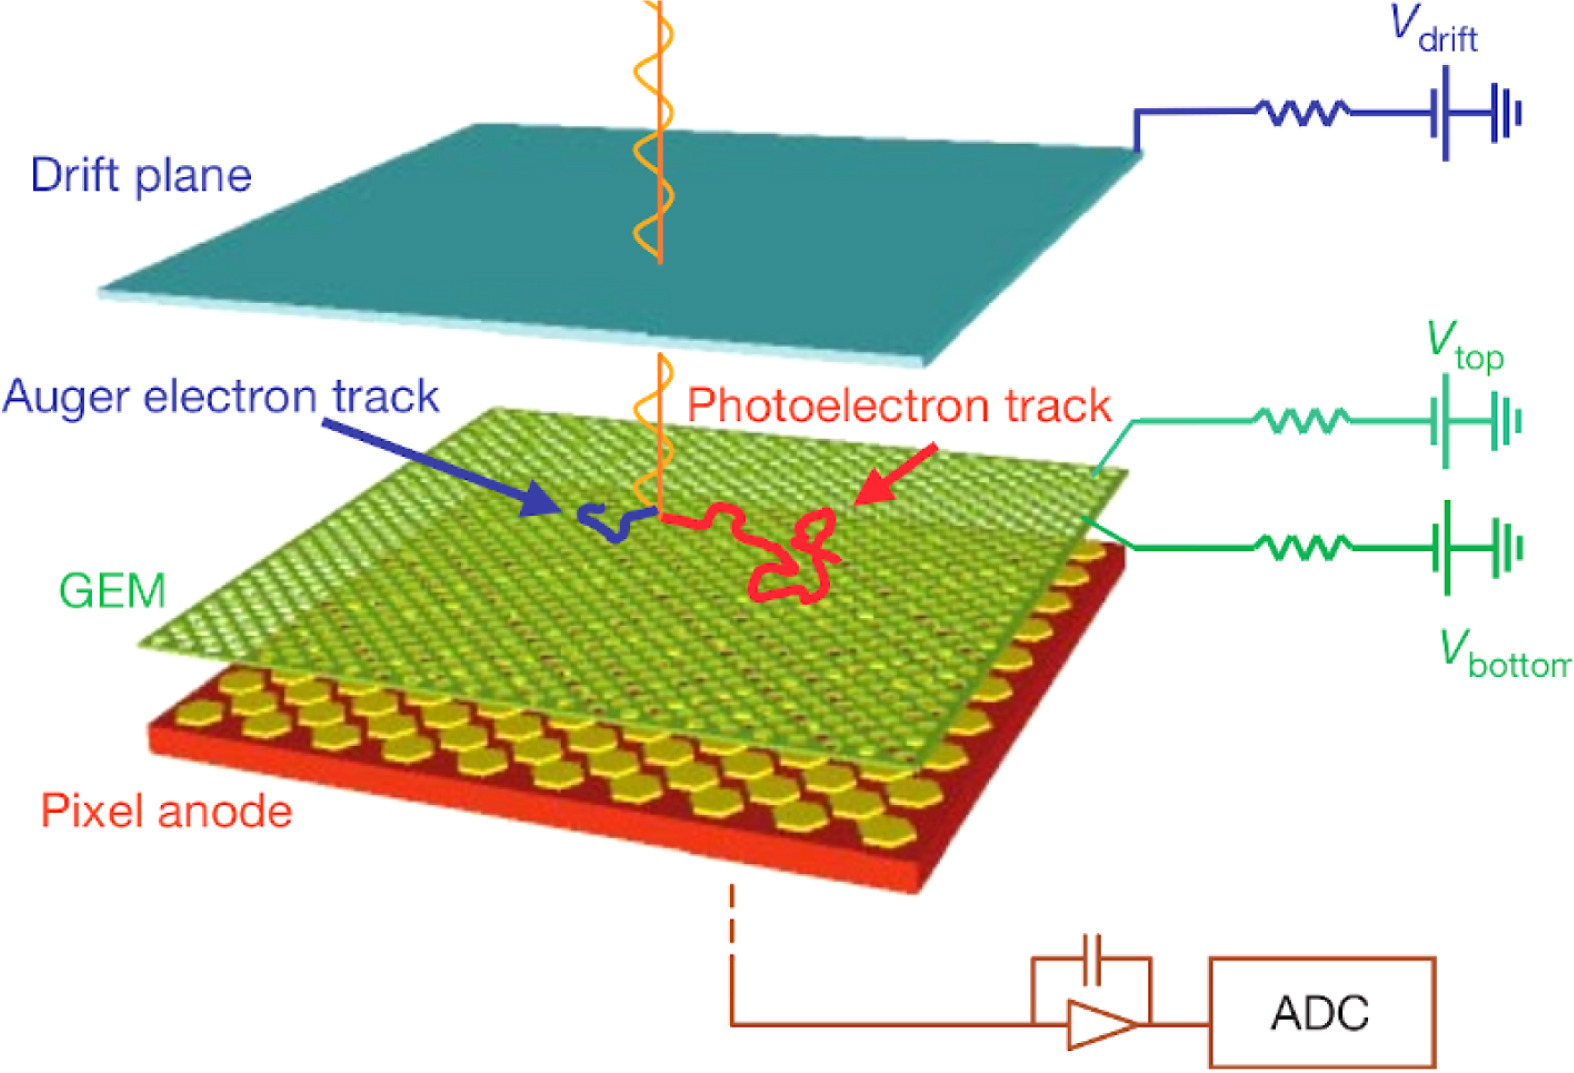
\includegraphics[width=0.49\linewidth]{figures/chapter3/gpd}
    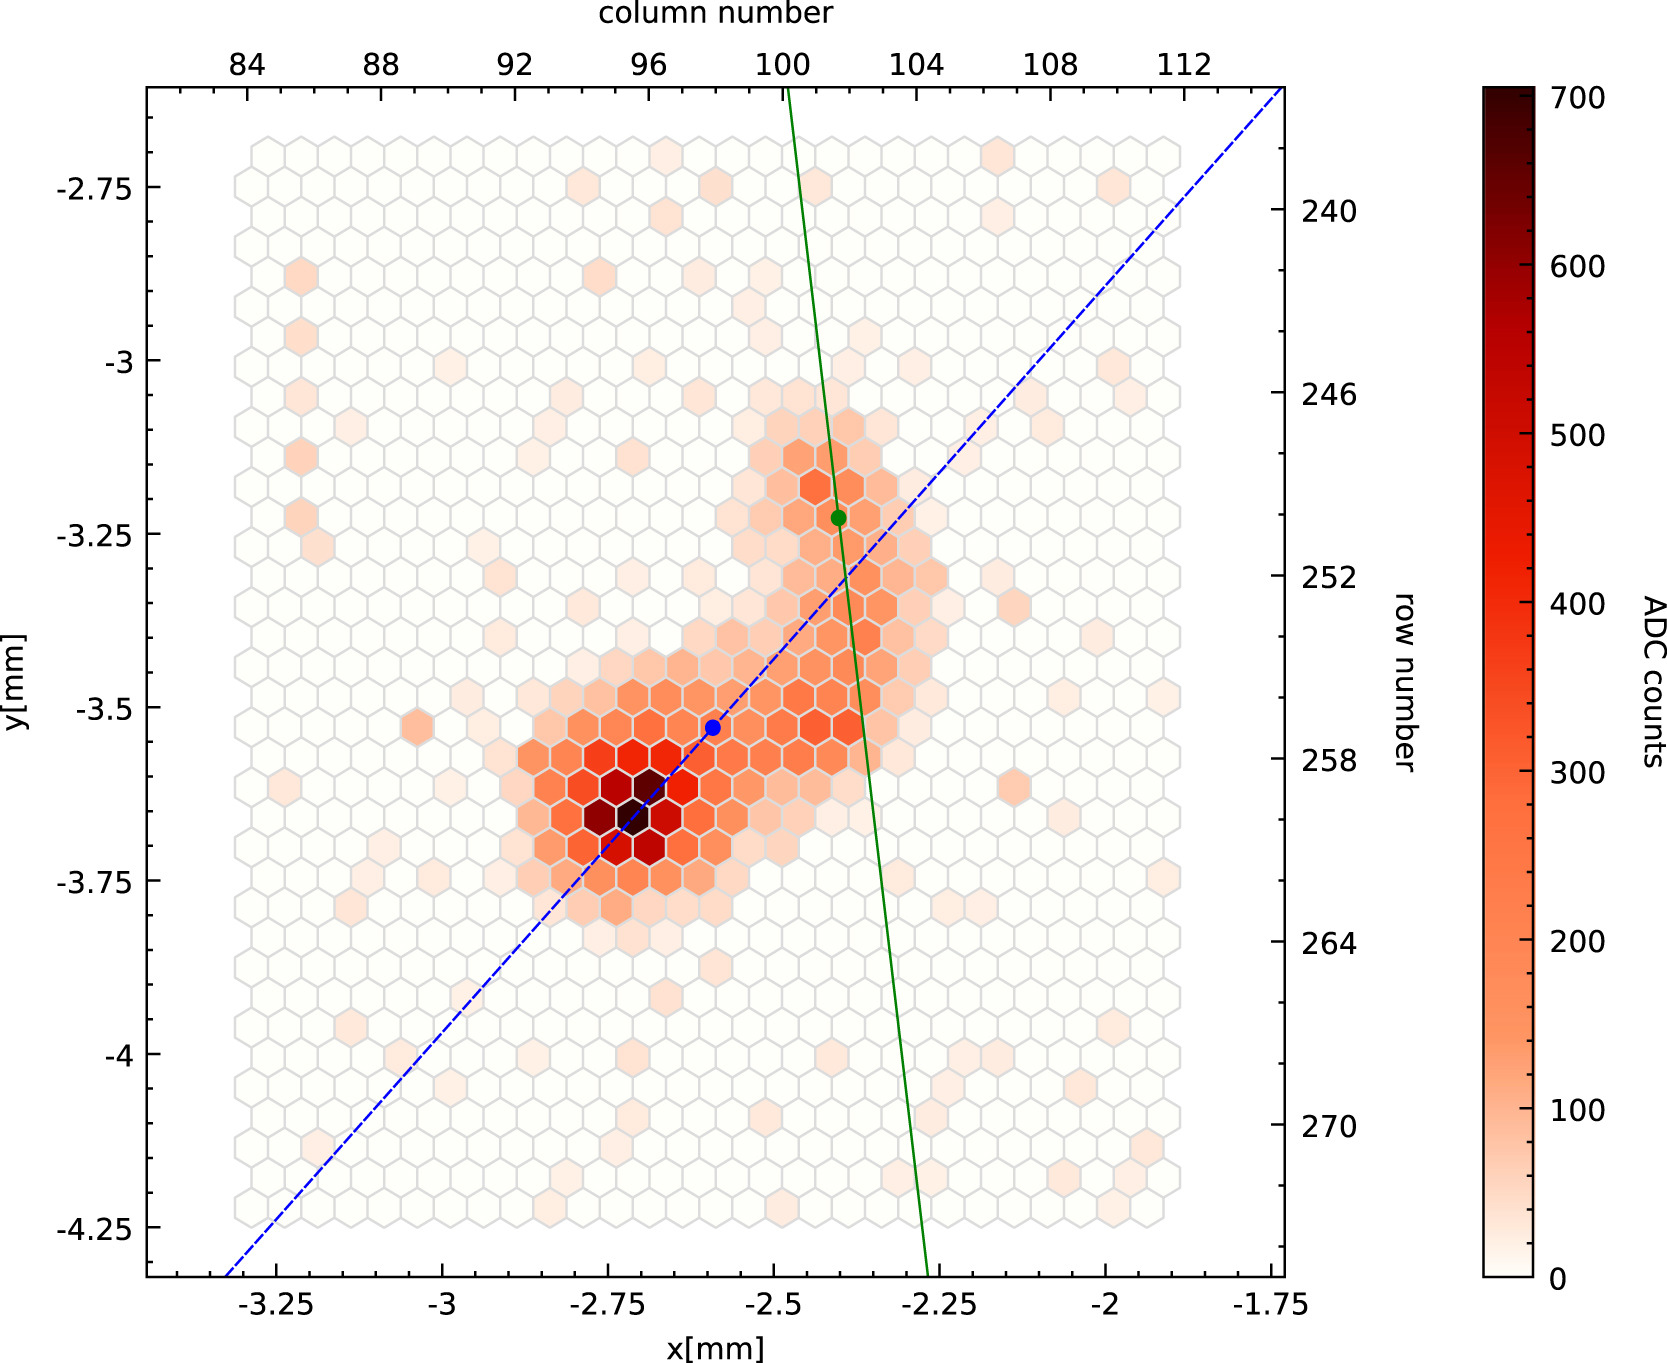
\includegraphics[width=0.49\linewidth]{figures/chapter3/track}
    \caption{The left panel shows the design of the GPD. A photon is aboserbed by the gas volume, producing a photoelectron which is drifted toward the GEM. The produced track is used to reconstruct the photoelectron emission direction. The signal is amplified by the GEM and is read with the dedicated pixelated readout ASIC. The right panel shows an example of a real track from a 5.9 keV photon. Images taken from \cite{baldini2021}.}
    \label{fig:gpd}
\end{figure}

\subsection{Gas cell}
The GPD active gas volume consists of pure dimethyl-ether (DME). The choice of using this gas was made because in order to work as a polarimeter it has to satisfy different requirements. The first is that a light-gas mixture enables to produce long and straight tracks, allowing for a higher efficiency in the polarization level estimate than what is achievable with high-$Z$ gas.

On the other hand, employing a gas mixture with low-$Z$ elements reduces the detector quantum efficiency.  However, there is another constraint which limits the maximum $Z$ that can be used, which is the $K$-edge energy. Indeed, the modulation described by Eq. \ref{eq:polarization_photo} holds only for absorption by spherical shells, thus it is fundamental that the $K$-edge energy is below the design sensitivity range of 2--8 keV.

DME therefore represents a good compromise to satisfy the design requirements. Furthermore, it is usually employed as a quencher, thus it is optimal to avoid accidental discharges in the detector that could compromise its functionalities.

A final important property of DME is that its transverse diffusion coefficient is low, about 68 $\mu$m cm$^{-\frac{1}{2}}$ with an electric field of 2 kV/cm, much lower than other typical gas mixtures (see Fig. \ref{fig:diffusion} for some examples), enabling to limit the track blurring, which represents a limiting factor in the reconstruction of the photoelectron emission direction.

\subsection{GEM}
The GEM \cite{sauli1997} represents the amplification stage of the GPD. A GEM usually consists of a 50 $\mu$m thick Kapton foil with a copper coating on both sides. The GEM is then etched to create holes, which can be tens of micrometers wide. A voltage difference is applied to the copper coatings on the two opposite faces of the GEM to generate a strong electric field inside the holes, as shown in Fig. \ref{fig:gem}.

\begin{figure}
    \centering
    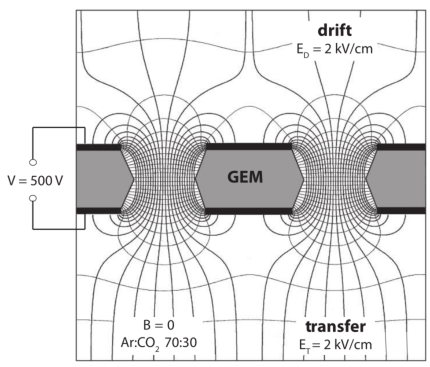
\includegraphics[width=0.49\linewidth]{figures/chapter3/gem_field}
    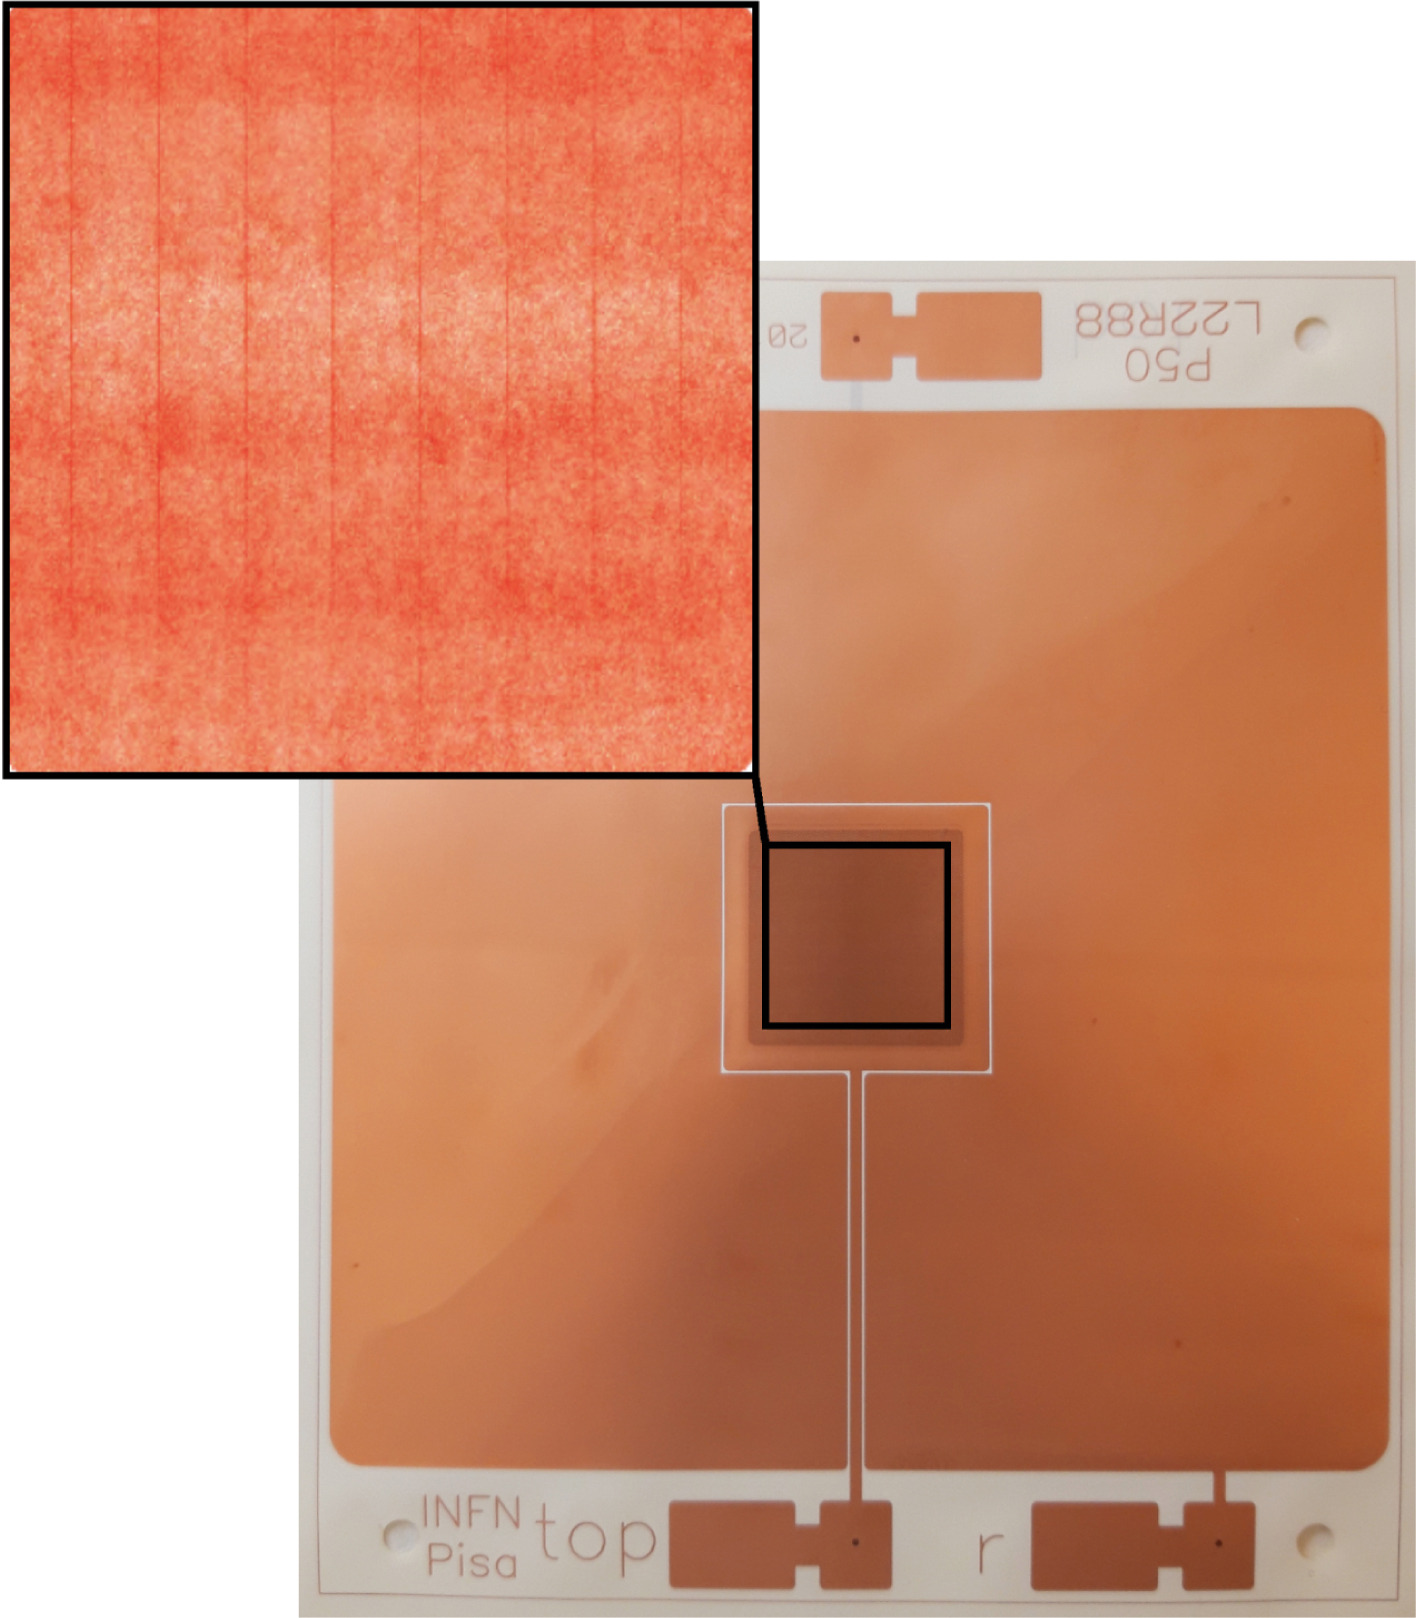
\includegraphics[width=0.4\linewidth]{figures/chapter3/gem}
    \caption{Electric field produced by GEM holes (left panel) when applying a voltage difference between the two copper electrodes (taken from \cite{kolanosky2020}). Photograph of a GPD GEM (right panel), with the darker region representing the active area of the GEM (taken from \cite{baldini2021}).}
    \label{fig:gem}
\end{figure}

The GEM employed inside the GPD is made of liquid crystal polymers (LPC) instead of Kapton, and holes have diameter of 30 $\mu$m. The hole pattern follows a hexagonal grid which matches the ASIC pixel pattern. The GPD GEM is shown in Fig. \ref{fig:gem}, and it is possible to observe the presence of eight equally spaced vertical lines. These lines are a result of the production process, which includes a step where the holes inside the LPC are made through laser drilling. The laser beam has a width smaller than the active region, and it needs multiple sweeps to complete the entire area.

The production process of the GEM directly affects the GPD performances. In particular, it introduces spatially dependent spurious modulations, as shown in Fig. \ref{fig:spurious_mod}. The real cause behind this systematic effect is not known, but one hypothesis is that GEM holes pitch can very along one direction.

In principle this systematic effect could be corrected by taking multiple acquisitions similar to that of Fig. \ref{fig:spurios_mod} by varying the source energy and for each GPD. However, the statistical accuracy required to correct this effect would have required to spend a prohibitive amount of time acquiring data for each detector. Instead of applying a direct correction, the solution adopted to mitigate this effect consists of exploiting the observatory dithering.

\begin{figure}
    \centering
    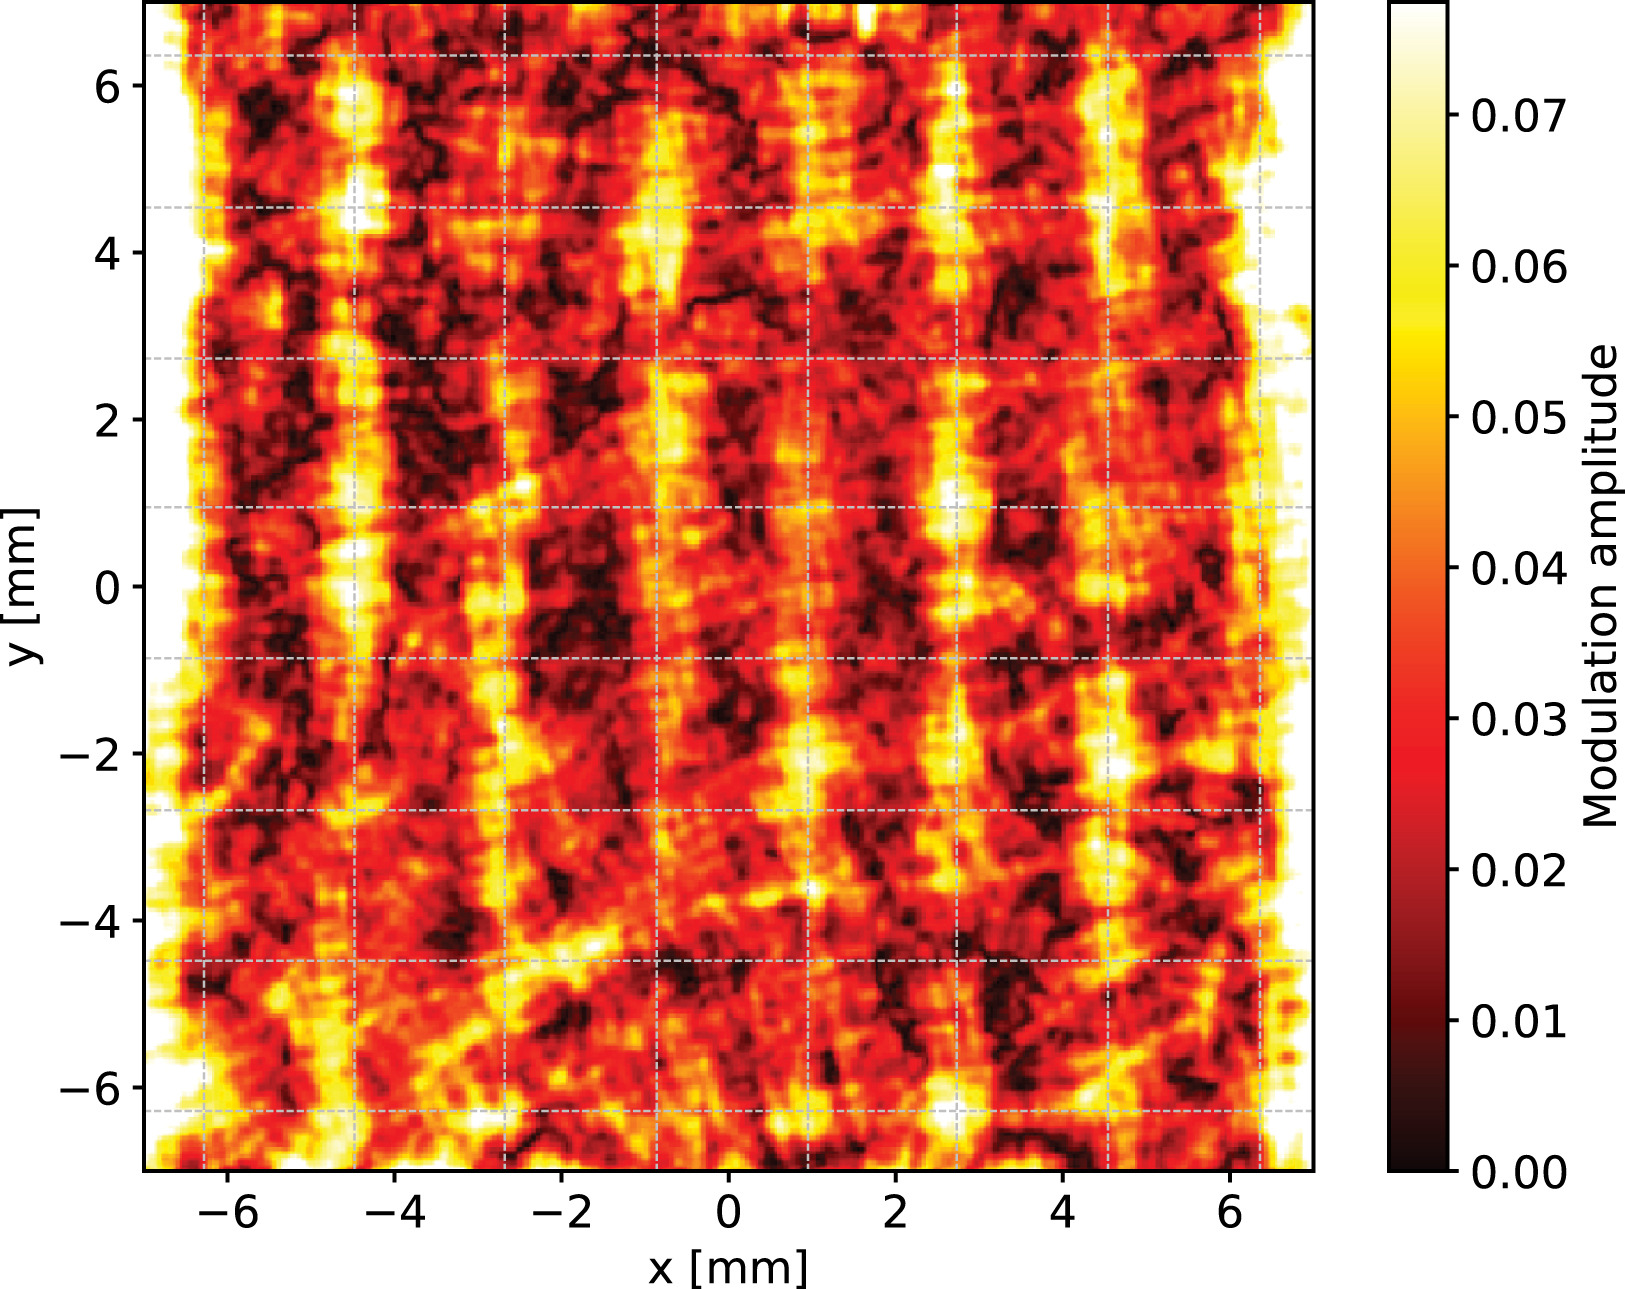
\includegraphics[width=0.49\linewidth]{figures/chapter3/spurious_mod}
    \caption{Modulation amplitude map obtained from an un-polarize X-ray source at 2.7 keV. The dashed gray grid correspond to the coordinates of the laser sweep overlaps (visible in Fig. \ref{fig:gem}) during the GEM production, and it perfectly overlaps with the regions with high-spurios modulation. Image taken from \cite{baldini2021}.}
    \label{fig:spurious_mod}
\end{figure}

Another important effect that depends on the GEM is rate-dependent gain variations. When the detector is operating and is irradiated by a source, part of the charge that is produced by the avalanche inside the GEM holes is temporarily deposited onto the dielectric substrate. This charging phenomenon has the effect of modifying the electric field configuration, with a consequent decrease of the gain.

When the detector is constantly illuminated by a fixed rate source, the gain does not decrease indefinitely but reaches a saturation level after which the gain is approximately constant. The asymptotic gain value and time scale of the process depend on the input energy flux.

This charging effect is reversible because the charge trapping on the dielectric substrate is not permanent. This phenomenon, which consists of a discharging of the dielectric, is a competing process of charging and is continuosly at play, but on much longer time scales. When the incoming flux is sufficiently low, discharging dominates over charging and the gain increases.

In general charging and discharging can be described as rate-dependent, and an example of these processes at play for GPD is shown in Fig. \ref{fig:rate_gain}.

\begin{figure}
    \centering
    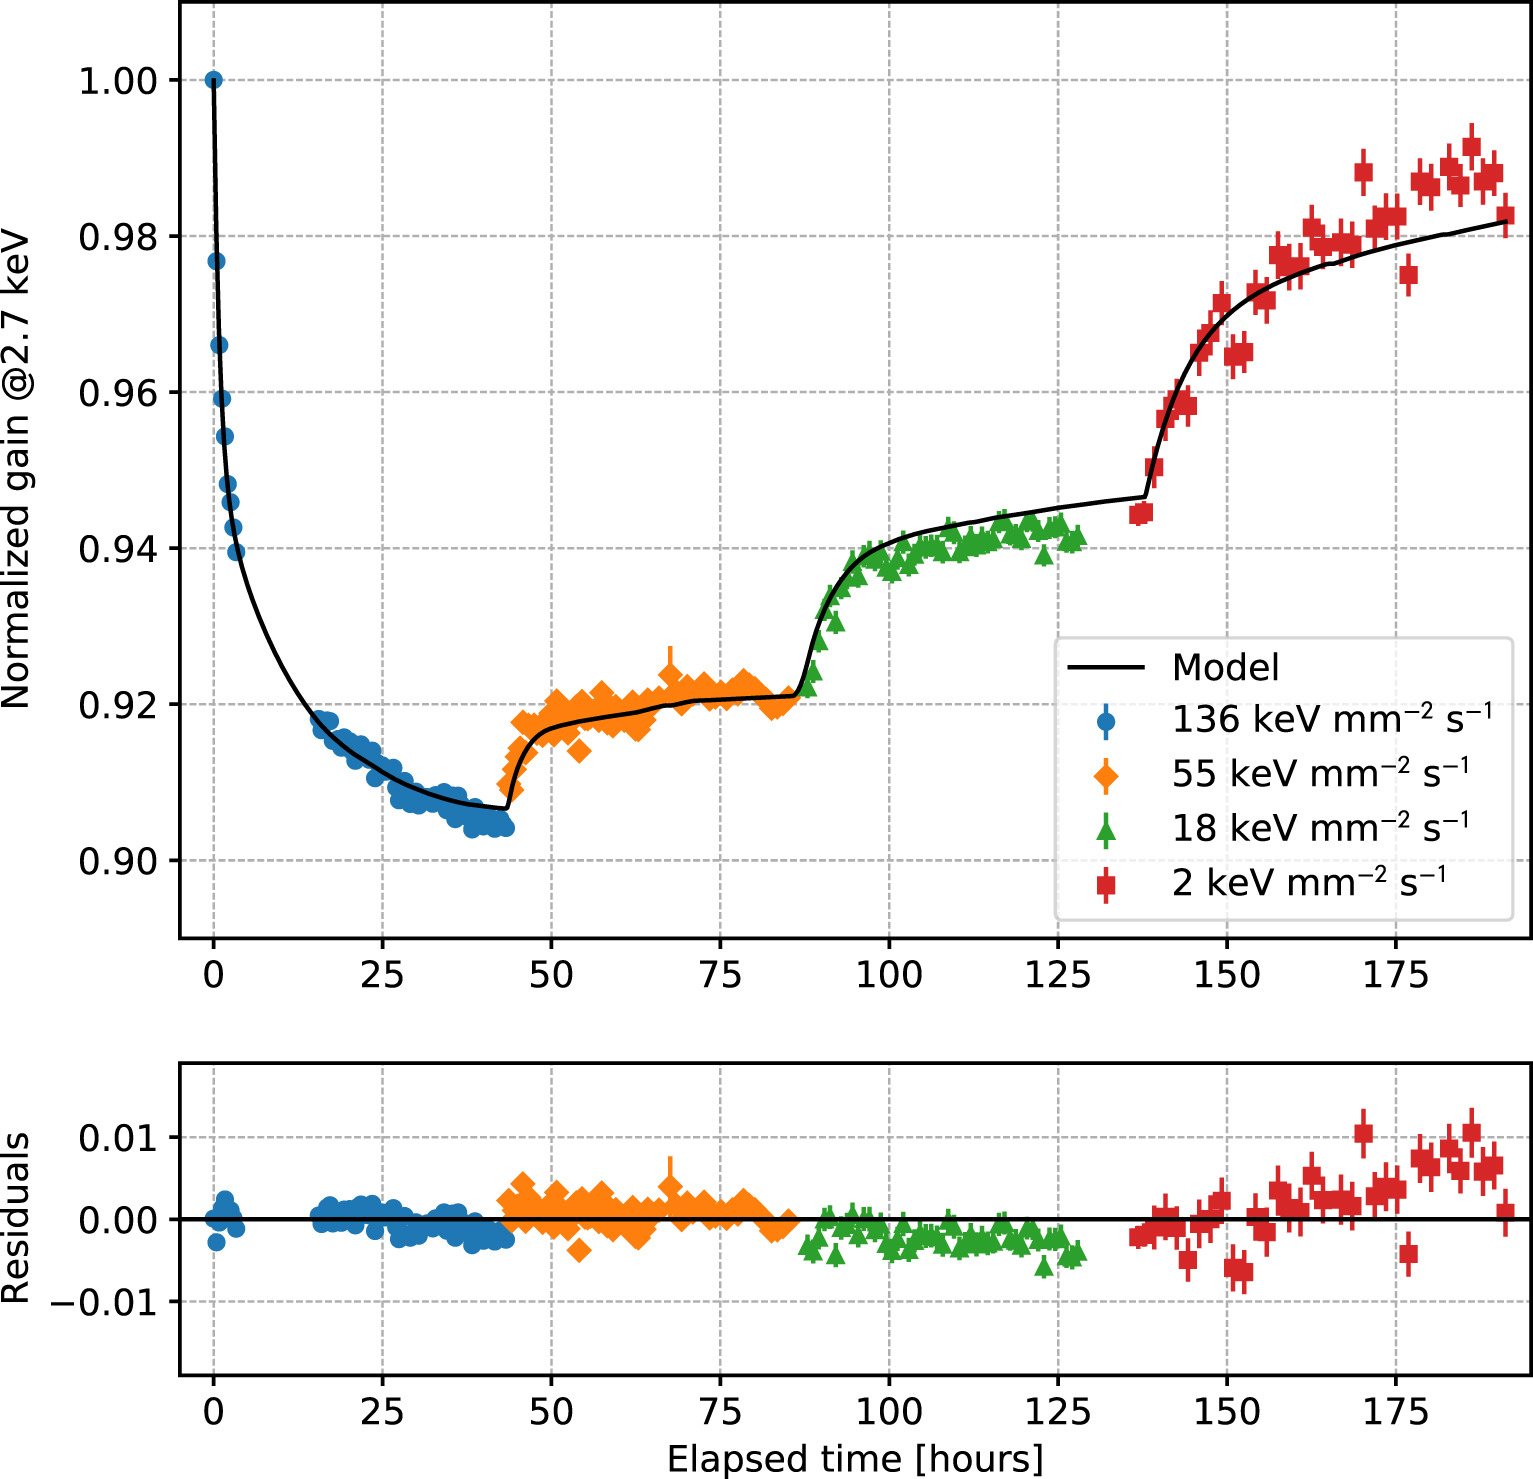
\includegraphics[width=0.49\linewidth]{figures/chapter3/rate_gain}
    \caption{Charging and discharging effects as a function of time for GPD. The different colors data points represent gain measurements taken with different input energy fluxes. First the charging is dominant with a high-flux source which causes almost 10\% of gain decrease. Then, the gain gradually recovers when using lower flux sources.}
    \label{fig:rate_gain}
\end{figure}

These gain variations can be modeled using phenomenological models and can be applied to correct observations. However, limiting the charging and reducing the gain variations amplitude can improve the detector sensitivity to polarization.

Reducing systematic effects, such as spurious modulation and gain variations, which have been observed with this type of GEM is the goal for the next generation of GPD, which is currently under study. One of the alternative which is being developed, which aims on reducing these effects, will be presented in Chap. \ref{chap:chapter5}.


\subsection{XPOL-I ASIC}

\cite{bellazzini2004, bellazzini2006}




\section{XPOL-III}


\label{sec:xpol3}
\cite{minuti2023}

\chapter{Analog Spectral Imager for X-rays}
\label{chap:chapter4}

The Analog Spectral Imager for X-rays (ASIX) is a project which aims to develop a new class of solid-state Hybrid Pixel Detectors (HPDs) capable of performing single photon event-driven readout, designed for both imaging and spectral study of photons at X-ray energies between 1 keV and 50 keV. Contrary to GPDs, these detectors are intended for applications which require energy-resolved imaging different from polarimetry, such as other fields of X-ray astrophysics or material science.

An example of application in material science is X-ray Diffraction analysis (XRD), which is one of the most common nondestructive techniques that provides information about crystallographic structure of a material, its chemical composition and relevant physical properties. Currently, the detectors employed in this field have good spatial resolution, but they have limited energy resolution. A detector capable of selecting photons in a narrow energy band would allow to reduce unwanted background that deteriorates measurements.

The idea behind ASIX is to use the experience gained over the years in the development of the XPOL-family ASICs to test a new design where an XPOL chip is coupled to a solid state sensor. While proving the validity of the sensor design using the recently developed XPOL-III, a new dedicated ASIC is being developed to match the requirements needed in terms of event readout time.

This section illustrates the design and the current state of the prototypes and the dedicated simulation and analysis software that is being employed to evaluate different design concepts and to test the goodness of the detector calibration and analysis pipeline. Furthermore, in the context of the event analysis, different algorithms to reconstruct the position and energy of the photons have been developed and tested using both Monte Carlo simulations and laboratory data, in order to determine their performance.

\section{Detector design}
\label{sec:asix_design}

ASIX is a solid-state HPD and it consists of two main components: the pixelated semiconductor active sensor, which is responsible for the absorption of X-ray photons and the production of electron-hole pairs, and the analog readout ASIC, which processes the collected charge by amplifying and shaping the signal and then triggers the digital readout electronics to save the events. A schematic of the detector with its housing is shown in Fig. \ref{fig:detector}.

\begin{figure}[h]
    \centering
    	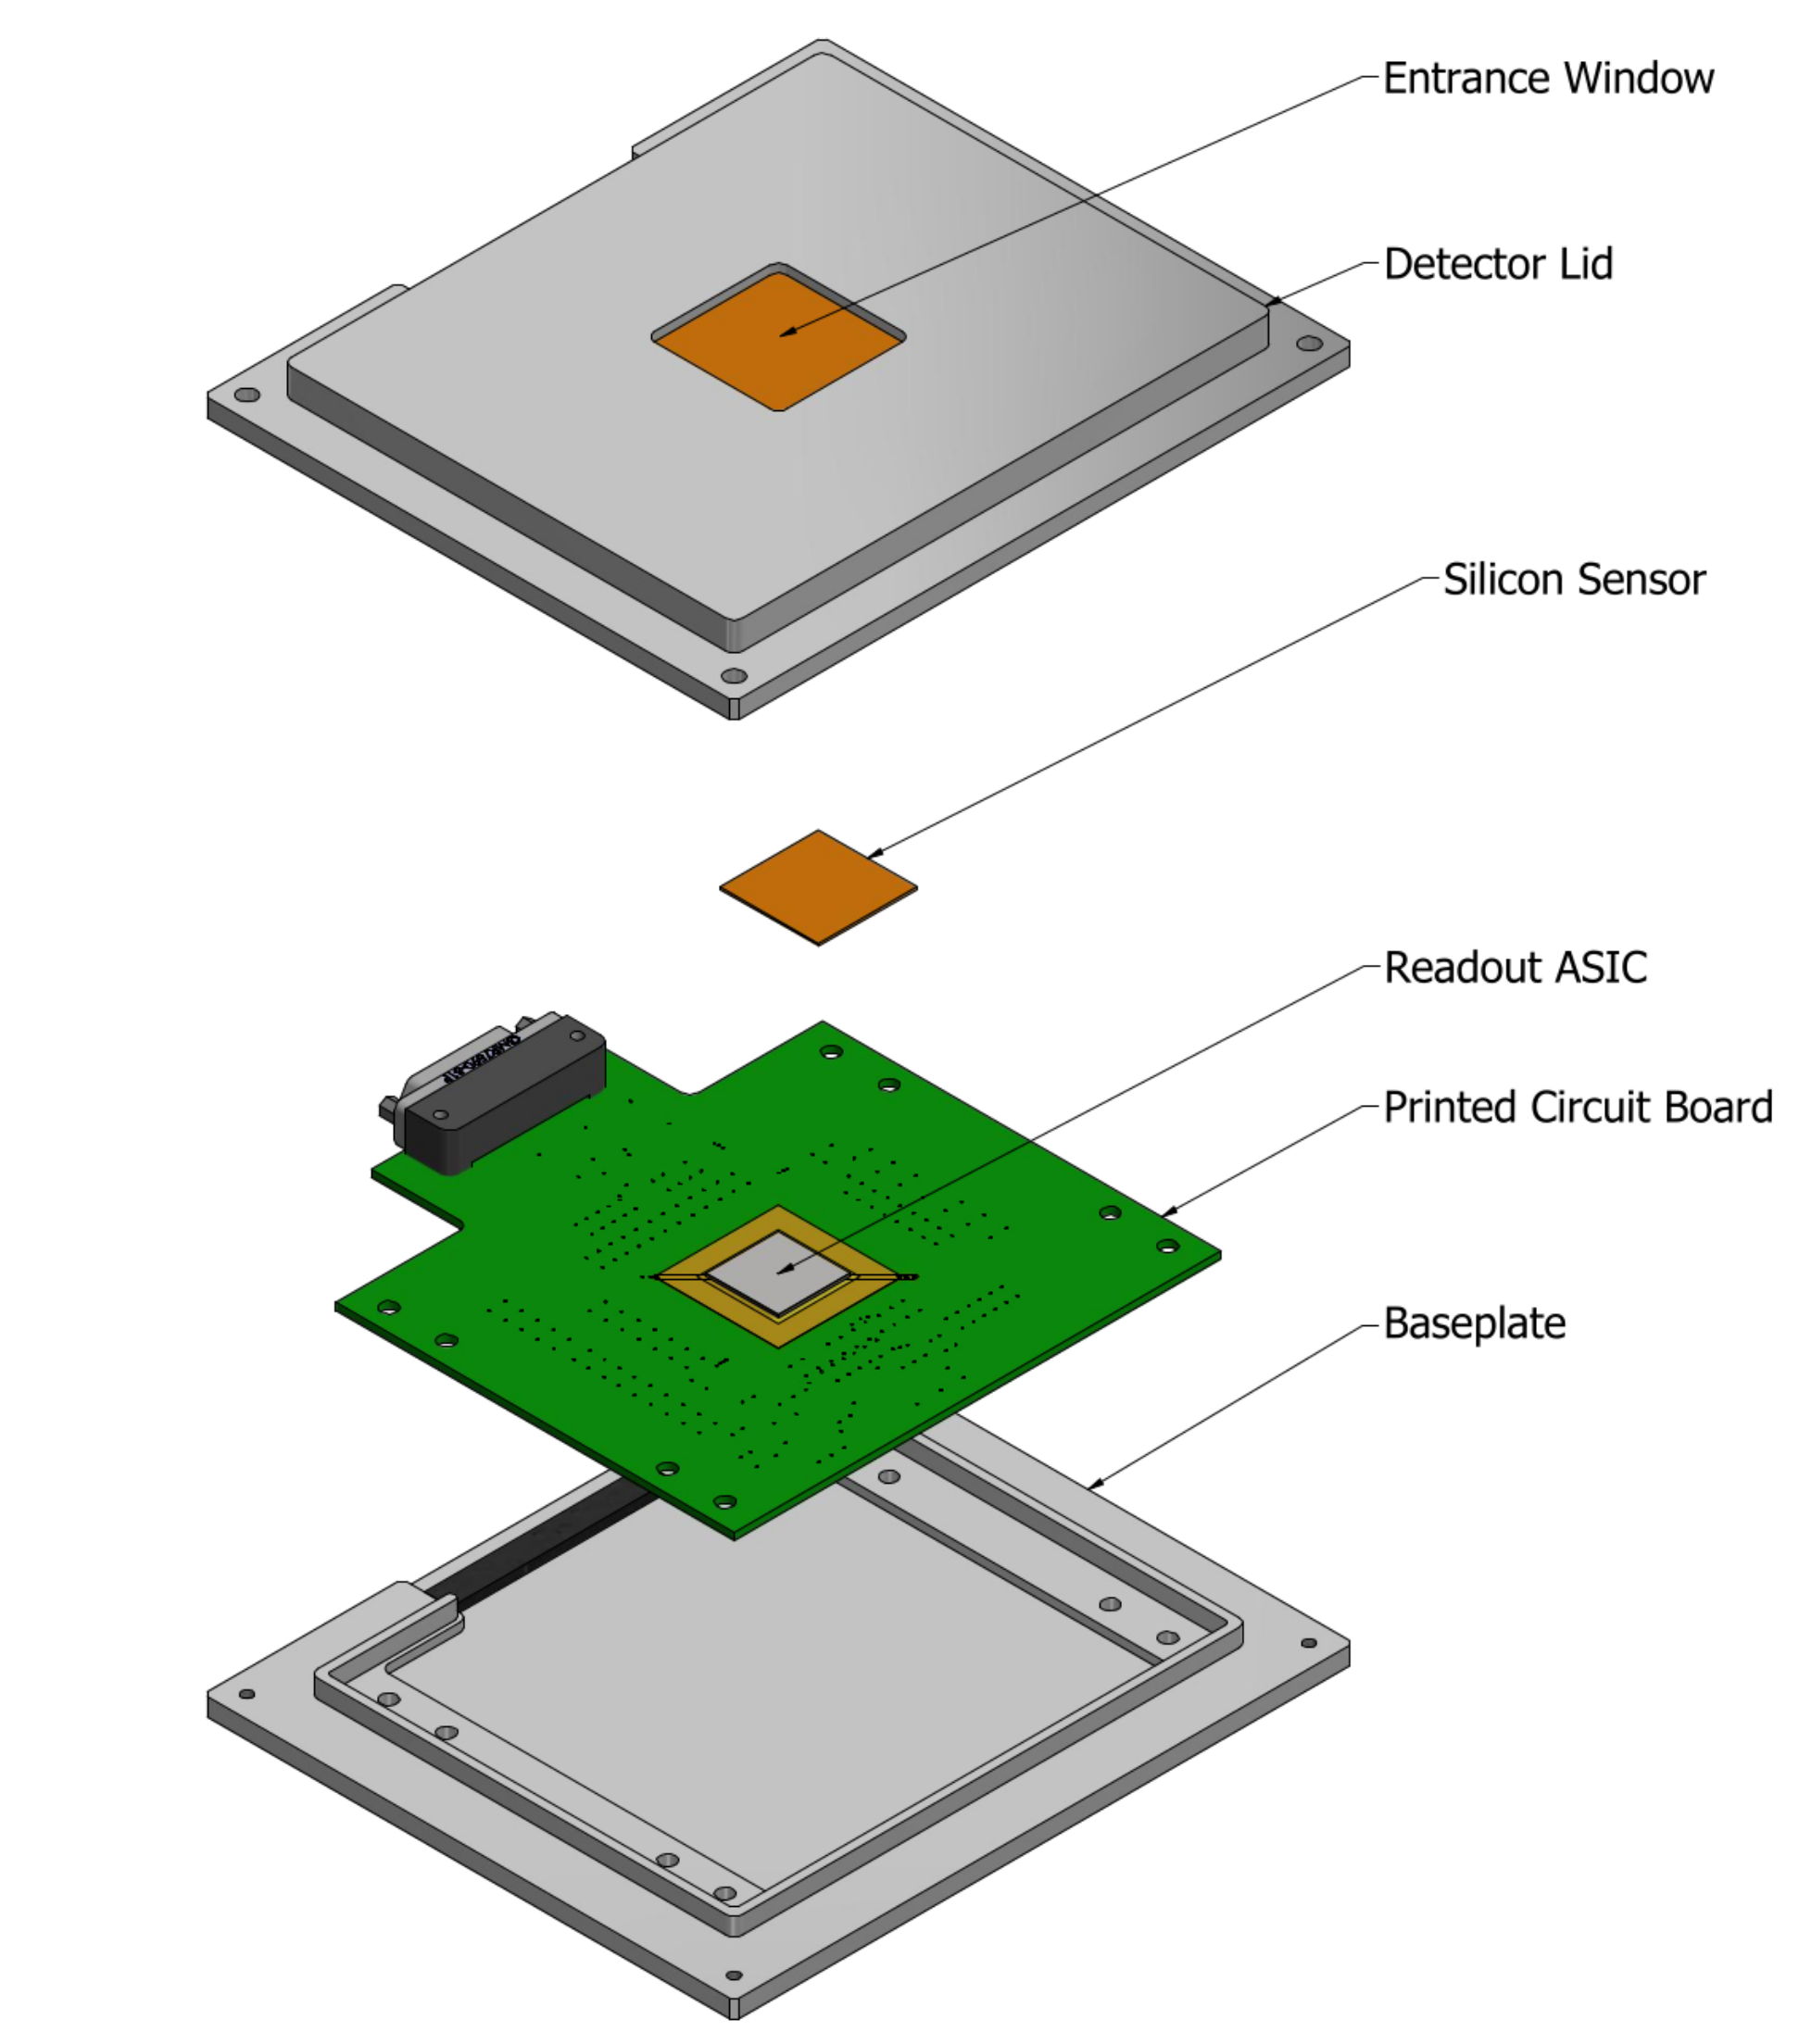
\includegraphics[width=0.7\linewidth]{figures/chapter4/design/detector}
    \caption{Exploded view of the detector with its housing. The detector is placed inside a simple metal housing with a square entrance window of a material suited for X-ray detection, such as beryllium or plastic materials. The detector itself is composed of the semiconductor sensor bump-bonded on top of the readout ASIC, which is wire bonded to the electronic board.}
    \label{fig:detector}
\end{figure}


\subsection{Active sensor}
\label{subsec:sensor}

The active sensor is the component of the detector where the physical signal is generated by interaction mechanisms between radiation and the sensor material, which is ionized by charged particles or by the photoelectron generated by the absorption of electromagnetic radiation \cite{rossi2006}. In solid state detectors the active sensor is made of a semiconductor material. 

There are various choices for the sensor material, depending on the required properties of the detector and the type or radiation that has to be detected. ASIX, which is designed to work with soft and hard X-rays, currently employs silicon and cadmium-telluride (CdTe) in the two prototypes currently available. CdTe is best suited for the harder region of the electromagnetic spectrum, as cadmium and tellurium are high-$Z$ materials, thus they have a cross section higher than silicon and a higher photoabsorption efficiency, as shown in Figs. \ref{fig:photo_cross_section} and \ref{fig:photoabs}.

The two active sensor prototypes consist of an hexagonally pixelated n-on-p 300 $\mu$m thick silicon sensor with a pixel pitch of 50 $\mu$m and an hexagonally pixelated Schottky-type 750 $\mu$m thick CdTe sensor with a pixel pitch of 100 $\mu$m \cite{minuti2025}, shown in Fig. \ref{fig:cdte_proto}. Given that the currently available ASIC readout chip has hexagonal pixels with 50 $\mu$m pitch, the CdTe sensor requires to connect one out of every four readout pixels.

\begin{figure}
    \centering
    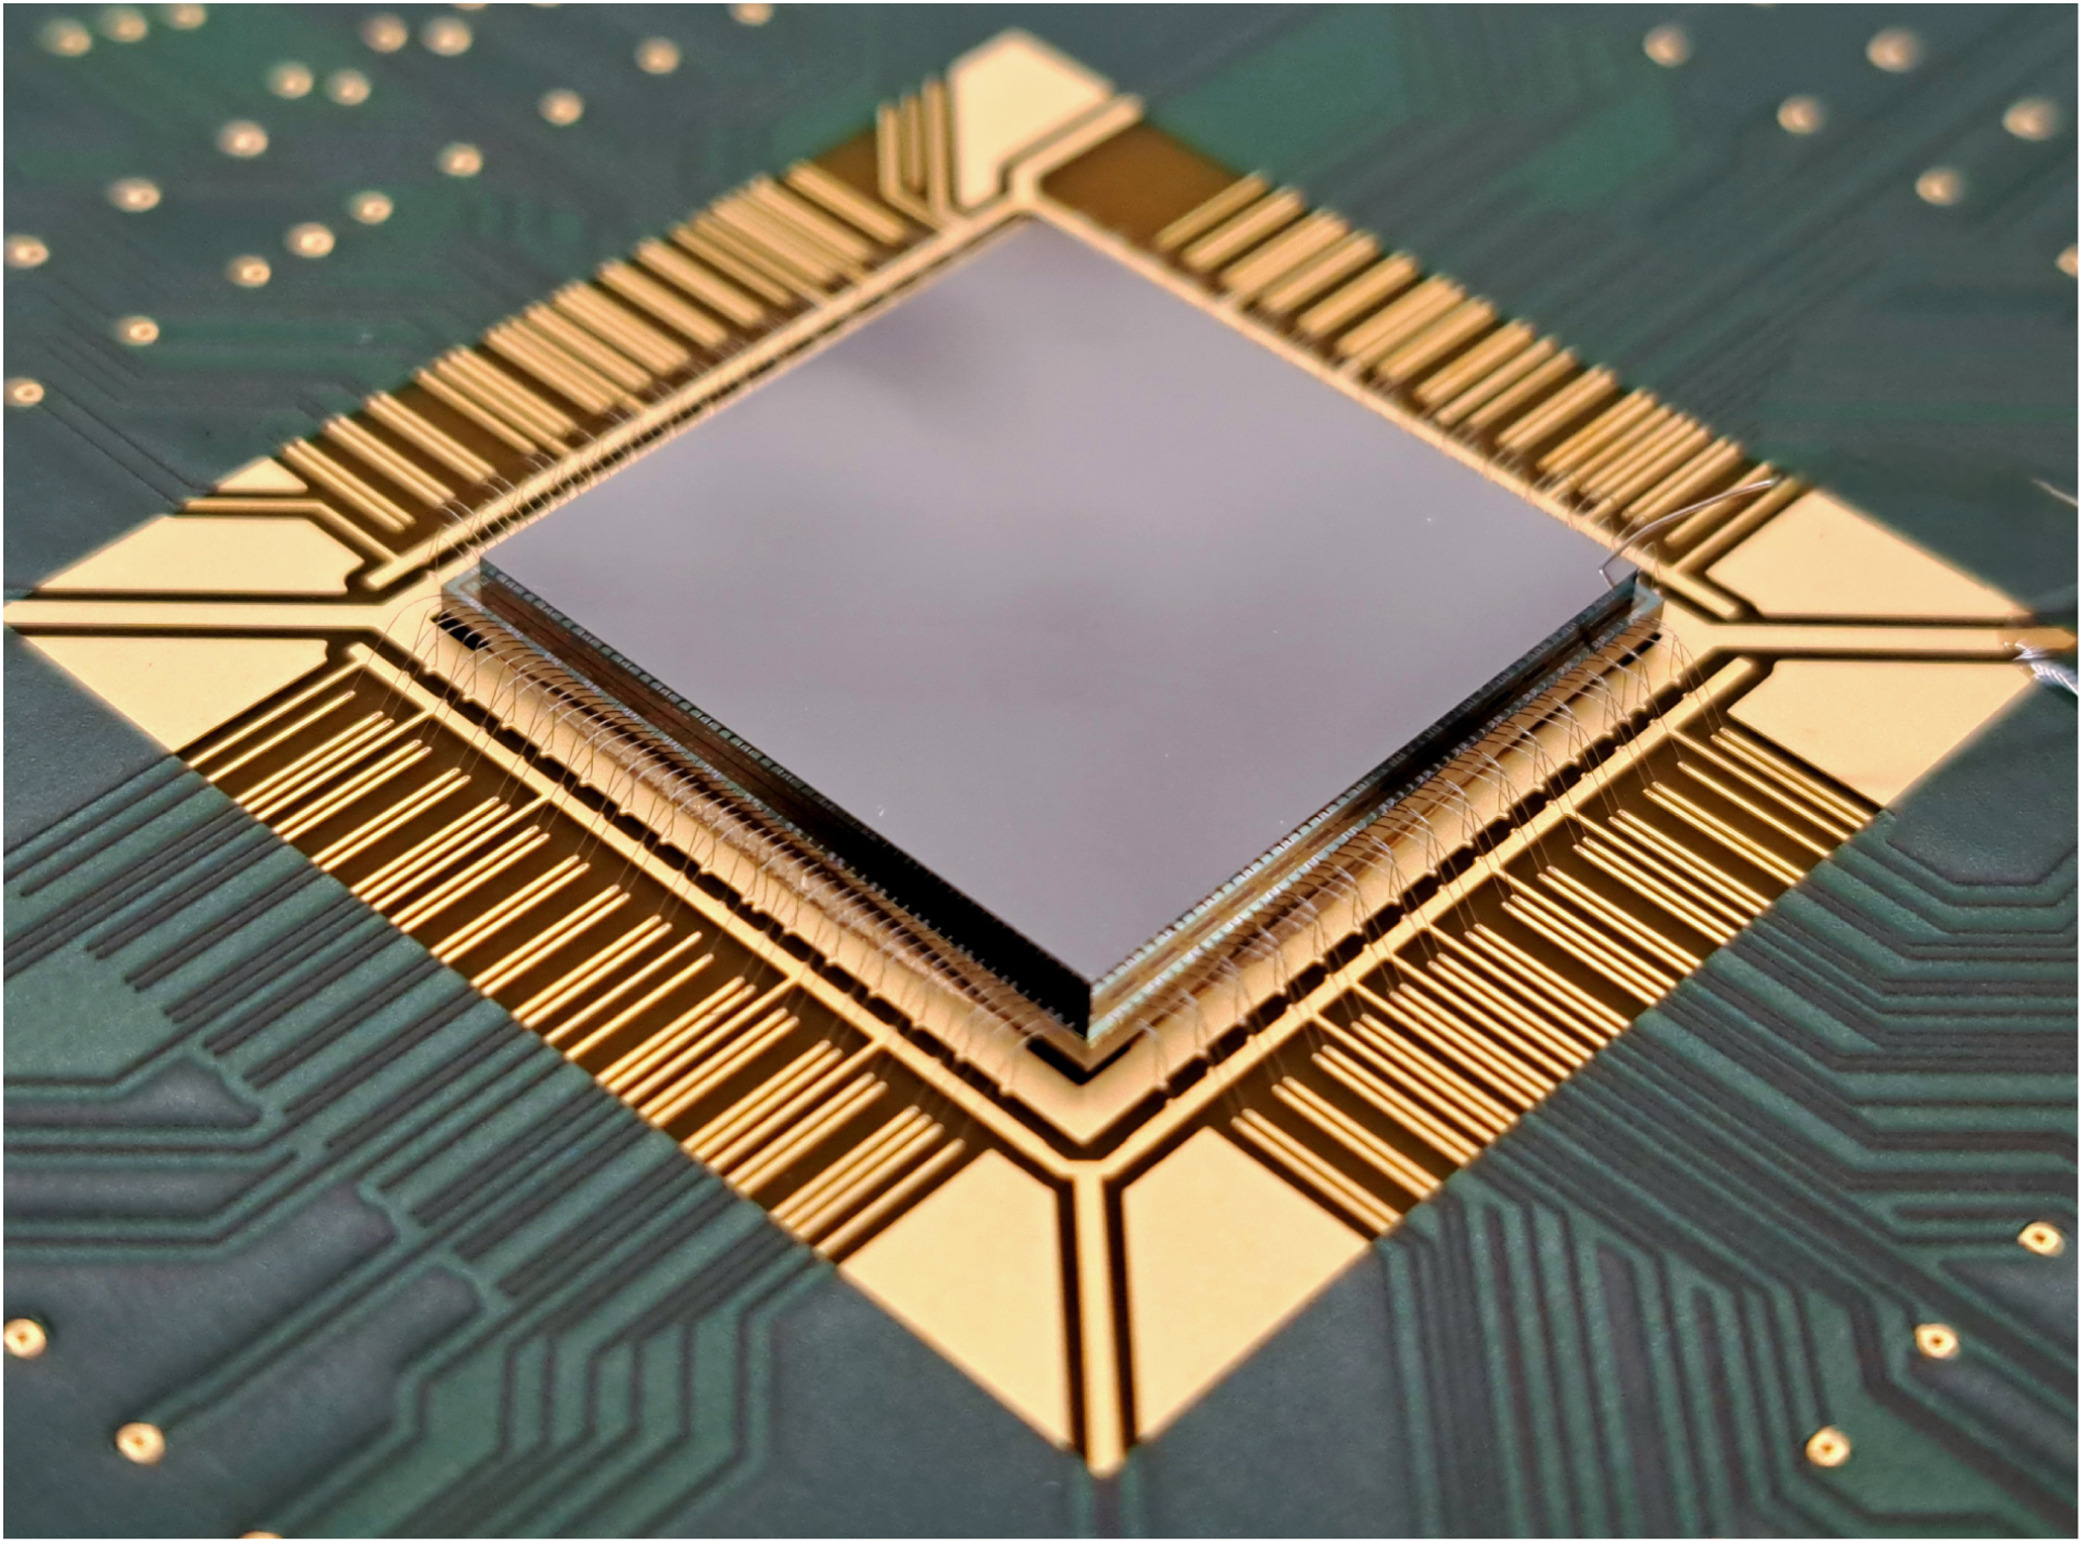
\includegraphics[width=0.7\linewidth]{figures/chapter4/design/asix}
    \caption{ASIX hybrid pixel detector with the CdTe sensor. The metallic layer visible on top is a platinum electrode positioned on the back side of the CdTe sensor to apply the reverse bias voltage. Image taken from \cite{minuti2025}.}
    \label{fig:cdte_proto}
\end{figure}

When a photon is absorbed in the active sensor, the distance traveled by the photoelectron depends on its kinetic energy and the sensor material, but it is typically much smaller than the sensor thickness (e.g., in silicon for $E_{\gamma} < 10~\text{keV}$, the photoelectron range is less than $1~\mu\text{m}$ \cite{nist_estar}). Consequently, the region where electron-hole pairs are generated via ionization can be approximated as point-like and coincident with the photon absorption point.

Once electron-hole pairs are generated they start to diffuse in the plane perpendicular to the electric field, as described in Chap. \ref{sec:semiconductors}. Knowing the sensor material properties, the electric field and the working conditions of the detector (e.g. the sensor temperature), the transverse diffusion sigma can be calculated using Eq. \ref{eq:diff_sigma_dist}.

The absorption depth depends on the energy of the photon and is distributed according to Eq. \ref{eq:pdf_truncated}, and by fixing the sensor thickness it allows to calculate the mean transverse diffusion sigma $\langle \sigma \rangle$ from Eqs. \ref{eq:z_average} and \ref{eq:diff_sigma_dist}. The dependence of $\langle \sigma \rangle$ on the photon energy for different Si sensor thicknesses is shown in Fig. \ref{fig:mean_sigma}.

\begin{figure}
    \centering
    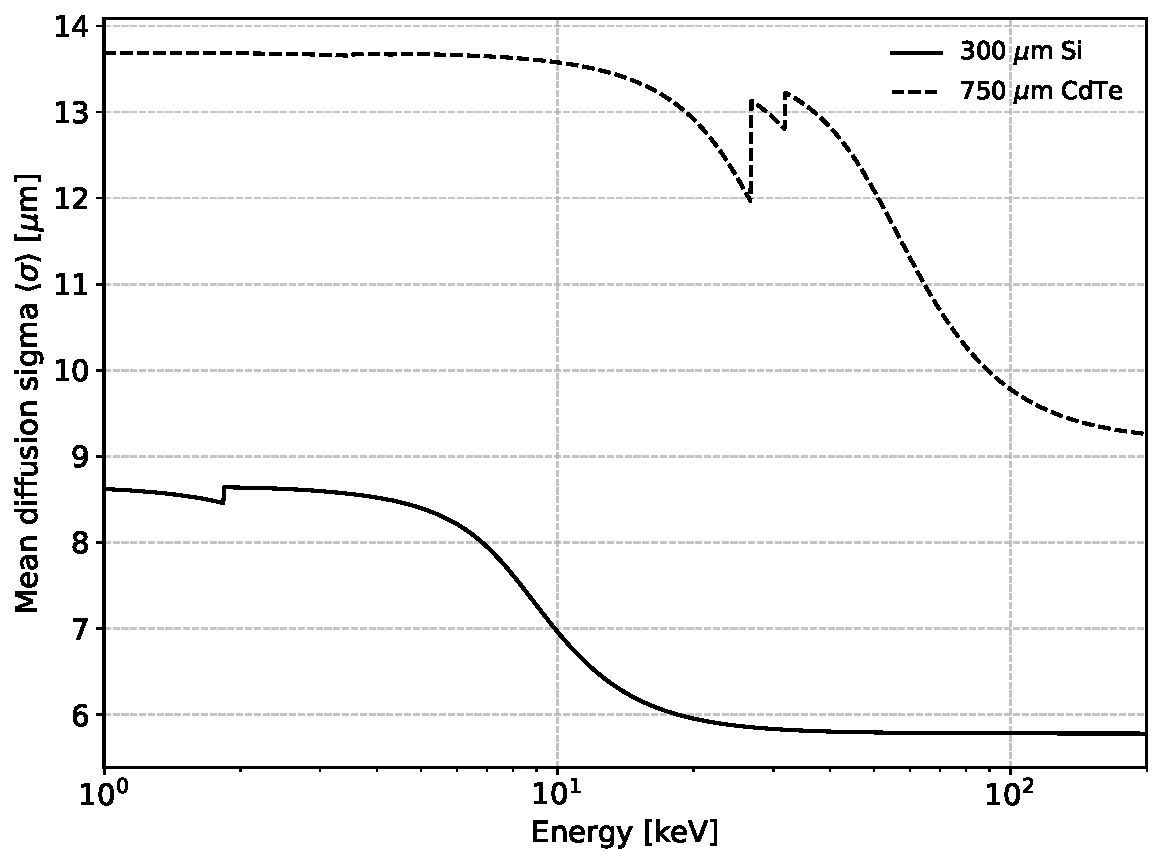
\includegraphics[width=0.7\linewidth]{figures/chapter4/design/mean_diffusion}
    \caption{Mean diffusion sigma as a function of the photon energy for different thickness of Si sensors, assuming $\mathcal{D} = 50 \,\mu$m cm$^{-0.5}$. }
    \label{fig:mean_sigma}
\end{figure}

Once the sensor working conditions like the temperature and the electric field are determined, meaning that $\mathcal{D}$ is fixed, Eq. \ref{eq:z_average} allows to find the best values of the sensor thickness and pixel pitch depending on the main intent of the detector.

If the goal is an imaging detector, the best choice would be to produce a large charge diffusion cloud in order to hit a lot of pixels and then reconstruct the position even with simple algorithms. Conversely, for spectroscopy applications, the smaller the number of pixels involved in the event, the better the energy resolution, as the total readout noise on the final measurement scales as $\sqrt{N}$, where $N$ is the number of pixels involved.

ASIX's goal is to find a compromise between an imaging and a spectroscopy detector, and thanks to a low noise readout and the pixel size and geometry, a good performance for both tasks is achievable. For this reason the sensor thickness and pixel pitch are chosen in order to have a ratio between the charge diffusion sigma and the pixel pitch $\langle \sigma \rangle / p$ in the range between 10--20\%.

The relevant metric to gauge how this ratio affects the detector readout design and the event analysis is the cluster size, which is defined as the number of pixels that have a signal above a certain threshold.

Simulations of charge diffusion show that in this range of $\langle \sigma \rangle / p$ the cluster size is always smaller than eight. This means that, given the hexagonal geometry of the pixels, all the charge is contained inside a circular set of seven pixels, with the pixel with the most charge at the center of the set and the other six pixels arranged in a circular corona around it. As will be discussed in Chap. \ref{subsec:readout}, this feature defines the readout logic of the chip under development.

Another important property which depends on diffusion and detector geometry is how the charge is distributed across the pixels. This is essential to determine the imaging and spectroscopy performance of the detector. As shown in Fig. \ref{fig:charge_distr}, by analyzing simulated events uniformly distributed across the pixels, the pixel charge distribution is highly asymmetrical and on average more than 90-95\% of the charge is always collected by two pixels and the third pixel collects almost all of the remaining charge, while the other four pixels always have less than 1\% of the total charge.

In real working conditions, even with low-noise readout electronics, is highly probable that the charge collected by each one of these four pixels is comparable to the electronic noise or even smaller. 

\begin{figure}
    \centering
    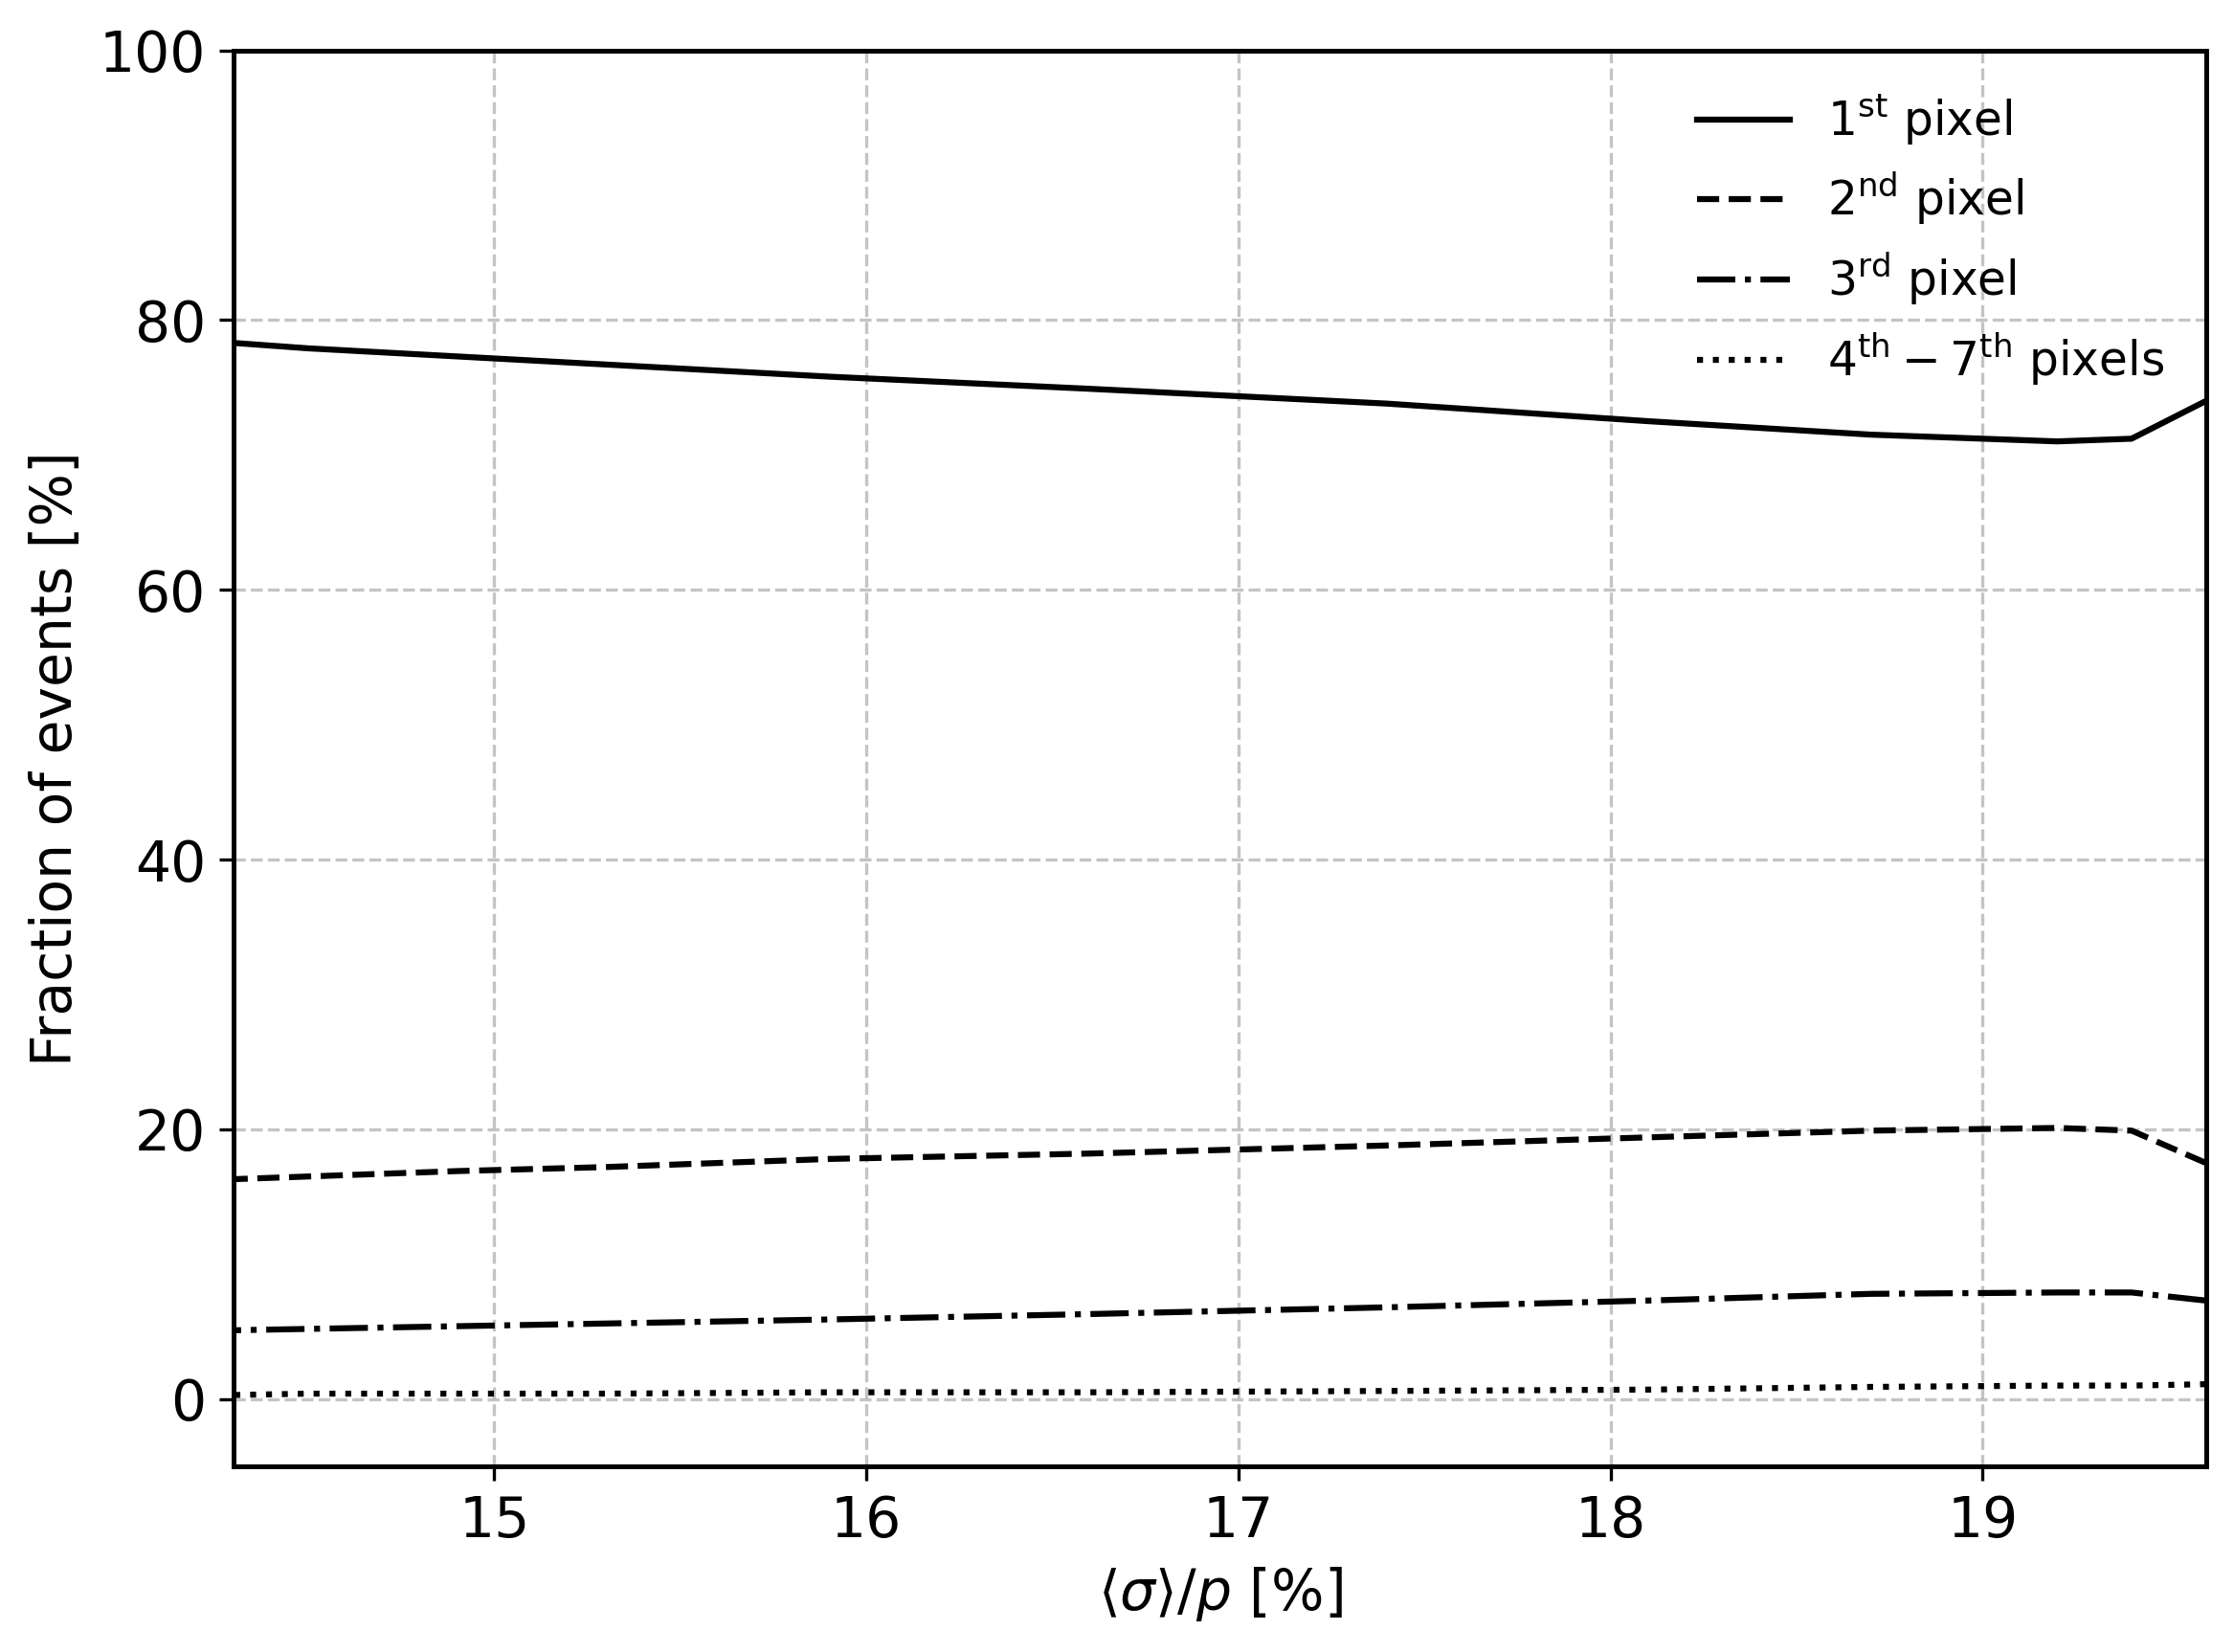
\includegraphics[width=0.7\linewidth]{figures/chapter4/design/charge_distr}
    \caption{Average charge fraction collected by the first, second, third and the remaining pixels as a function of $\langle \sigma \rangle / p$. The data set used consists of a simulation with uniformly distributed events across the pixels without electronic noise and no clustering threshold has been used.}
    \label{fig:charge_distr}
\end{figure}

%\begin{table}[htbp]
%\centering
%\begin{tabular}{c cccc}
%\multirow{2}{*}{$\langle \sigma \rangle / p$ [\%]} & \multicolumn{4}{c}{Pixel charge [\%]} \\
%\cmidrule(lr){2-5}
% & 1 & 2 & 3 & 4--7 \\
%\midrule
%19.6 & 74.0 & 17.5 & 7.3 & 1.1 \\
%19.4 & 71.2 & 19.9 & 7.9 & 1.0 \\
%19.2 & 71.0 & 20.1 & 7.9 & 1.0 \\
%18.7 & 71.5 & 19.9 & 7.8 & 0.9 \\
%18.1 & 72.5 & 19.4 & 7.3 & 0.7 \\
%17.4 & 73.8 & 18.8 & 6.8 & 0.6 \\
%16.6 & 74.9 & 18.2 & 6.3 & 0.5 \\
%15.9 & 75.8 & 17.8 & 5.9 & 0.5 \\
%15.3 & 76.7 & 17.2 & 5.6 & 0.4 \\
%14.9 & 77.3 & 16.9 & 5.4 & 0.4 \\
%14.5 & 77.9 & 16.5 & 5.2 & 0.4 \\
%14.3 & 78.3 & 16.3 & 5.1 & 0.3 \\
%\bottomrule
%\end{tabular}
%\caption{Average charge fraction collected by cluster pixels for different values of the ratio between the mean transverse diffusion sigma and the pixel pitch. The simulated data set is the same as Tab. \ref{tab:cluster_size}. It can be observed that the majority of the charge is collected by the first three pixels. \fix{Sostituire con grafico in cui su asse x c'è s/p, su y mettiamo occorrenza, plottiamo 1 pixel, 2 pixel, 3 pixel, sum(4-7) pixel, magari anche sum(1-2)}}
%\label{tab:charge_distr}
%\end{table}

\subsection{Readout strategy}
\label{subsec:readout}

The major difference between a GPD and the detectors developed under the ASIX project lies in the track topology. In a GPD, a photoelectron track can be up to a millimeter long (tens of pixels) due to the low density of the gaseous active medium, and its morphology varies significantly with photon energy. In a solid-state detector, instead, the charge is confined within a few tens of micrometers (a few pixels, typically no more than three, and strictly fewer than eight), as shown in Fig. \ref{fig:charge_distr}.

Furthermore, the charge distribution is axially symmetric around the impact point. As previously mentioned, this topology results in an event that is fully contained within a region composed of a central pixel (which collects most of the charge) and its six immediate neighbors.

Given this fixed maximum dimension and geometry, the readout can be performed differently from that of a GPD. The core idea is that when a pixel exceeds the trigger threshold, it is read out together with all six surrounding neighbors, regardless of the charge they have collected; therefore, the readout process always involves a fixed geometry seven-pixel cluster.

This represents a remarkable difference with respect to GPDs, requiring a completely new chip designed to fully exploit the advantages offered by this compact event topology. An example of the readout strategy is shown in Fig. \ref{fig:adc_routing}.

\begin{figure}[htbp]
    \centering
    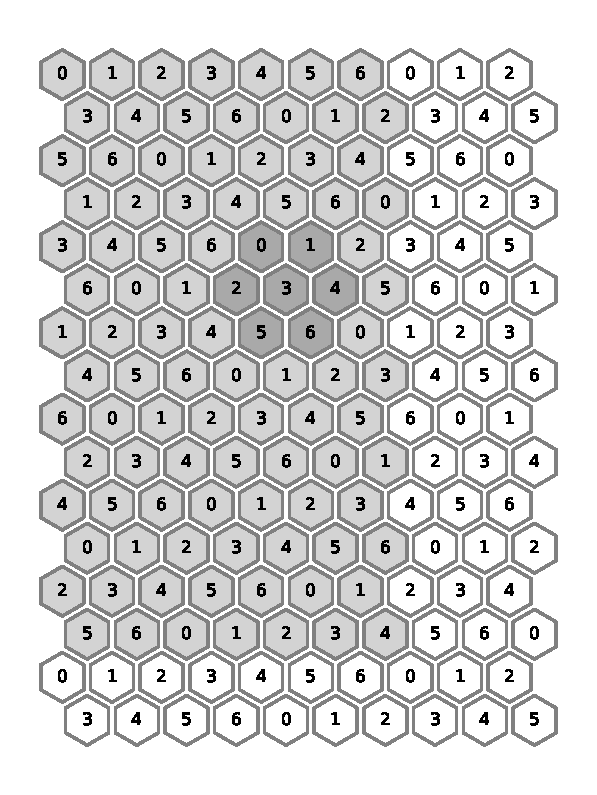
\includegraphics[width=0.4\linewidth]{figures/chapter4/design/adc_routing}
    \caption{Example of pixel routing using seven independent ADC channels. Each pixel is labeled with its corresponding ADC channel. The light gray area highlights the minimal unit cell needed to avoid adjacent pixels sharing the same channel. The seven darker pixels illustrate a cluster read out after the pixel connected to channel 3 triggers the event.}
    \label{fig:adc_routing}
\end{figure}


\subsection{ASIC}
\label{subsec:asic}

The goal of developing a detector suitable for different applications under diverse operating conditions requires a readout chip capable of handling event rates significantly higher than those typical of astrophysical sources. As a reference, the brightest extrasolar source in the 2--8~keV energy range yields a flux of about 30~ph~cm$^{-2}$~s$^{-1}$, whereas an XRD laboratory setup with a Cu source can easily exceed a flux of $2 \times 10^8$~ph~cm$^{-2}$~s$^{-1}$ \cite{bolze2019}.

The key to speeding up the readout with respect to GPDs is exploiting the fixed event geometry. While reducing the number of pixels to read is essential to lower the dead time, the main architectural breakthrough is the ability to read all seven pixels in parallel. 

This parallel readout can be implemented using an external ADC with seven independent channels. Each pixel in a cluster is routed to a different channel, and the hexagonal honeycomb arrangement of the pixels is ideal for this purpose, as it allows the entire chip matrix to be mapped using seven channels without any adjacent repetition of the same channel. This configuration enables a 7-pixel cluster to be read out in parallel at any location on the chip, as illustrated in Fig. \ref{fig:adc_routing}.

A further increase in rate capability can be achieved by segmenting the chip into independent readout regions, each equipped with its own 7-channel ADC. Although this approach can truncate events occurring at the boundaries between regions, leading to their rejection, selecting an optimal region size and shape ensures that the fraction of rejected events remains negligible.

The current design goal is to achieve a maximum rate capability of at least 100~kHz per region at a readout clock frequency of 20~MHz, which translates into a global detector rate of about 1~MHz, depending on the final number of independent regions.

The minimal event structure for readout requires to save the coordinates of the highest pixel (9 + 9 bit for a $304 \times 352$ pixels chip), the content of the pixels ($12 \times 7$ bit, assuming to use a 12 bit ADC) and the timestamp (16 bit), with a total event size of 118 bit. With a global rate of 1 MHz it would require a data bus with the capability of transferring around 100 MBit/s, which is feasible.

This performance estimate assumes that pedestal subtraction is performed offline, unlike in previous XPOL chips. Indeed, since all seven pixels are sampled simultaneously by their dedicated ADC channels, systematic effects induced by time-dependent digital transients during serial readout are naturally avoided. This eliminates the need for a second pedestal readout pass, saving time at the cost of requiring an accurate offline pedestal calibration.

Another critical property, essential for high-resolution spectroscopy, is the Equivalent Noise Charge (ENC) introduced by the front-end electronics. The design target is to maintain the noise below 20~$e^-$ ENC per pixel. When coupled with a silicon sensor, this noise level yields an energy resolution of approximately 350~eV FWHM at 8~keV, which is sufficient to resolve the Cu-K$_{\alpha}$ (8.04 keV) and Cu-K$_{\beta}$ (8.90 keV) fluorescence lines commonly used in XRD setups.

All these requirements are achievable with a dedicated analog front-end ASIC. The proposed design features $50~\mu\text{m}$ pitch hexagonal pixels in a honeycomb array over a rectangular matrix, similar to the other XPOL family chips. However, unlike in GPDs, where the readout pixels are physically separated from the GEM, in the ASIX architecture the ASIC pixels are directly connected to the pixelated sensor via micro-bump soldering, aligning each ASIC pixel to the corresponding electrode on the sensor.

Finally, to preserve the chip versatility for applications such as X-ray polarimetry, it will be designed to support an alternative triggering and readout logic similar to XPOL-III, based on a sequential readout within a rectangular ROI, as described in Chap. \ref{sec:xpol3}. While this mode operates at lower speeds and reduced maximum rates, it allows the acquisition and reconstruction of extended photoelectron tracks when required.

At the moment, the dedicated ASIC is still in the design phase and prototypes are not yet available.

\section{Simulations and analysis framework}

To estimate the properties of different detector designs prior to the realization and then to characterize a prototype, a framework to generate Monte Carlo simulations of the detector and analyze collected data has been developed and is available at \cite{hexsample, tomaiuolo2024}. The framework provides a suite of command-line tools that can be executed directly from the terminal or integrated into automated scripts. Data are stored using the Hierarchical Data Format (HDF5), which allows for efficient array storage and metadata tagging through file attributes. The core pipeline modules, illustrated in Fig.~\ref{fig:block_diagram}, are responsible for running Monte Carlo simulations, converting raw binary data collected with prototypes into HDF5 files, performing detector calibration, and executing event reconstruction.

This section illustrates the Monte Carlo simulation software and the calibration and analysis pipeline.

\begin{figure}[h]
    \centering
    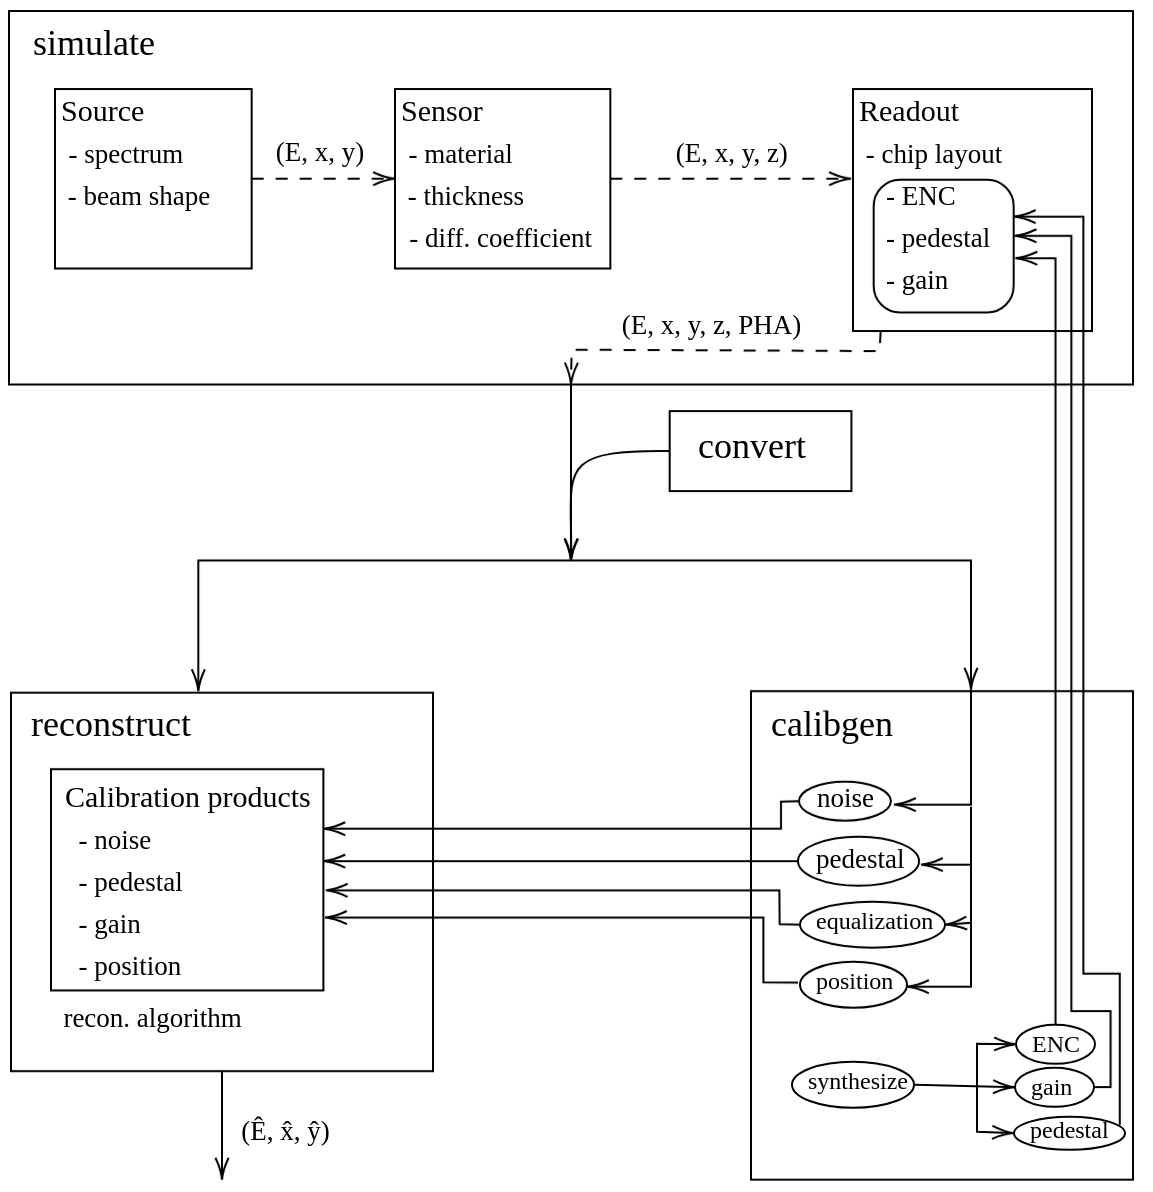
\includegraphics[width=0.7\linewidth]{figures/chapter4/calibration/block_diagram}
    \caption{Block diagram representing the main steps of the simulation and analysis software available at \cite{hexsample}. A dataset can be generated with the Monte Carlo simulation framework or obtained by converting a binary laboratory acquisition. The dataset is used to generate the calibration products, which are subsequently employed to reconstruct the events.}
    \label{fig:block_diagram}
\end{figure}

\subsection{Monte Carlo simulations}
Monte Carlo simulations of the detector are essential to understand its capabilities depending on the design. As mentioned in the previous section, designing a detector which has both imaging and spectroscopical high-resolution capabilities requires to carefully tune the active sensor thickness, pixel pitch, working voltages and further properties to achieve the correct trade-off between energy and spatial resolution. 

With the first prototypes it is also possible to validate the simulations with laboratory data, and if necessary finely tuning the Monte Carlo to match the data, in order to have a software that can reliably simulate the real detector. The simulation consists of different steps, each representing a different stage of the detector.

First, it is necessary to define the detector design, specifying the active sensor and the readout chip properties. The active sensor is described by three parameters, which are the material, the thickness and the transverse diffusion coefficient of the electrons, defined in Eq. \ref{eq:diff_sigma_dist} and that depends on the working conditions.

The chip layout is described by the pixel pitch, the number of columns and rows and the readout logic, which allows to choose between the seven-pixels parallel readout and the XPOL-III sequential rectangular readout with the additional option to choose the padding dimensions. The readout chip is also characterized by three other quantities, the ENC, the pedestal and the gain, which are provided in form of matrices with the same dimension of the chip to take into account spatial variations across the chip. The last thing to setup is the X-ray source, which is described by its energy spectrum and the beam shape, position and spatial distribution.

In the simulation, a photon with a given energy and incident position is generated according to the spectrum and beam distribution and then its absorption depth is sampled from Eq. \ref{eq:pdf_truncated}.

At the moment, only on-axis photons generation is implemented. Furthermore, the approximation that electron-hole pairs are produced in a point-like region located in the absorption point is adopted. As mentioned above, this approximation is valid in the case of a silicon sensor and photon energies below 10 keV.

The diffusion is modeled as discussed in Chap. \ref{subsec:sensor}, assuming a two-dimensional Gaussian distribution centered on the impact point and with a standard deviation which depends on the absorption depth. Afterwards, the event readout is performed according to the chosen readout logic.

The simulation does not take into account some physical effects, such as the distance travelled by the photoelectron or the possibility of having a fluorescence photon that can travel through the sensor before being absorbed, with the consequence that a point-like conversion region is no more a good approximation.

As mentioned above, the first effect becomes relevant at high photon energies, while the second effect depends on the photon energy and the sensor material, as fluorescence yield depends on the involved shell and on the atomic number $Z$. For silicon the fluorescence yield is smaller than 5\% for K-shell and almost 0\% for L-shell, while for cadmium and tellurium is between 83-88\% for K-shell and about 5-7\% for L-shell, as shown in Fig. \ref{fig:fluorescence_yield}.

If fluorescence radiation is emitted, given the isotropic emission angle distribution, it travels through the sensor until it is absorbed and produces a new photo-electron. Depending on the photon energy, the new photoelectron can be generated even a pixel pitch far from the first electron. For CdTe sensor this drastically decreases the simulation accuracy, but only for energies above the K-edge, which is about 27 keV.

At the moment the goal of the simulation software is to validate and verify the feasibility of the silicon sensor design in the 6--10 keV energy range, thus all of these effects are negligible. In the future more detailed simulations will be performed by implementing this stage with Geant4 \cite{geant4}.

Another effect that is not taken into account is pixel crosstalk, which represents an additional source of charge sharing between pixels. A simple way to partially solve this is to include this effect into the charge diffusion process, increasing the diffusion parameter calculated from Eq. \ref{eq:diff_sigma_dist}. The correct value of this parameter can be chosen comparing the cluster size distribution between laboratory data and simulation until they match.

\subsection{Analysis}
\label{sec:analysis}
After detector calibration, which requires more details and will be explained in the next section, data files generated with Monte Carlo simulations or by converting laboratory binary data files can be analyzed to extract the relevant information about the events.

Each event contains information about the timestamp, the signal amplitude recorded by each pixel (expressed as Pulse Height Amplitude, or PHA), and the coordinates needed to localize the event, which depend on the readout mode. If using the seven-pixel parallel readout mode the coordinate of the central pixel is given, while in the XPOL-III readout mode the coordinates of two opposite vertices of the rectangular ROI and the padding information are stored.

Detector calibration is necessary because raw PHA values need to be corrected for two contributions, which are pedestal and normalized gain variations over the chip. Further details will be given in the following.

The corrected PHA values are used to analyze the event and reconstruct photon properties, such as energy and impact position. The reconstruction software contains different algorithms to infer the position and energy, and according to the one adopted an additional processing of the data can be required.

For some algorithms all the PHA values of the seven-pixel cluster are necessary, while for others a data reduction can be made. Particularly, as shown in Fig. \ref{fig:charge_distr}, more than 99\% of all the charge is collected by the three pixels with most signal. This information can be used to create a smaller cluster containing only pixels that have a high probability of having collected physical signal and not only electronic noise.

The first step to create the cluster is choosing a zero-suppression threshold, which is defined for each pixel in terms of its noise standard deviation, measured during the calibration phase to build a dedicated noise map of the chip. The threshold is used to suppress all the pixels that are dominated by electronic noise.

The second step applies a geometrical constraint, requiring all pixels above threshold to be adjacent. The central pixel is always kept as it triggered the event. The remaining pixels in the cluster are selected by evaluating the non-central pixels above threshold in descending order of signal amplitude, starting from the one with the highest PHA. A pixel is kept only if it is adjacent to a previously accepted pixel, otherwise it is suppressed. This process continues until a maximum of two neighboring pixels (plus the central one) is reached. Consequently, the final cluster size is strictly constrained to be between one and three.

\section{Detector calibration}
\label{sec:calibration}

Raw PHA values recorded by the detector need to be corrected for electronic baseline offsets (pedestal) and pixel-to-pixel gain variations (equalization) to retrieve the true deposited charge. Furthermore, characterizing the pixel noise is essential to define zero-suppression thresholds and to correctly weight PHA values during clustering and event reconstruction.

Detector calibration is crucial to account for spatial non-uniformities across the active area, which arise from small imperfections in the readout electronics, sensor inhomogeneities, and non-uniformities in the bump-bonding connections with the ASIC. Correcting for these variations allows maximizing detector performance and improving both spatial and energy resolution.

The calibration process consists in measuring the pedestal level (in ADC counts), the noise standard deviation (in ADC counts), and the normalized gain for each pixel across the matrix. The resulting maps are employed during event reconstruction to subtract offsets, set noise-dependent thresholds, and equalize the pixel response. Under specific conditions, it is also possible to derive the absolute gain and the ENC noise by combining these calibration products with additional information on the incident radiation.

In the analysis framework a calibration product has been designed as an HDF5 file containing three different matrices with the same shape as the readout chip. Each element of a matrix is associated with the pixel in the corresponding position. The labels of the three matrices and their content are the following:
\begin{itemize}[label=-]
\item \textit{values}, contains the central value of the calibrated quantity for each pixel;
\item \textit{entries}, contains the number of events used for the calibration for each pixel;
\item \textit{errors}, contains the estimated uncertainty associated with the value of the calibrated quantity for each pixel.
\end{itemize}

The calibration products can either be generated by analyzing a data file or by synthesizing maps with the chosen size and values distribution. As said above, their main use is for event reconstruction, but they are also used to define the readout chip characteristics in the Monte Carlo simulation software.

When analyzing a data file, the calibration process follows a specific order. First, noise and pedestal levels are calibrated, and then the normalized gain is evaluated using these baseline products. If required, the absolute gain and ENC maps can subsequently be calculated using the ADC noise and normalized gain maps.

In this section the methods developed to calibrate noise, pedestal and gain are described, and finally the results obtained from the calibration of Monte Carlo simulations are presented to evaluate the performance of the calibration framework.

\subsection{Noise and pedestal}
\label{sec:noise_calibration}

Noise and pedestal variations are introduced by small non-uniformities in the manufacturing of the readout electronics and in the bonding of the active sensor onto the ASIC. Characterizing the noise of each pixel enables to apply pixel thresholds that take into account the possibility of having noisier pixels. 

The noise and pedestal level are estimated by sampling the PHA distribution of a pixel in the absence of source signal. Under this condition, the PHA distribution of each pixel is a Gaussian distribution with a mean corresponding to the pedestal and a standard deviation equal to the noise of the pixel. During the readout the Gaussian is truncated before 0 ADC and digitized. In the optimal configuration, to estimate both quantities, the pedestal is much larger than the noise and thus the Gaussian can be fully sampled. 

For the current prototypes, which are based on XPOL-III, it is possible to generate noise and pedestal maps from data acquisitions with a source that illuminates the chip.  As explained in Chap. \ref{sec:xpol3}, XPOL-III defines a ROT with triggered miniclusters and an additional padding can be added, with a large enough padding it is possible to have a lot pixels without source signal.

In the acquisitions used in the following the padding is large and the resulting ROI has a size of at least $10\times13$ pixels, as shown in Fig. \ref{fig:noise_pedestal_roi}. The true size depends on the number of miniclusters that triggered, thus it can be larger. Once the ROI is defined, pixels that belong to the ROT and all their neighbors are discarded in order to have the smallest probability of including pixels with source signal in the analysis. The number of pixels resulting from this selection is about 120, but it depends on the size of the ROT.

\begin{figure}
    \centering
    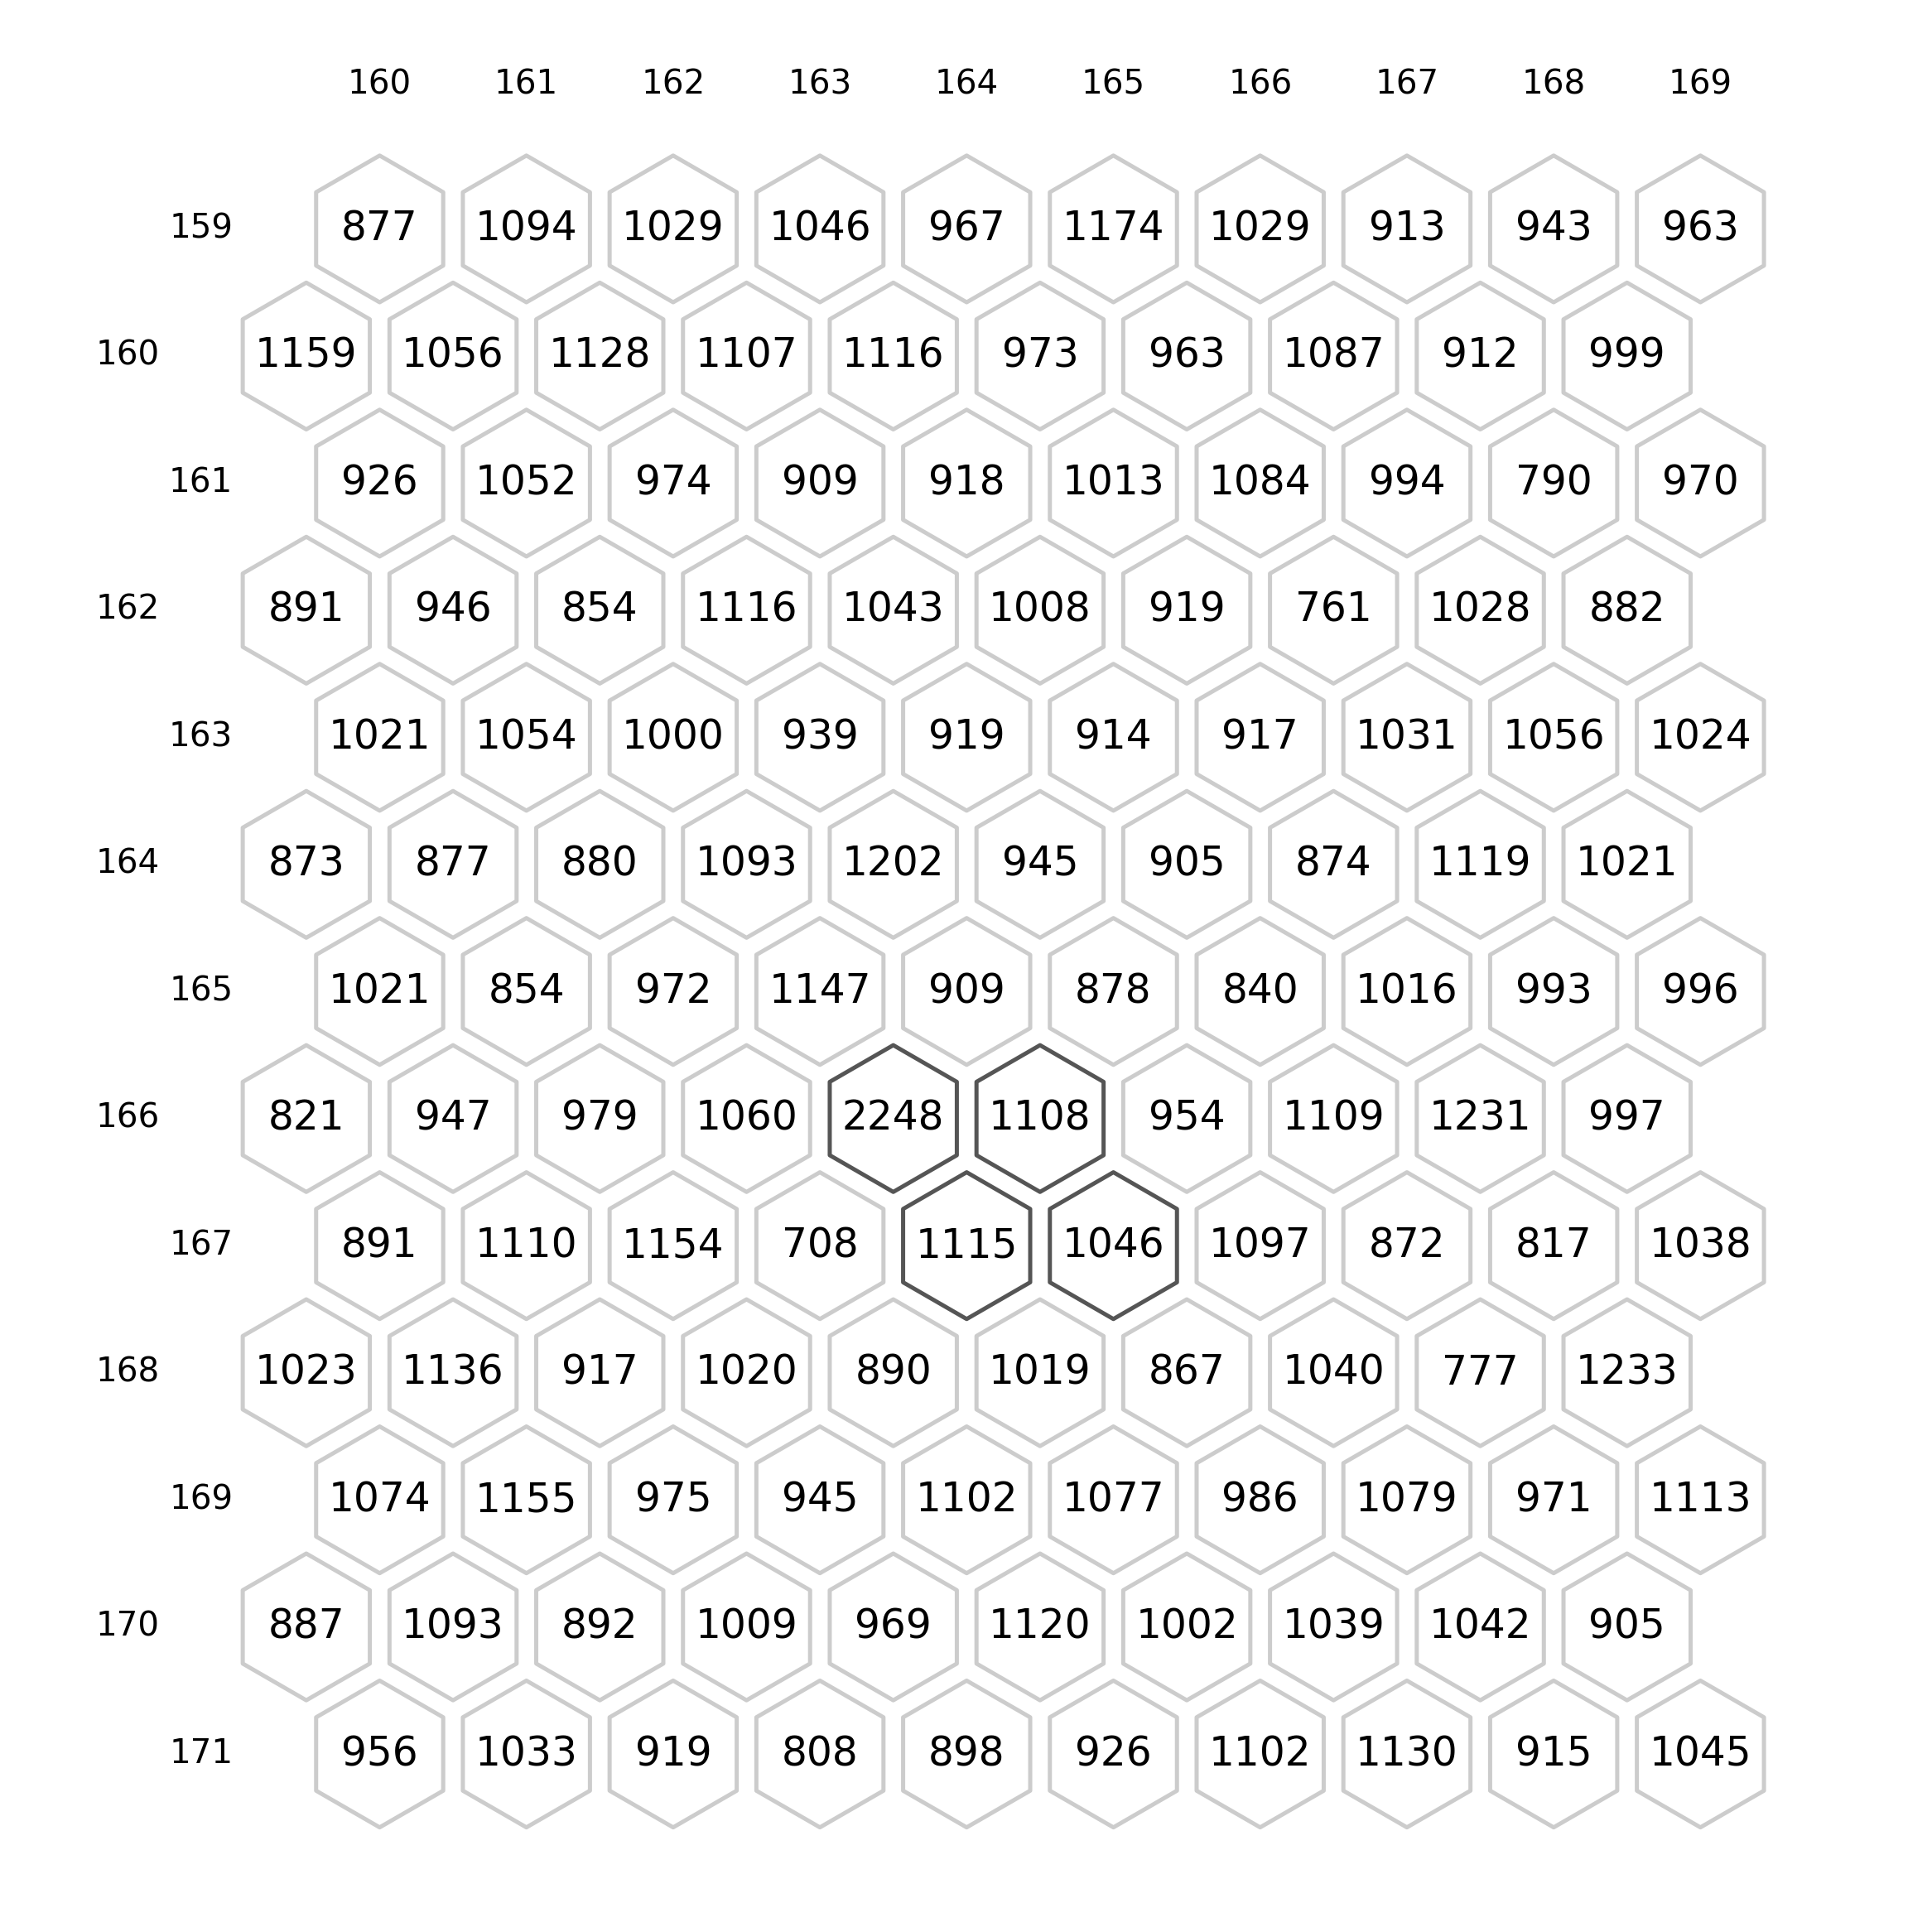
\includegraphics[width=0.5\linewidth]{figures/chapter4/calibration/roi}
    \caption{Example of the ROI of an event with the source on. Central pixels with marked borders belongs to the ROT and are excluded from the calibration analysis, together with all their immediate neighbors. This image is taken from a simulation with pixel noise and pedestals distributed according to Gaussian distributions with 20 ADC and 1000 ADC, respectively, and 10\% standard deviation.}
    \label{fig:noise_pedestal_roi}
\end{figure}

Depending on the readout properties, there are different methods that can be employed to calibrate noise and pedestals. However, in the current XPOL-III design pedestal subtraction is performed online, thus it is not possible to calibrate pedestal levels from data acquisitions. For this reason, it is assumed that they are exactly zero for all the pixels, thus only noise requires to be calibrated.

The first calibration method is used exactly in the current working condition where pedestals are zero. In this case the PHA sample distribution is a half-normal distribution defined only on the positive semi-axis, and the probability density function is

\begin{equation}
p(x; \sigma^2) = \frac{2}{\sqrt{2 \pi \sigma^2}} \exp \left( -\frac{x^2}{2\sigma^2} \right), \quad \text{for } x > 0
\label{eq:half_normal}
\end{equation}

Using the parity of the Gaussian it can be shown that the expectation value $\langle x^2 \rangle$ of the distribution defined in Eq. \ref{eq:half_normal} is equal to the variance of the untruncated Gaussian, which is exactly the square of the noise value to calibrate. The best-fit value of the pixel noise is thus given by

\begin{equation}
s = \sqrt{\frac{1}{N} \sum_i^{N} x_i^2}.
\end{equation}

The uncertainty related to this estimate is the uncertainty of the sample standard deviation, thus it is $s/\sqrt{2N}$.

In case the pedestal subtraction is performed offline, there are two possible cases in which it is possible to use different methods. The first is when the pedestal level is much larger than the noise, which is the optimal case and allows to sample the entire Gaussian distribution. On the other hand, the second case is when the pedestal level is comparable to the noise (not much smaller, otherwise the first method can be employed), thus the distribution is truncated on the left tail.

In the case where the pedestals are much larger (at least 4 or 5 times larger) than the noise it is possible to directly calculate the sample mean and standard deviation of the distribution. In practice, this method is performed using Welford algorithm \cite{welford1962} for online update of the mean and variance of each pixel distribution while looping on all the events of the acquisition. The mean and variance of the distribution after $n$ events are given by

\begin{equation}
\begin{split}
\bar{x}_n &= \bar{x}_{n-1} + \frac{x_n - \bar{x}_{n-1}}{n}, \\
M_{2,n} &= M_{2, n-1} + (x_n - \bar{x}_{n-1})(x_n - \bar{x}_n), \\
s_n^2 &= \frac{M_{2,n}}{n-1}.
\end{split}
\label{eq:welford}
\end{equation}

This method ensures very high numerical stability, is fast and the occupied space in memory only depends on the shape of the detector and not on the number of processed events. The error associated to the pedestal $\hat{p}$ is the uncertainty of the sample mean, and for the noise $\hat{n}$ is the one associated to the sample standard deviation, thus

\begin{equation}
\sigma_{\hat{p}} = \frac{\hat{n}}{\sqrt{N}}, \quad \quad \sigma_{\hat{n}} = \frac{\hat{n}}{\sqrt{2N}},
\label{eq:noise_uncertainty}
\end{equation}
where $N$ is the number of events collected for each pixel.

In the last case, when the pedestals are comparable to the noise, a least-squares minimization using a Gaussian curve as the fit model can be performed for each pixel. Furthermore, this method is not stable in the limit where the PHA distribution is a half-truncated digitized Gaussian because the fit rarely converges to acceptable values.

Fig. \ref{fig:methods} shows the possible cases of application of the three methods described above. At the moment the method employed on real data is the first, but all of them can be used when the new chip, whose design phase is not completed, will be ready.

\begin{figure}[t]
    \centering
    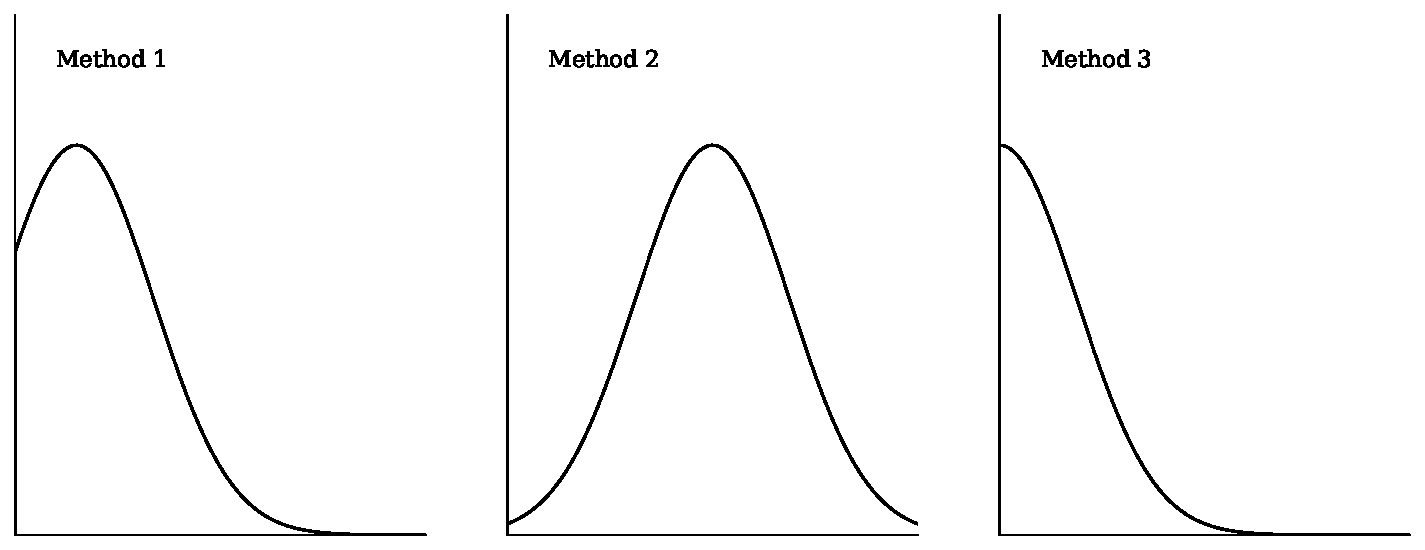
\includegraphics[width=1\linewidth]{figures/chapter4/calibration/noise_methods}
    \caption{Examples of applications of the different methods to estimate noise and pedestal levels of te detector. Method 1 can be applied when the pedestal is null and the distribution is a half-normal. Method 2 is ideal when the distribution is not truncated, thus the sample mean and standard deviation are correct. Method 3 is essential when the Gaussian is partly truncated, because the other methods do not converge to the correct values.}
    \label{fig:methods}
\end{figure}

For the first two methods the relative error on the noise calibration scales as $1/\sqrt{N}$, thus to achieve a 1\% uncertainty it is necessary to collect about $10^4$ events for each pixel. Considering that with the ROI described above about $10^2$ pixels can be used for calibration, and considering that an XPOL-III chip has more than $10^5$ pixels, the total number of events required is of the order of $10^7$. The relative error on pedestal calibration depends on the noise level.


\subsection{Normalized gain}

The accuracy of the reconstructed photon energy and incidence position is particularly sensitive to variations in pixel response across the chip. For this reason, compensating for these non-uniformities is essential to optimize the overall detector performance. These variations can be attributed to imperfections from the ASIC manufacturing process, differences in the bump-bonding connections between the ASIC and the sensor, or inhomogeneities in the sensor itself. While the former can in principle be corrected using internal ASIC calibrations, the latter require dedicated measurements with a reference source.

To calibrate this quantity it is customary to illuminate the chip with a source. In principle, there is no constraint on how the source spectrum should be, but the best results are achievable with a monochromatic source. The calibration can be performed in two different ways, depending on the knowledge of the incoming spectrum and the ability to simulate it.

The first method does not require any previous knowledge of the spectrum, as it only uses one-pixel events, which are events where all the charge is deposited in a single pixel. The idea is that when considering only one-pixel events, all the pixels have PHA distibutions with the same shape but can be shifted. Thus, by comparing the mean value of each pixel spectrum, it is possible to normalize their values by constraining the mean values distribution to have unit average.

To correctly identify one-pixel events, the clustering procedure described in Chap. \ref{sec:analysis} is applied. The zero-suppression threshold, which is determined for each pixel based on the noise calibration maps, should be set low enough to ensure that even small amounts of charge deposited into neighboring pixels due to charge diffusion are properly detected, thus preventing multi-pixel events from being misclassified as one-pixel events.

The second method is based on the modeling of the source spectrum, which is then used as a probability density function $f(E)$ to calculate the likelihood of the total charge collected by an event. Contrary to the first method, this one requires to know exactly the source spectrum and being able to simulate it for the fully calibrated and equalized detector.

To estimate $f(E)$, a dataset with the source spectrum is simulated, the event reconstruction is performed and the resulting ADC values distribution is transformed into a probability density function. This operation is performed using gaussian kernel density estimation (KDE). The resulting KDE is evaluated for a grid of values and the resulting values are then interpolated with a cubic spline. This step is necessary because KDE evaluation is slow, and given that this method relies on the numerical minimization of the negative log-likelihood, the cubic spline speeds up the minimization. KDE and interpolation are performed using functions implemented in the scientific analysis library \cite{scipy2020}.

The total energy released in an event can be expressed as the sum of the ADC counts of each pixel $p_i$ multiplied by a factor $q_i$, thus the likelihood can be calculated as

\begin{equation}
\mathcal{L}(q_1, ..., q_n) = f \left( \sum_{i=1}^n q_i p_i \right),
\label{eq:equalization_likelihood}
\end{equation}
where $n$ is the number of pixel involved in a single event. $q_i$ represents the inverse of the gain normalization, and the choice of fitting the inverse is to have more stability in the fit. Given that all events are independent, the total likelihood is the product of Eq. \ref{eq:equalization_likelihood} for each event.

This method includes all the events in the analysis, guaranteeing a much larger statistics than the other one, thus allowing to have more accuracy and stability. It is still possible to suppress pixels below a certain threshold to avoid large noise contamination.

In theory it could be possible to calculate the total likelihood for all the $N$ events across all the $n_{pix}$ pixels of the detector

\begin{equation}
\mathcal{L}(q_1, ..., q_{n_{pix}}) = \prod_{i=1}^{N} f \left( \sum_{j=1}^{n_{pix}} q_j p_j \right)
\label{eq:total_likelihood}
\end{equation}
and minimize it with respect to all the fit parameters. In practice, this is not feasible due to the large number of parameters, which are more than $10^5$, because the minimization would require too much space in memory.

For this reason the detector can be virtually divided into smaller square sub-regions and all the pixels inside the same sub-region are fitted simultaneously. In order to include an event inside a sub-region fit, all the charge must be collected by pixels inside it. To not exclude events that involve pixels on the borders of sub-regions, a two-pixel overlap is guaranteed between adjacent sub-regions. In this way all the events are considered for the analysis and pixels that lie on the borders do not have reduced statistics. For each sub-region the negative log-likelihood is calculated from Eq. \ref{eq:total_likelihood} and then minimized with \textit{iminuit} \cite{iminuit}.

If the spectrum used for the calibration is accurately simulated, it is also possible to estimate the conversion factor from ADC counts to eV, allowing the absolute gain calibration product to be obtained. Knowing the sensor material and the mean energy required to generate an electron-hole pair, it is then possible to combine the ADC noise and absolute gain maps to estimate the ENC map, thus measuring the intrinsic noise level of each pixel.

\subsection{Calibration performance}

To test the calibration procedure and gauge the algorithms performance, a dataset with a monochromatic source of 10 keV with a beam that uniformly illuminates the entire detector has been simulated. Noise, pedestal and gain are distributed according to Gaussian distributions with a mean of 100 electrons, 1000 ADC and 0.1 ADC/electron, respectively, and a standard deviation of 10\% of the mean. A total of $10^7$ events have been generated.

The first calibration step is the ADC noise and pedestal calibration. In this case the method that calculates the sample mean and standard deviation of the PHA distributions has been used because the pedestal is much bigger than the noise level. Fig. \ref{fig:noise_pedestal} shows the correlation between the calibrated and the Monte Carlo truth values of noise and pedestals.

\begin{figure}[!b]
    \centering
    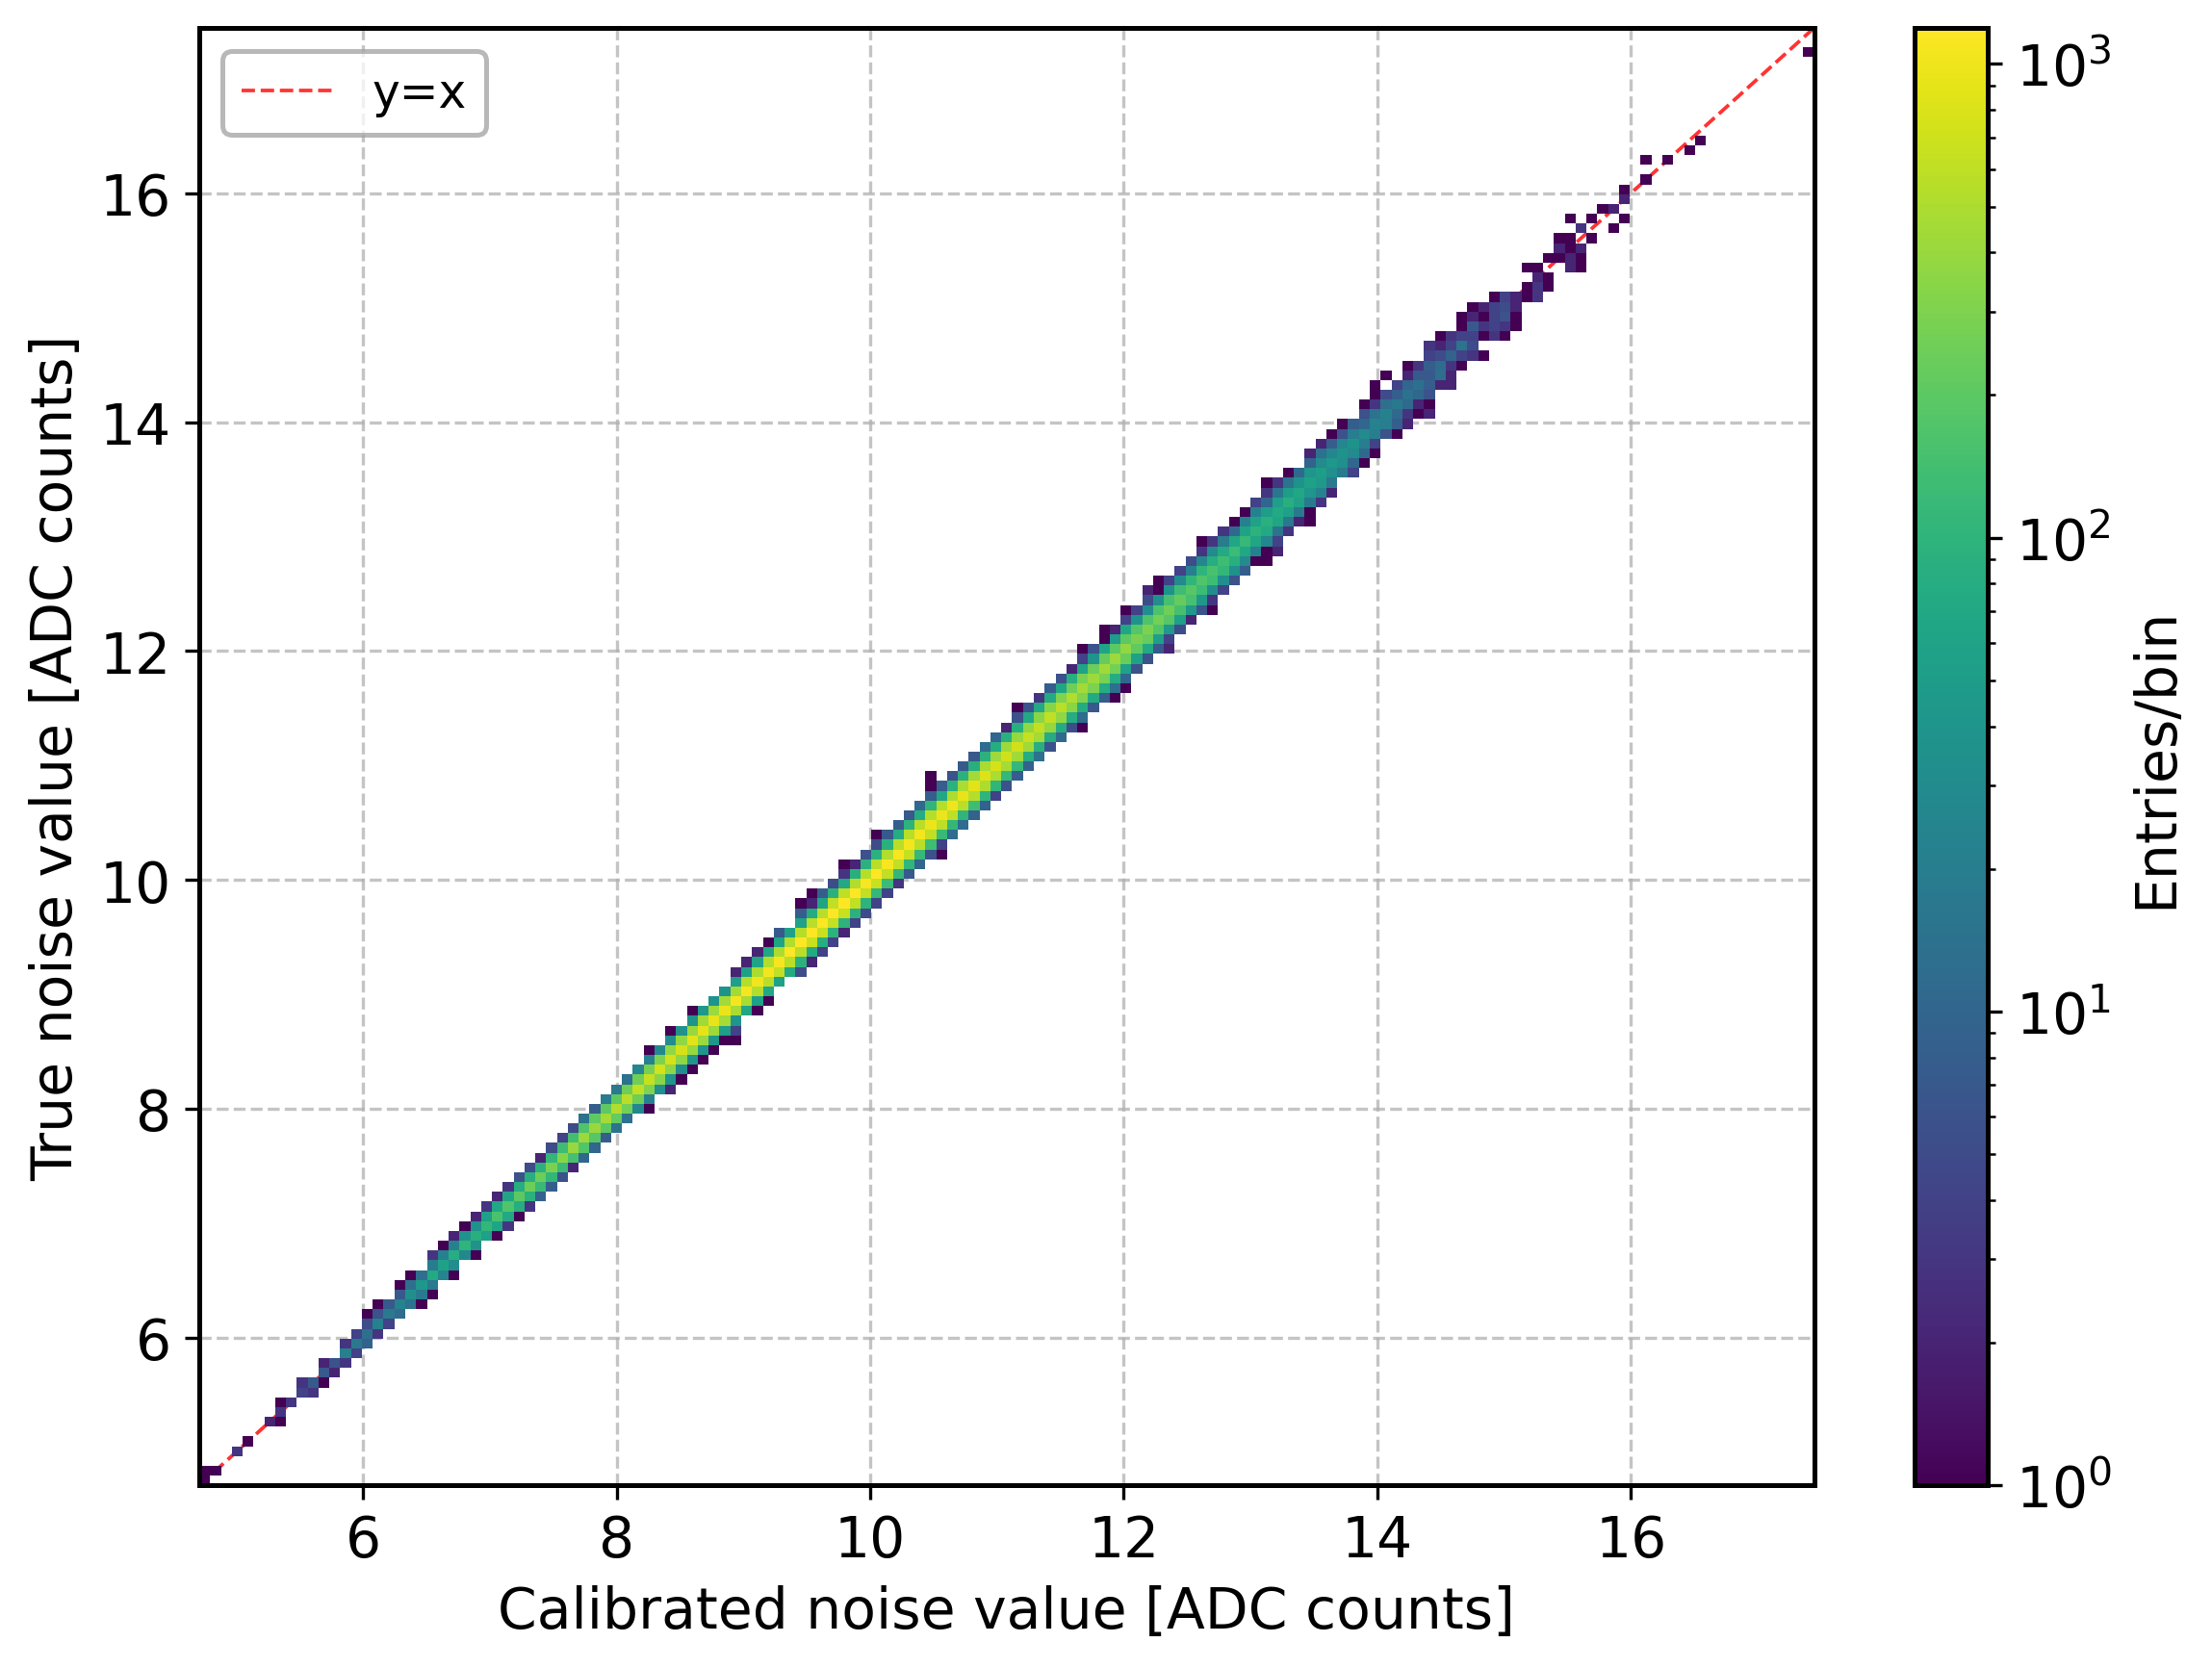
\includegraphics[width=0.49\linewidth]{figures/chapter4/calibration/noise_correlation}
    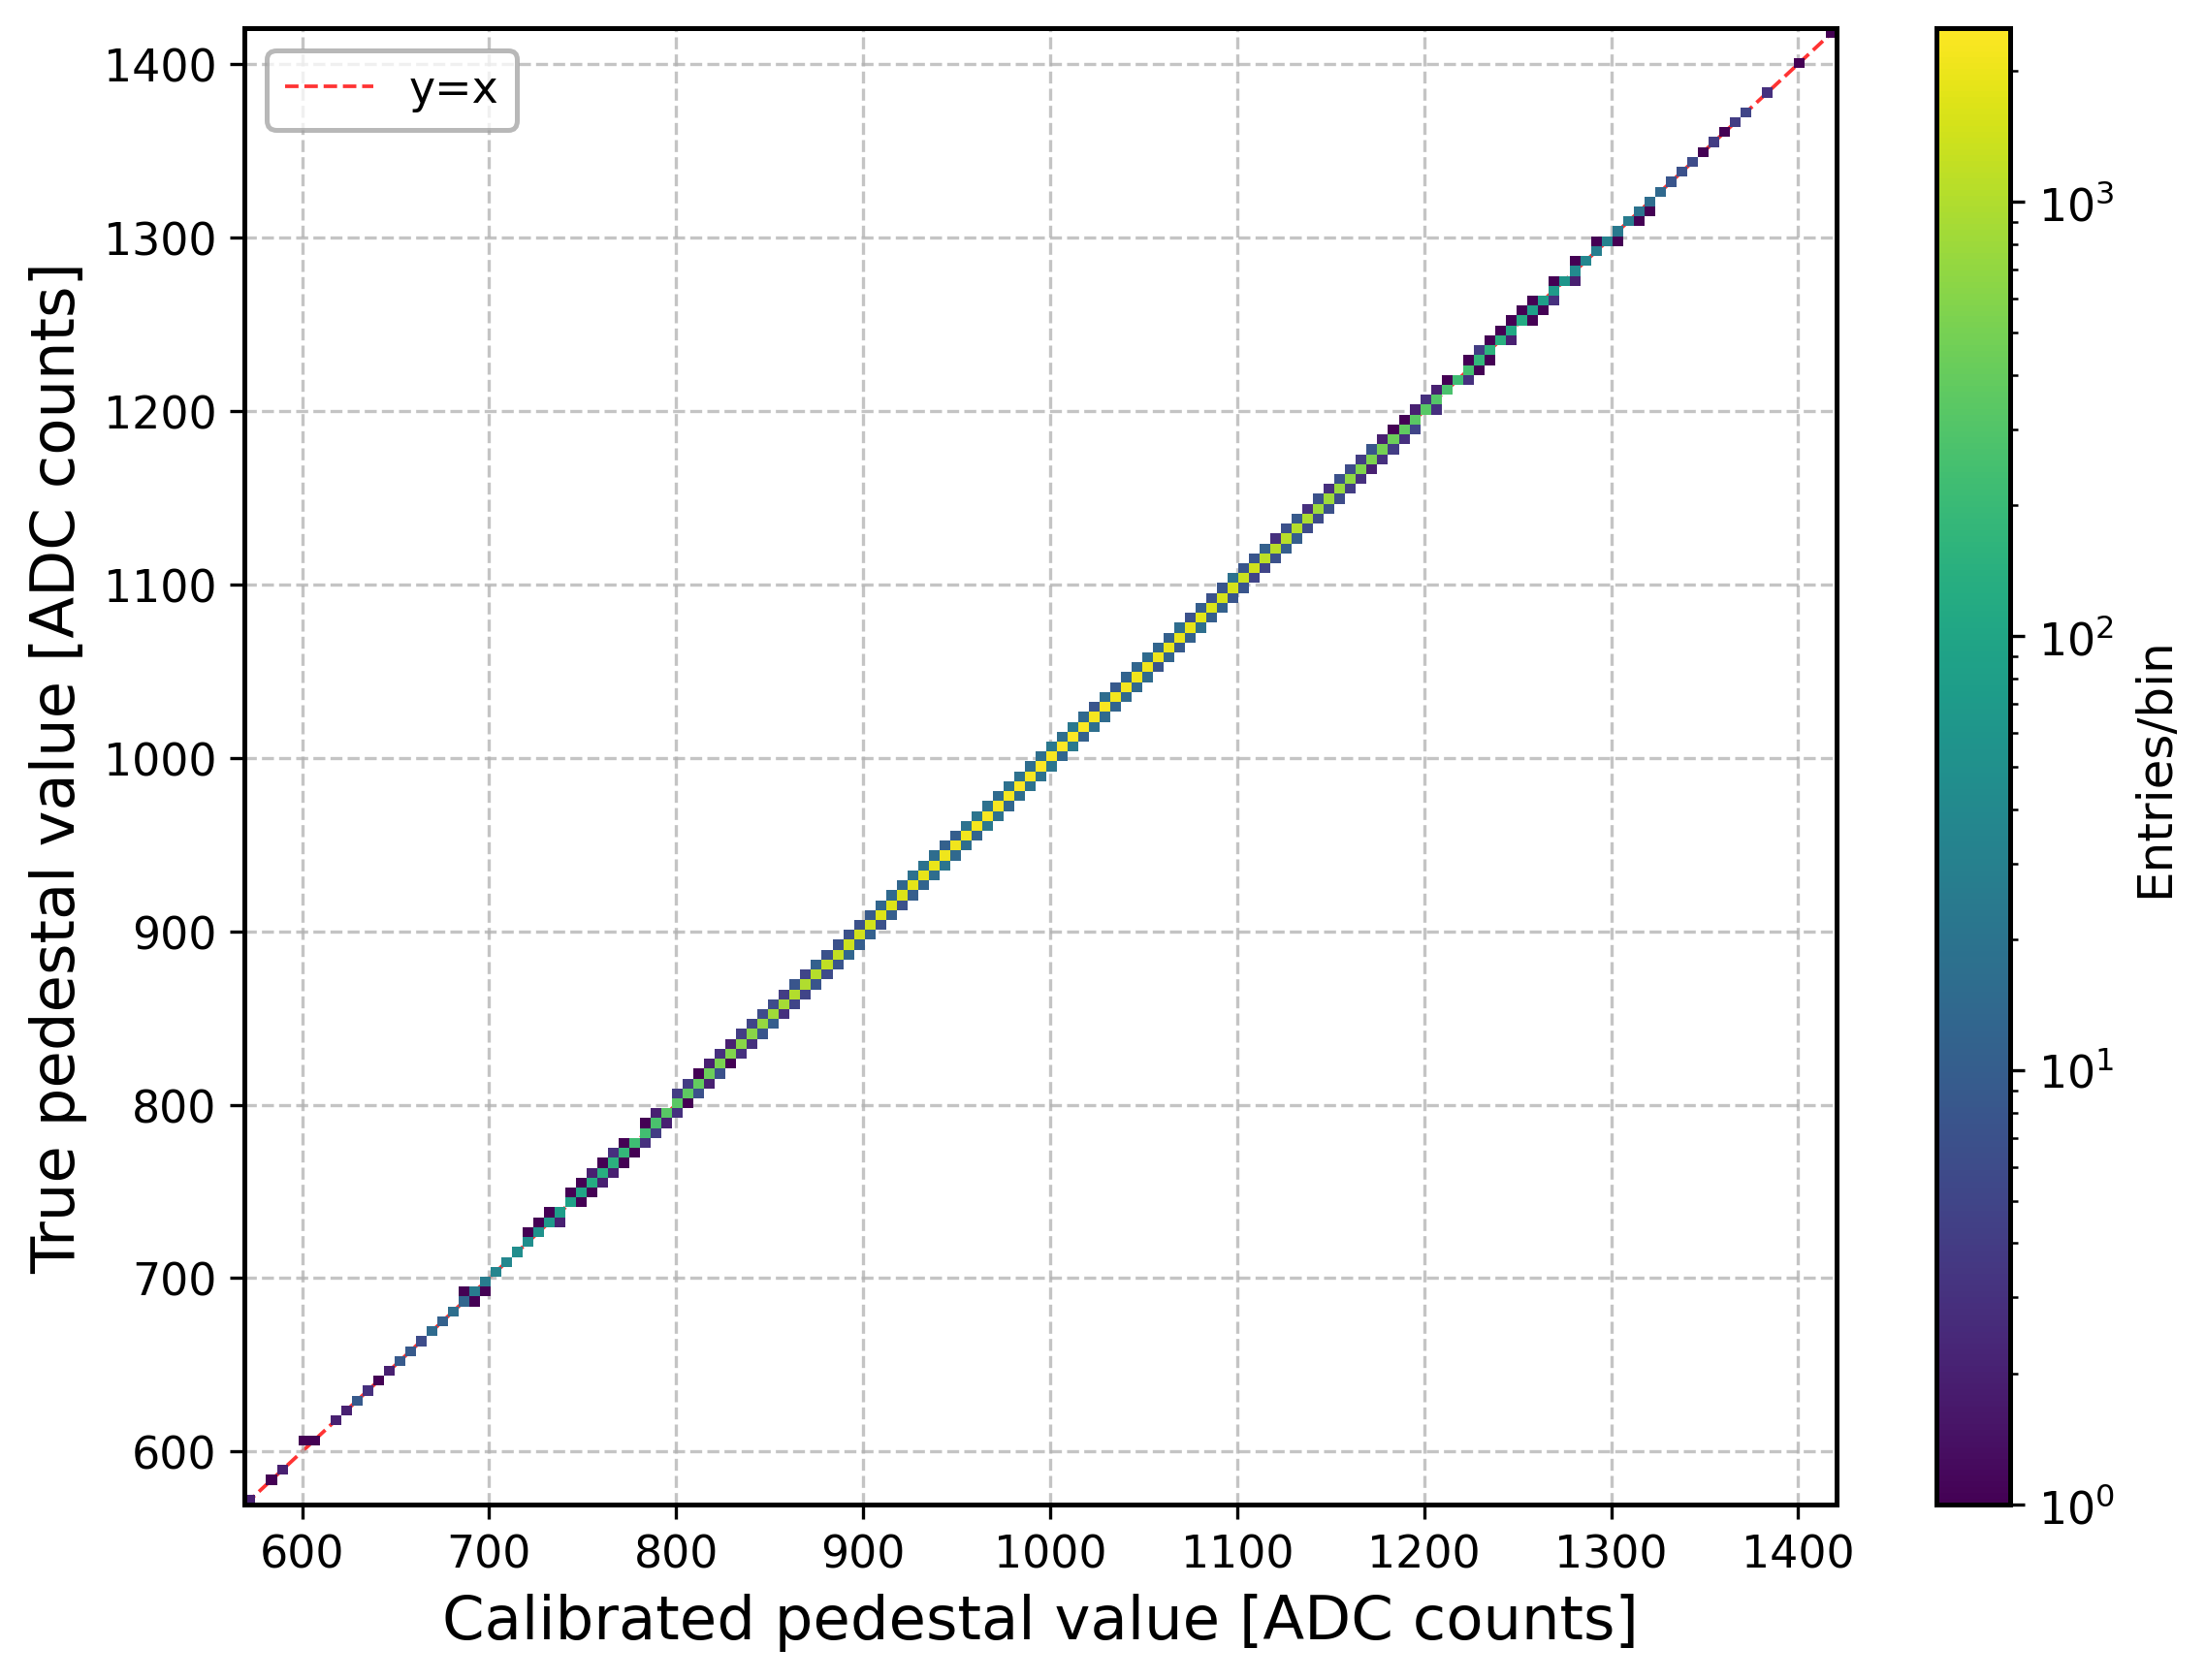
\includegraphics[width=0.49\linewidth]{figures/chapter4/calibration/pedestal_correlation}
    \caption{Two-dimensional correlation histograms between the true Monte Carlo values and the calibrated values for pixel noise (left) and pedestal levels (right). The red dashed line represents the ideal $y = x$ correlation.}
    \label{fig:noise_pedestal}
\end{figure}

Fig. \ref{fig:noise_distribution} shows the distribution of the calibrated values of the noise matrix and the residuals distribution. The ADC noise distribution is not a Gaussian because it is the product of two random variables, the ENC and gain, distributed according two different Gaussian distributions. The resulting distribution is a more complex skewed distribution, with mean equal to the product of the means of the parent distributions \cite{aroian1947}.

The residuals distribution has a standard deviation of about 0.07 ADC, equal to a mean relative error on the calibrated pixel value of 0.7\%, which is compatible with the expected relative error estimated from Eq. \ref{eq:noise_uncertainty} using the average number of events per pixel, which is about 11000 events.

Analogous results have been obtained for the pedestal calibration, whose residuals distribution has a standard deviation of 0.1 ADC, compatible with the expected value estimated from Eq. \ref{eq:noise_uncertainty}.

\begin{figure}
    \centering
    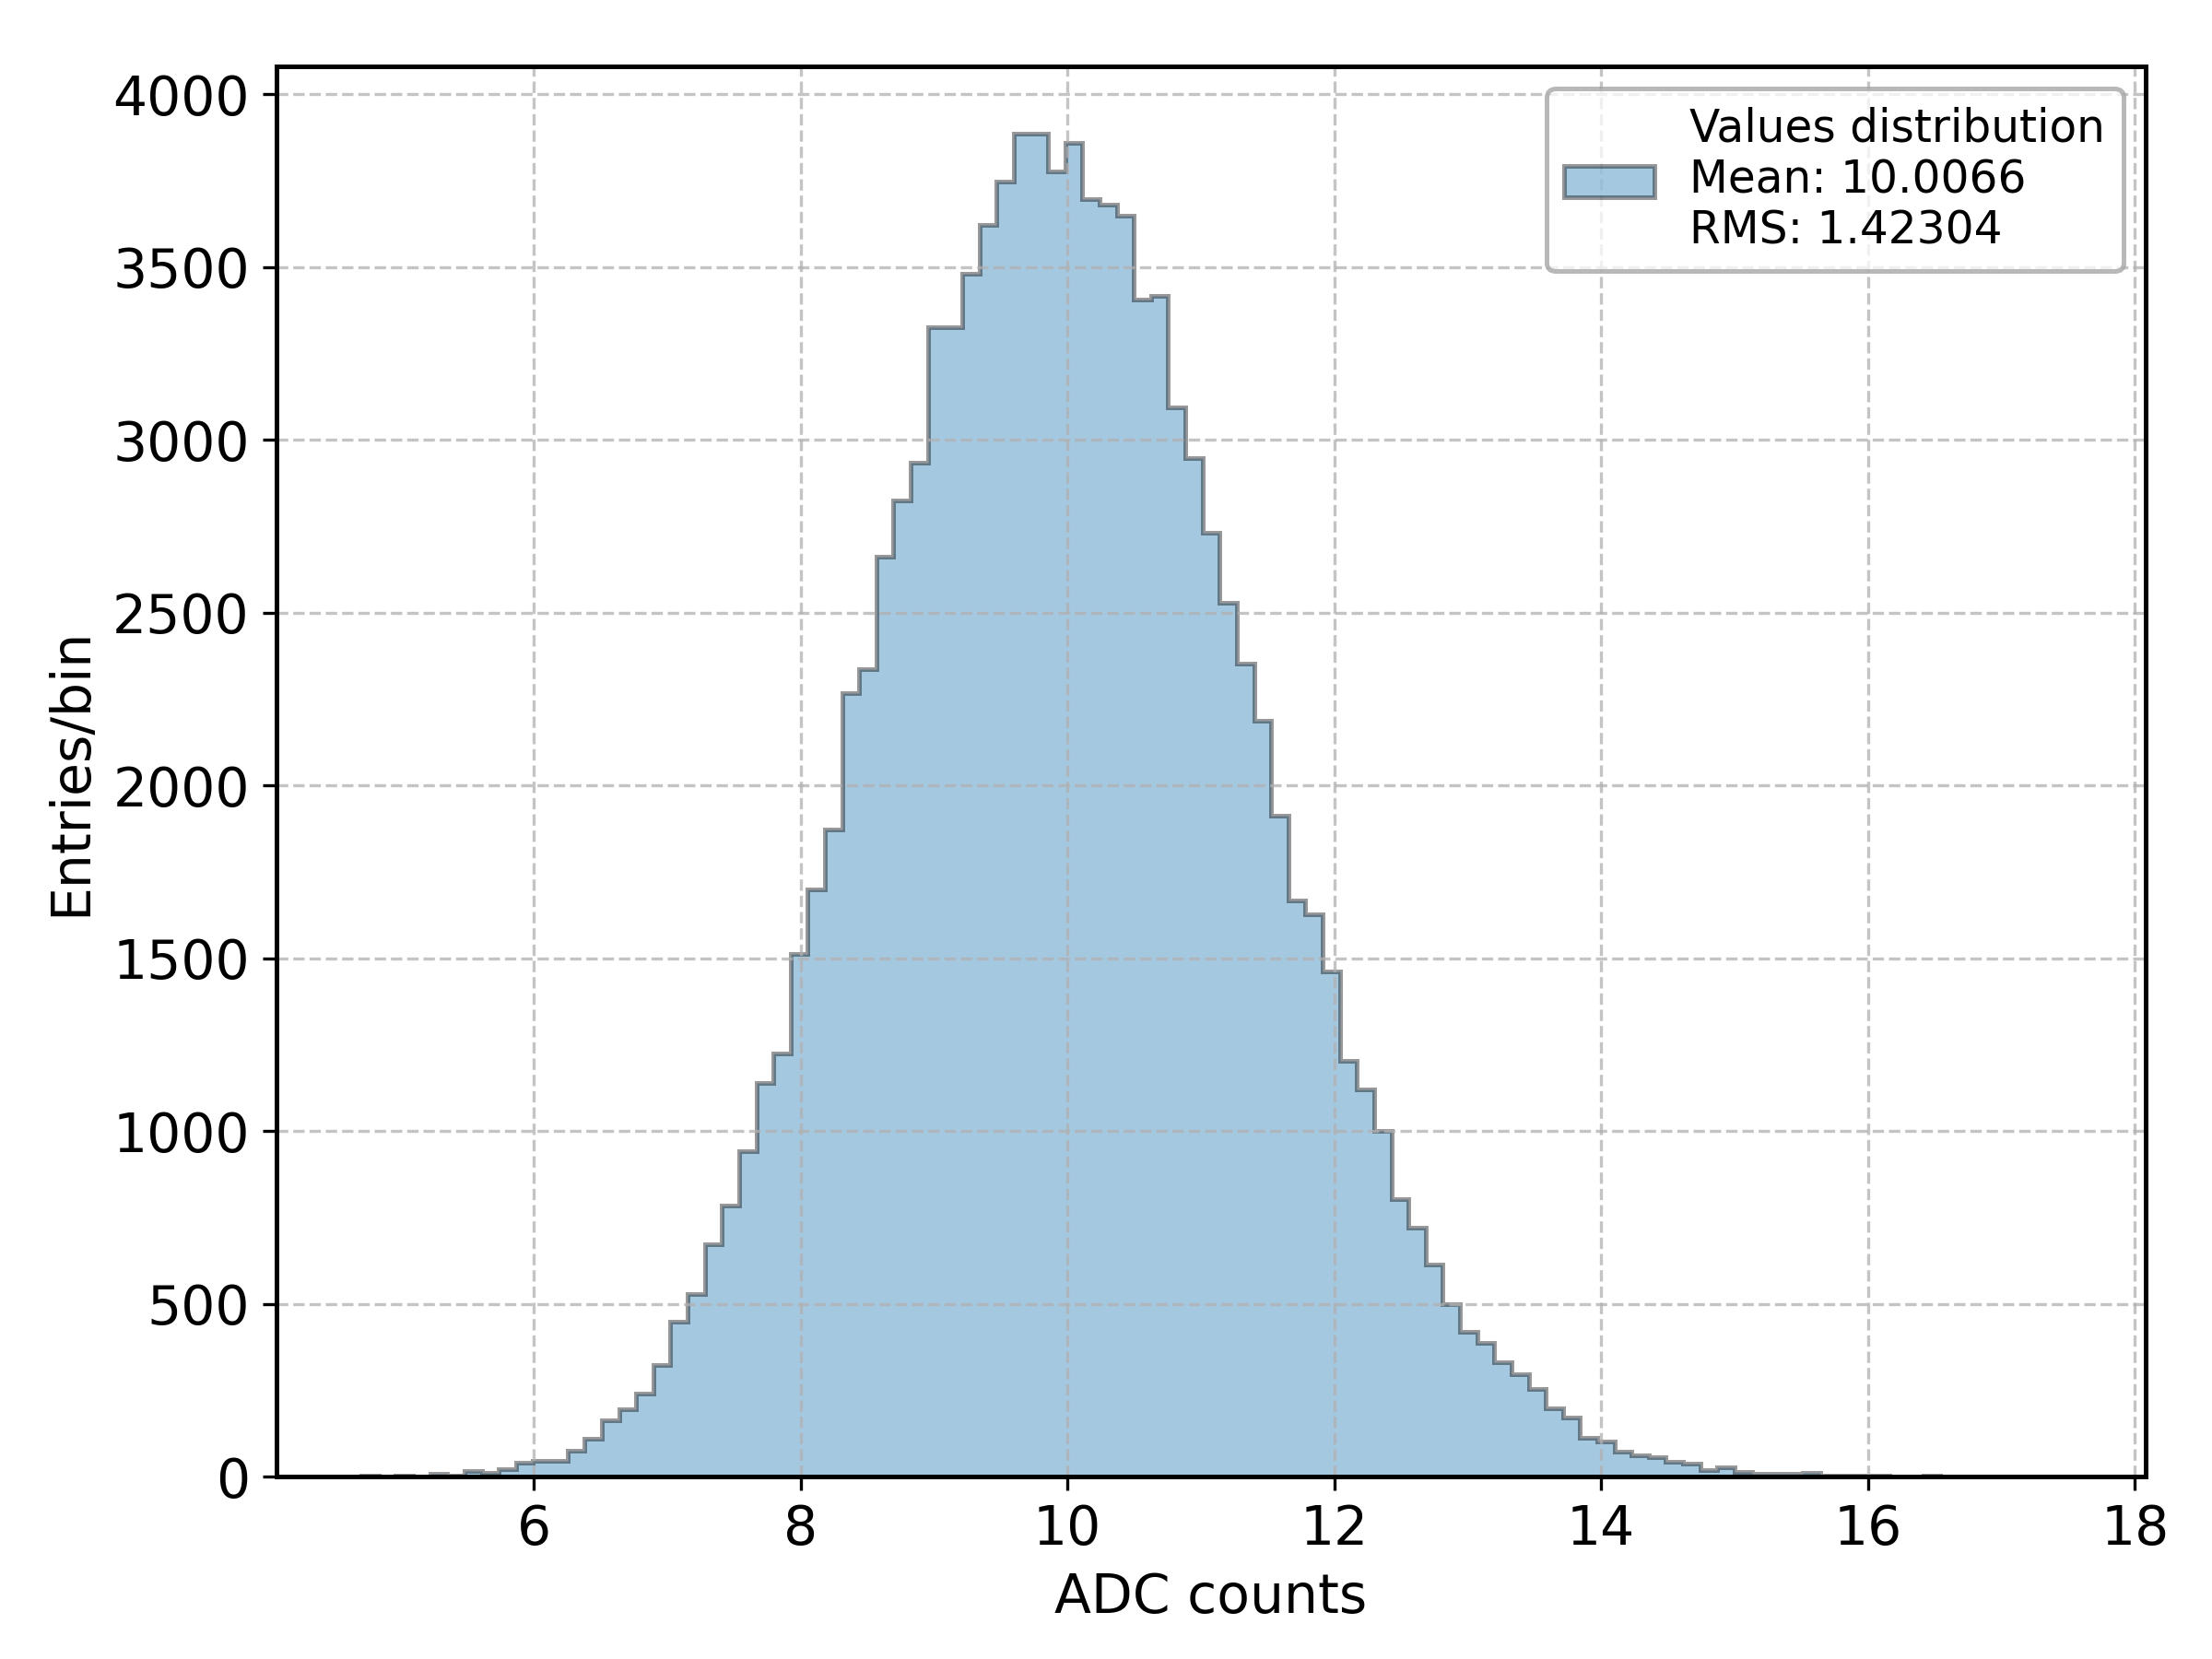
\includegraphics[width=0.49\linewidth]{figures/chapter4/noise_matrix_distribution}
    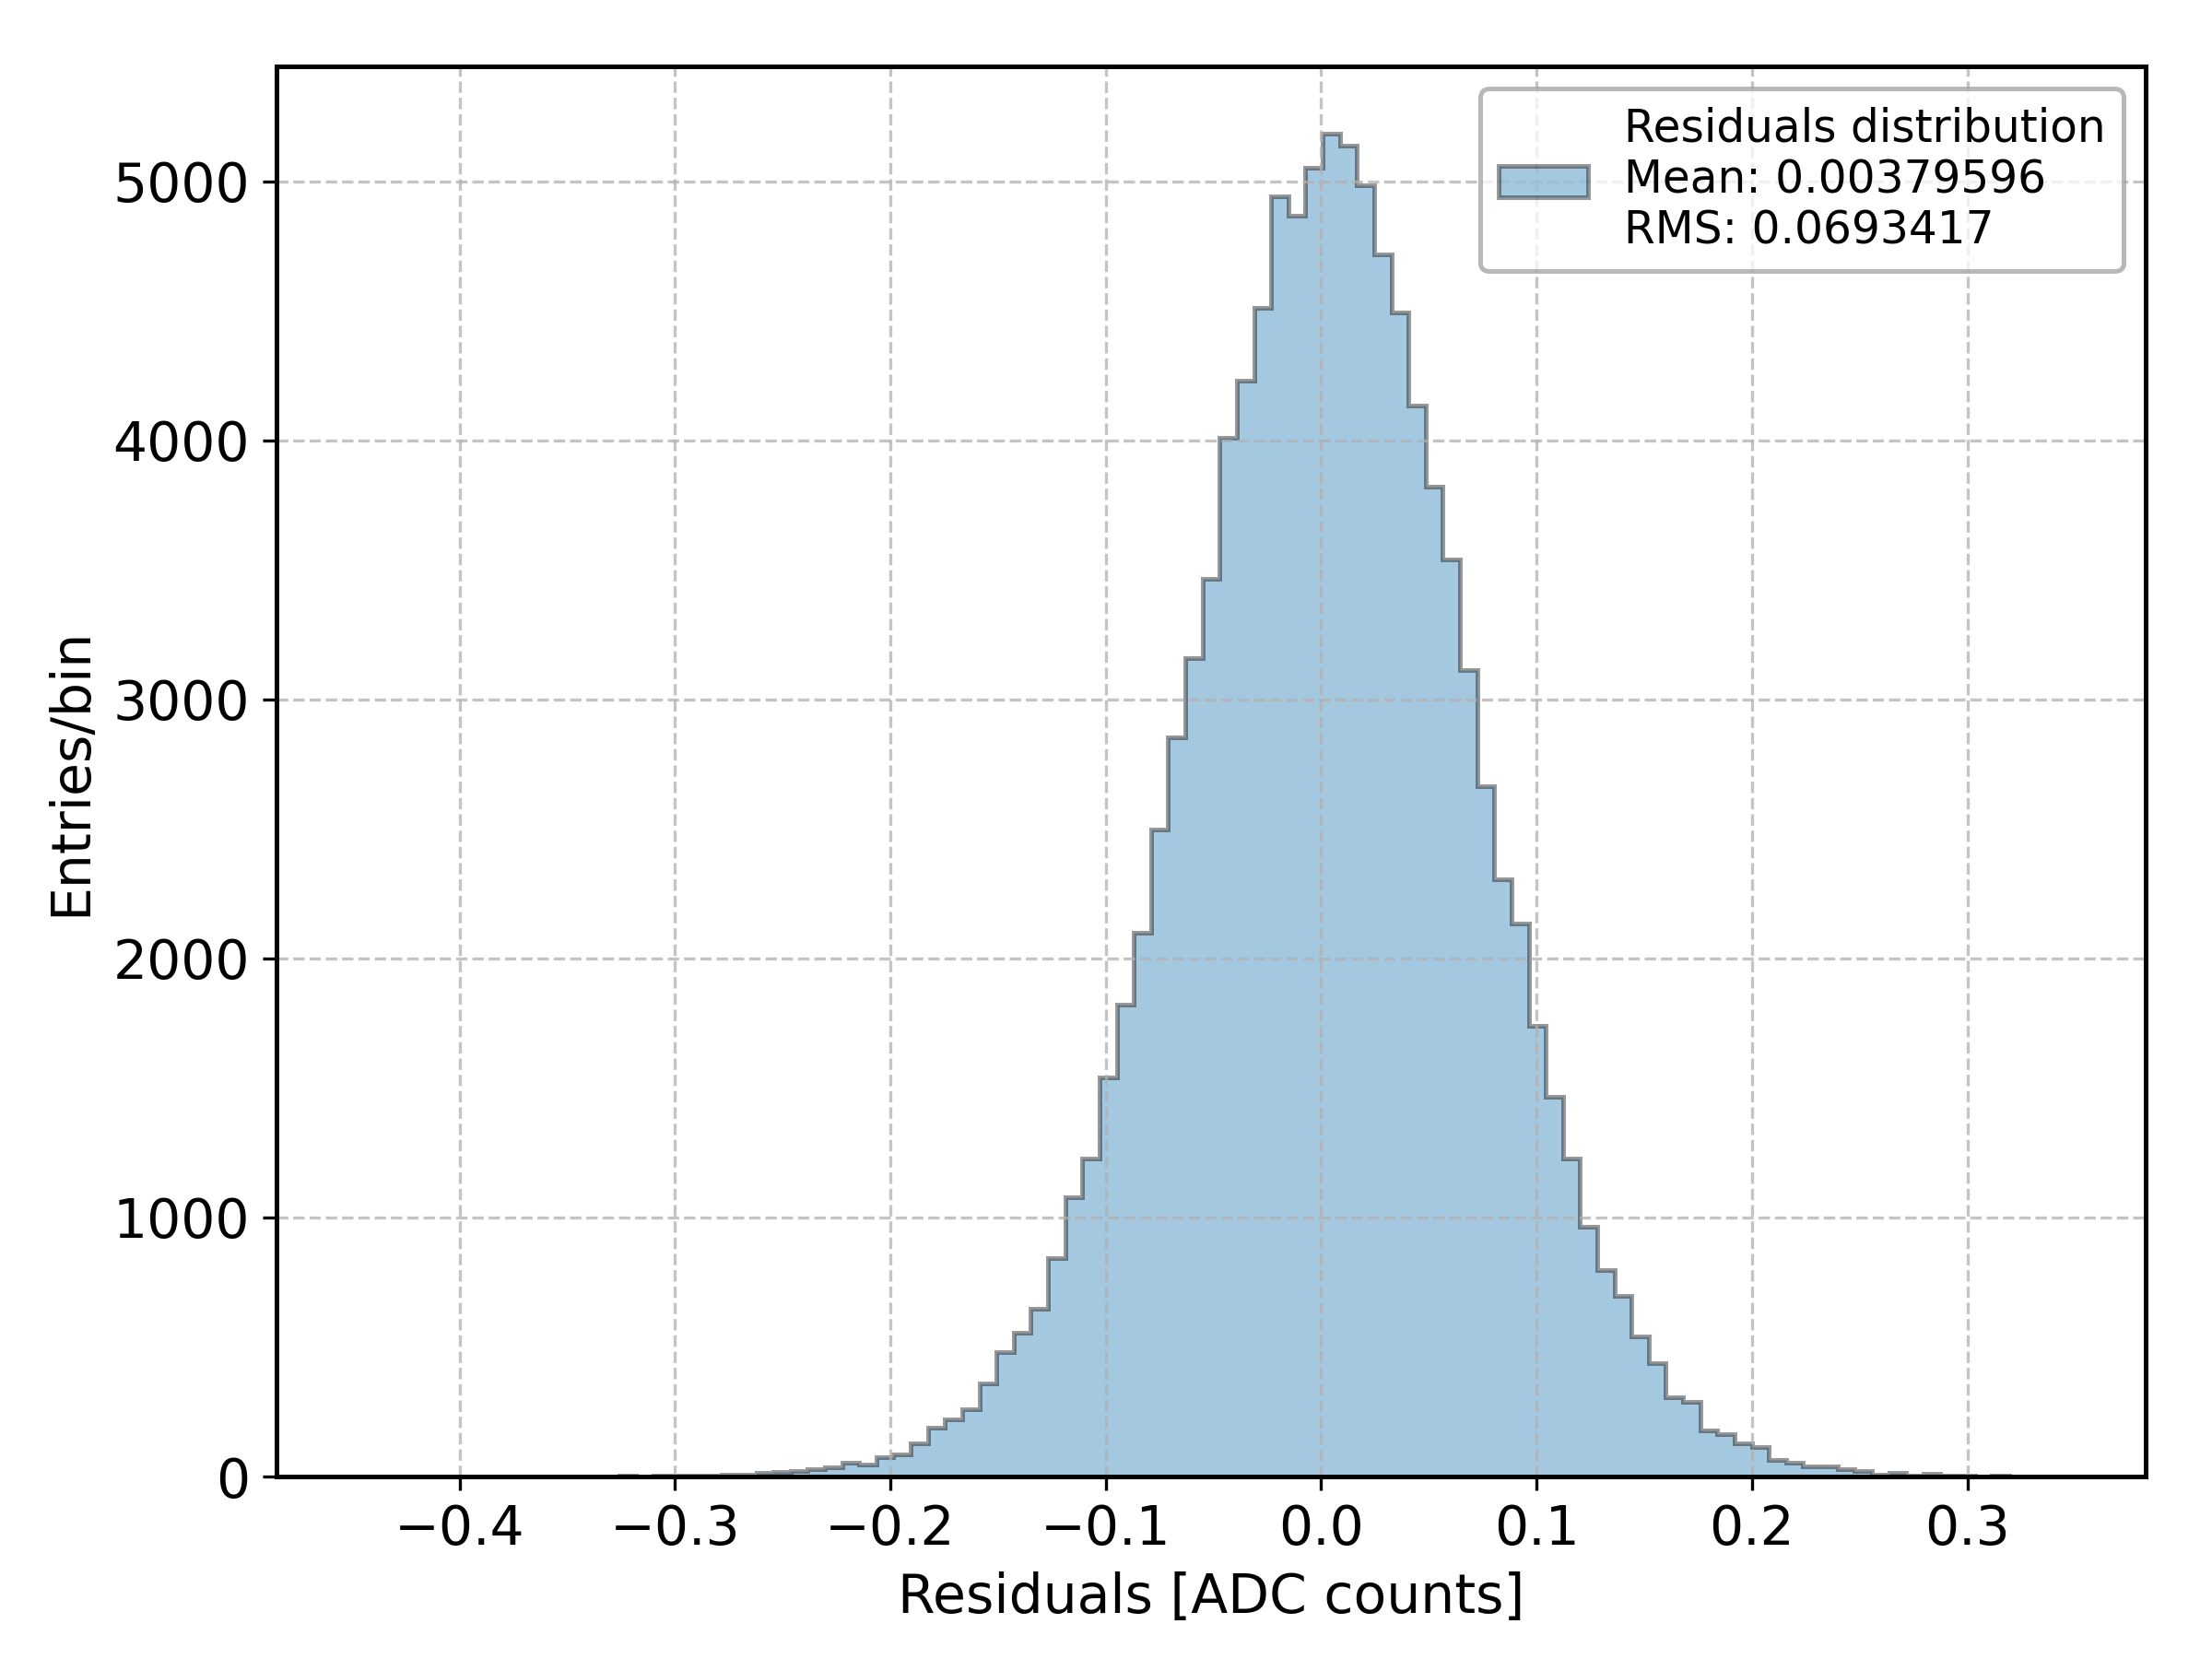
\includegraphics[width=0.49\linewidth]{figures/chapter4/noise_matrix_residuals}
    \caption{The left panel shows the calibrated values distribution of ADC noise, which is not a Gaussian distribution, but a distribution with a positive skewness. The residuals distribution is visible in the right panel.}
    \label{fig:noise_distribution}
\end{figure}

With these two calibration files, it is now possible to re-analyze the same dataset to calibrate the normalized gain. Both algorithms described above have been tested. The first one is straightforward, as it only requires using the noise and pedestal calibration products to remove offsets and correctly weight the pixel contents. However, with this method, only about 6\% of all events are classifiable as one-pixel events and can be used for the calibration, meaning that on average each pixel collects only about 6 events.

The second method requires running a simulation of the source spectrum using the noise and pedestal calibration products and assuming a uniform gain across the chip (the exact value is relevant only for the absolute gain; thus, for the normalized gain, it can be set to 1). The simulated dataset is then reconstructed, and the resulting spectrum is used as the probability density function for the likelihood estimation of the normalized gain. This method exploits all events, resulting in an average of about 230 events per pixel.

The correlation between the true and the calibrated values of the normalized gain for the two methods is shown in Fig. \ref{fig:gain_results}. In both cases, the reconstructed values are well aligned along the $y=x$ identity line, demonstrating that both calibration procedures are unbiased and correctly reconstruct the normalized gain.

However, the two distributions show significant differences in terms of dispersion. The first method, being limited to one-pixel events with an average of only $\approx 6$ events per pixel, exhibits a broader distribution around the diagonal due to larger statistical fluctuations. In contrast, the second method exploits the full event statistics, resulting in a substantially narrower correlation band and thus a higher precision in the gain estimation. A very small fraction of outliers can be observed in the second method near the axes, corresponding to pixels where the likelihood minimization did not converge optimally. From the distribution of the residuals, the relative error on the normalized gain is found to be about 2\% for the first method and 1\% for the second method.

\begin{figure}
    \centering
    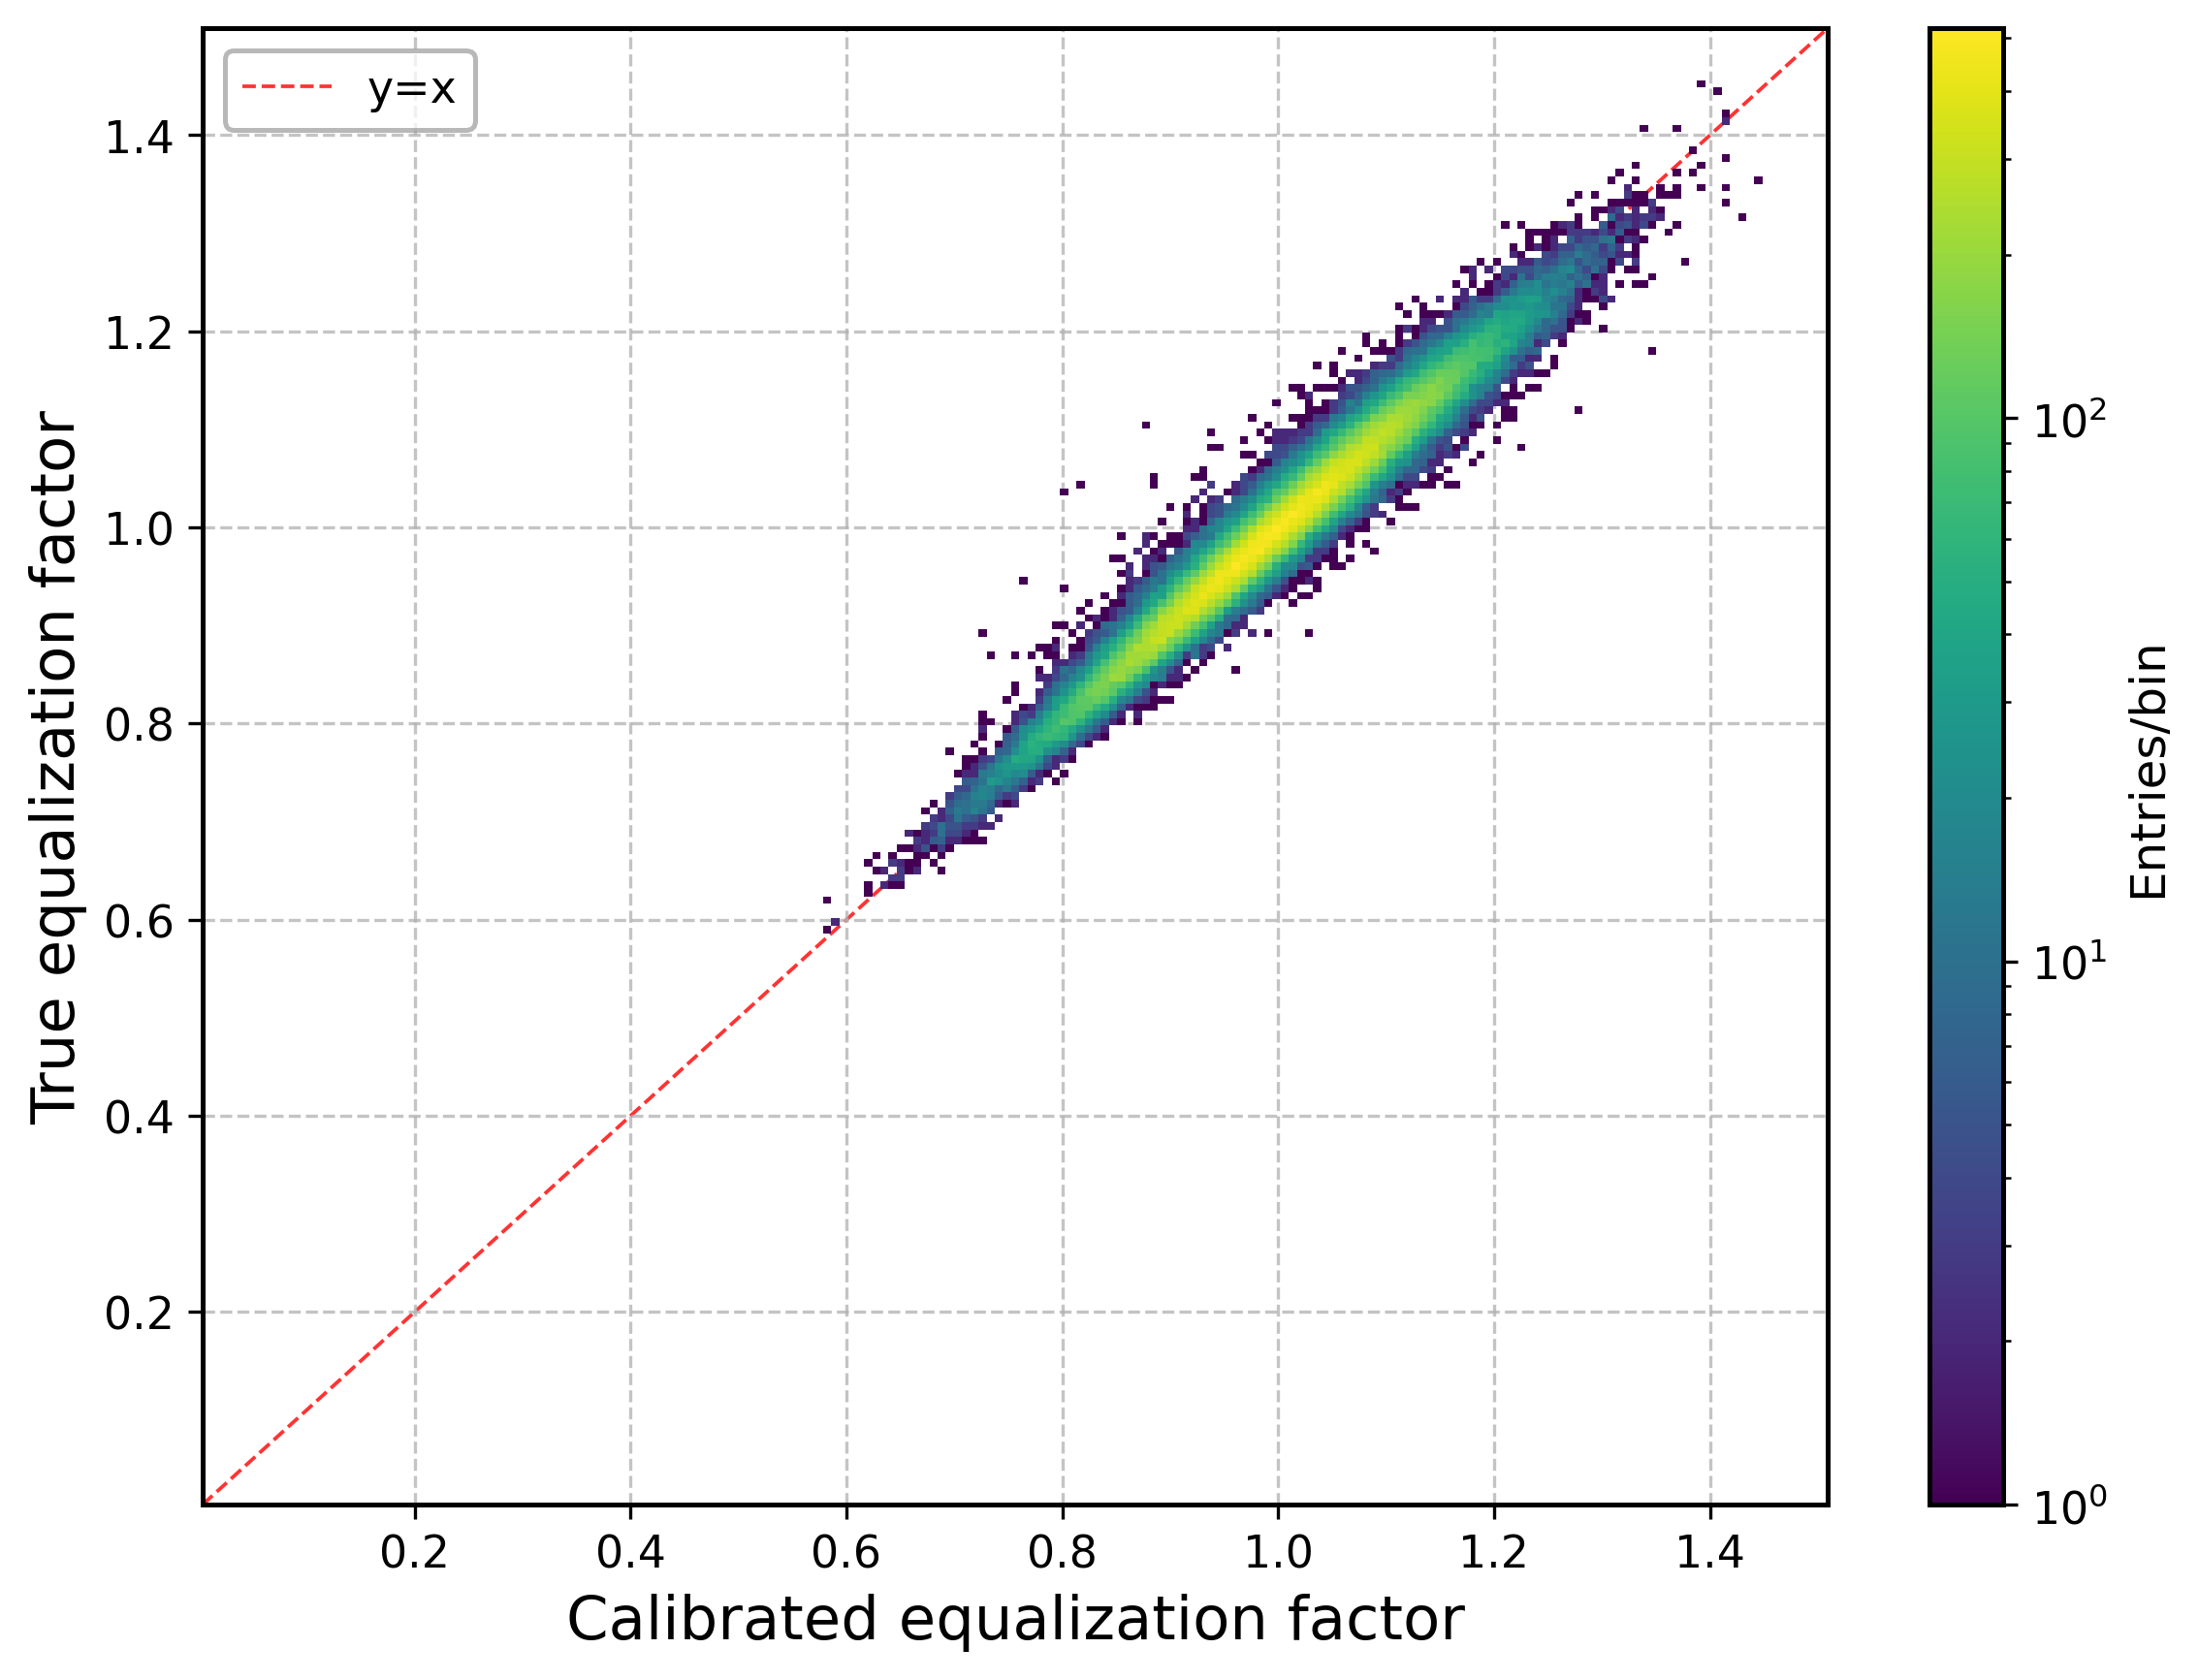
\includegraphics[width=0.49\linewidth]{figures/chapter4/calibration/equalization_correlation_method1}
    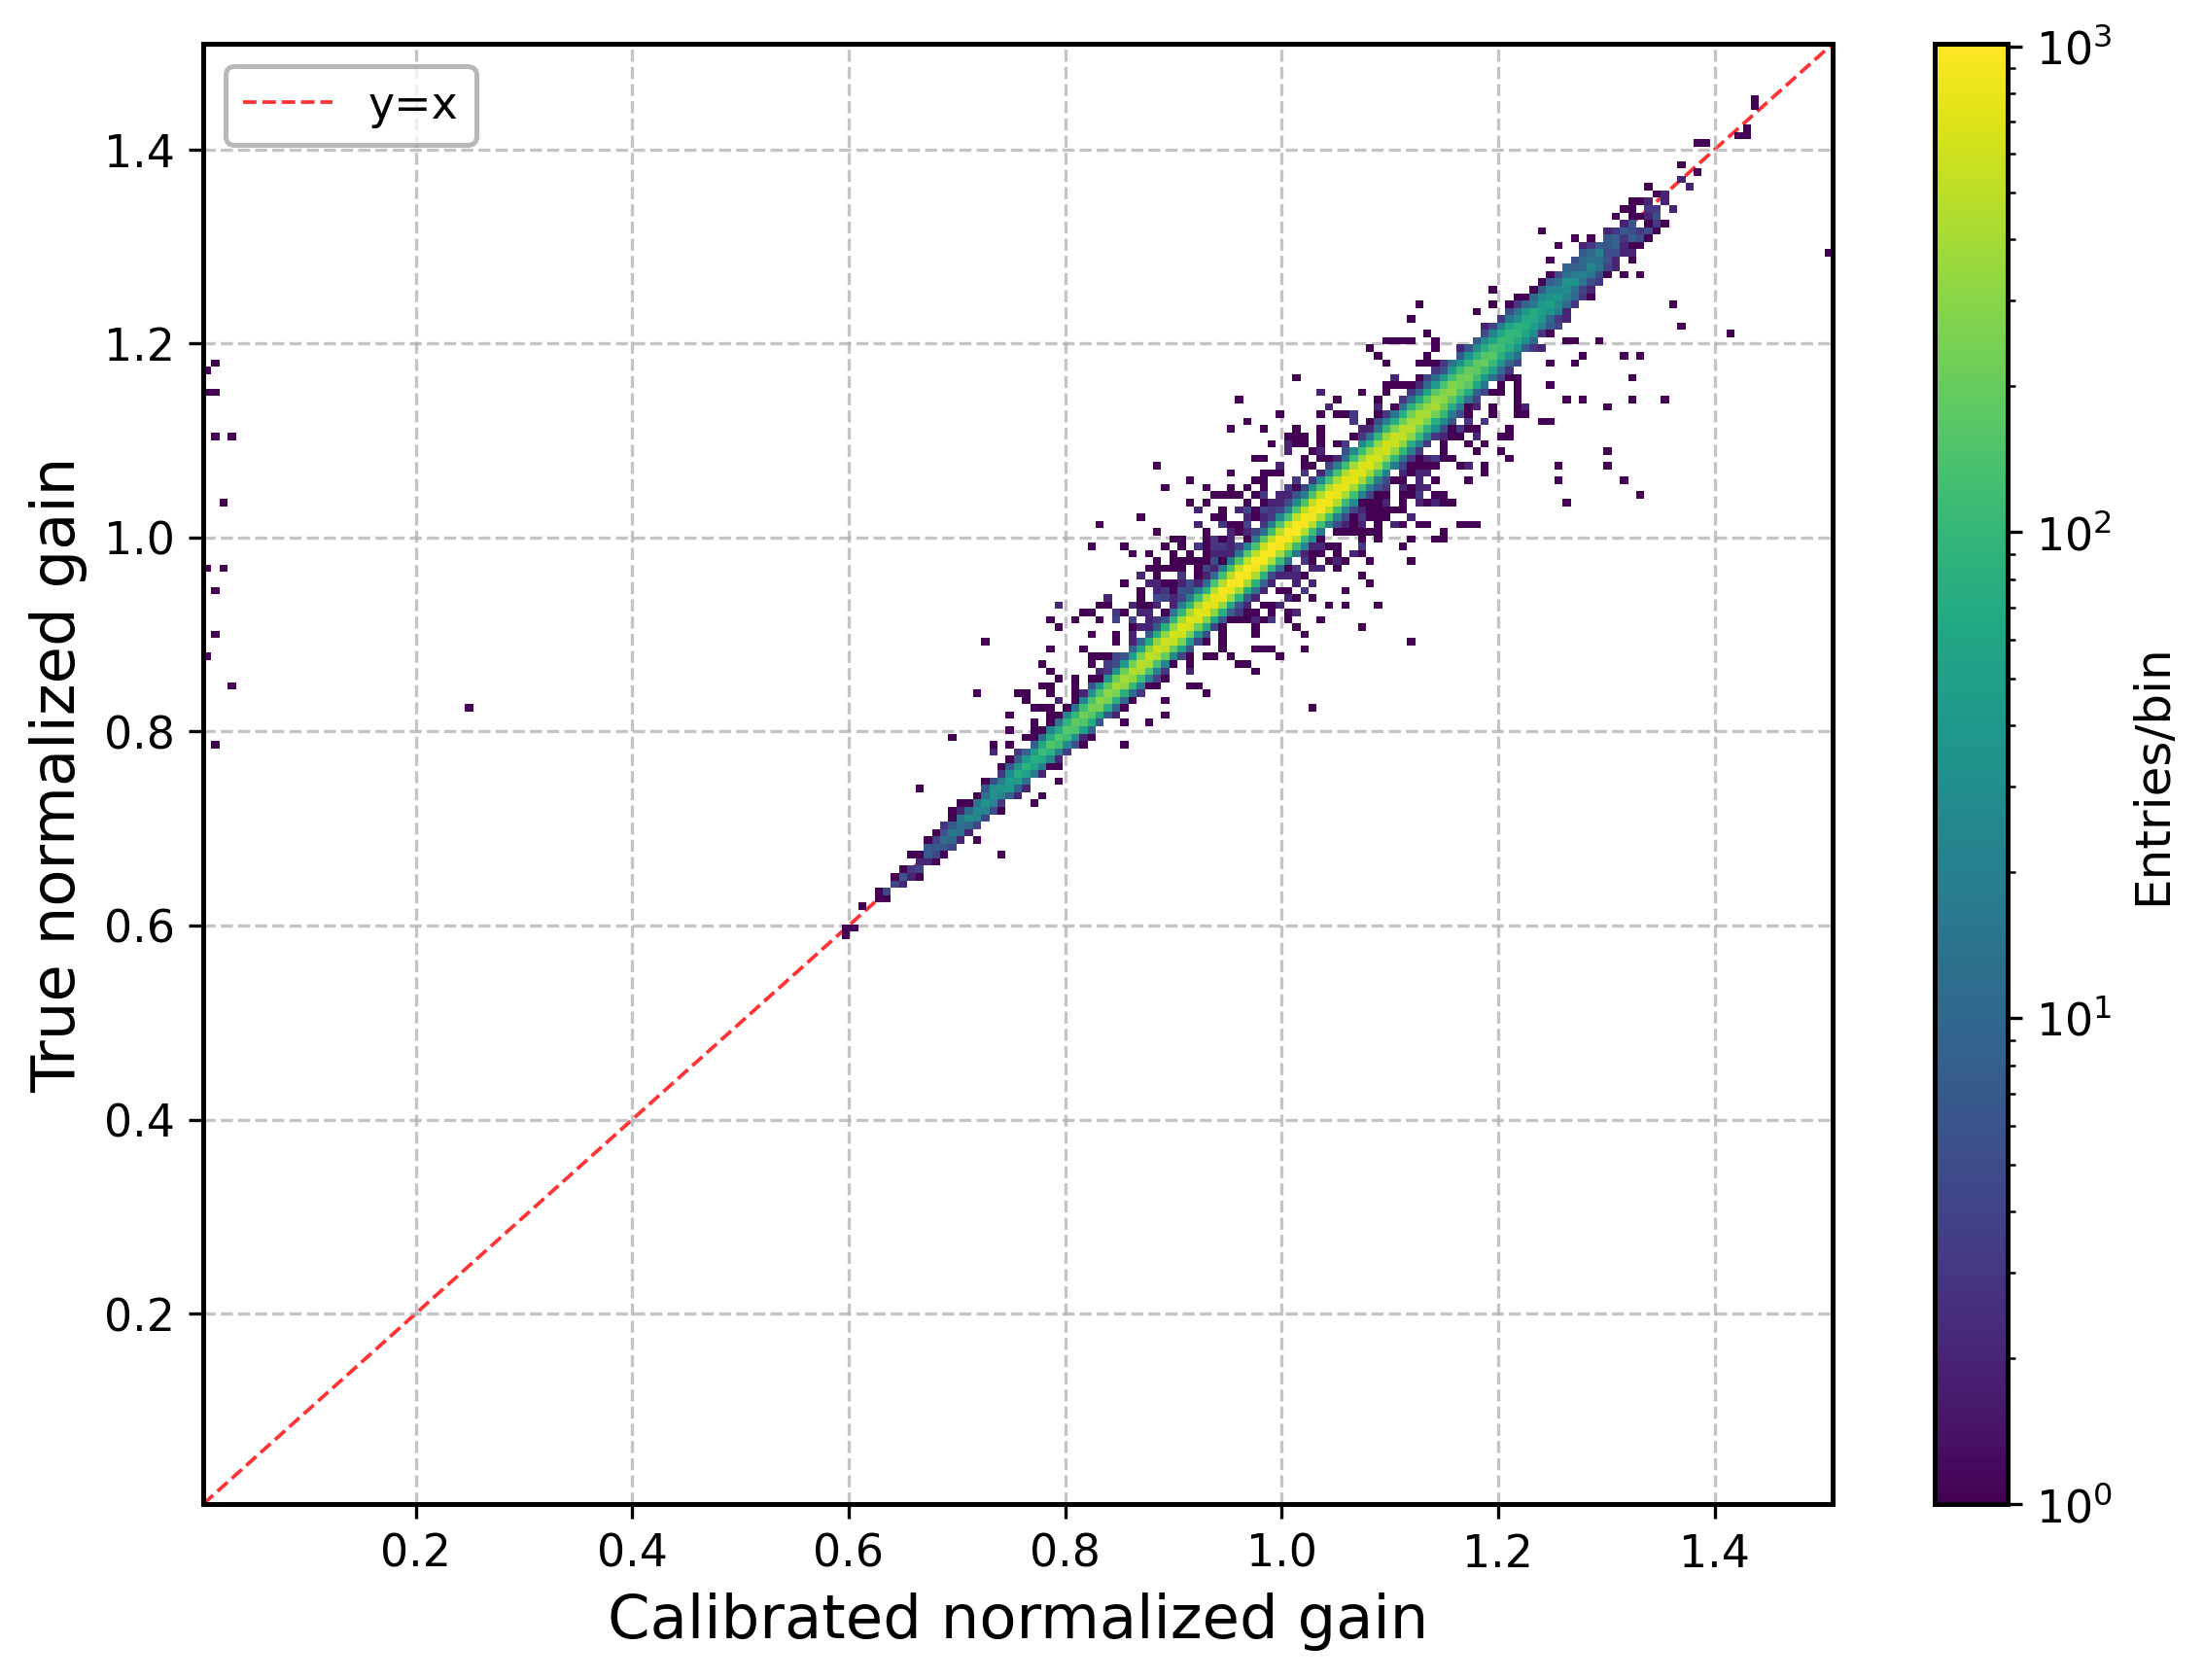
\includegraphics[width=0.49\linewidth]{figures/chapter4/calibration/equalization_correlation_method2}
    \caption{Two-dimensional correlation histograms between the calibrated equalization factors and the Monte Carlo truth for the one-pixel method (left) and the spectrum likelihood method (right). The red dashed line indicates the ideal $y = x$ correlation.}
    \label{fig:gain_results}
\end{figure}

\section{Position reconstruction}

With all the necessary calibration products, it is possible to reconstruct all the information about the events. The important thing to take into account is that one of the features of ASIX is that the size of the diffused charge cloud is a bit smaller than a pixel, meaning that the average cluster size is quite small, as shown in Chap. \ref{sec:asix_design}. While this feature is essential for spectroscopy, in order to minimize the contribution of noise, it introduces the need of a careful analysis to reconstruct the incident position.

As a consequence, different algorithms have been developed and compared to determine which one achieves the best spatial resolution. To estimate the performance of these algorithms, two distinct methods can be employed. 

The first approach is typical for space applications, where a source with a known spatial profile, such as a point-like source, is used to directly compare the true incidence position with the reconstructed one. In this work, this method is implemented using the Monte Carlo ground truth. The metric used to gauge the spatial resolution is the encircled energy fraction (EEF). The EEF is the cumulative density function of the radial distance distribution between the true and the reconstructed positions \cite{longair2011}.

Usually, the EEF is calculated by integrating the Point Spread Function (PSF), which represents the response of a detector to a point-like source. In this case, given the availability of the Monte Carlo ground truth positions, it can be directly derived from the radial residuals distribution. Common metrics of the EEF are the radii corresponding to 50\% (Half-Energy Width, HEW) and 90\% encircled energy, which represent the customary standard for space telescopes. The HEW measures the core spatial resolution, while the latter is sensitive to the extended tails of the distribution.

The second approach is standard in medical and industrial imaging and relies on evaluating the spatial response of the detector to an illuminated slit or a sharp edge. This method has been adopted to analyze laboratory experimental data.

\subsection{Charge barycenter}
\label{subsec:barycenter}

The simplest possible algorithm consists of calculating the barycenter of the pixels centers by weighting their positions with the collected charge

\begin{equation}
x = \frac{\sum_i x_i \cdot q_i}{\sum_i q_i}, \quad y = \frac{\sum_i y_i \cdot q_i}{\sum_i q_i},
\end{equation}
where $x_i$ and $y_i$ are the coordinates of the $i$-th pixel and $q_i$ is the charge collected by it.

\begin{figure}[!b]
    \centering
    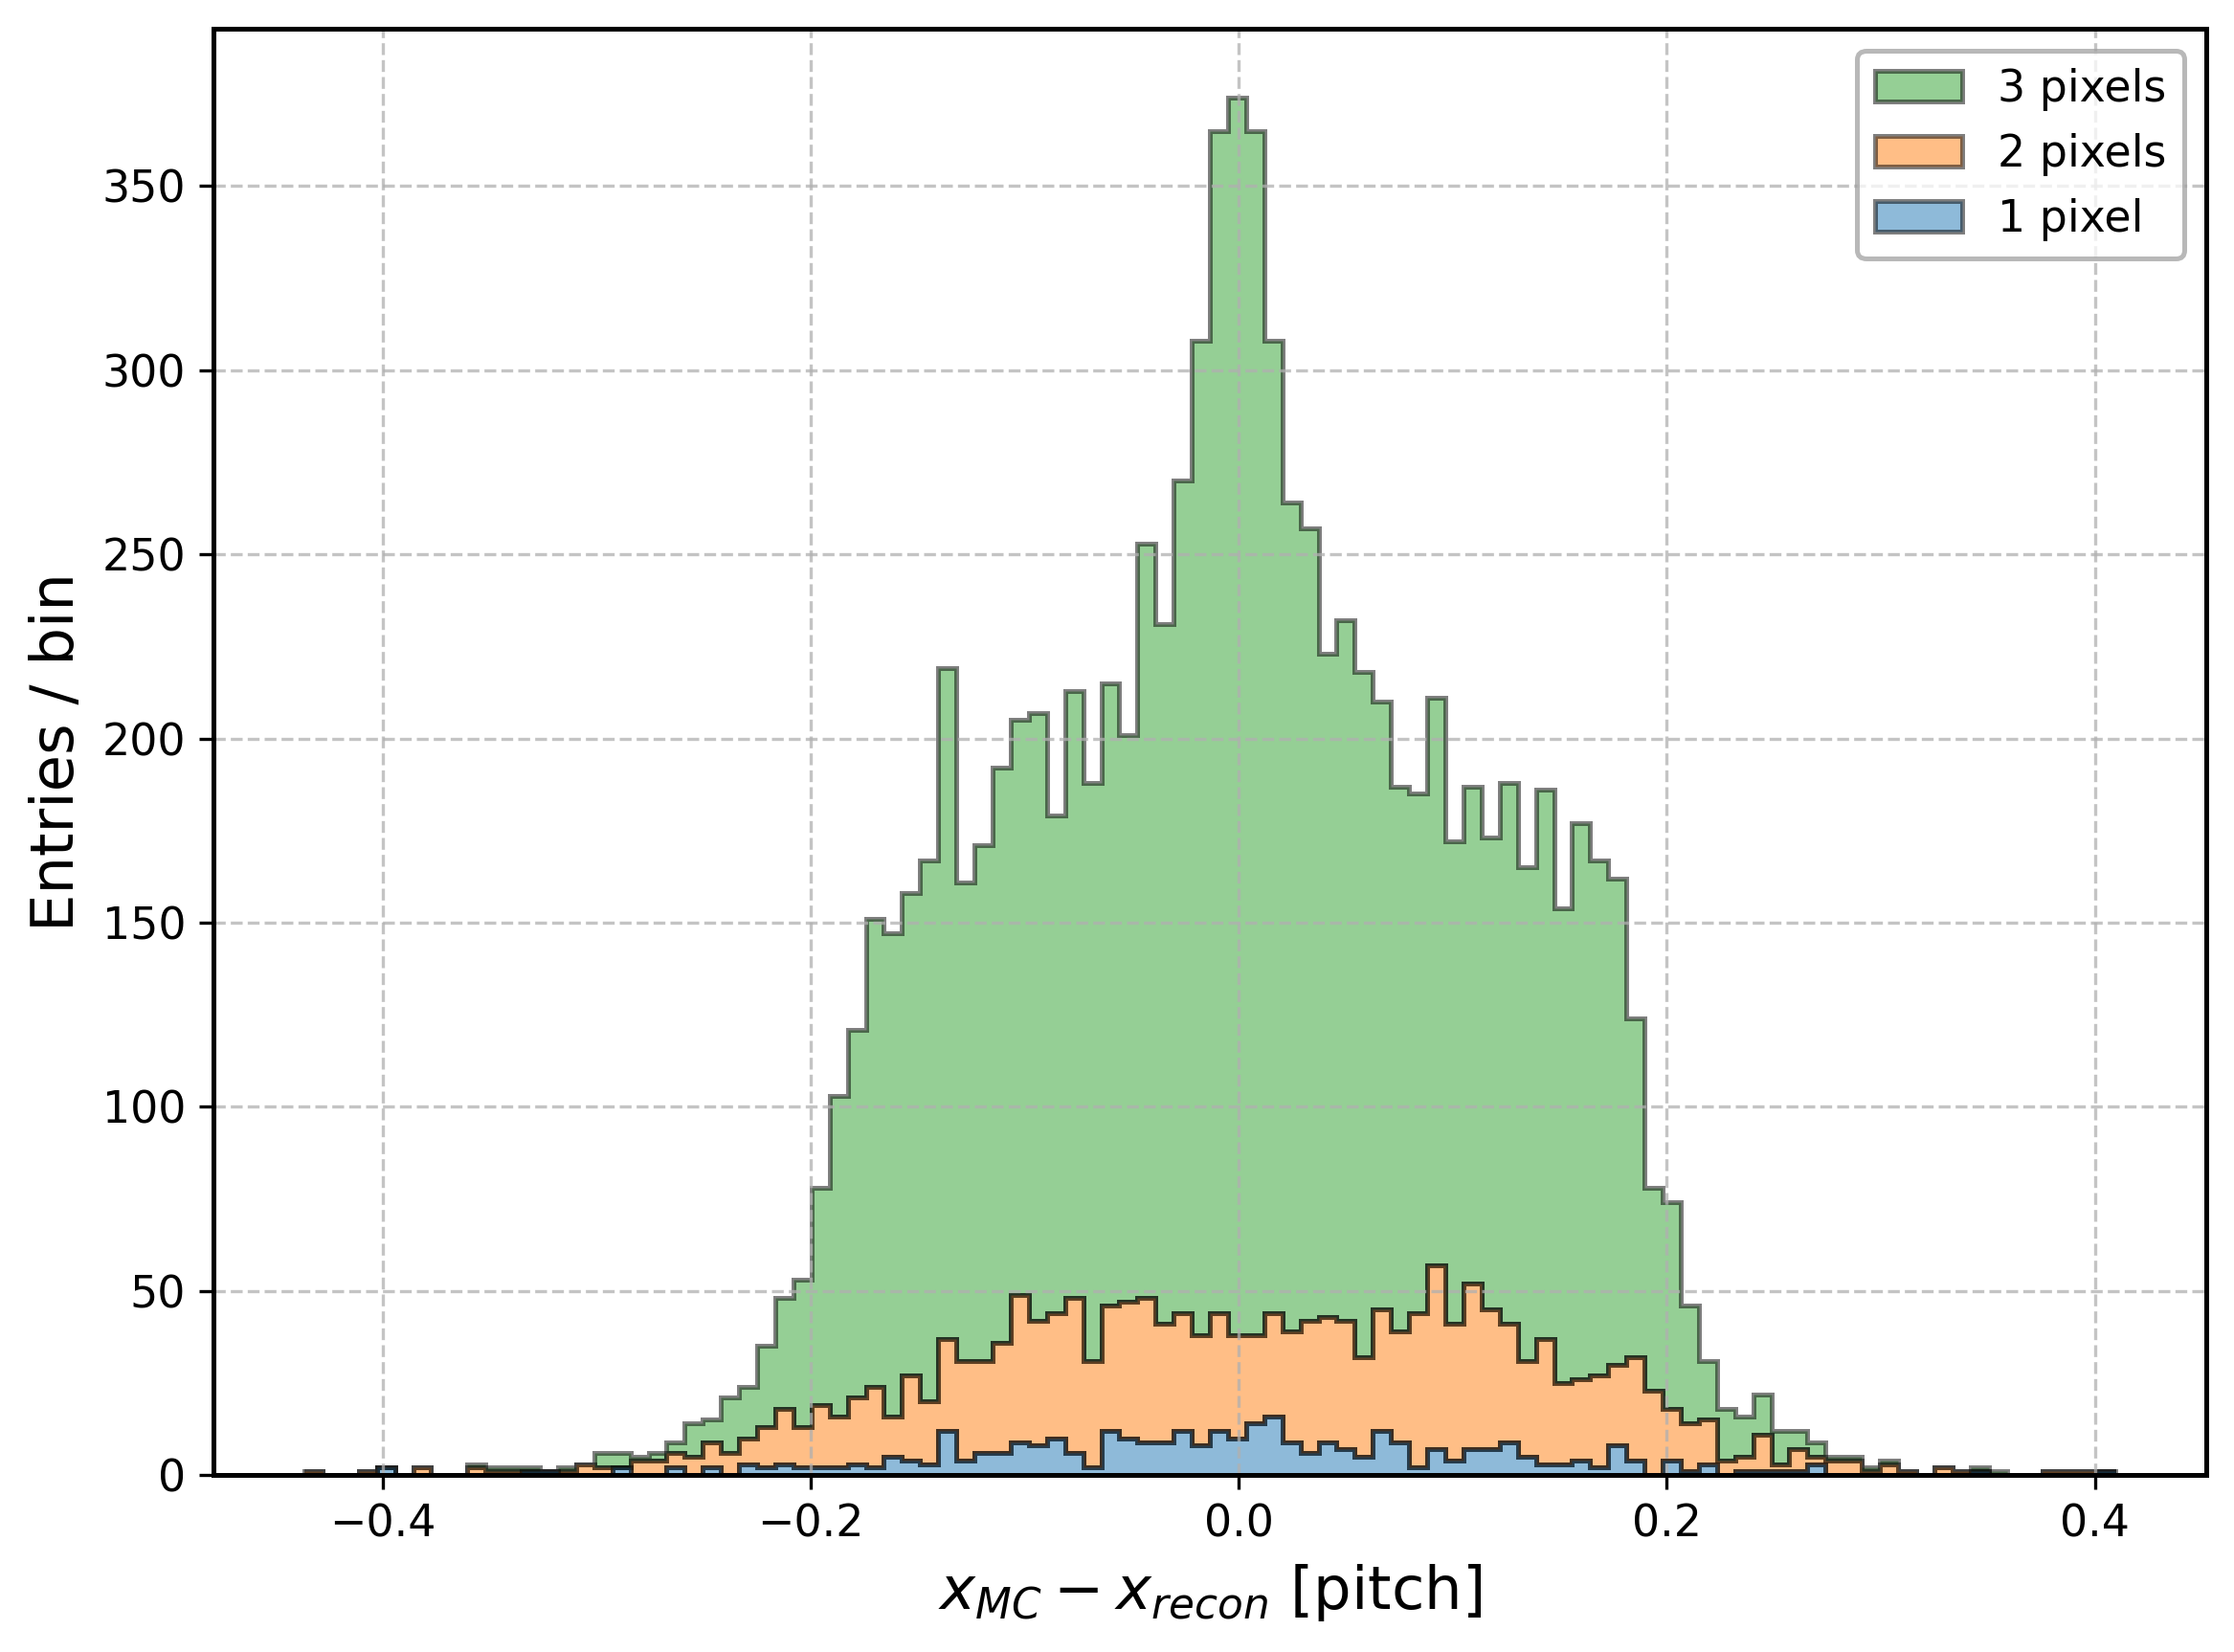
\includegraphics[width=0.49\linewidth]{figures/chapter4/position/barycenter_dx}
    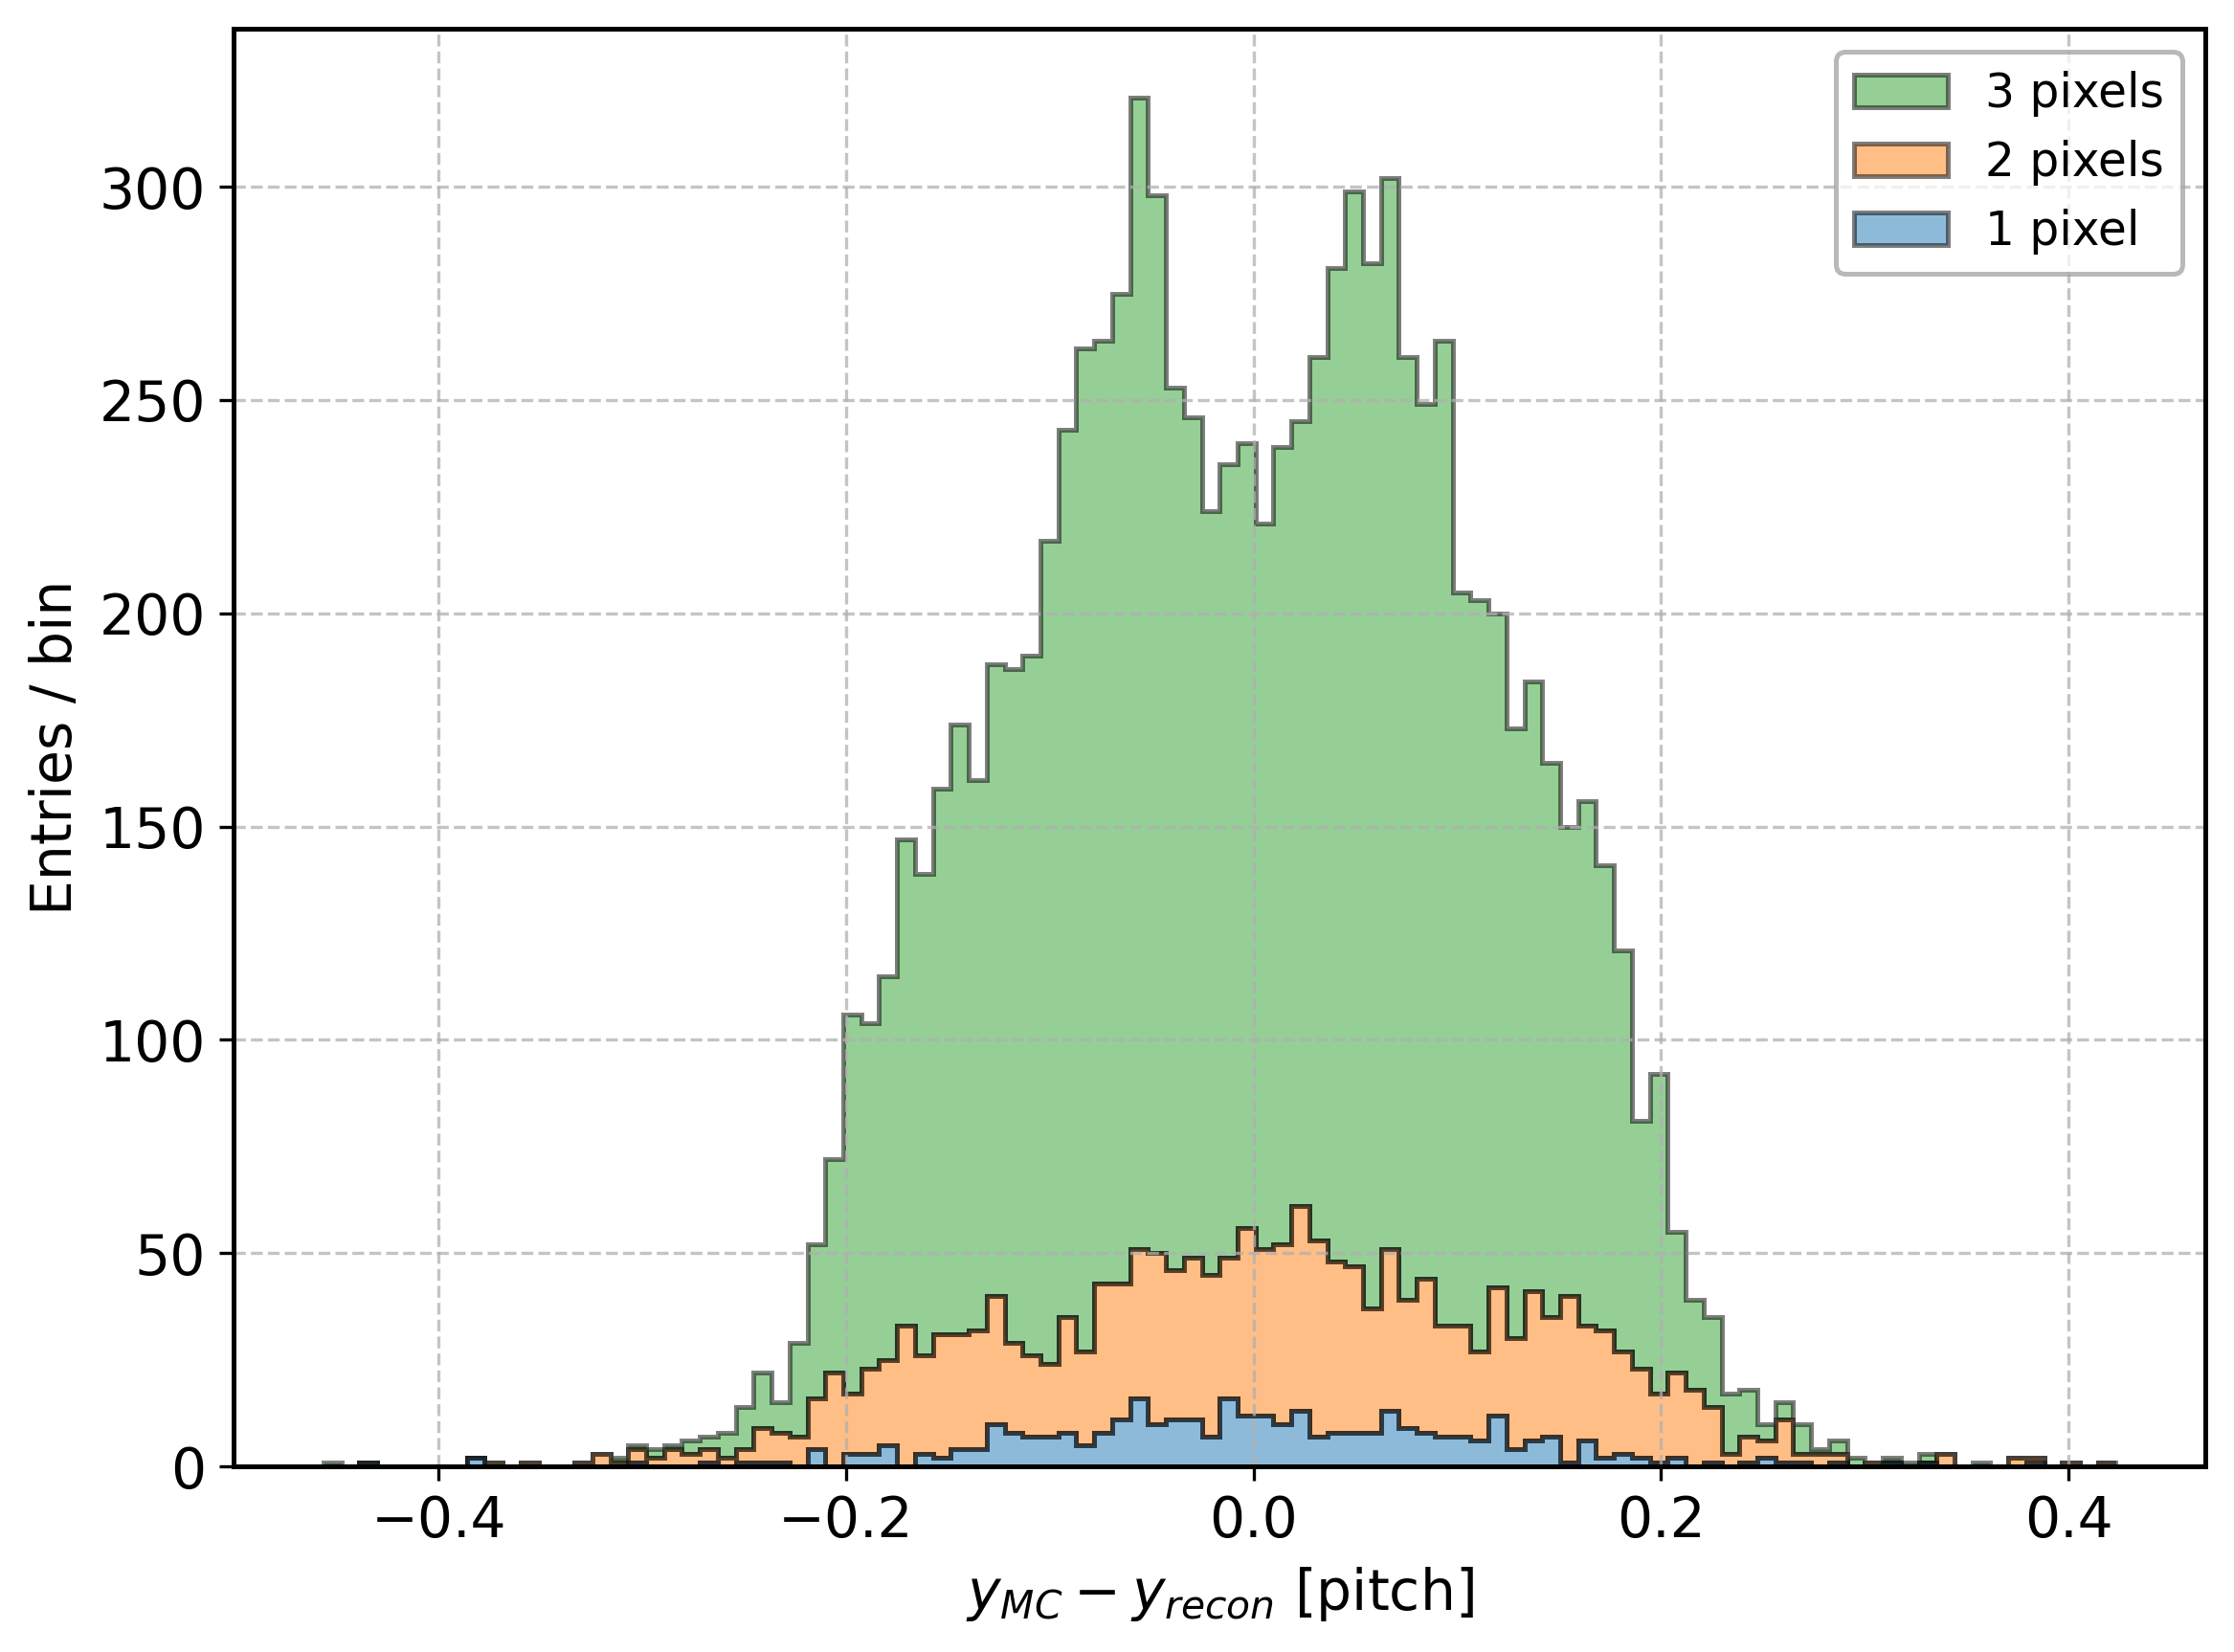
\includegraphics[width=0.49\linewidth]{figures/chapter4/position/barycenter_dy}
    \caption{Residuals distributions for the $x$ and $y$ directions obtained with the charge barycenter algorithm. The residuals are calculated as the difference between the reconstructed and the Monte Carlo truth $x$ and $y$ components. The events are separated by cluster size, with each color representing a specific cluster size. The histograms are stacked on each other. The simulation is made with a 8 keV monochromatic source, 20 ENC of noise and a silicon sensor 300 $\mu$m thick, with a $\langle \sigma \rangle / p = 15$\% .}
    \label{fig:barycenter_dx_dy}
\end{figure}

This method assumes that the charge in each pixel is spread uniformly across it or, equivalently, that it is concentrated in its center. This method does not consider how the charge diffuses inside the active sensor. If the charge would spread on a large number of pixels, this assumption would be valid and the charge barycenter would be a good estimator of the incident position. However, as said above, the detectors are designed to have a small $\langle \sigma \rangle / p$ ratio and the cluster size is small, thus the charge barycenter is not ideal.

It must be noted that for one-pixel events this is the only possible method that can be applied, as there is not enough information to reconstruct a position different from the pixel center. From this point on, it is assumed that every time a one-pixel event is analyzed, the incident position is reconstructed in the pixel center. While these events have the best energy resolution, as will be shown in the next section, they have the worst spatial resolution.

Fig. \ref{fig:barycenter_dx_dy} shows the residuals distributions for the $x$ and $y$ components between the reconstructed and the Monte Carlo truth positions. It is visible how the hexagonal geometry affects the reconstruction, in particular for two-pixels and three-pixels events. The overall distributions are not gaussians and are broad.

By calculating the distance between the truth and the reconstructed positions, the EEF can be calculated. 
Fig. \ref{fig:barycenter_eef} shows how the EEF of the barycenter algorithm varies as a function of the ratio between the diffusion widths of the charge cloud and the pixel pitch. It can be observed that a broader diffusion implies a better resolution. 
%Tab. \ref{tab:eef_barycenter} shows the distance at which EEF contains 50\% and 90\% of the events.

%\begin{table}[htbp]
%\centering
%\begin{tabular}{c cccc}
%$\langle \sigma \rangle / p$ [\%] & EEF@50\% [pitch] & EEF@90\% [pitch]\\
%\midrule
%12.2 & 0.19 & 0.27 \\
%13.7 & 0.17 & 0.24 \\
%15.2 & 0.15 & 0.22 \\
%16.8 & 0.13 & 0.20 \\
%18.3 & 0.11 & 0.18 \\
%\bottomrule
%\end{tabular}
%\caption{Pitch distances at which EEF contains 50\% and 90\% of the events with charge barycenter reconstruction, as a function of the ratio $\langle \sigma \rangle / p$. The values are extracted from Fig. \ref{fig:barycenter_eef}}
%\label{tab:eef_barycenter}
%\end{table}

This algorithm does not require any specific position-calibration models, as it neglects the physical details of charge diffusion. Consequently, it represents a fast, straightforward approach that provides a robust first estimate of the interaction position, relying exclusively on basic noise and gain-corrected pixel data.

\begin{figure}[h]
    \centering
    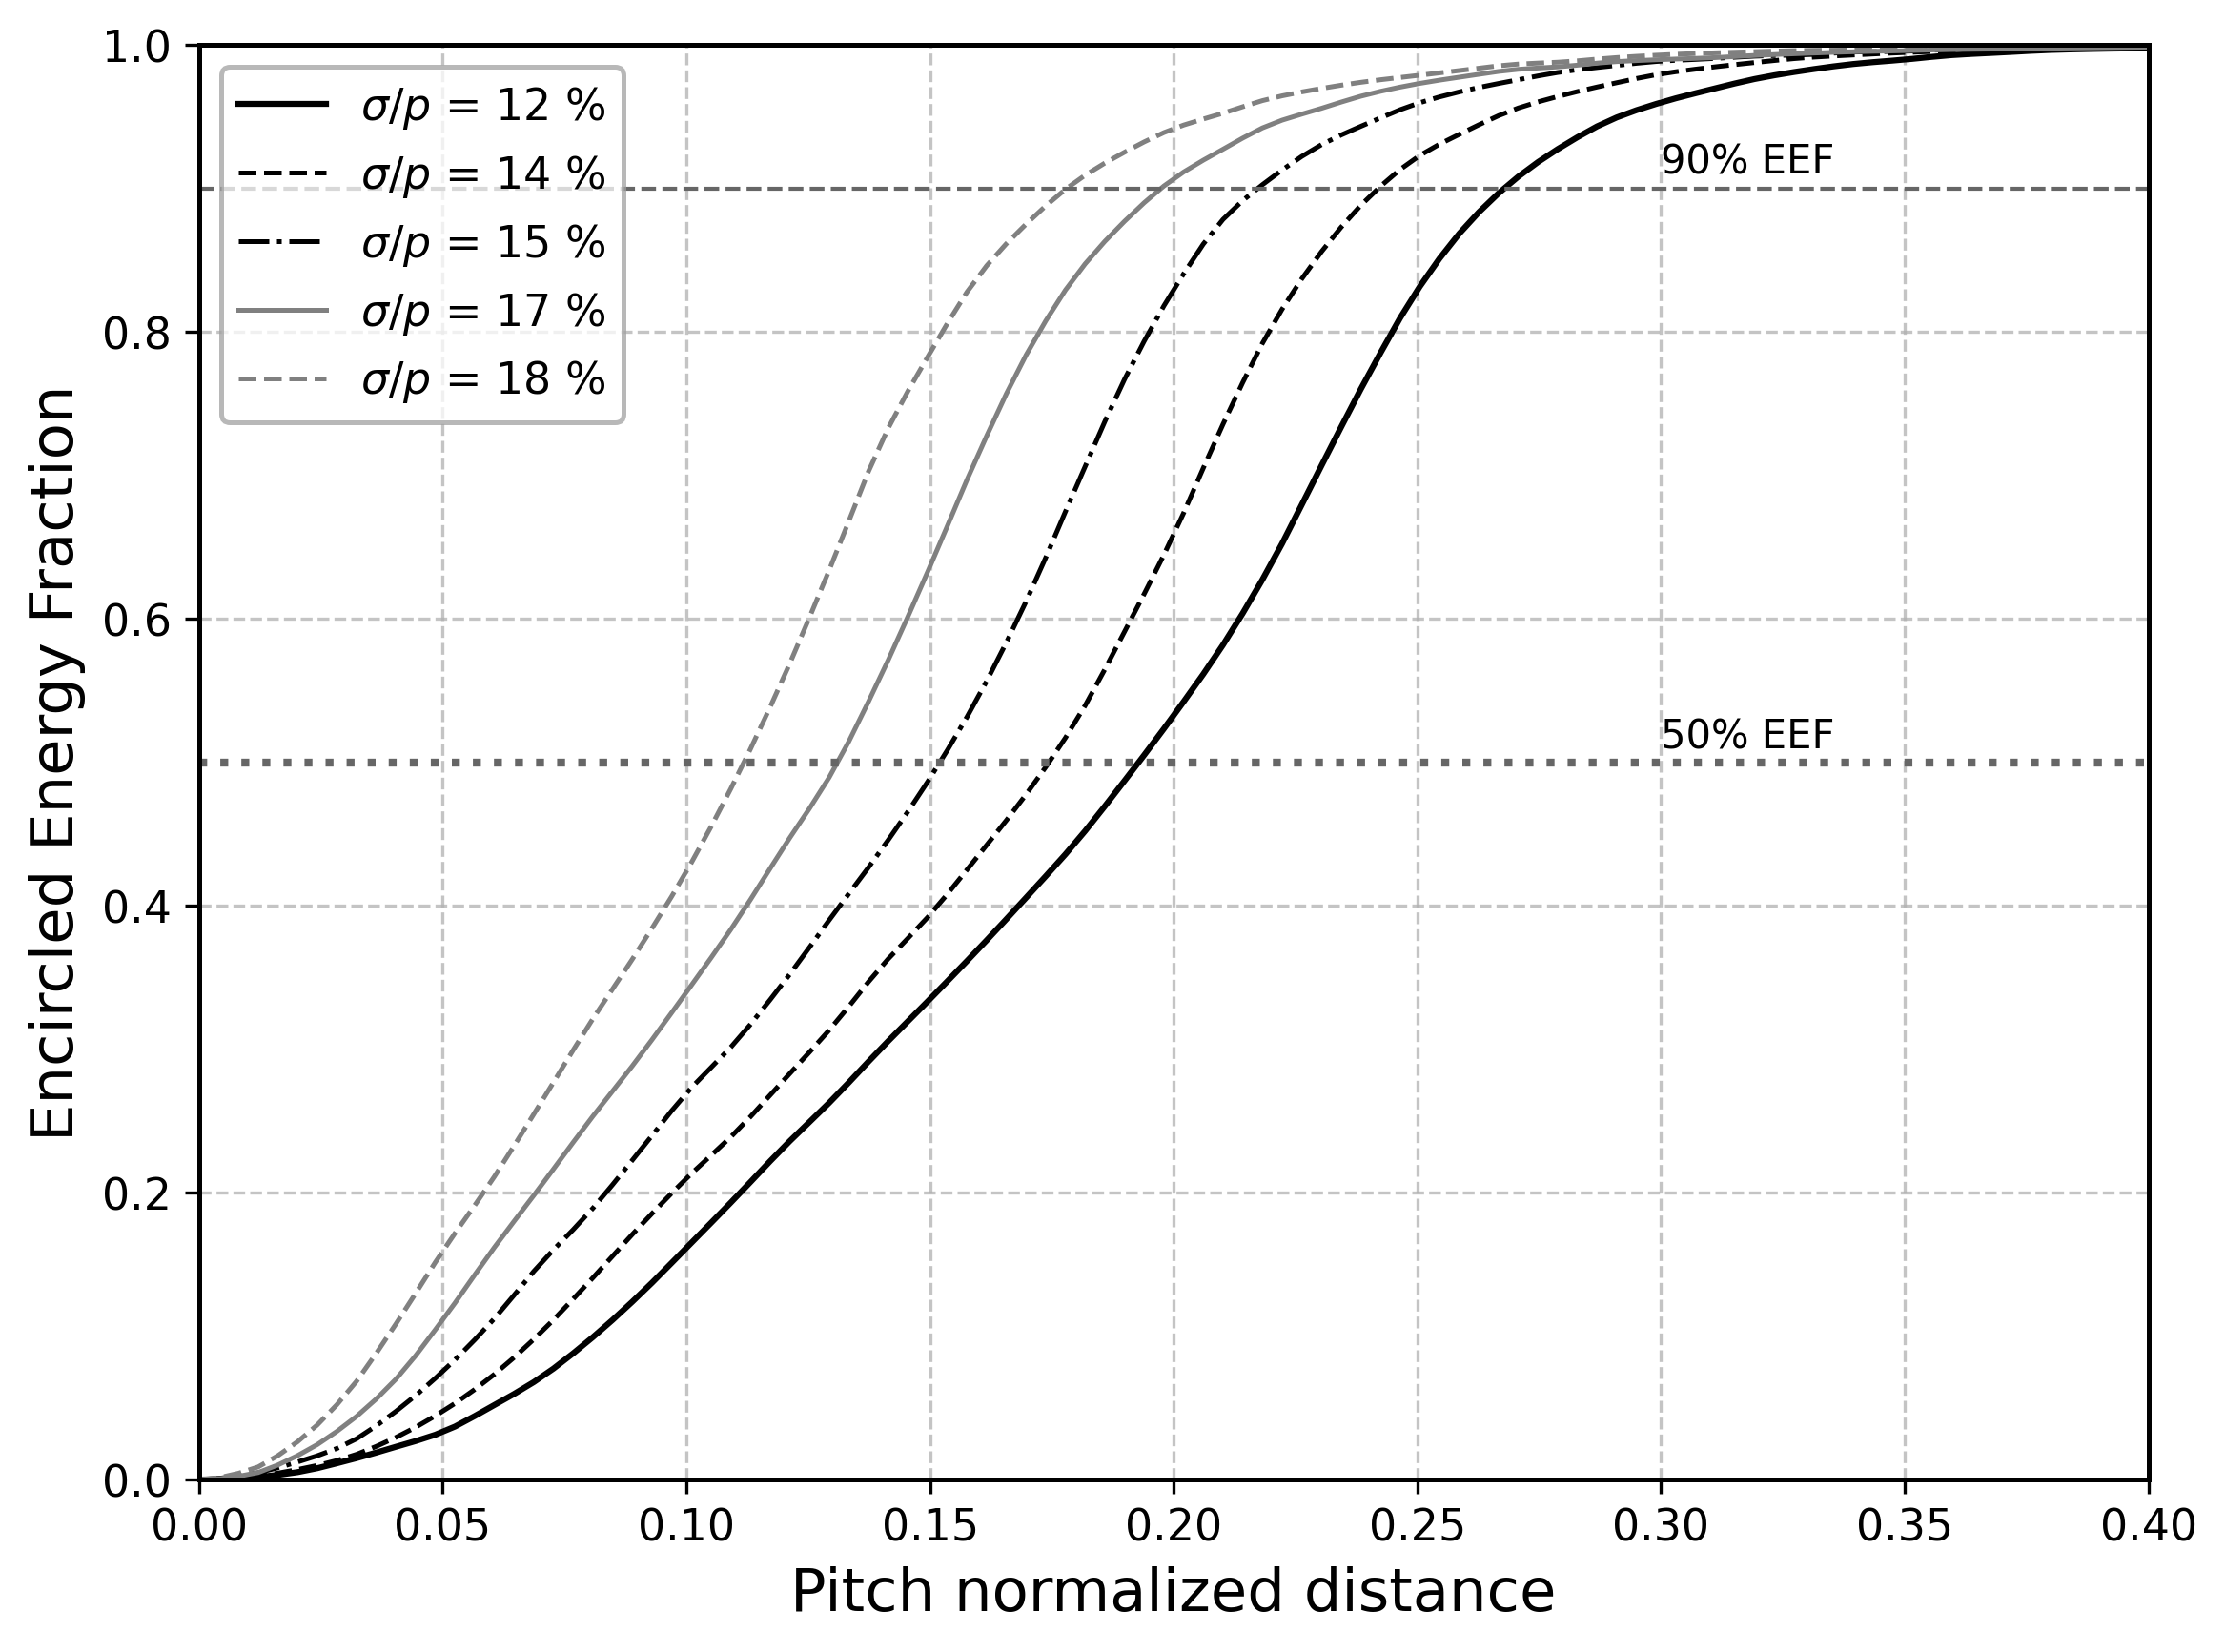
\includegraphics[width=0.7\linewidth]{figures/chapter4/position/barycenter_eef}
    \caption{EEF for different values of the ratio between the diffusion cloud widths and the pixel pitch as a function of the pitch normalized distance. The simulations are made with 20 ENC of noise and a silicon sensor 300 $\mu$m thick. To vary $\langle \sigma \rangle / p$ the diffusion coefficient is varied in the range 40--60 $\mu$m cm$^{-0.5}$.}
    \label{fig:barycenter_eef}
\end{figure}

\subsection{Likelihood estimator}
\label{subsec:mle}

\begin{figure}[!b]
    \centering
    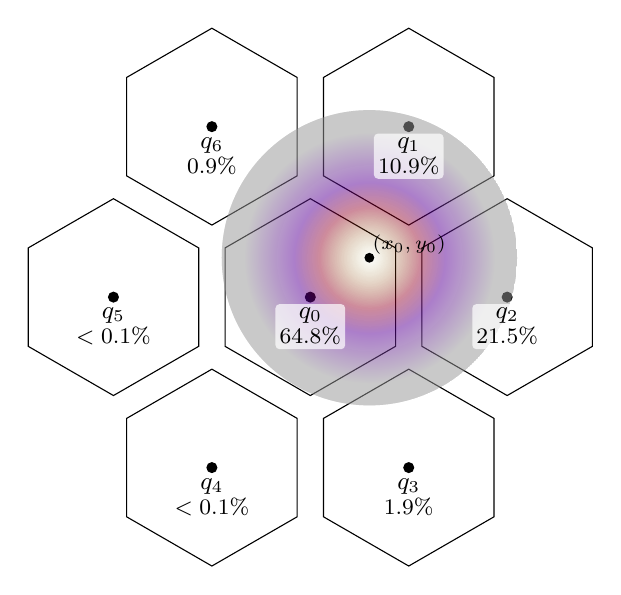
\begin{tikzpicture}[scale=2.5]

    \hexpix{\hexsize}
    \hexpix[xshift=1cm]{\hexsize}
    \hexpix[xshift=-1cm]{\hexsize}
    \hexpix[xshift=0.5cm, yshift=-0.866cm]{\hexsize}
    \hexpix[xshift=-0.5cm, yshift=-0.866cm]{\hexsize}
    \hexpix[xshift=0.5cm, yshift=+0.866cm]{\hexsize}
    \hexpix[xshift=-0.5cm, yshift=+0.866cm]{\hexsize}
    
    \begin{scope}
        \clip (0.3,0.2) circle (0.75cm);
        \fill[shading=paletteScienza, path fading=gaussianaPerfetta, opacity=0.3] (0.3,0.2) circle (0.75cm);
    \end{scope}
    
    \tikzset{
        labelStyle/.style={
            anchor=center, 
            font=\small, 
            text=black, 
            align=center,
            fill=white, 
            fill opacity=0.7, 
            text opacity=1, 
            inner sep=1.5pt, 
            rounded corners=1.5pt
        }
    }

    \node[labelStyle] at (0, -0.15) {$q_0$\\[-2pt]\footnotesize 64.8\%};
    \node[labelStyle] at (1, -0.15) {$q_2$\\[-2pt]\footnotesize 21.5\%};
    \node[labelStyle] at (0.5, 0.866-0.15) {$q_1$\\[-2pt]\footnotesize 10.9\%};
    \node[labelStyle] at (0.5, -0.866-0.15) {$q_3$\\[-2pt]\footnotesize 1.9\%};
    \node[labelStyle] at (-0.5, 0.866-0.15) {$q_6$\\[-2pt]\footnotesize 0.9\%};
    \node[labelStyle] at (-0.5, -0.866-0.15) {$q_4$\\[-2pt]\footnotesize $<0.1\%$};
    \node[labelStyle] at (-1, -0.15) {$q_5$\\[-2pt]\footnotesize $<0.1\%$};

    \fill[black] (0.3, 0.2) circle (0.025cm);
    \node[anchor=south west, font=\scriptsize, text=black, inner sep=1pt] 
        at (0.3, 0.2) {$(x_0, y_0)$};
        
    \end{tikzpicture}
    
    \caption{Example of charge diffusion from a photon with incident position $(x_0, y_0)$ and standard deviation of the bivariate Gaussian equal to 15\% of the pixel pitch. The charge cloud extends up to $5\sigma$, and the calculated charge fractions collected by each pixel ($q_0\text{--}q_6$) are explicitly indicated.}
    \label{fig:mle_model}
\end{figure}

The simple barycenter algorithm totally ignores how the charge diffuses inside the sensor, as it assumes that it uniformly spreads across the involved pixels. As mentioned in Chap. \ref{sec:semiconductors}, the charge diffusion inside the active sensor can be modeled with a bivariate Gaussian distribution centered on the incident position and with a standard deviation $\sigma$ that can be estimated using Eq. \ref{eq:z_average} and the working conditions of the sensor. By normalizing the total charge to 1, the integral of the bivariate distribution over each pixel $P_i$ represents the charge fraction $f_i$ that has been collected by it

\begin{equation}
f_i (x_0, y_0) = \int_{P_i} \frac{1}{2\pi \sigma^2} \exp \left[ - \frac{(x - x_0)^2 + (y - y_0)^2}{2\sigma^2} \right] \,dx\,dy.
\label{eq:mle_charge_fraction}
\end{equation}

The total charge of the event is defined as $Q = \sum_{i=0}^6 q_i$, where $q_i$ is the charge collected by the $i$-th pixel. Assuming that electronic noise is negligible and that charge fluctuations are purely statistical, the joint distribution of charges across the cluster follows a multinomial distribution. From this distribution, the likelihood of the photon incident position $(x, y)$ given the observed charges is defined as:

\begin{equation}
\mathcal{L}(x, y) = \frac{Q!}{\prod_i q_i!} \prod_i f_i(x,y) ^{q_i}.
\label{eq:mle_multinomial}
\end{equation}

If electronic noise is present, the pure multinomial model no longer holds, especially in high-noise conditions, because the observed charge fluctuations become dominated by signal-independent electronic noise rather than charge-partition statistics. 

An example to illustrate this situation is the case of a $8\text{ keV}$ photon absorbed in a silicon sensor, which generates approximately $Q \approx 2200\text{ e}^-$ electron-hole pairs. If the central pixel collects an expected fraction $f_0 = 40\%$ of the total charge, the variance associated with the binomial charge-sharing partition among the pixels is

\begin{equation}
\sigma_{\text{s}}^2 = Q f_0 (1 - f_0) \approx 528.
\end{equation}

For the design goal electronics noise of $\sigma_n = 20\text{ ENC}$, the electronic noise variance is $\sigma_n^2 = 400$. Even for the pixel collecting the largest charge fraction, the statistical partition variance $\sigma_{\text{s}}^2$ and the electronic noise variance $\sigma_n^2$ are of comparable magnitude. For neighboring pixels collecting smaller fractions ($f_i \ll 1$), the partition variance scales as $\sigma_{\text{s}}^2 \approx Q f_i$ and becomes completely overwhelmed by the electronic noise.

To correct this model and adapt it to the presence of electronic noise it is necessary to consider how the noise affects the observations. As seen in Sec. \ref{sec:noise_calibration}, the noise is distributed according to a Gaussian distribution. As a consequence, each pixel charge distribution can be modeled with a Gaussian distribution for the following reasons:

\begin{itemize}[label=-]
\item if a pixel collects many charges, its probability distribution converges to a Gaussian distribution. When the noise is added, the resulting variable is still distributed according to a Gaussian distribution with variance $\sigma^2 = \sigma^2_s + \sigma^2_n$;

\item if a pixel collects a small fraction of charge, its charge distribution follows a binomial distribution with a small probability parameter $f_i$. This distribution is highly asymmetrical, peaked near zero and with a very low variance $\sigma^2_s$, negligible with respect to the electronic noise variance $\sigma^2_n$. This means that when summing the two variables, the noise dominates the signal charge, with the resulting distribution being a Gaussian distribution, whose variance can still be modeled as the sum of the two independent components $\sigma^2 = \sigma^2_s + \sigma^2_n$.
\end{itemize}

Therefore, the charge probability density function of a single pixel is

\begin{equation}
p(q_i; \mu = f_i Q , \sigma^2) = \frac{1}{\sqrt{2\pi}\sigma} \exp \left[- \frac{(q_i - f_i Q)^2}{2\sigma^2} \right],
\label{eq:pdf_mle}
\end{equation}

where $\sigma$ is the standard deviation obtained from the squared sum of the two fluctuation components and $Q$ is the true total charge generated by the photon interaction. It is important to note that, unlike the electronic noise-free scenario, the true charge $Q$ is now an unknown parameter, because the independent electronic noise added to each pixel causes the sum of the measured charges $\sum_i q_i$ to deviate from the true value $Q$.

Eq. \ref{eq:pdf_mle} lacks an important characteristic which is included in Eq. \ref{eq:mle_multinomial}, which is the correlation between the pixels. Indeed, this probability density function does not take into account the fact that if the incident position varies a bit, some pixels lose some of the charge, while others increase it, thus it cannot be assumed that the pixels are independent. To take the pixel correlation into account, a model that takes into account all the pixels at once has to be considered.

To this end, the probability density function is a generic multivariate Gaussian distribution, described by

\begin{equation}
p(\vec{q}; x, y, Q) = \frac{1}{(2 \pi)^{7/2} |V|^{1/2}} \exp{\left[ -\frac{1}{2}(\vec{q} - \vec{f}Q)^{T} V^{-1} (\vec{q} - \vec{f}Q) \right]},
\label{eq:multivariate_gauss}
\end{equation}
where $\vec{q}$ is the seven-dimensional vector with the observed pixels charge, $\vec{f}$ is the vector with the charge fraction values, and $V$ is the covariance matrix, for which the diagonal elements are the squared sums of the multinomial variances and noise fluctuations and off-diagonal elements are the covariances obtained from the multinomial model, which describe the charge sharing mechanism of the cloud

\begin{equation}
V_{ii} = \sigma^2_{s,i} + \sigma^2_{n,i}, \quad \quad V_{ij} = - Q f_i f_j \quad \textrm{for } i \neq j.
\label{eq:cov_matrix}
\end{equation}

For the off-diagonal elements of the covariance matrix the assumption that electronic noise is uncorrelated is made.

In Eqns. \ref{eq:multivariate_gauss} and \ref{eq:cov_matrix}, the dependance from the incident position is hidden inside $\vec{f}$, so both the mean vector and the covariance matrix depend on the unknown parameters $(x, y)$. At this point, the negative log-likelihood can be computed from Eq. \ref{eq:multivariate_gauss} as

\begin{equation}
\operatorname{NLL}(x, y, Q) = -\ln \mathcal{L} = \frac{1}{2}(\vec{q} - \vec{f}Q)^{T} V^{-1} (\vec{q} - \vec{f}Q) +  \frac{1}{2} \ln |V| + \textrm{const.}
\label{eq:nll_multivariate}
\end{equation}

\begin{figure}[!b]
    \centering
    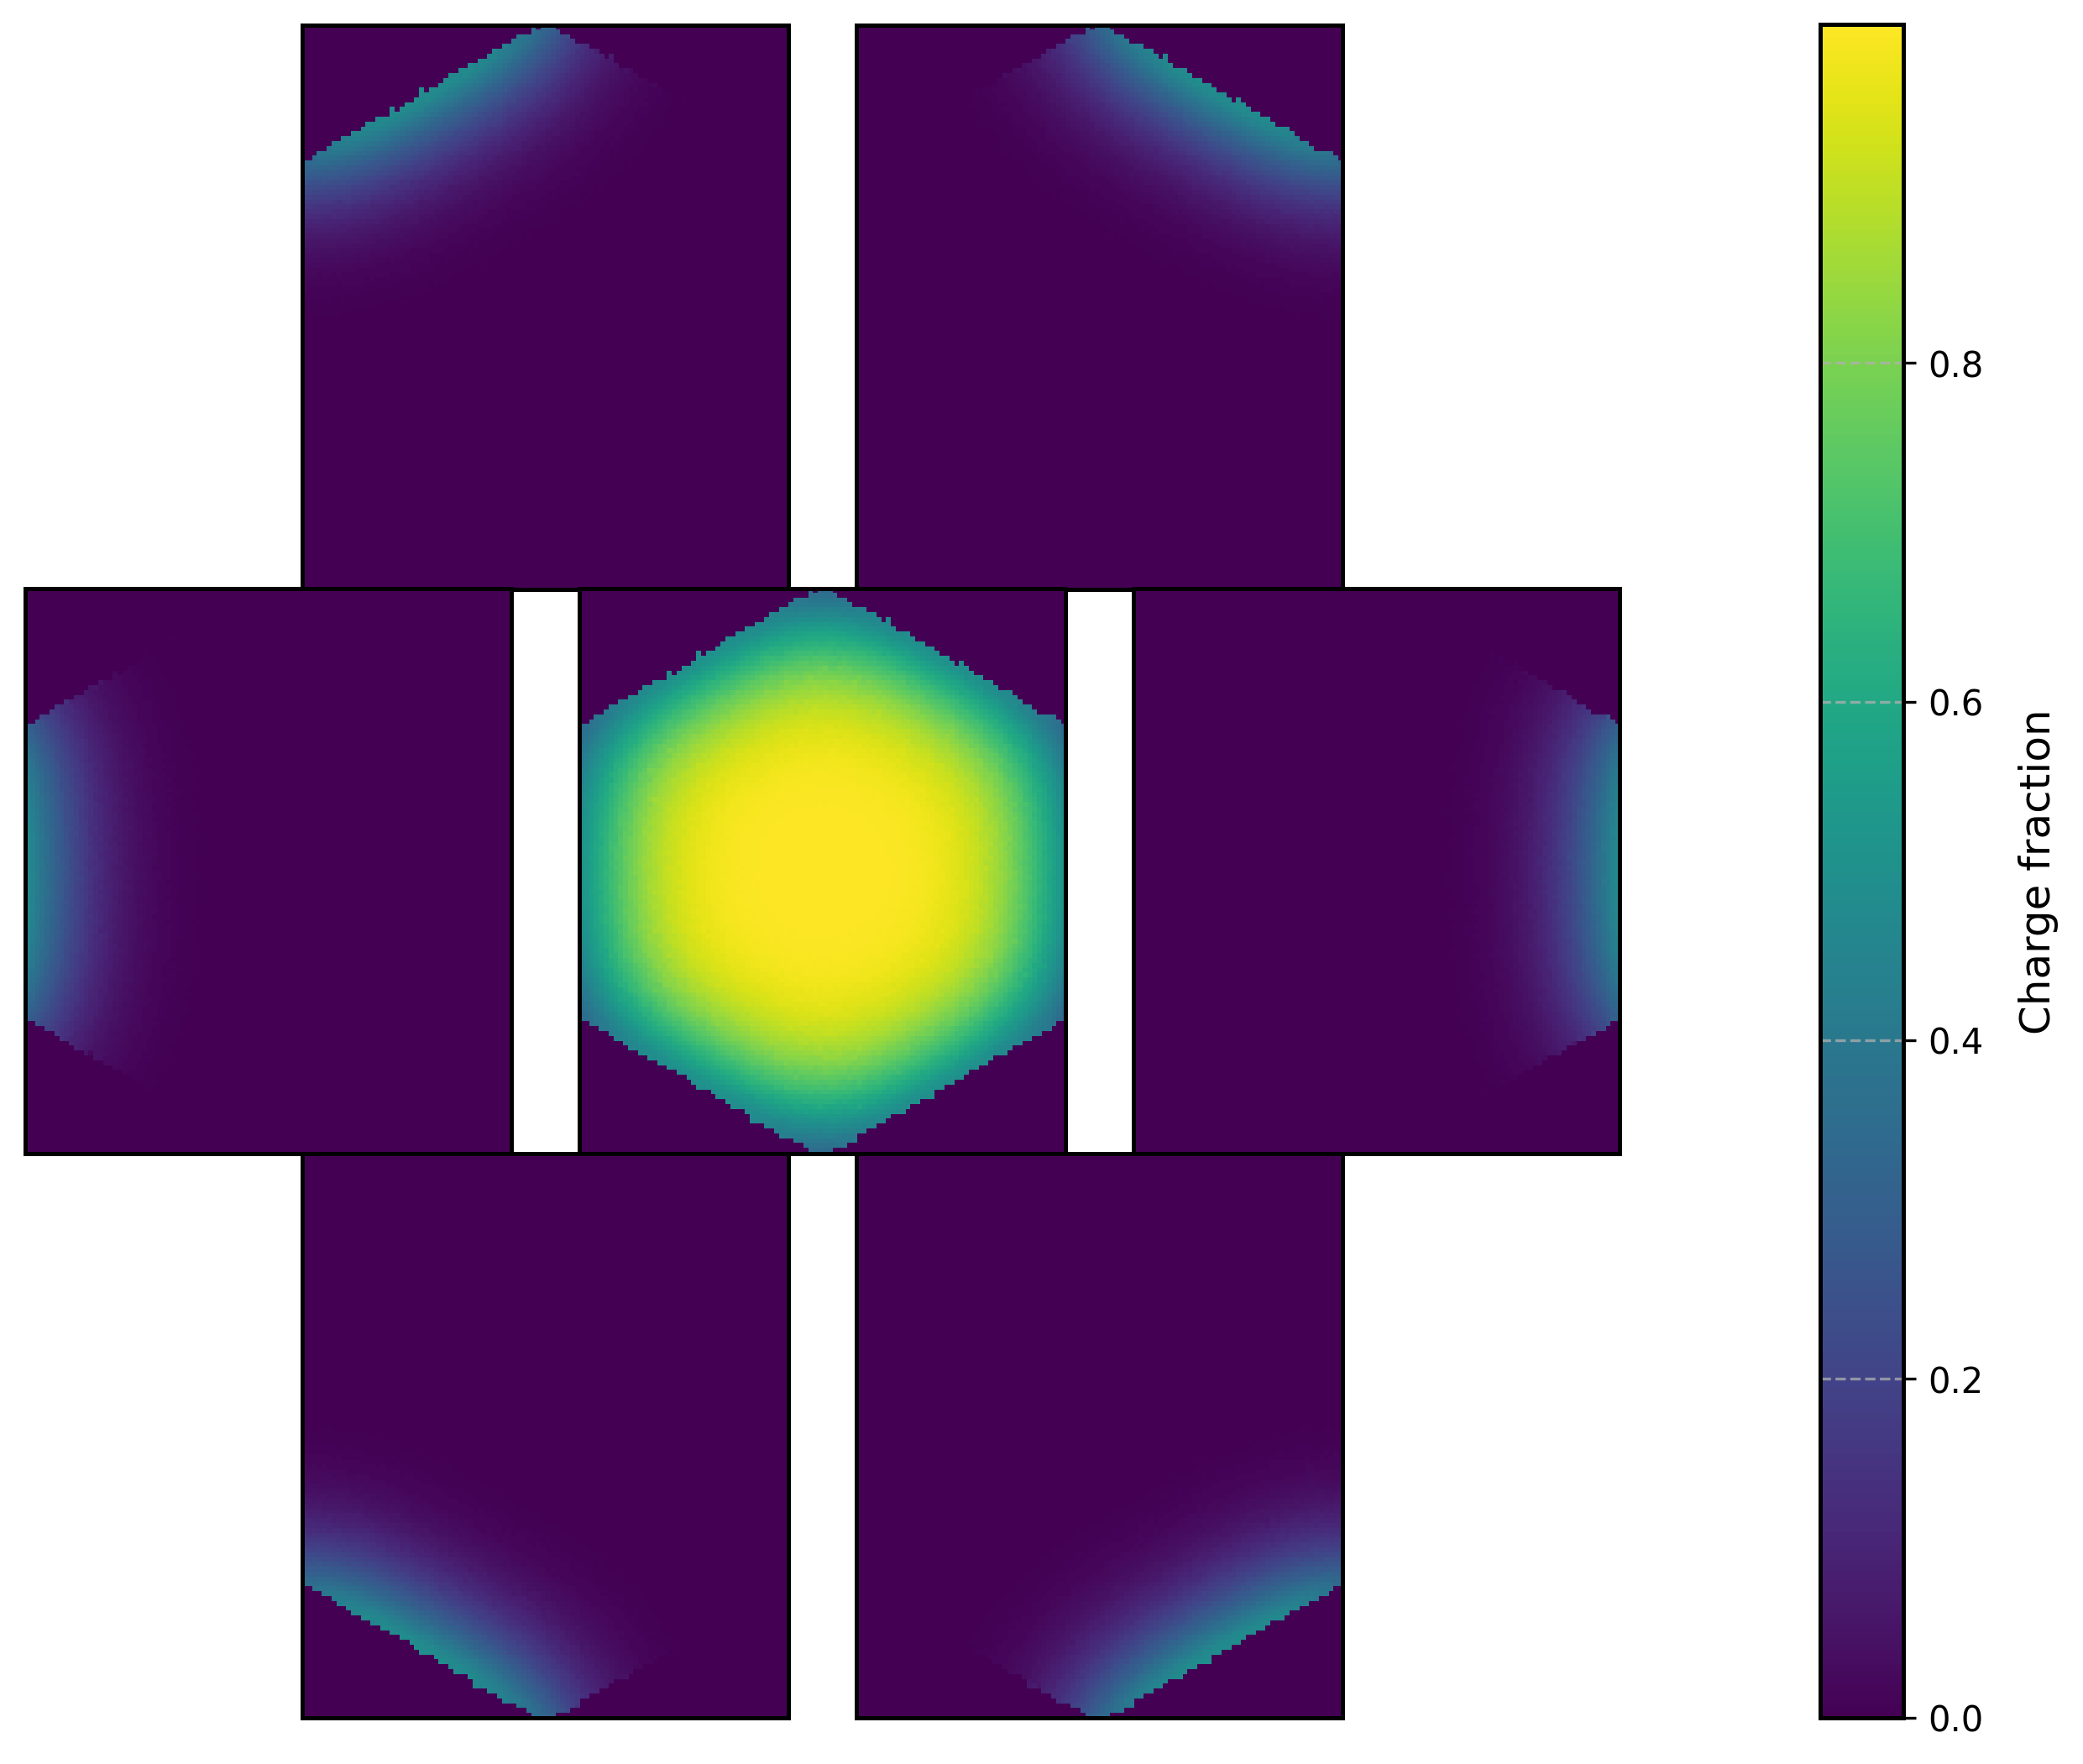
\includegraphics[width=0.48\linewidth]{figures/chapter4/position/calibration_matrices}
    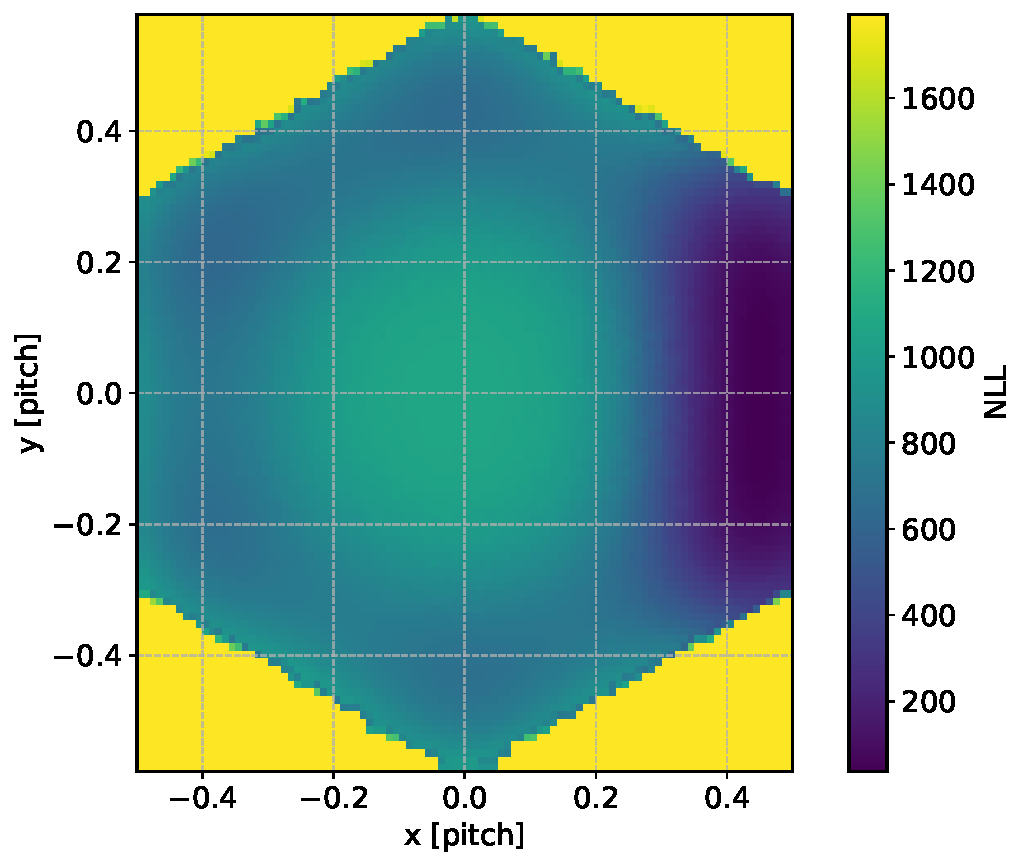
\includegraphics[width=0.48\linewidth]{figures/chapter4/position/nll}
    \caption{Left panel: the seven charge fraction calibration matrices evaluated as a function of the impact position on the central pixel, simulated for a 6 keV monochromatic source with $\langle \sigma \rangle / p \approx 13\%$. The grid is composed of $100 \times 116$ bins. Right panel: two-dimensional map of the $\operatorname{NLL}$ evaluated across the central pixel for a fixed charge $Q$, where the minimum identifies the best-fit reconstructed position $(\hat{x}, \hat{y})$. In the actual fit, $Q$ is free and the minimization is performed in the 3D space $(x, y, Q)$.}
    \label{fig:mle_calibration_and_nll}
\end{figure}

This equation can now be minimized with respect to the unknown parameters $(x, y, Q)$ to find the best-fit incident position and total charge of the event. The minimization is performed with \textit{iminuit} \cite{iminuit}. 

In order to be correctly used, this position reconstruction method requires a prior calibration of the diffusion model. Indeed, the charge fractions depend on the charge cloud diffusion width. The charge fractions $f_i$ could be numerically calculated with Eq. \ref{eq:mle_charge_fraction}, but the hexagonal geometry of the pixels makes the calculation complex. For this reason, the charge-sharing model is evaluated through Monte Carlo simulations and tabulated for a certain value of the $\langle \sigma \rangle / p$ ratio, which is specific to a combination of sensor thickness, pixel pitch, diffusion coefficient and photon energy.

The charge-sharing model calibration is performed using a simulation without noise. A large number of monochromatic events are simulated, then the cluster central pixel is divided into a grid of square bins. For each position bin the average of the charge fraction collected by each of the seven pixels is calculated. The result of the calibration is a set of seven matrices, one for each pixel. Up to a reflection, the matrices of the outer pixels are identical, but for numerical simplicity they are saved and used independently. An example of the set of seven matrices is shown in Fig. \ref{fig:mle_calibration_and_nll}.

During the fit, the minimizer evaluates the $\operatorname{NLL}$ for various values of $(x, y, Q)$. An example of the $\operatorname{NLL}$ evaluated across the pixel for a fixed charge $Q$ is shown in Fig. \ref{fig:mle_calibration_and_nll}. Further details on how the evaluation and minimization of the $\operatorname{NLL}$ are performed are provided in Appendix \ref{appendix:mle}.

\begin{figure}[!b]
    \centering
    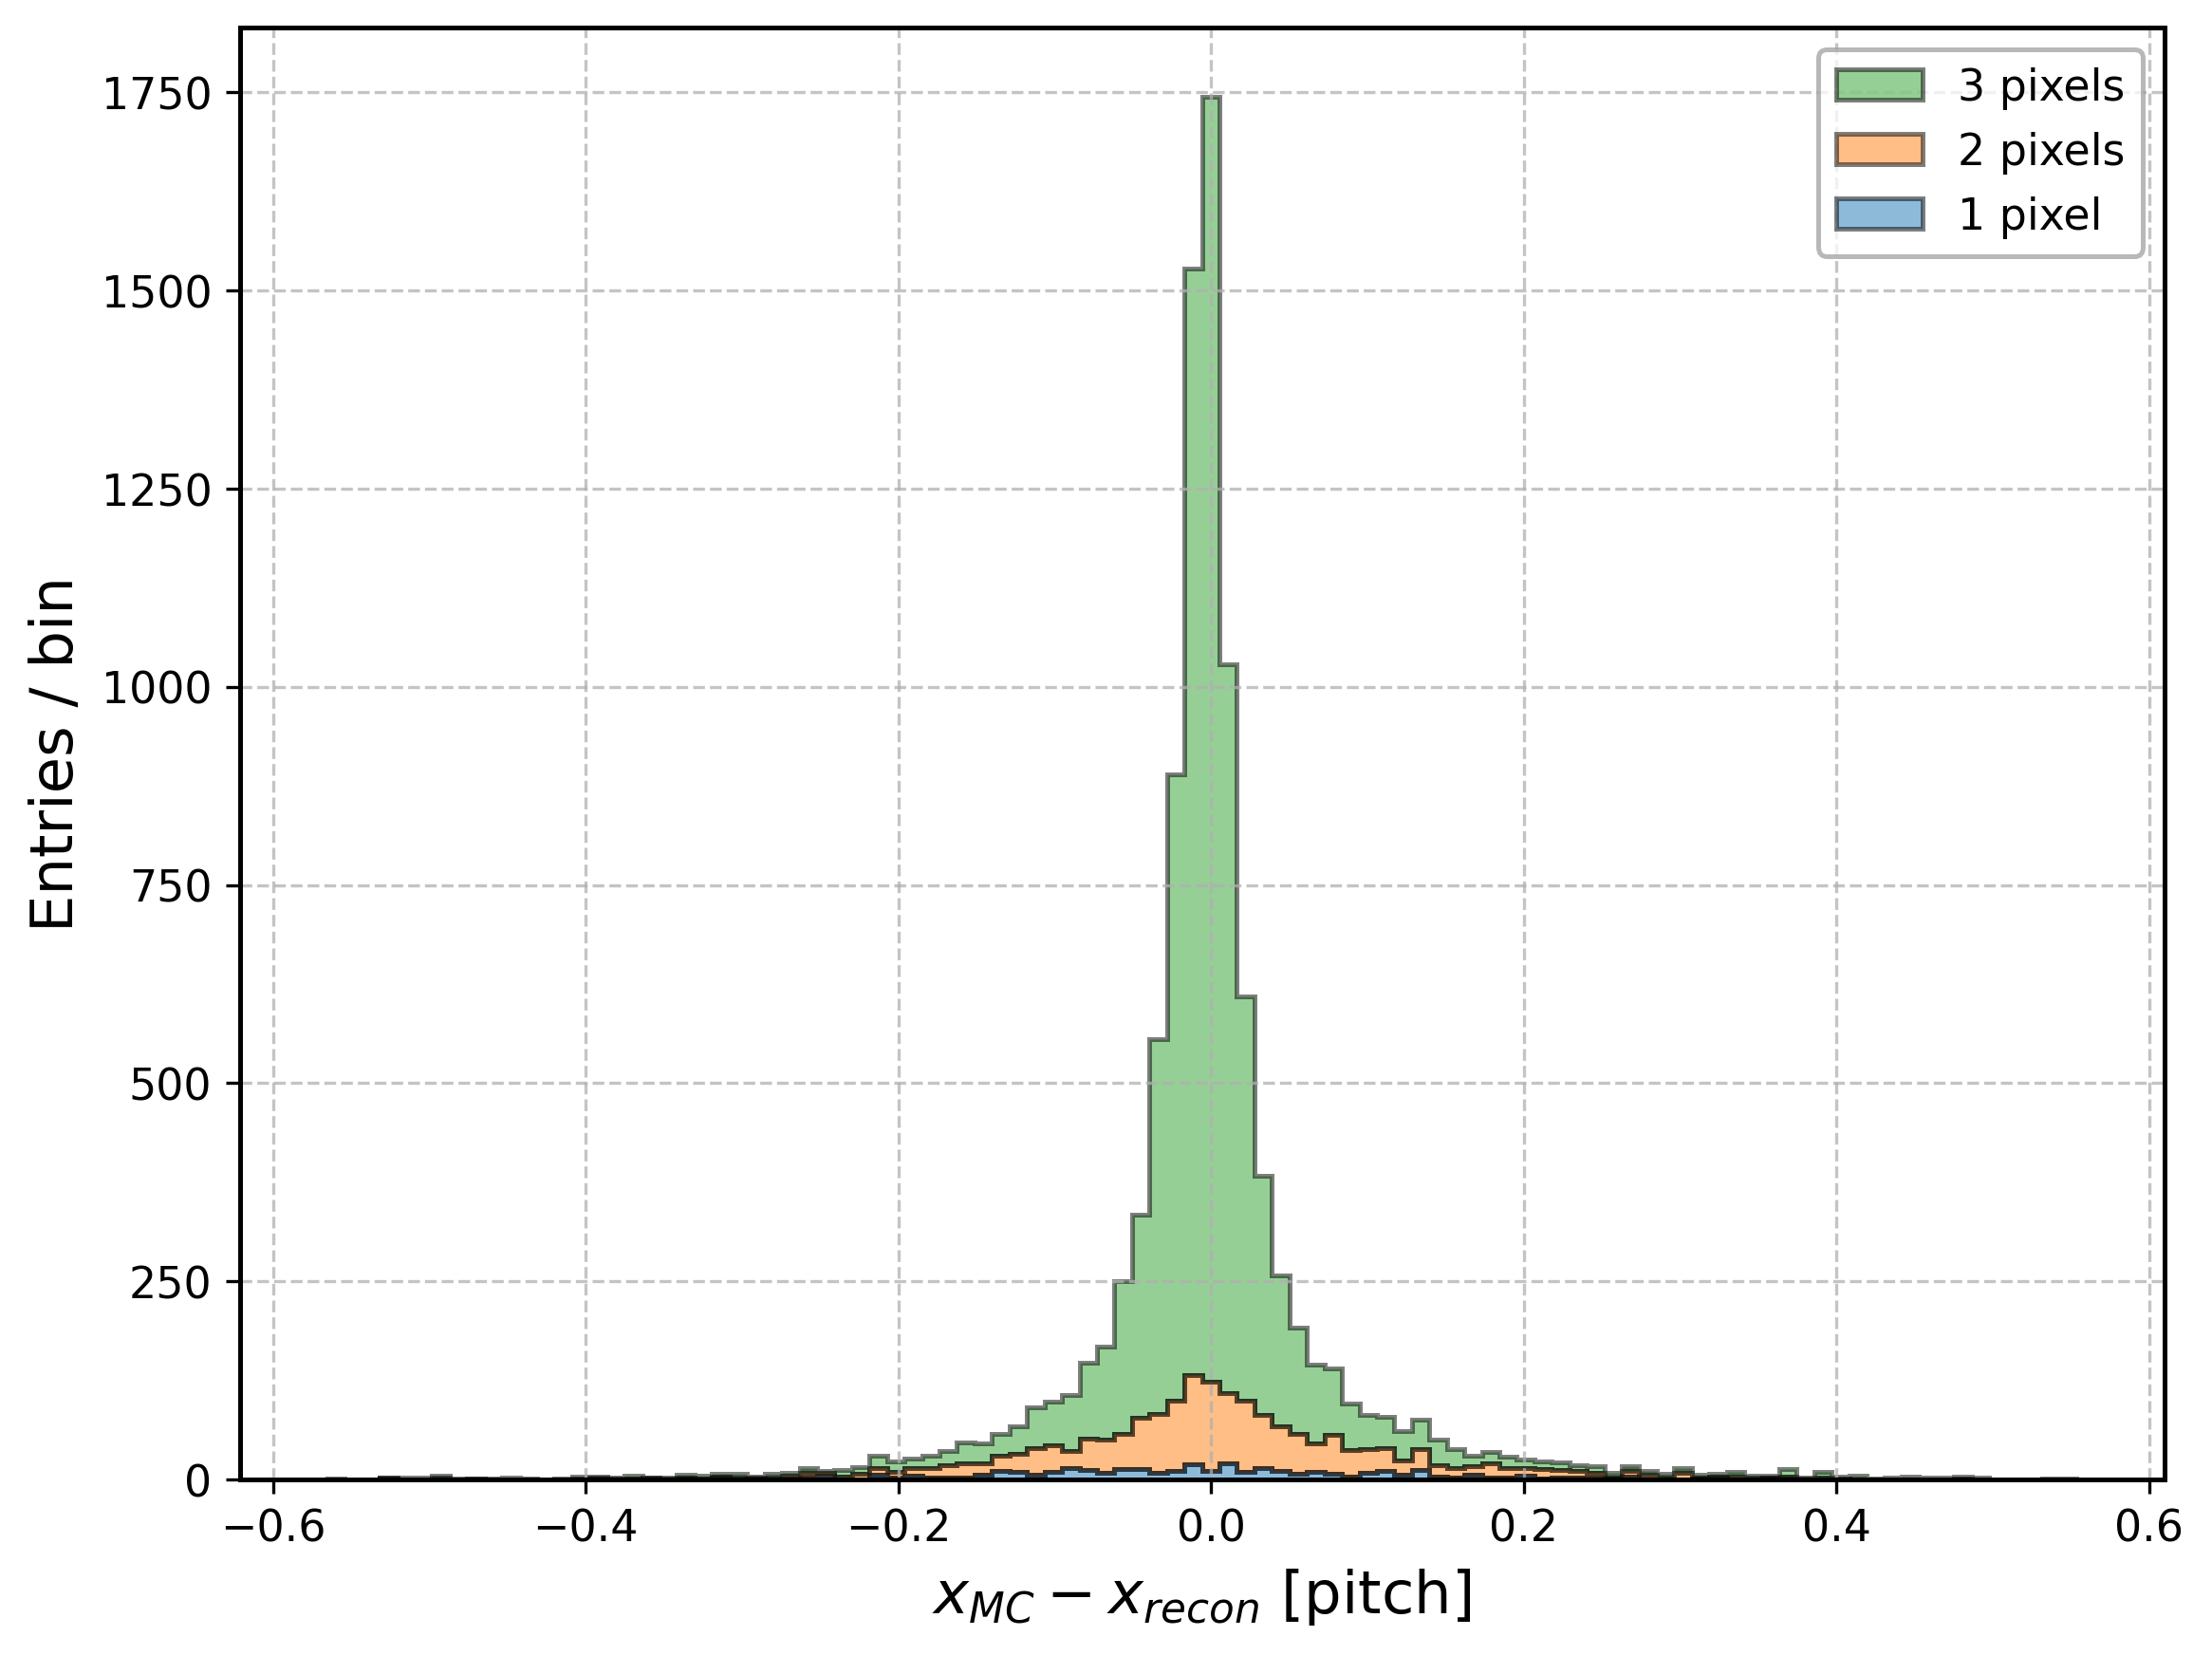
\includegraphics[width=0.49\linewidth]{figures/chapter4/position/mle_dx}
    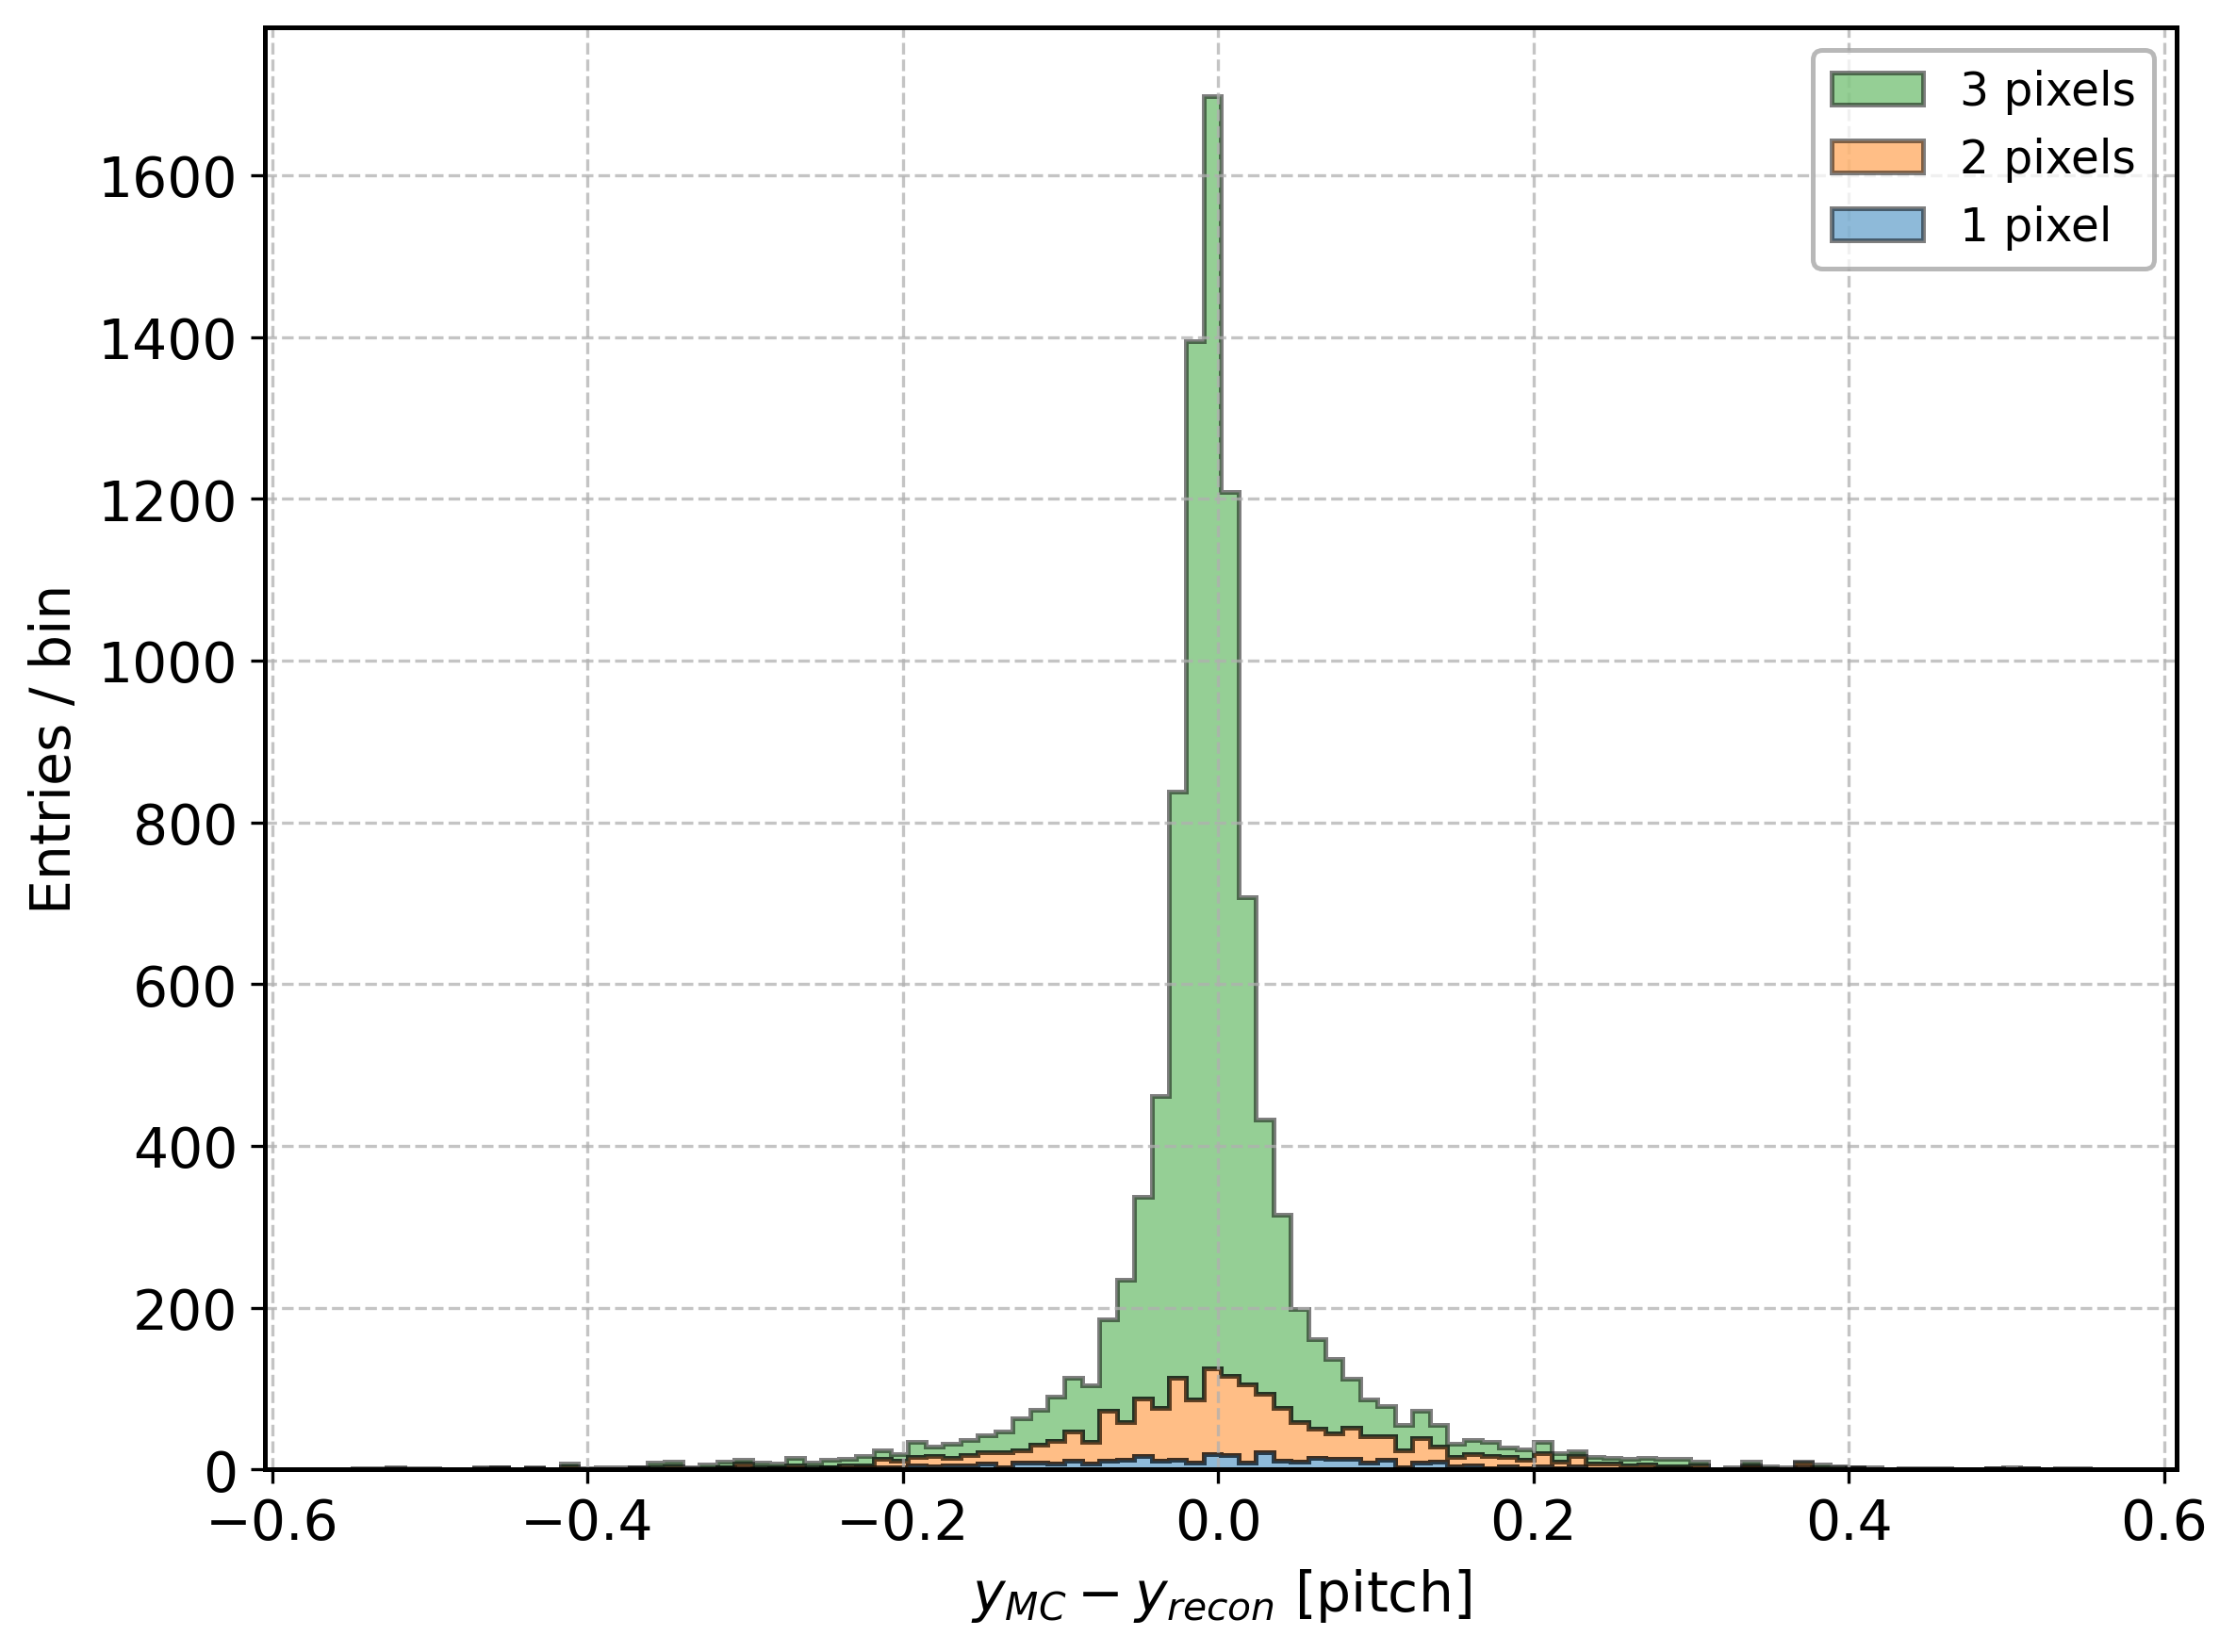
\includegraphics[width=0.49\linewidth]{figures/chapter4/position/mle_dy}
    \caption{Residuals distributions of the maximum likelihood reconstruction algorithm for the $x$ and $y$ directions, calculated as the difference between the reconstructed and the Monte Carlo truth $x$ and $y$ components. The events are separated by cluster size, with each color representing a specific cluster size. The histograms are stacked on each other. Cluster sizes are obtained from the reconstruction described in Sec. \ref{subsec:barycenter}. The simulation is made with a 8 keV monochromatic source, 20 ENC of noise and ratio between the diffused charge cloud sigma and the pitch of 15\%.}
    \label{fig:mle_dx_dy}
\end{figure}

Contrary to charge barycenter, this algorithm does not implement any type of suppression. Indeed, while charge barycenter applies a zero-suppression threshold and a position-suppression to suppress pixels that have high probability of having only noise signal, this algorithm weights each pixel by considering their charge and the calibrated diffusion model. As a consequence, defining the cluster size becomes ambiguous. For plotting purposes and to compare different algorithms, the cluster size used in Fig. \ref{fig:mle_dx_dy} to separate events is the cluster size that is obtained with the charge barycenter algorithm. Fig. \ref{fig:mle_dx_dy} shows the residuals distributions for the $x$ and $y$ position components. With this algorithm the residuals distributions are regular and unimodal. Moreover, the width of the distribution is much smaller than the previous algorithm. 

The only problem arises in the tails of the distributions, that show some residuals up to $\pm 0.6$ times the pixel pitch. This behaviour is well visible in Fig. \ref{fig:mle_eef}, where it is possible to see that the EEF has very long tails, particularly for small diffusion widths. This algorithm is generally better than the charge barycentering, indeed the EEF@50\% is always about three times smaller, but due to the long tails the EEF@90\% can be worse in some cases. 
%Tab. \ref{tab:eef_mle} shows exactly this feature because while the EEF@50\% is about three times smaller than the charge barycenter, the EEF@90\% can be worse in particular cases. 

Furthermore, the same dependence on the diffusion width as the charge barycenter can be observed, with broader diffusions that have a better spatial resolution. It must be noted that for the position reconstruction a set of calibration matrices has been produced for each diffusion width.

\begin{figure}[h]
    \centering
    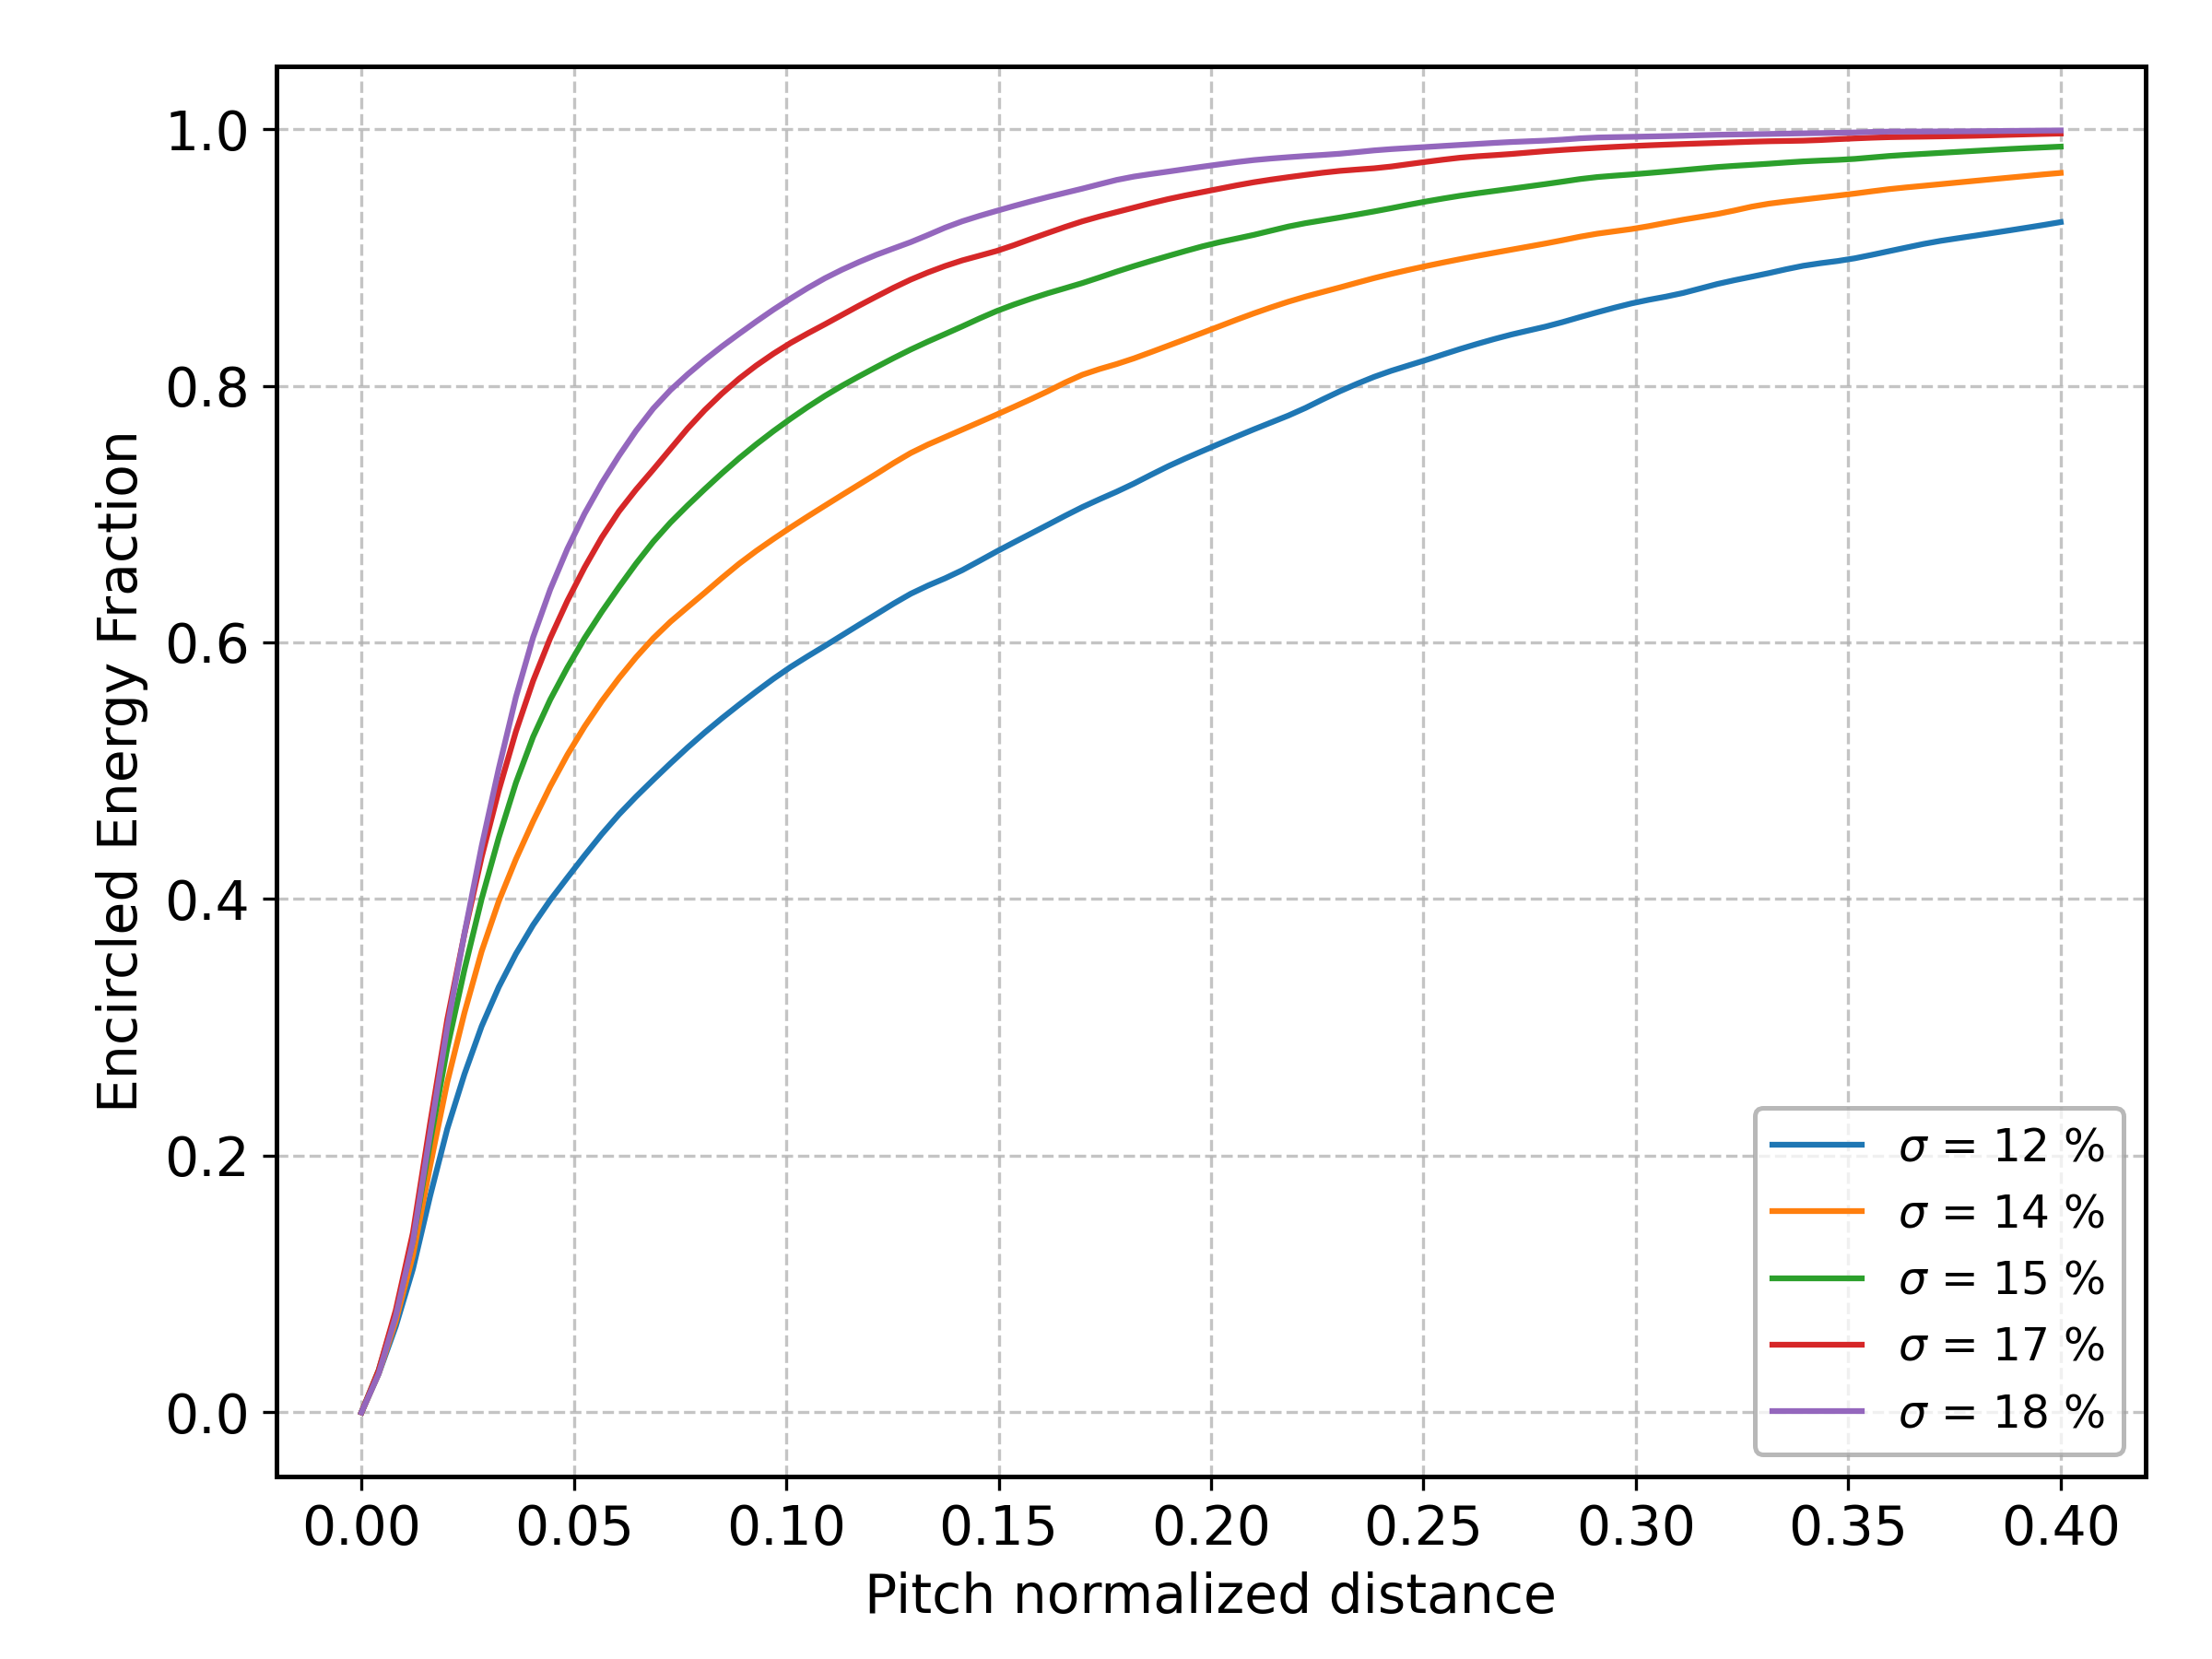
\includegraphics[width=0.7\linewidth]{figures/chapter4/position/mle_eef}
    \caption{Encircled energy fraction of the maximum likelihood estimator reconstruction for different values of the ratio between the diffused charge cloud and the pixel pitch as a function of the pitch normalized distance. The simulation is made with 20 ENC of noise.}
    \label{fig:mle_eef}
\end{figure}

%\begin{table}[htbp]
%\centering
%\begin{tabular}{c cccc}
%$\langle \sigma \rangle / p$ & EEF@50\% [pitch] & EEF@90\% [pitch]\\
%\midrule
%12.2 & 0.07 & 0.35 \\
%13.7 & 0.05 & 0.26 \\
%15.2 & 0.04 & 0.19 \\
%16.8 & 0.03 & 0.14 \\
%18.3 & 0.03 & 0.12 \\
%\bottomrule
%\end{tabular}
%\caption{Pitch distances at which EEF contains 50\% and 90\% of the events with maximum likelihood estimator reconstruction, as a function of the ratio $\langle \sigma \rangle / p$. The values are extracted from Fig. \ref{fig:mle_eef}}
%\label{tab:eef_mle}
%\end{table}


\subsection{$\eta$ algorithm}
\label{subsec:eta}
In the context of silicon microstrip detectors, a common and widely used algorithm to reconstruct the incident position of radiation is the so-called $\eta$ algorithm \cite{belau1983, turchetta1993}. This algorithm, in the case when only two strips have collected signal, is based on the definition of the $\eta$ variable

\begin{equation}
\eta = \frac{q_R}{q_L + q_R},
\label{eq:def_eta}
\end{equation}
that for a microstrip detector is the ratio between the charge $q_R$ collected by the right strip and the total charge collected by the two strips (right and left) involved in the event. By characterizing the distribution of this variable and studying the relation with the incident position, it is possible to obtain a non-linear algorithm, that contrary to the charge barycenter takes into account how the charge diffuses, like the maximum likelihood estimator algorithm.

Assuming that the events are uniformly distributed between the two strips, the typical distribution of $\eta$ is a U-shaped curve, peaked near $\eta = 0$ and $\eta = 1$ and symmetrical with respect to $\eta = 0.5$. The cumulative distribution of $\eta$ gives the relation between the distance from the left strip  of the impact point of the radiation and the observed value of $\eta$. The two distributions are shown in Fig. \ref{fig:belau_eta}.

\begin{figure}
    \centering
    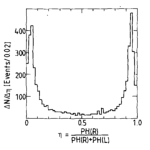
\includegraphics[width=0.45\linewidth]{figures/chapter4/position/belau_eta}
    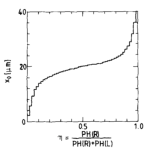
\includegraphics[width=0.45\linewidth]{figures/chapter4/position/belau_cumulative}
    \caption{In the left panel, experimental distribution of the $\eta$ variable calculated for a silicon microstrip detector. In the rigth panel, the cumulative distribution calculated from the latter, which gives the calibration function to reconstruct the event incident position. Images taken from \cite{belau1983}.}
    \label{fig:belau_eta}
\end{figure}

This methodology can also be generalized to the case of hexagonal pixel detectors, but there are some things that need to be modified. The main difference is the two-dimensional nature of position reconstruction on hexagonal pixels. For this reason, the discussion has to be separated depending on the cluster size. The second difference is that, contrary to microstrips, projecting the events belonging to a specific cluster size onto the chosen reconstruction axis does not yield a uniform one-dimensional distribution. Even under a perfectly uniform 2D illumination of the sensor, this projection is inherently non-uniform due to the hexagonal geometry of the pixels. Given that the uniform event distribution is a fundamental requirement to use this method, as stated in \cite{belau1983}, it is necessary to apply geometrical corrections which depend on the pixel shape and on the event typology.

These corrections can be calculated from a Monte Carlo simulation with a source that illuminates the detector with a uniform beam. Using Monte Carlo truth positions, the event distribution along the relevant axis for the event typology can be calculated. These distributions can be used to correctly weight the $\eta$ distributions as if the events were uniformly distributed along the axis. The approach that has been used for each event typology will be explained in the following paragraphs.

As said for the charge barycenter algorithm, for one-pixel events there is nothing that can be done, thus the reconstructed position must coincide with the pixel center.

\begin{figure}[!t]
    \centering
    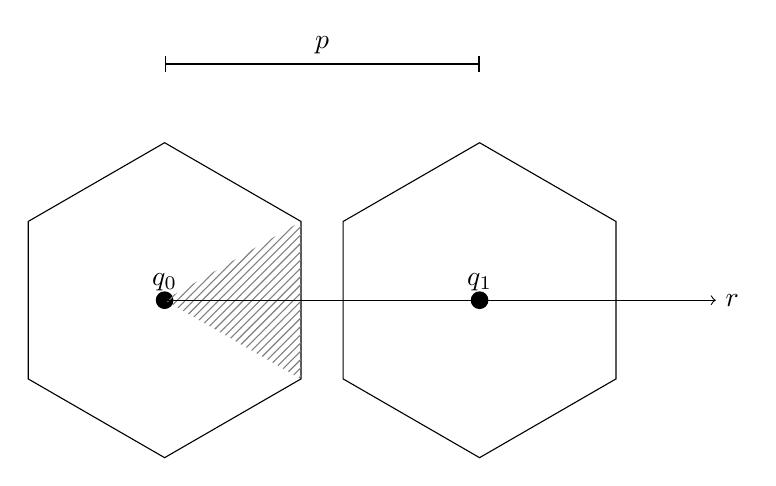
\begin{tikzpicture}[scale=4]
    \hexpix{\hexsize}
    \node[anchor=south] at (0, 0) {$q_0$};
    \begin{scope}
        \clip (0,0) -- (30:\hexsize) -- (-30:\hexsize) -- cycle;
        \fill[pattern=north east lines, pattern color=gray] (-1,-1) rectangle (1,1);
    \end{scope}
    \hexpix[xshift=1cm]{\hexsize}
    \node[anchor=south] at (1, 0) {$q_1$};
    \draw[|-|] (0, 0.75) -- (1, 0.75);
    \node[anchor=south] at (0.5, 0.75) {$p$};
    \draw[->] (0, 0) -- (1.75, 0);
    \node[anchor=west] at (1.75, 0) {$r$};
    \end{tikzpicture}
    \caption{Illustration of the two-pixel event topology. Assuming that  $q_1 \leq q_0$, 
    the hatched triangle represents the portion of the phase space in terms of the 
    true impact point originating this topology. The $r$ axis is where the event position is reconstructed.}
    \label{fig:two_pixel_event}
\end{figure}

The case of two-pixel events is more interesting, and it can be treated in a similar way as a microstrip detector. Considering the readout design of ASIX, where the triggering pixel is always located at the center of a seven pixel cluster, a small change in the definition of $\eta$ is necessary, which is now defined as
\begin{equation}
\eta = \frac{q_1}{q_0 + q_1},
\label{eq:eta_2pix}
\end{equation}
where $q_0$ is always the central pixel of the cluster and $q_1$ is one of the outer pixels. This means that for ASIX the definition of left and right has no more sense as in microstrips detector. This change in the definition affects the shape of the $\eta$ variable distribution, because now it ranges in the interval $(0, 0.5)$ and does not have a double peak as in Fig. \ref{fig:belau_eta}. 

Before calculating the $\eta$ distribution it is necessary to verify if two-pixel events are uniformly distributed along the axis that connects the two pixel centers shown in Fig. \ref{fig:two_pixel_event}. The scatter plot shown in Fig. \ref{fig:2pix_scatter} shows how the real impact position of two-pixel events are distributed. By observing the count distribution of these events projected onto the axes connecting the center of the central pixel with the outer ones, shown in Fig. \ref{fig:2pix_scatter} as well, it is possible to see that the events are not uniformly distributed.

\begin{figure}
    \centering
    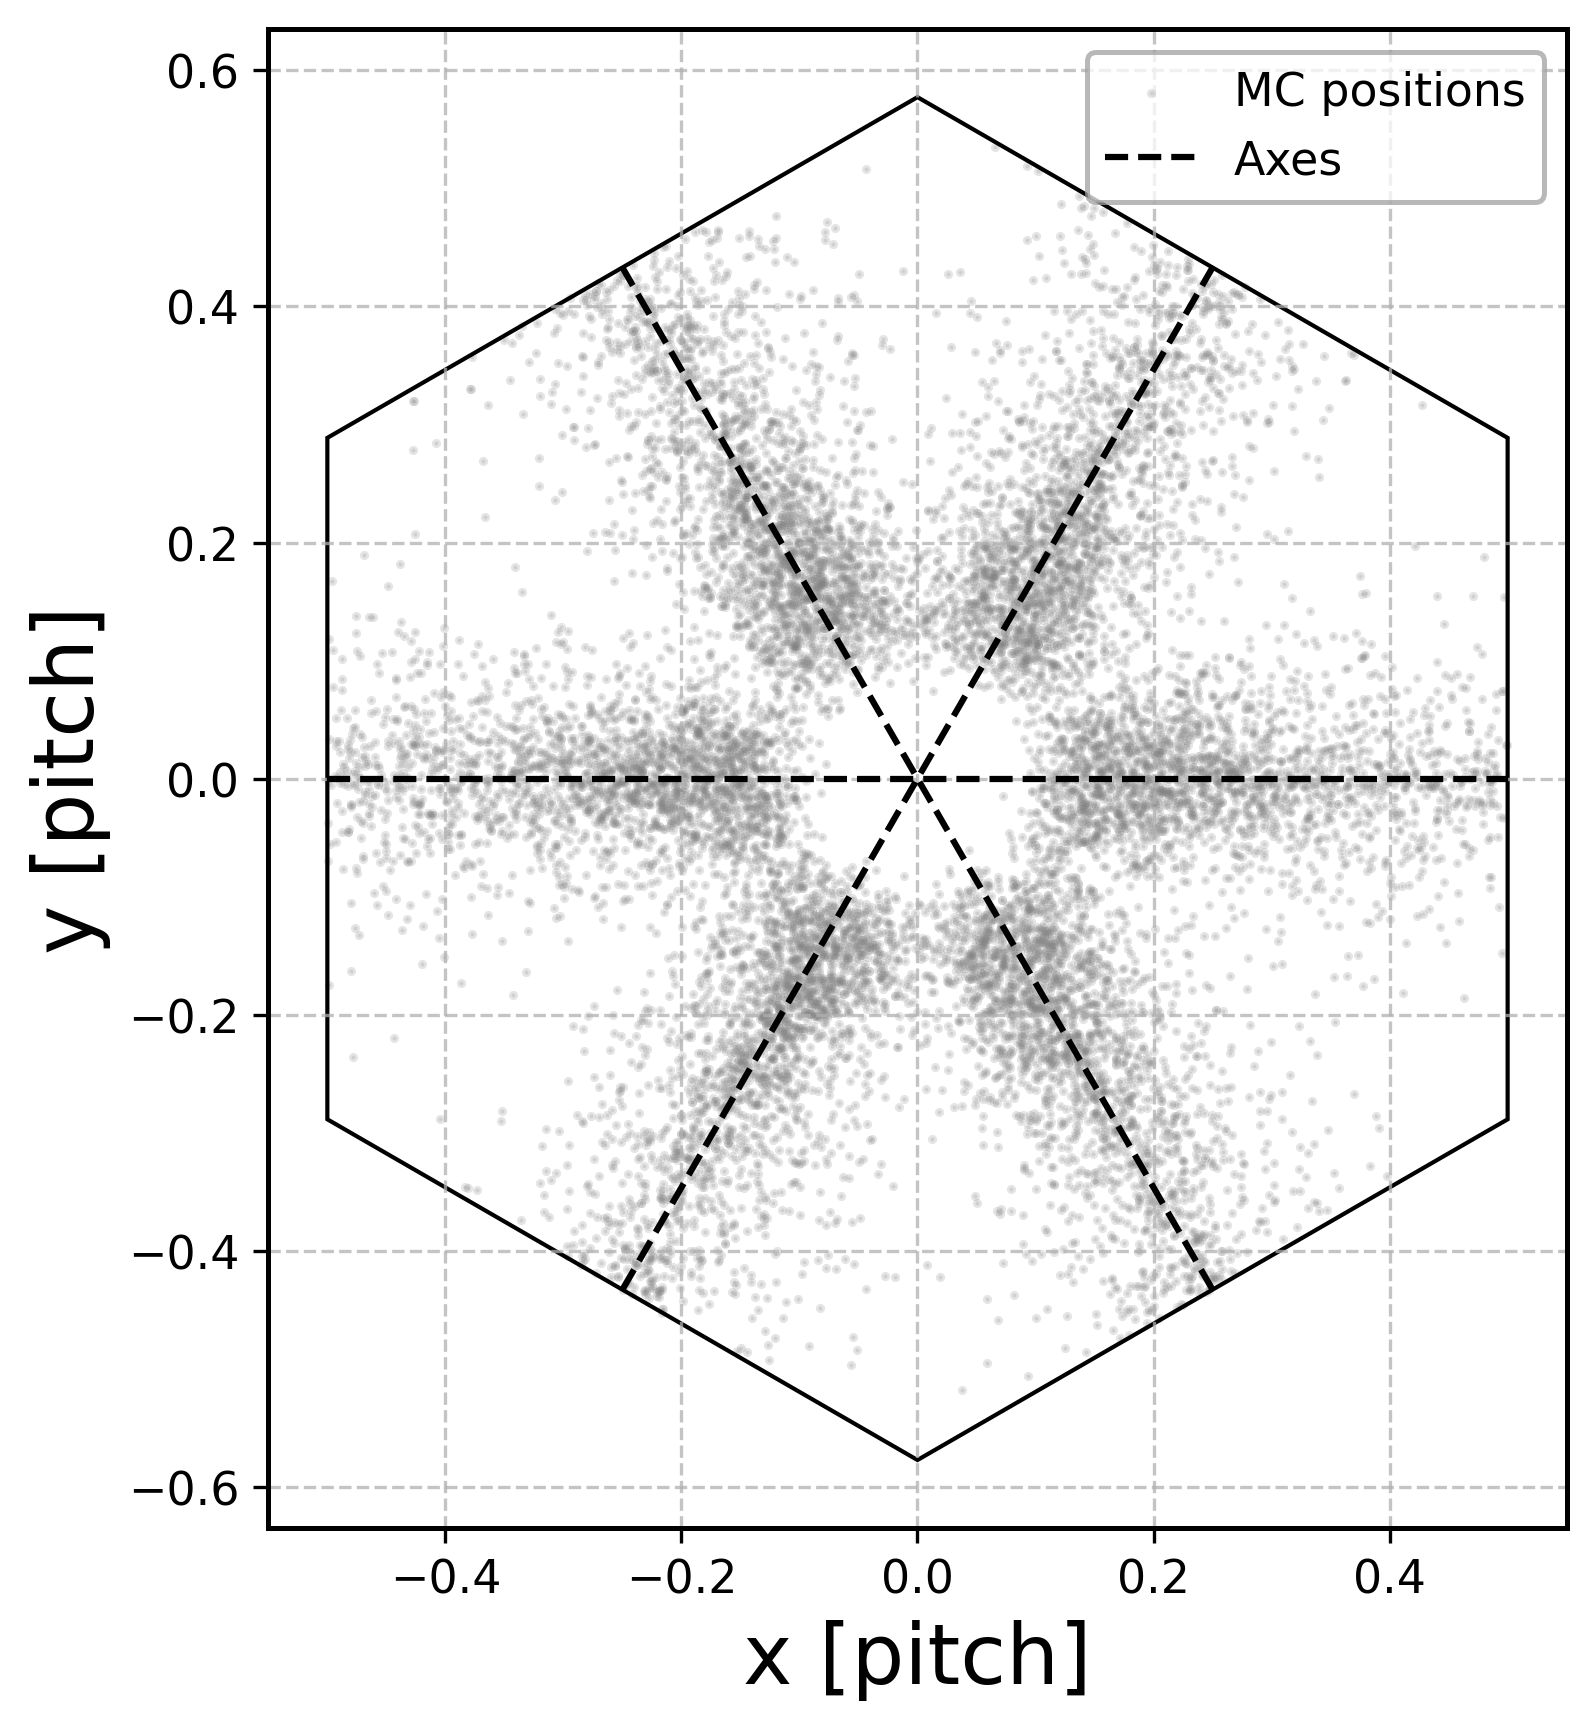
\includegraphics[width=0.35\linewidth]{figures/chapter4/position/eta_2pix_scatter}
    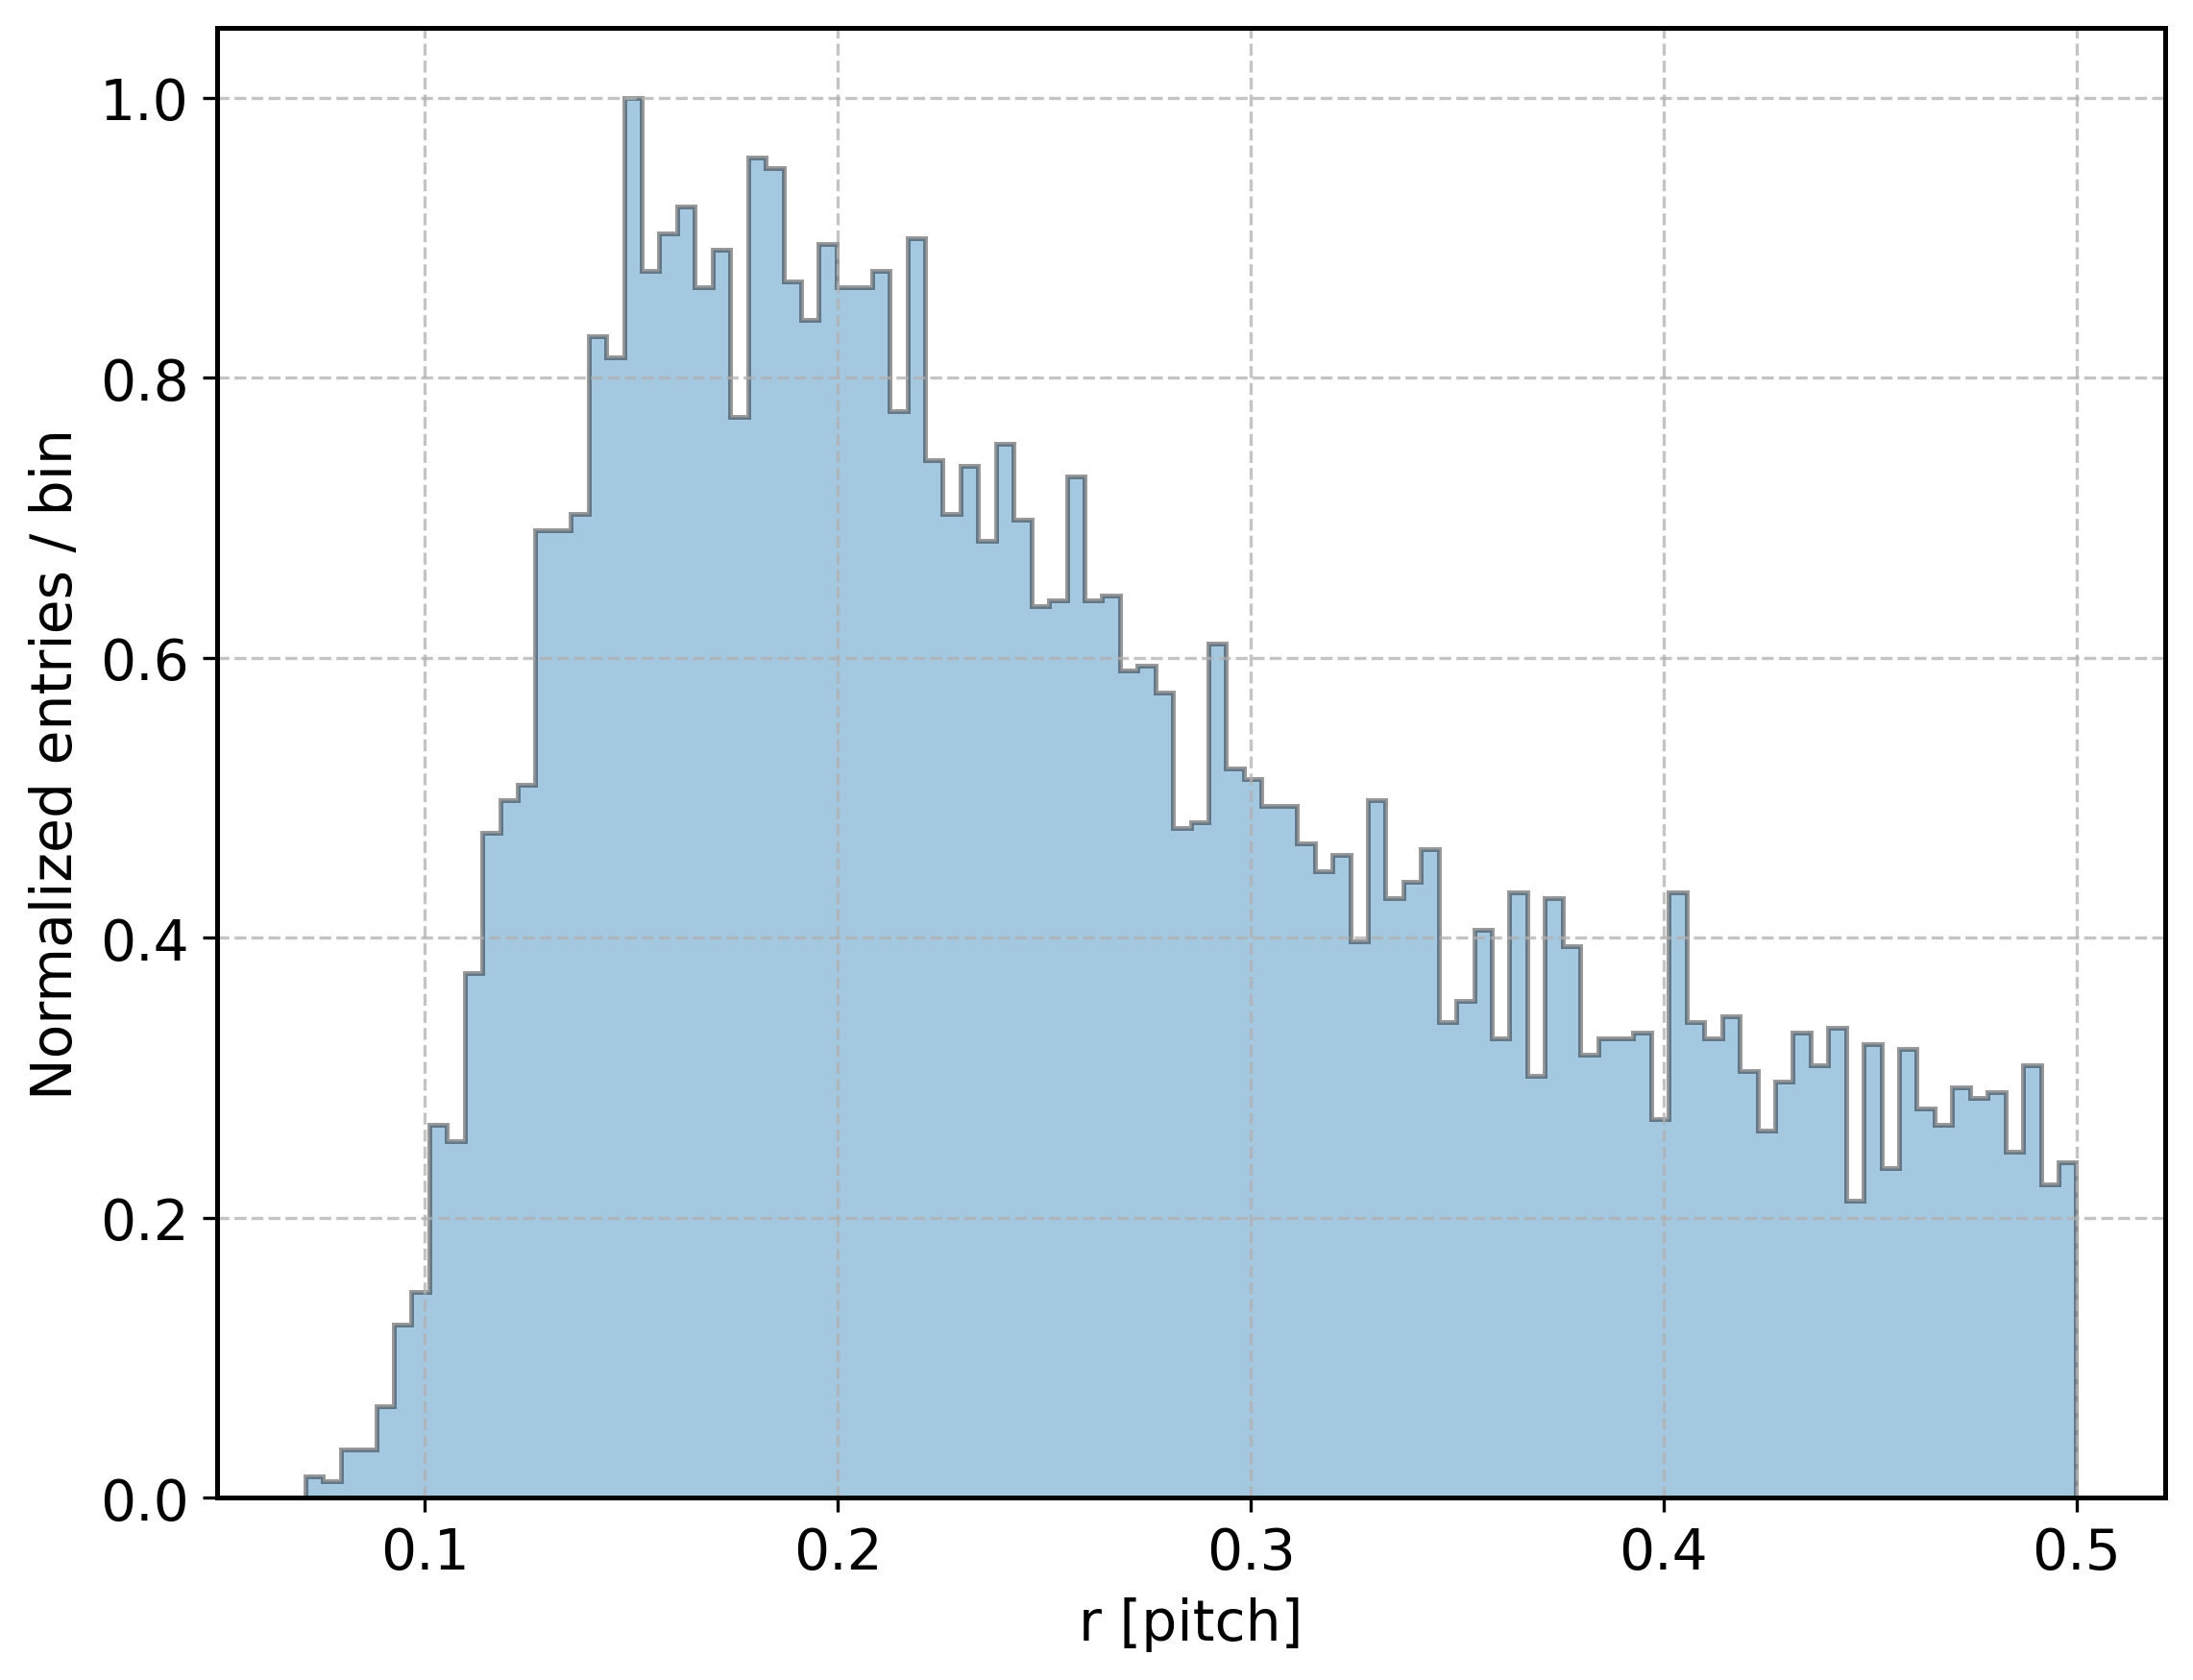
\includegraphics[width=0.49\linewidth]{figures/chapter4/position/eta_2pix_dr_hist}
    \caption{Scatter plot of Monte Carlo truth impact positions of two-pixel events on the central pixel (left panel) and event count distribution of the events projected onto the relevant axes, shown with dashed lines (right panel).}
    \label{fig:2pix_scatter}
\end{figure}
%
%To apply the geometrical correction to the $\eta$ distribution, an iterative procedure is adopted. In the initial step, the relationship between $\eta$ and the position $r$ is assumed to be linear, mapping the minimum and maximum observed values of $\eta$ to the boundaries of the $r$ interval. Using this preliminary $r(\eta)$ mapping, the $\eta$ distribution is corrected by weighting the counts in each $\eta$ bin by the inverse of the spatial density at the corresponding position $r$. The cumulative distribution function of this weighted $\eta$ histogram is then calculated, yielding an updated, non-linear calibration function $r(\eta)$. This new mapping is fed back into the previous step to re-evaluate the weights for the next iteration. The process is repeated until the relation $r(\eta)$ converges to a stable shape. The resulting distributions are shown in Fig. \ref{fig:eta_2pix}. For the final event reconstruction, the cumulative distribution is interpolated to obtain a continuous function $r(\eta)$.
%

To apply the geometrical correction on the $\eta$ distribution, an iterative approach can be adopted. Calling $g(\eta)$ the measured $\eta$ distribution and $\rho(r)$ the event spatial distribution along the reconstruction axis $r$. In the first step $n=0$, the relation between $\eta$ and $r$ is assumed to be linear, and the minimum and maximum observed values of $\eta$ correspond to the minimum and maximum values of $r$

\begin{equation}
r_0(\eta) = r_{\textrm{min}} + (\eta - \eta_{\textrm{min}}) \frac{r_{\textrm{max}} - r_{\textrm{min}}}{\eta_{\textrm{max}} - \eta_{\textrm{min}}}.
\end{equation}

At a generic step $n$, using the relation $r_n(\eta)$ found in the previous iteration, the corrected distribution $g_{n+1}(\eta)$ is calculated. This is done by weighting the original distribution with the inverse of the spatial density evaluated at that position

\begin{equation}
g_{n+1}(\eta) = \frac{g(\eta)}{\rho(r_n(\eta))}.
\end{equation}

\begin{figure}[!b]
    \centering
    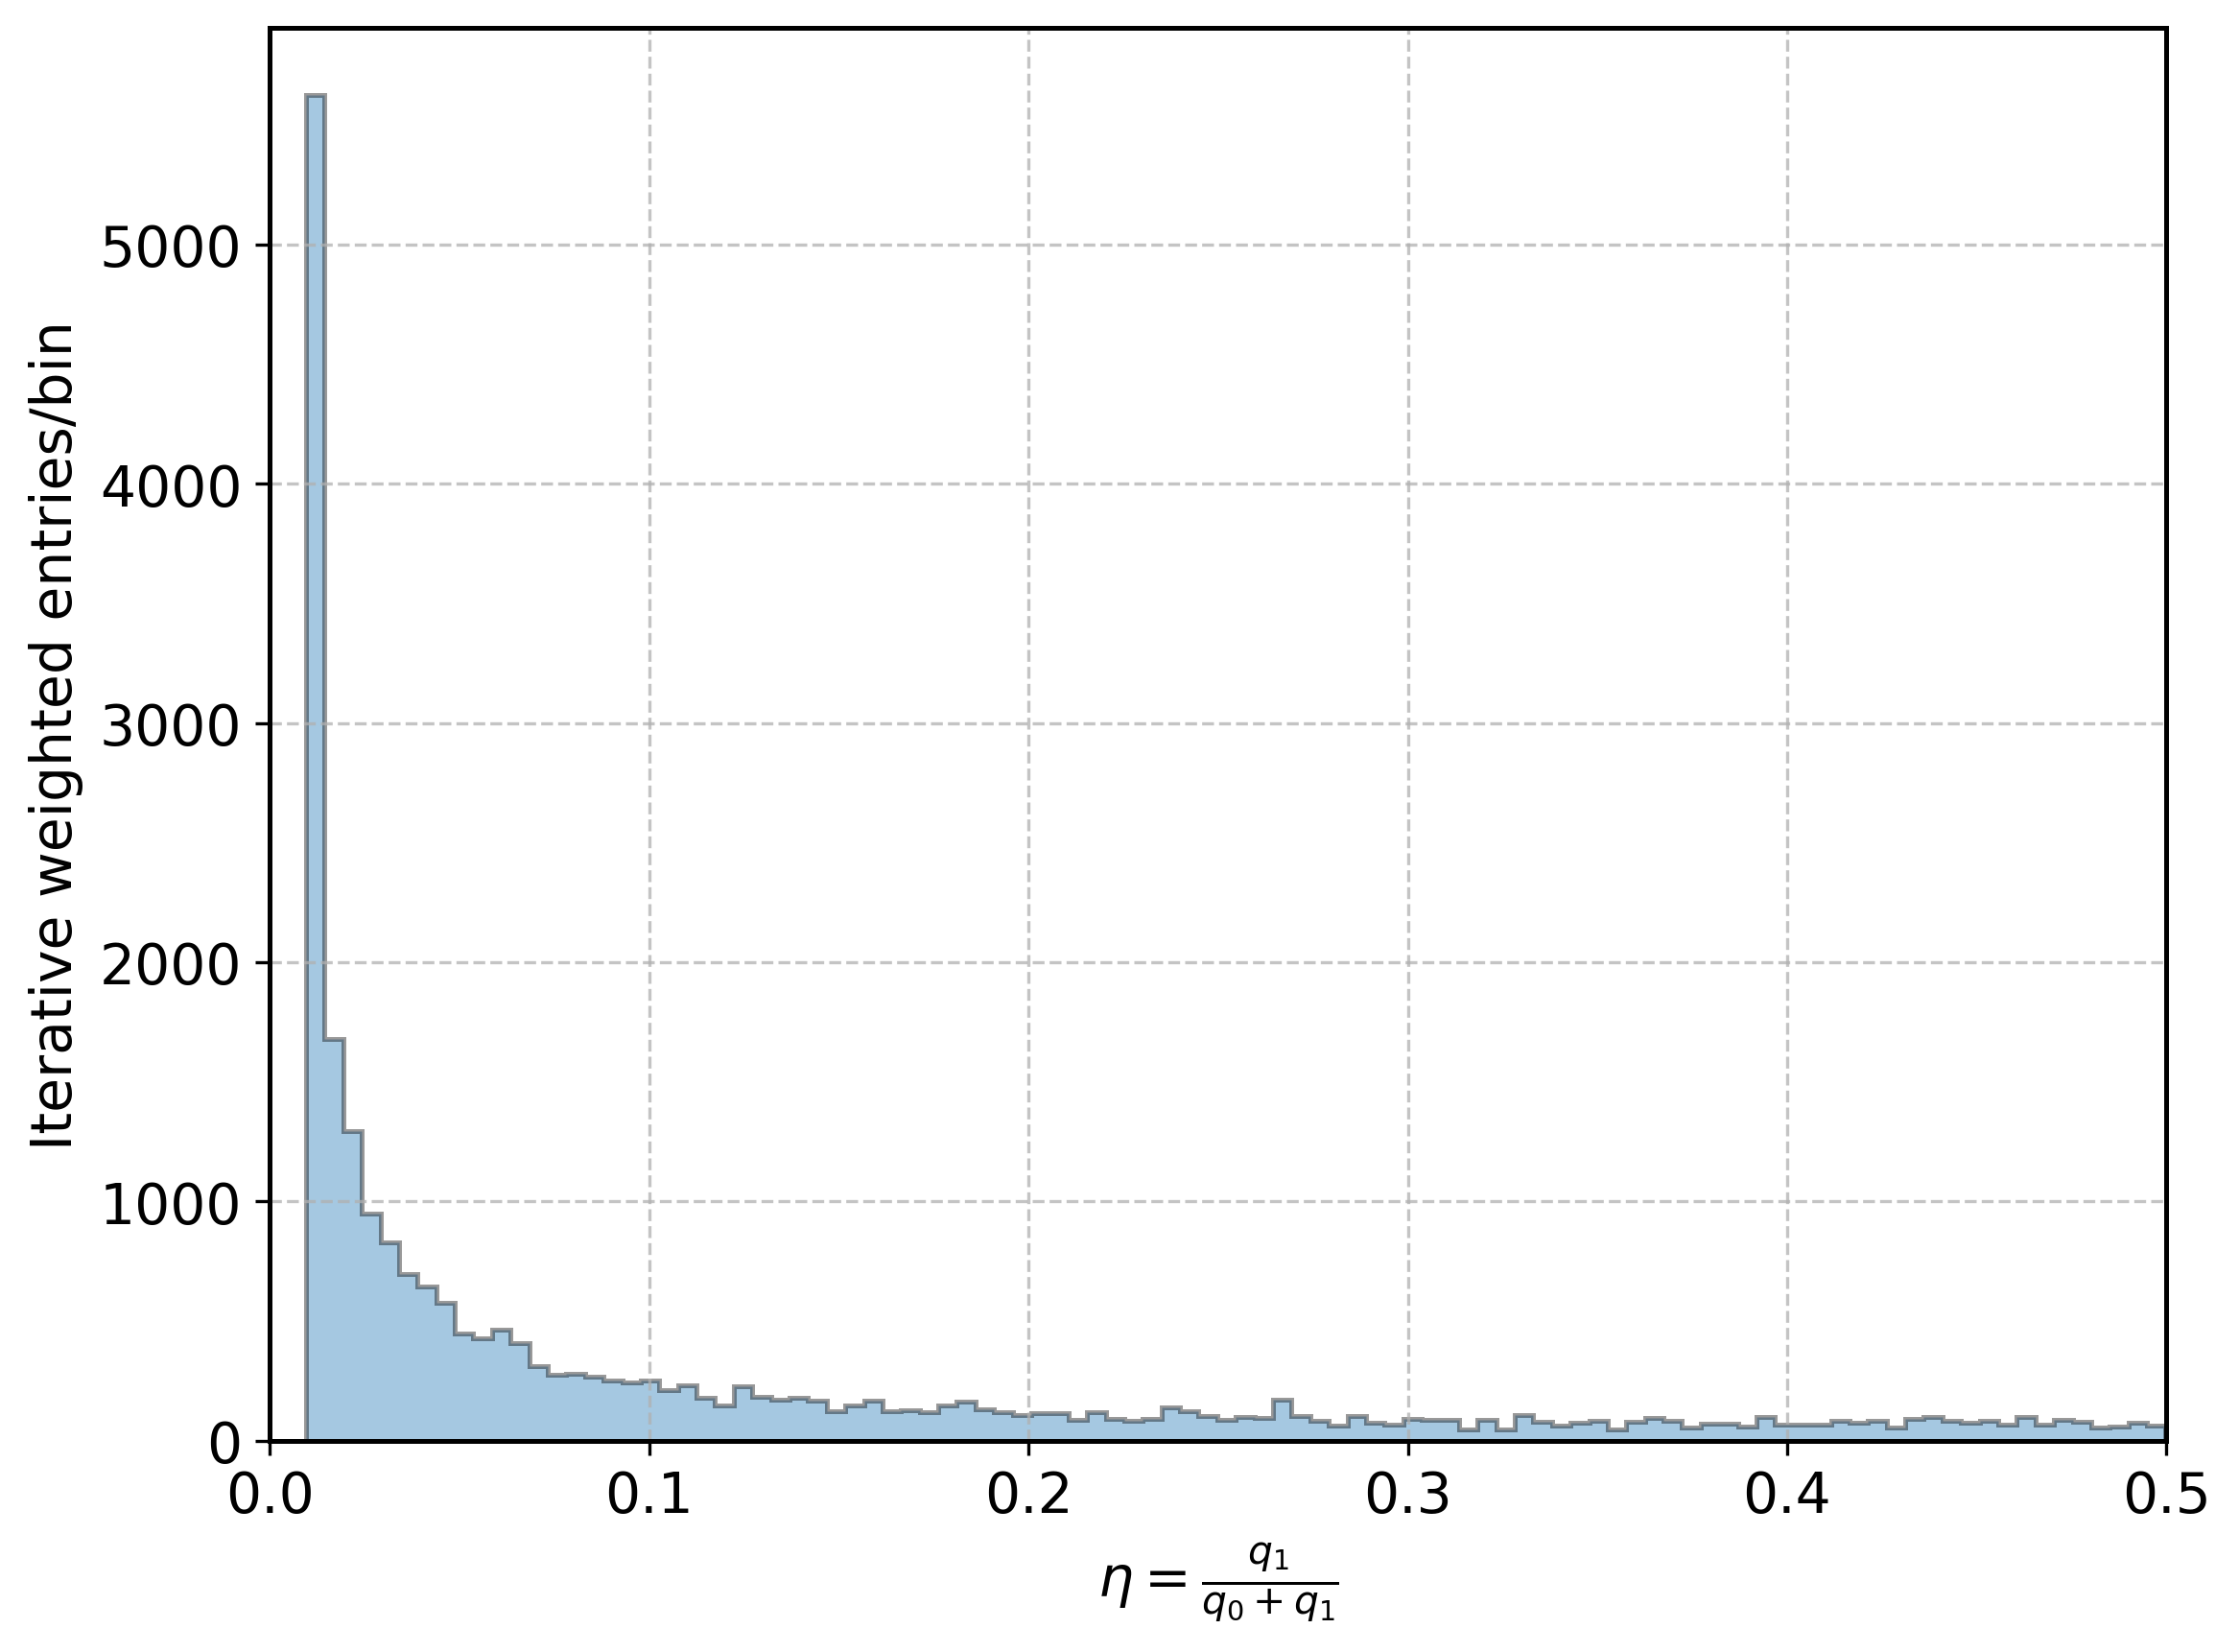
\includegraphics[width=0.49\linewidth]{figures/chapter4/position/eta_hist}
    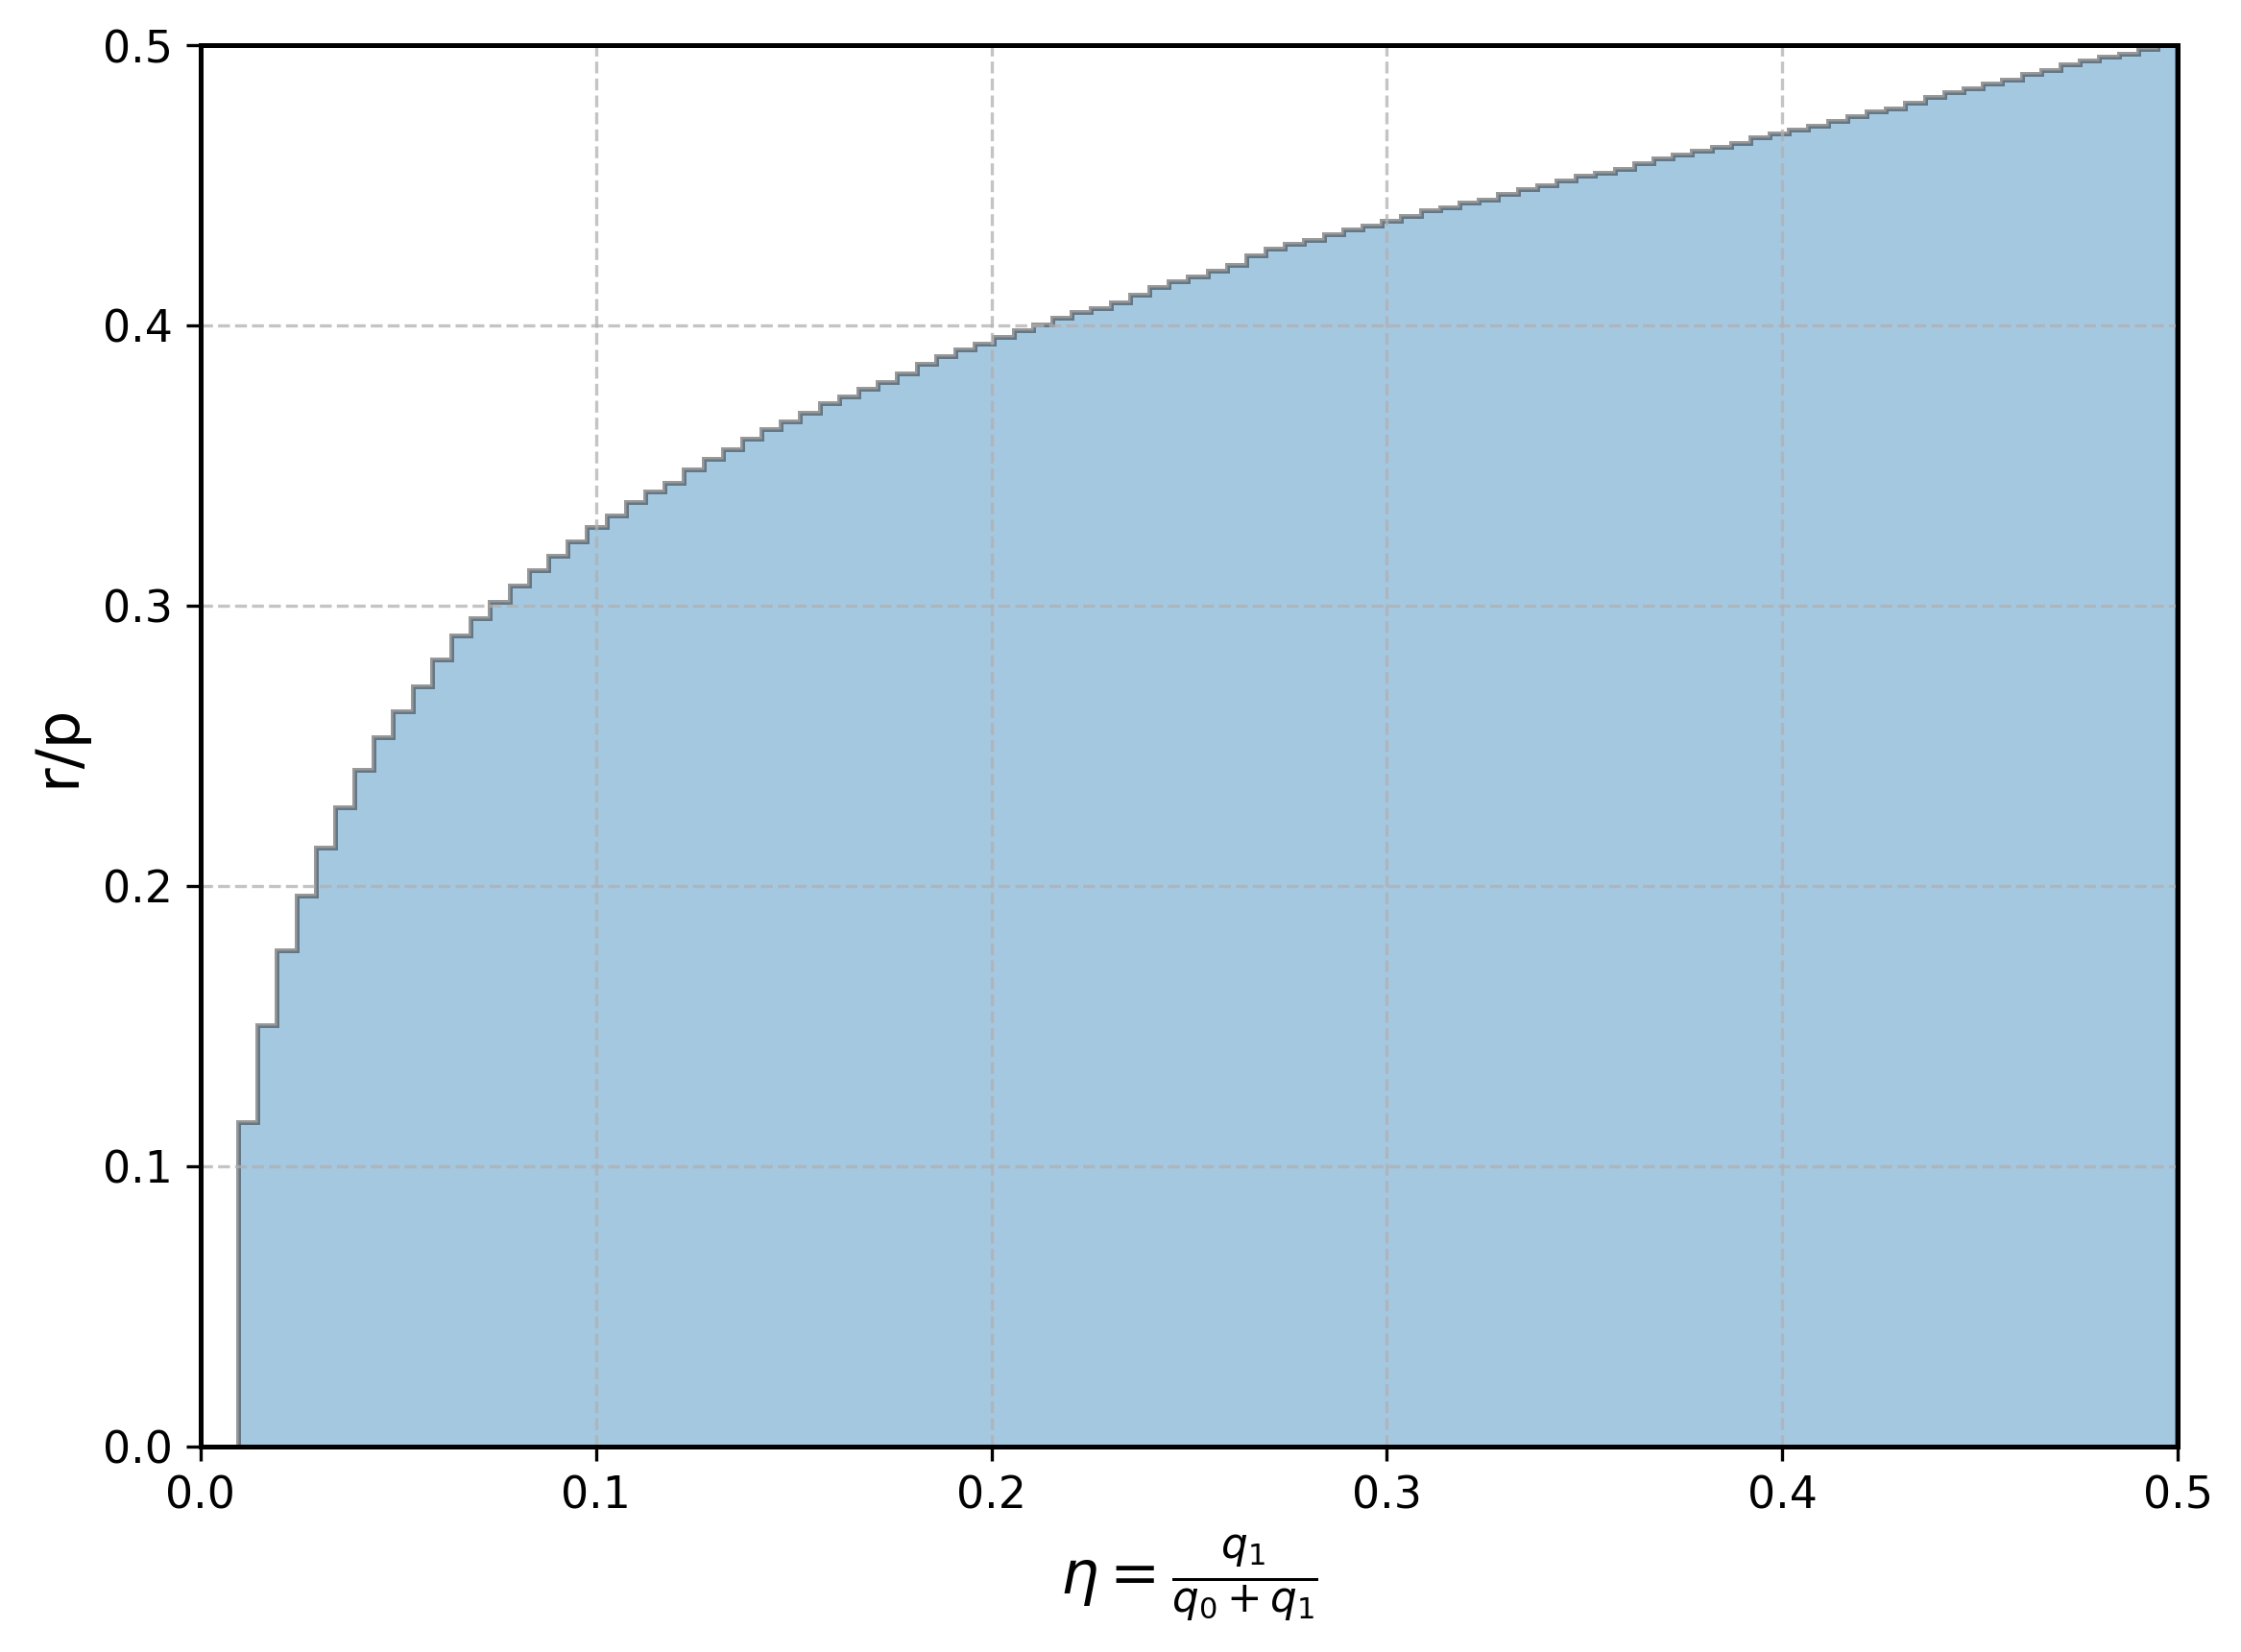
\includegraphics[width=0.49\linewidth]{figures/chapter4/position/eta_cumulative}
    \caption{$\eta$ distribution (left panel) after correcting for non-uniformity of event distribution and its cumulative distribution (right panel) for two-pixel events. The two distributions are truncated near $\eta=0$ because of a zero-suppression threshold that is applied.}
    \label{fig:eta_2pix}
\end{figure}

The cumulative distribution of this weighted histogram is calculated, which gives the updated non-linear relation $r_{n+1}(\eta)$

\begin{equation}
r_{n+1}(\eta) = r_{\textrm{min}} + (r_{\textrm{max}} - r_{\textrm{min}}) \frac{\int_{\eta_{\textrm{min}}}^{\eta} g_{n+1}(\eta') \, d\eta'}{\int_{\eta_{\textrm{min}}}^{\eta_{\textrm{max}}} g_{n+1}(\eta') \, d\eta'}.
\end{equation}

Using this relation, the steps are repeated. The resulting distributions are shown in Fig. \ref{fig:eta_2pix}. Finally, for event reconstruction, the cumulative distribution is interpolated to get a continuous function $r(\eta)$.

This approach can be generalized to the case of three-pixels events as well. Contrary to the two-pixels case, this is a two-dimensional problem. A single $\eta$ variable is not enough and the generalization of the previous case is to define the variables

\begin{equation}
\eta_1 = \frac{q_1}{q_0 + q_1 + q_2}, \quad \quad \eta_2 = \frac{q_2}{q_0 + q_1 + q_2}, \quad \quad q_0 > q_1 > q_2.
\label{eq:eta_3pix}
\end{equation}

\begin{figure}[!b]
    \centering
    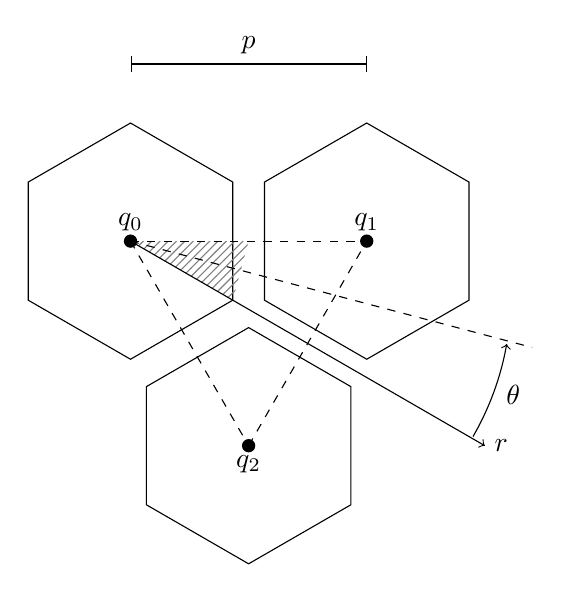
\begin{tikzpicture}[scale=3]
    \hexpix{\hexsize}
    \node[anchor=south] at (0, 0) {$q_0$};
    \draw[|-|] (0, 0.75) -- (1, 0.75);
    \node[anchor=south] at (0.5, 0.75) {$p$};
    \begin{scope}
        \clip (0,0) -- (0:\hexsize) -- (-30:\hexsize) -- cycle;
        \fill[pattern=north east lines, pattern color=gray] (-1,-1) rectangle (1,1);
    \end{scope}
    \hexpix[xshift=1cm]{\hexsize}
    \node[anchor=south] at (1, 0) {$q_1$};
    \hexpix[xshift=0.5cm, yshift=-0.866cm]{\hexsize}
    \node[anchor=north] at (0.5, -0.866) {$q_2$};
    \draw[dashed] (0, 0) -- (1, 0);
    \draw[->] (0, 0) -- (1.5, -0.866);
    \draw[dashed] (0, 0) -- (0.5, -0.866);
    \draw[dashed] (0.5, -0.866) -- (1, 0);
    \draw[dashed] (0, 0) -- (1.7, -0.45);
    \node[anchor=west] at (1.5, -0.866) {$r$};
    \draw[->] (1.45, -0.827) arc[start angle=-30, end angle=-10, radius=1.2];
    \node[anchor=west] at (1.55, -0.65) {$\theta$};
    \end{tikzpicture}
    \caption{Illustration of the three-pixel event topology. Assuming that the ordering
    of the charges is $q_2 \leq q_1 \leq q_0$, the hatched triangle represents again the 
    portion of the phase space in terms of the true impact point originating this topology.}
    \label{fig:three_pixel_event}
\end{figure}

These two new variables are still not good enough, because it is not easy to parametrize the geometry of the problem with them. By looking at the geometry of the three pixels in Fig. \ref{fig:three_pixel_event}, a better parametrization can be employed to simplify the description of this type of events.

The idea is to decompose the two-dimensional problem into two one-dimensional problems that can be treated as two-pixel events, each describing a specific coordinate. The best coordinates for this problem 
are a radial coordinate and an angular coordinate. The two coordinates are defined as follows:
\begin{itemize}[label=-]
\item $r$ is distance of the incident position projected onto the axis that passes through the vertex of the central pixel and the middle point between the outer pixels centers;
\item $\theta$ is the angle measured starting from the latter axis and oriented towards the outer pixel with the highest charge collected.
\end{itemize}

Considering the ASIX readout geometry, where the central pixel is always the one with the highest pixel and the other two pixels are neighbors, the radial component can be parametrized as a two-pixel event by considering the outer pixels as a single pixel with charge equal to their sum. This automatically defines a new $\eta_+$ variable which is defined as

\begin{equation}
\eta_+ = \eta_1 + \eta_2.
\label{eq:eta_sum}
\end{equation}

\begin{figure}[!t]
    \centering
    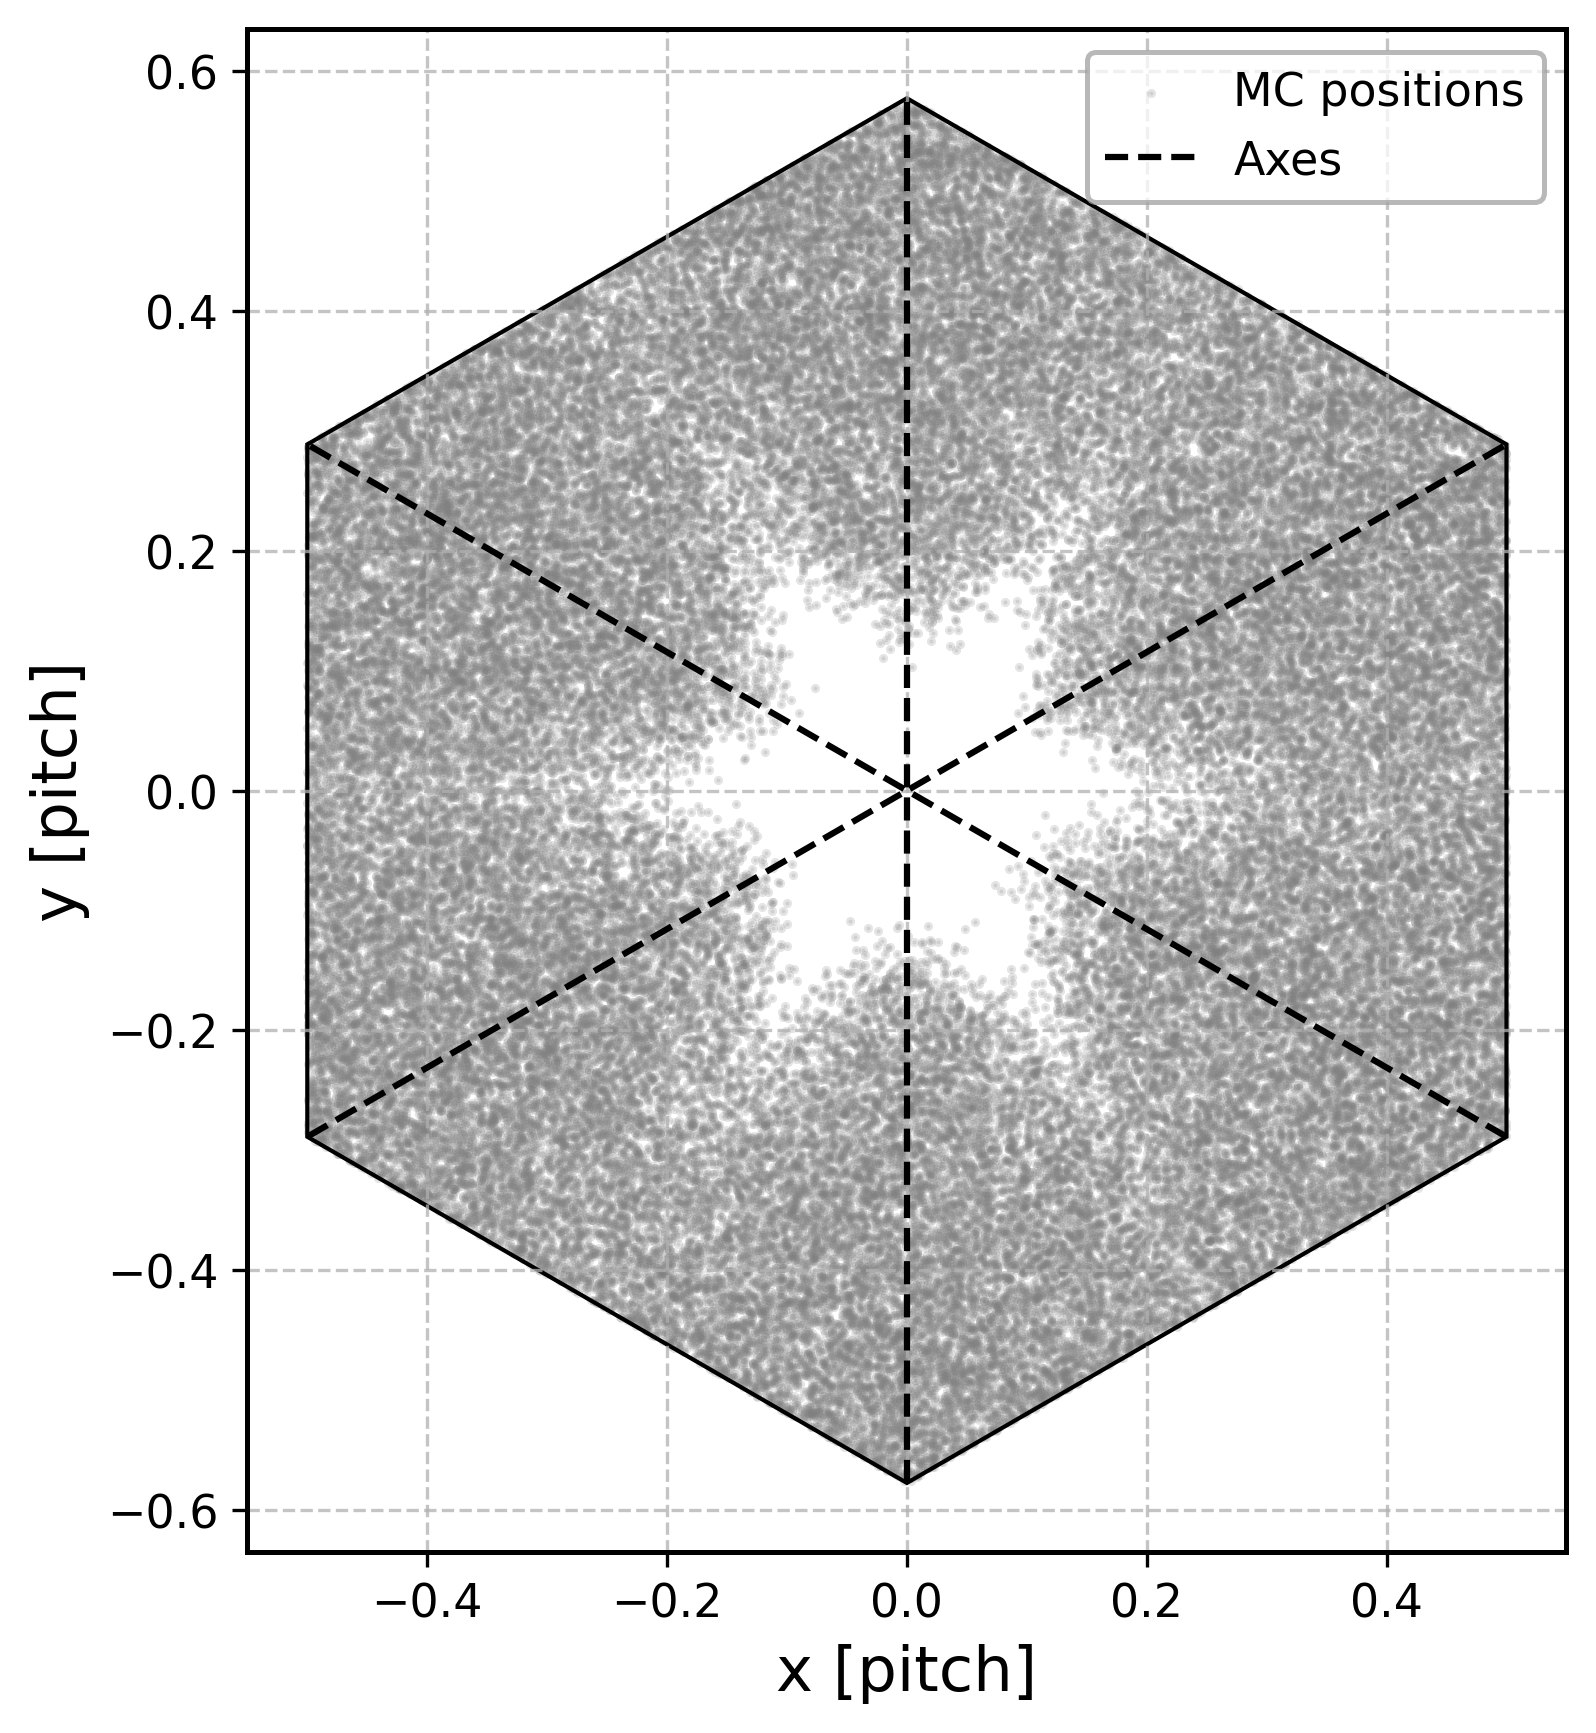
\includegraphics[width=0.35\linewidth]{figures/chapter4/position/eta_3pix_scatter}
    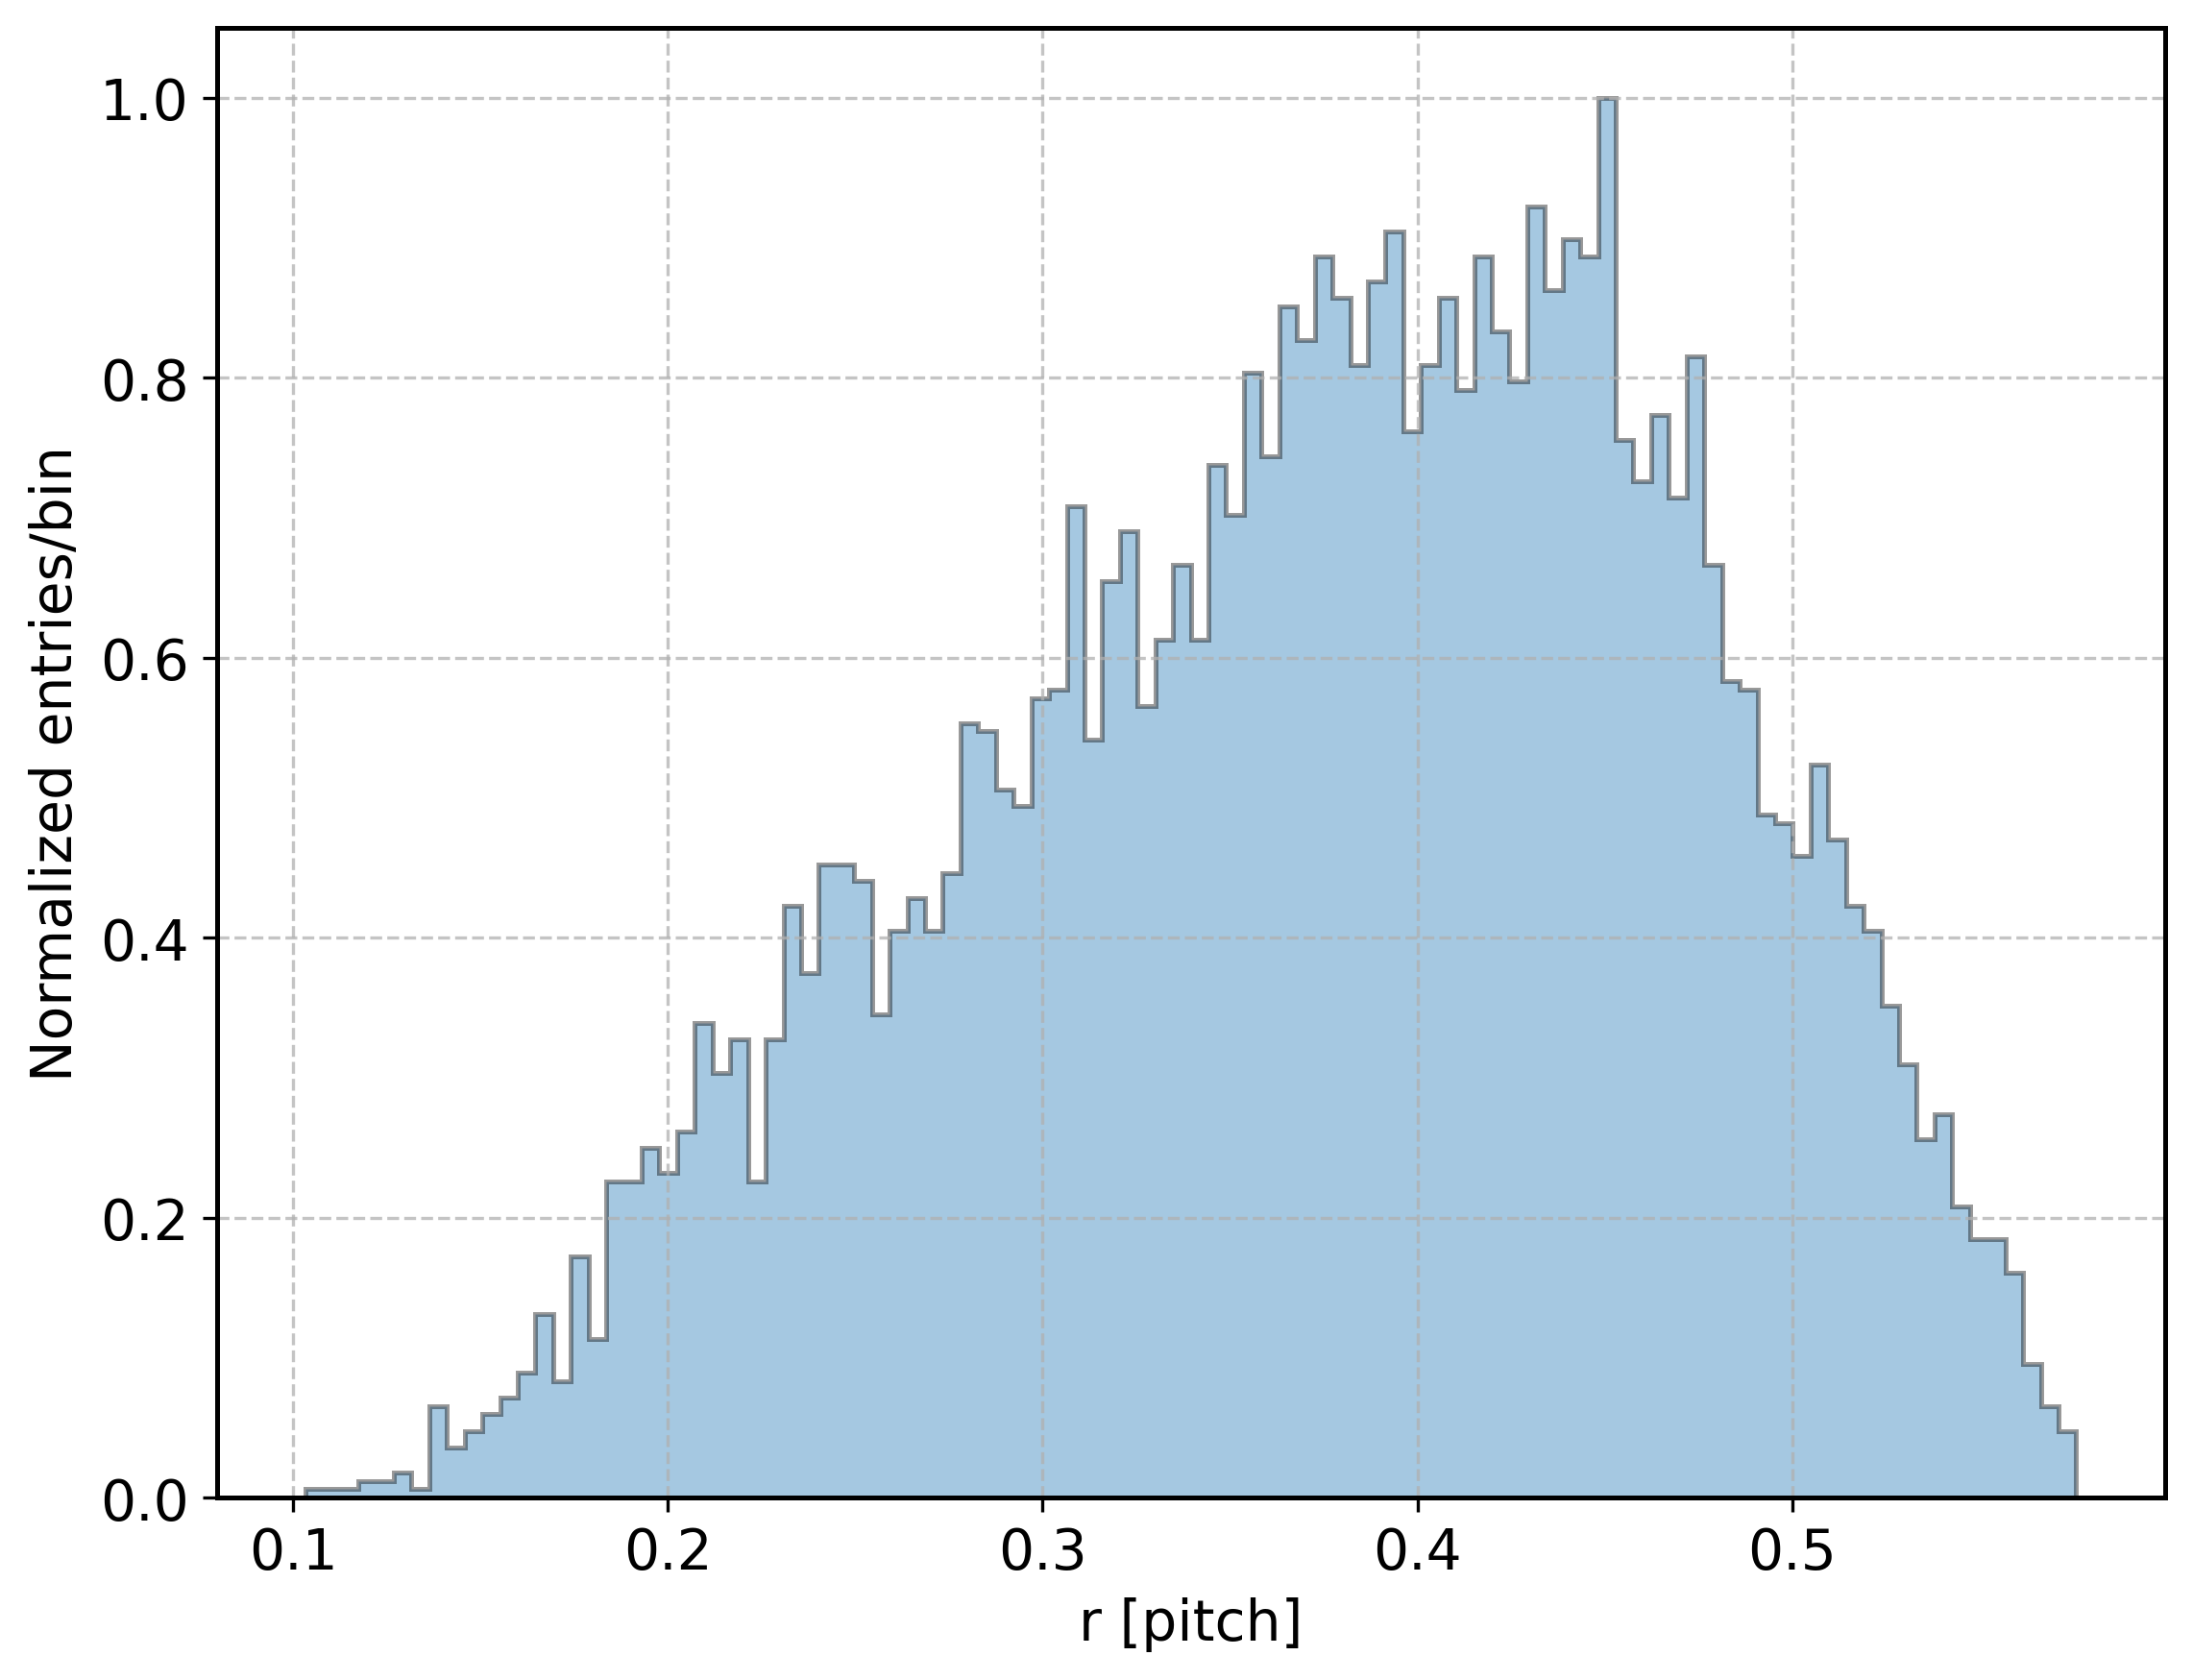
\includegraphics[width=0.49\linewidth]{figures/chapter4/position/eta_3pix_dr_hist}
    \caption{Scatter plot of Monte Carlo truth impact positions of three-pixel events on the central pixel (left panel) and event count distribution of the events projected onto the radial axes, shown with dashed lines (right panel). The empty circular region at the center of the hexagon is where events are labeled as one-pixel events, and its radius depends on the zero-suppression threshold.}
    \label{fig:3pix_scatter}
\end{figure}

The angular coordinate can be parametrized as a two-pixel event problem as well. In this case the relevant property is how the charge collected by the outer pixels is divided between them. As a consequence, a new variable can be defined as

\begin{equation}
\eta_- = \frac{\eta_1 - \eta_2}{\eta_+}.
\label{eq:eta_minus}
\end{equation}

\begin{figure}[!b]
    \centering
    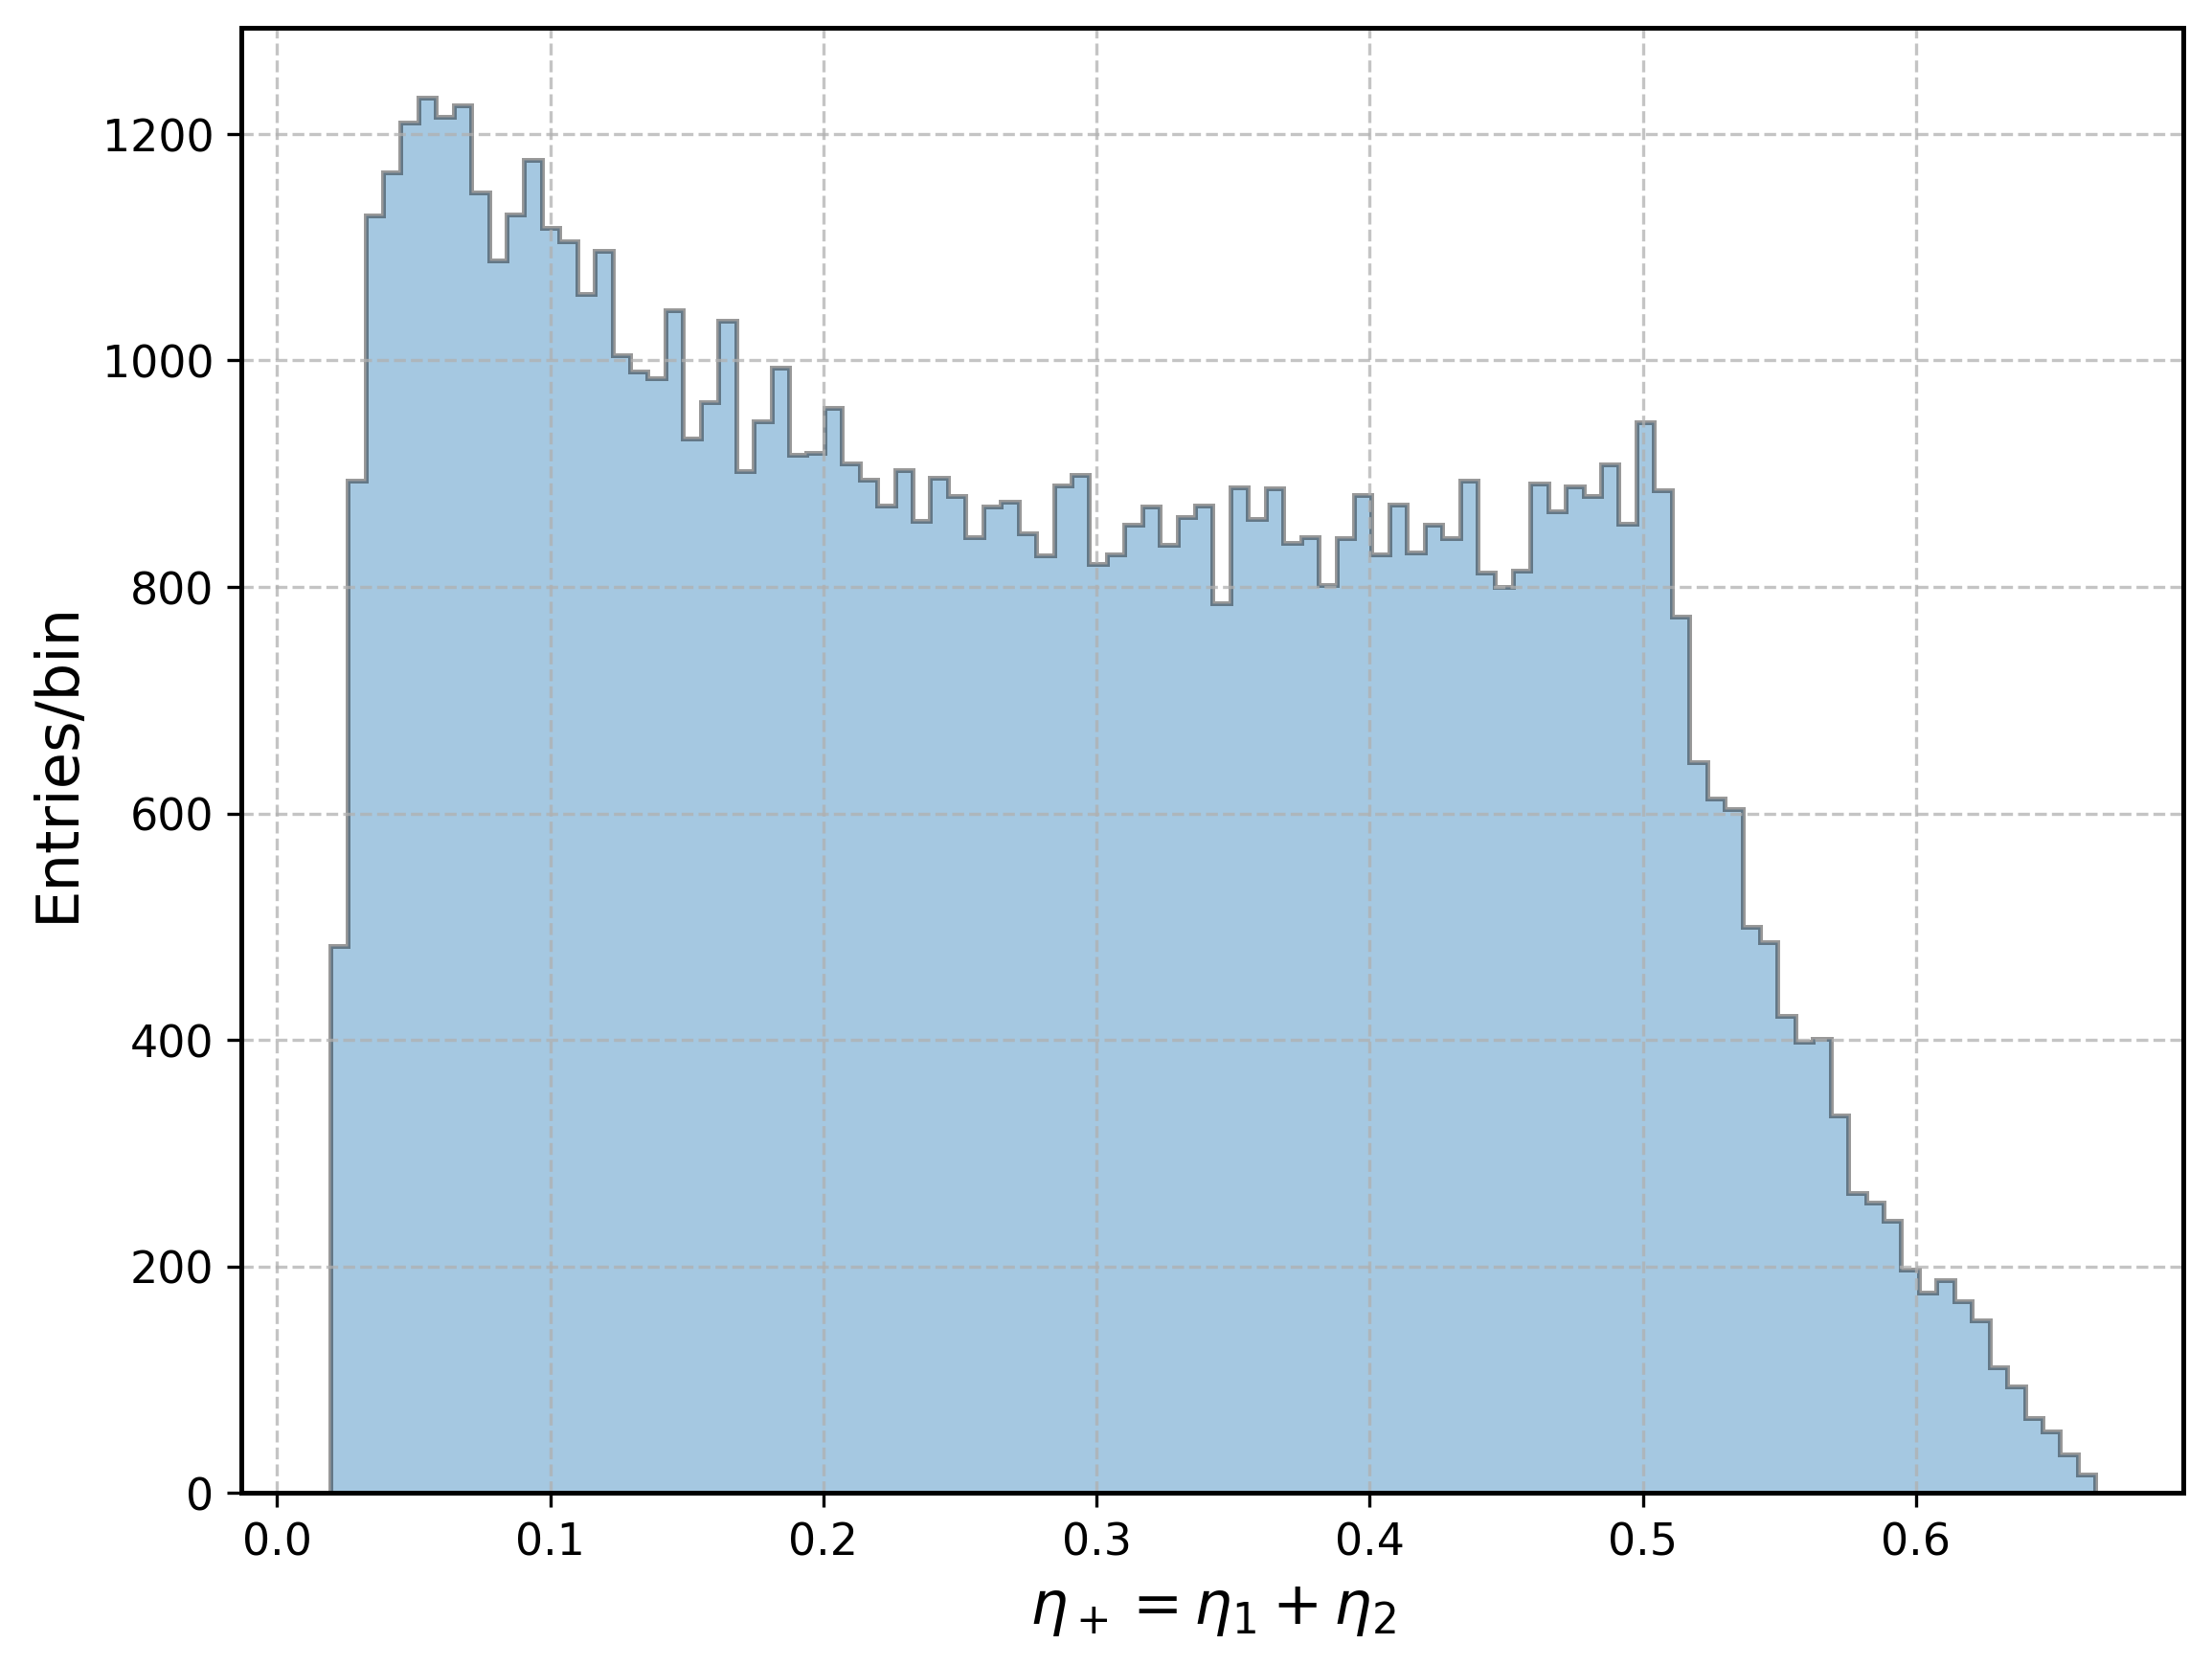
\includegraphics[width=0.49\linewidth]{figures/chapter4/position/eta_3pix_uncorrected_hist}
    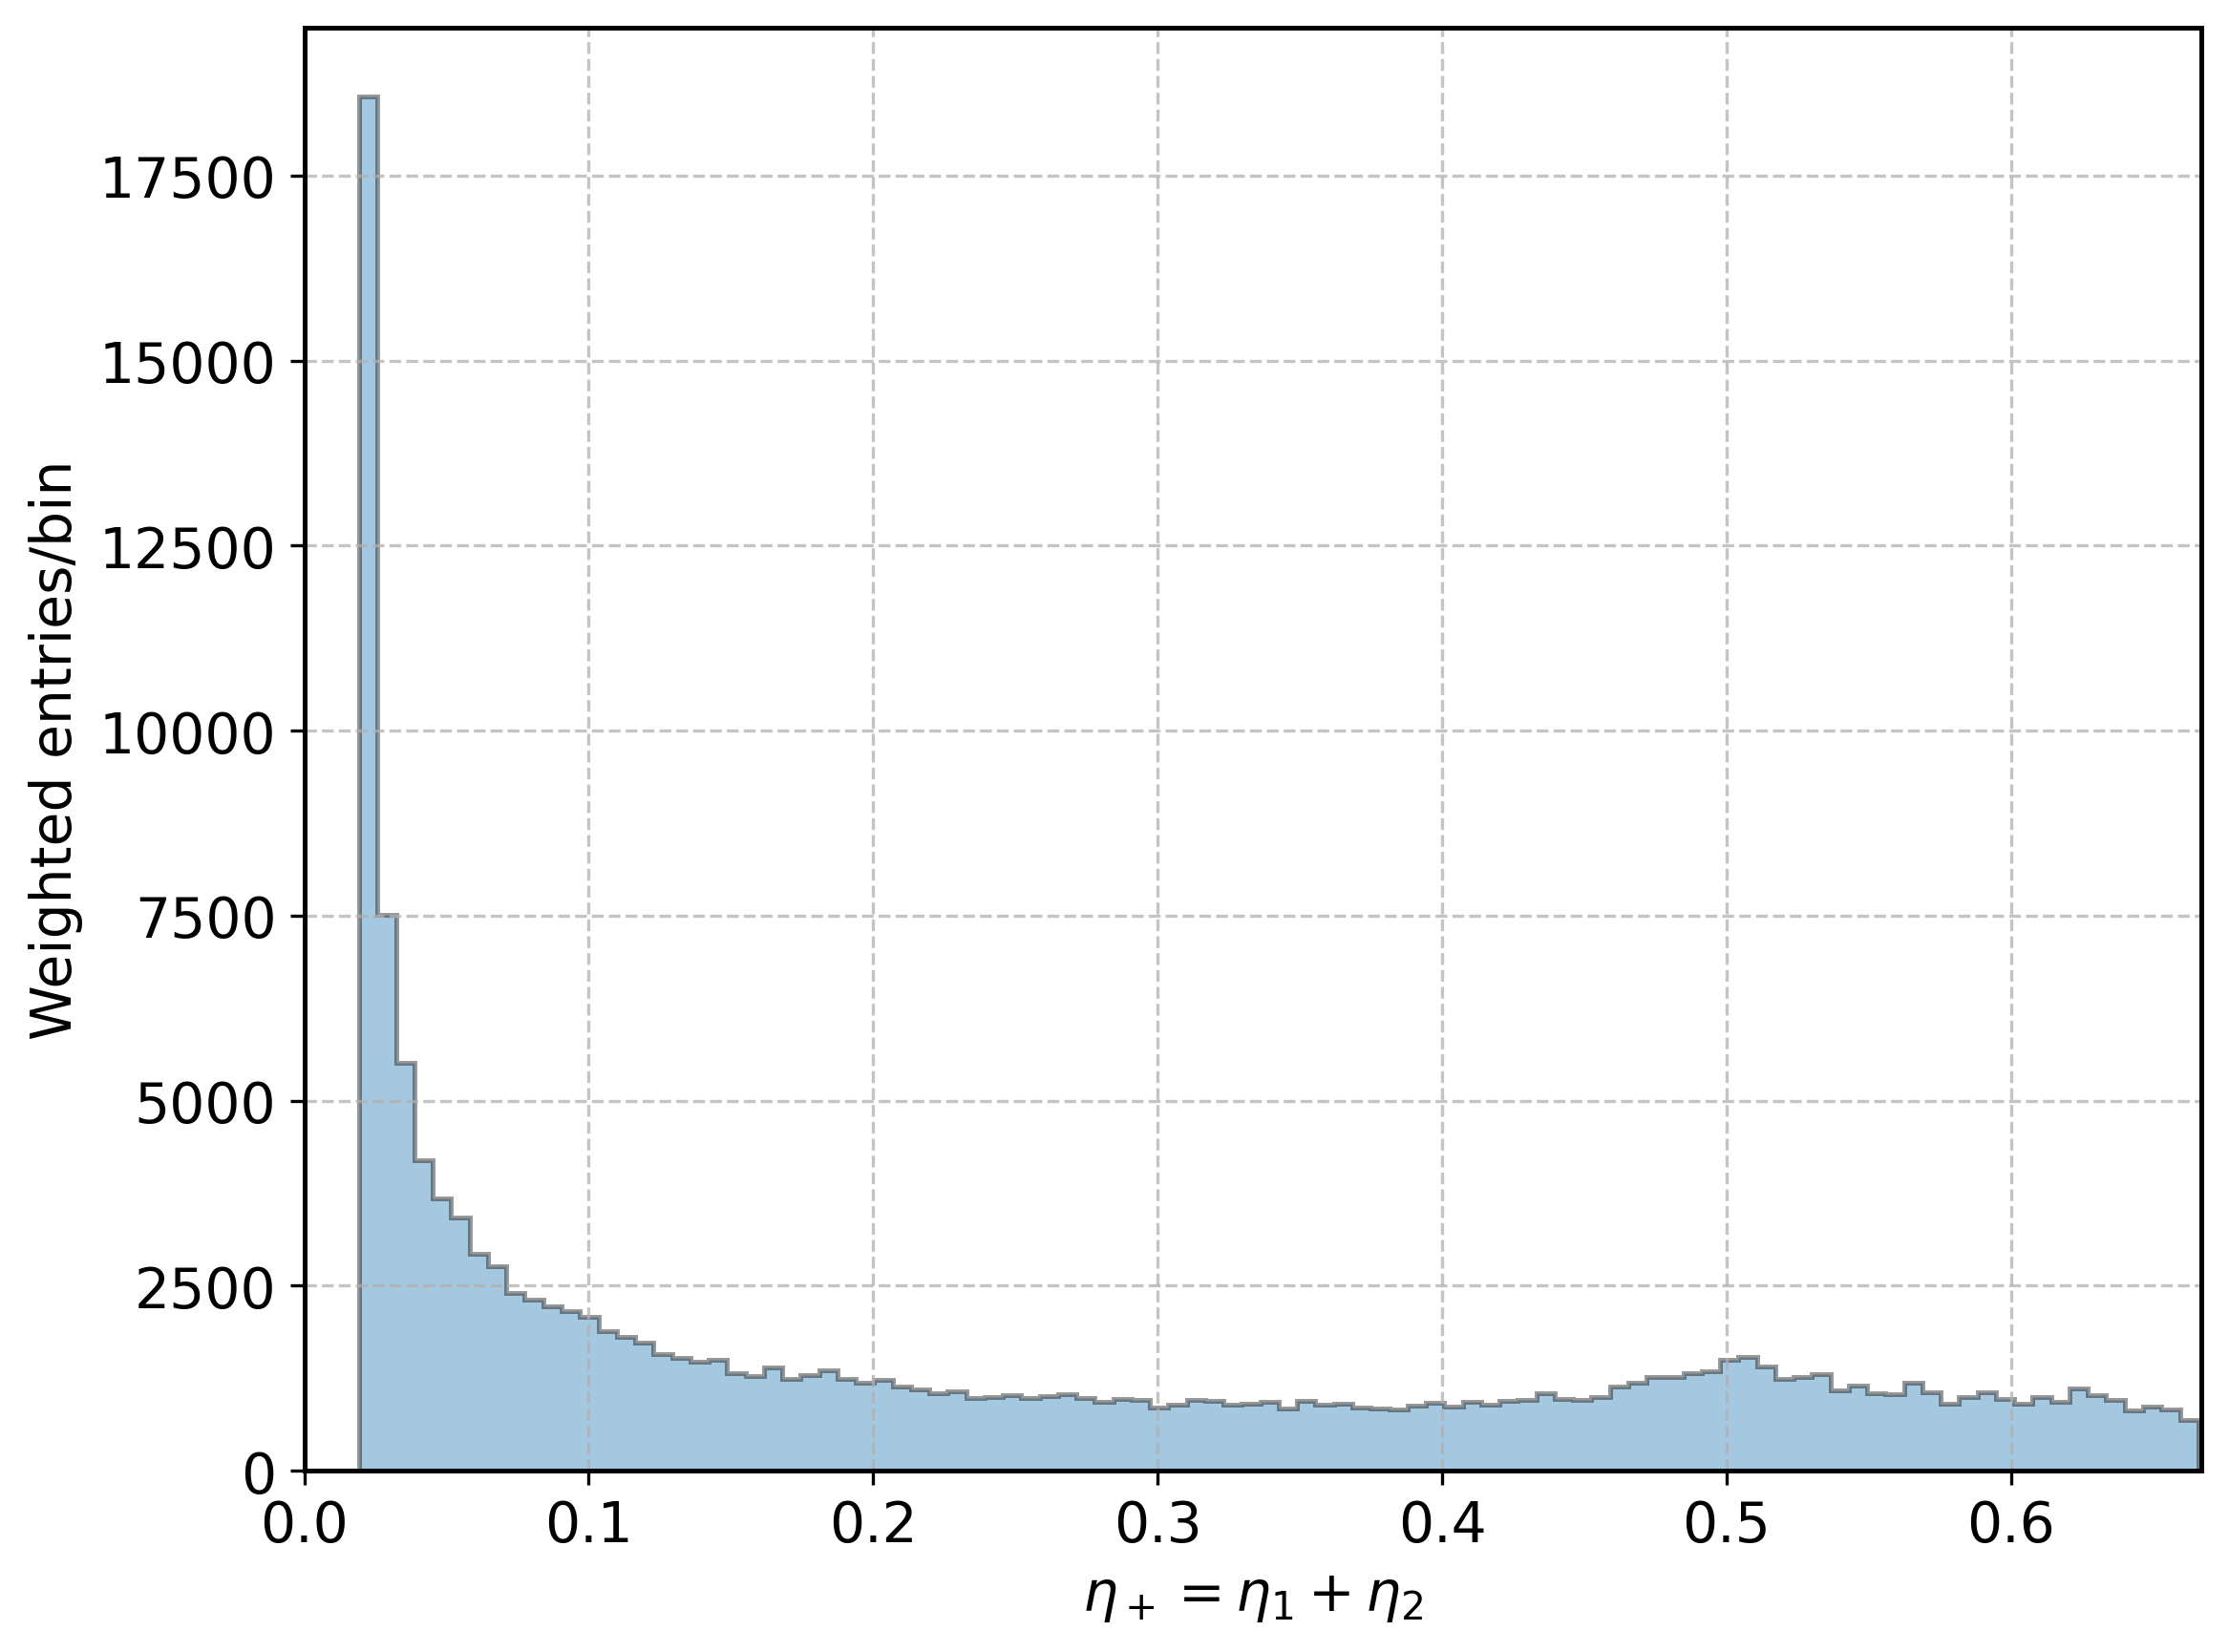
\includegraphics[width=0.49\linewidth]{figures/chapter4/position/eta_3pix_rad_hist}
    \caption{$\eta_+$ distribution without weigthing the entries to correct for non-uniformity (left panel) and distribution with the correction applied (right panel). $\eta_-$ distribution is not shown, but the distorsion in the uncorrected distribution is of a similar magnitude.}
    \label{fig:3pix_rad_eta}
\end{figure}

As in the case of two-pixel events, the uniformity of the events along the relevant axes has to be verified and, in case, corrected. The scatter plot of the Monte Carlo truth incidence positions and their distribution along the radial axis for three-pixel events are shown in Fig. \ref{fig:3pix_scatter}. It is possible to see that the distribution is highly non-uniform.

\begin{figure}[!t]
    \centering
    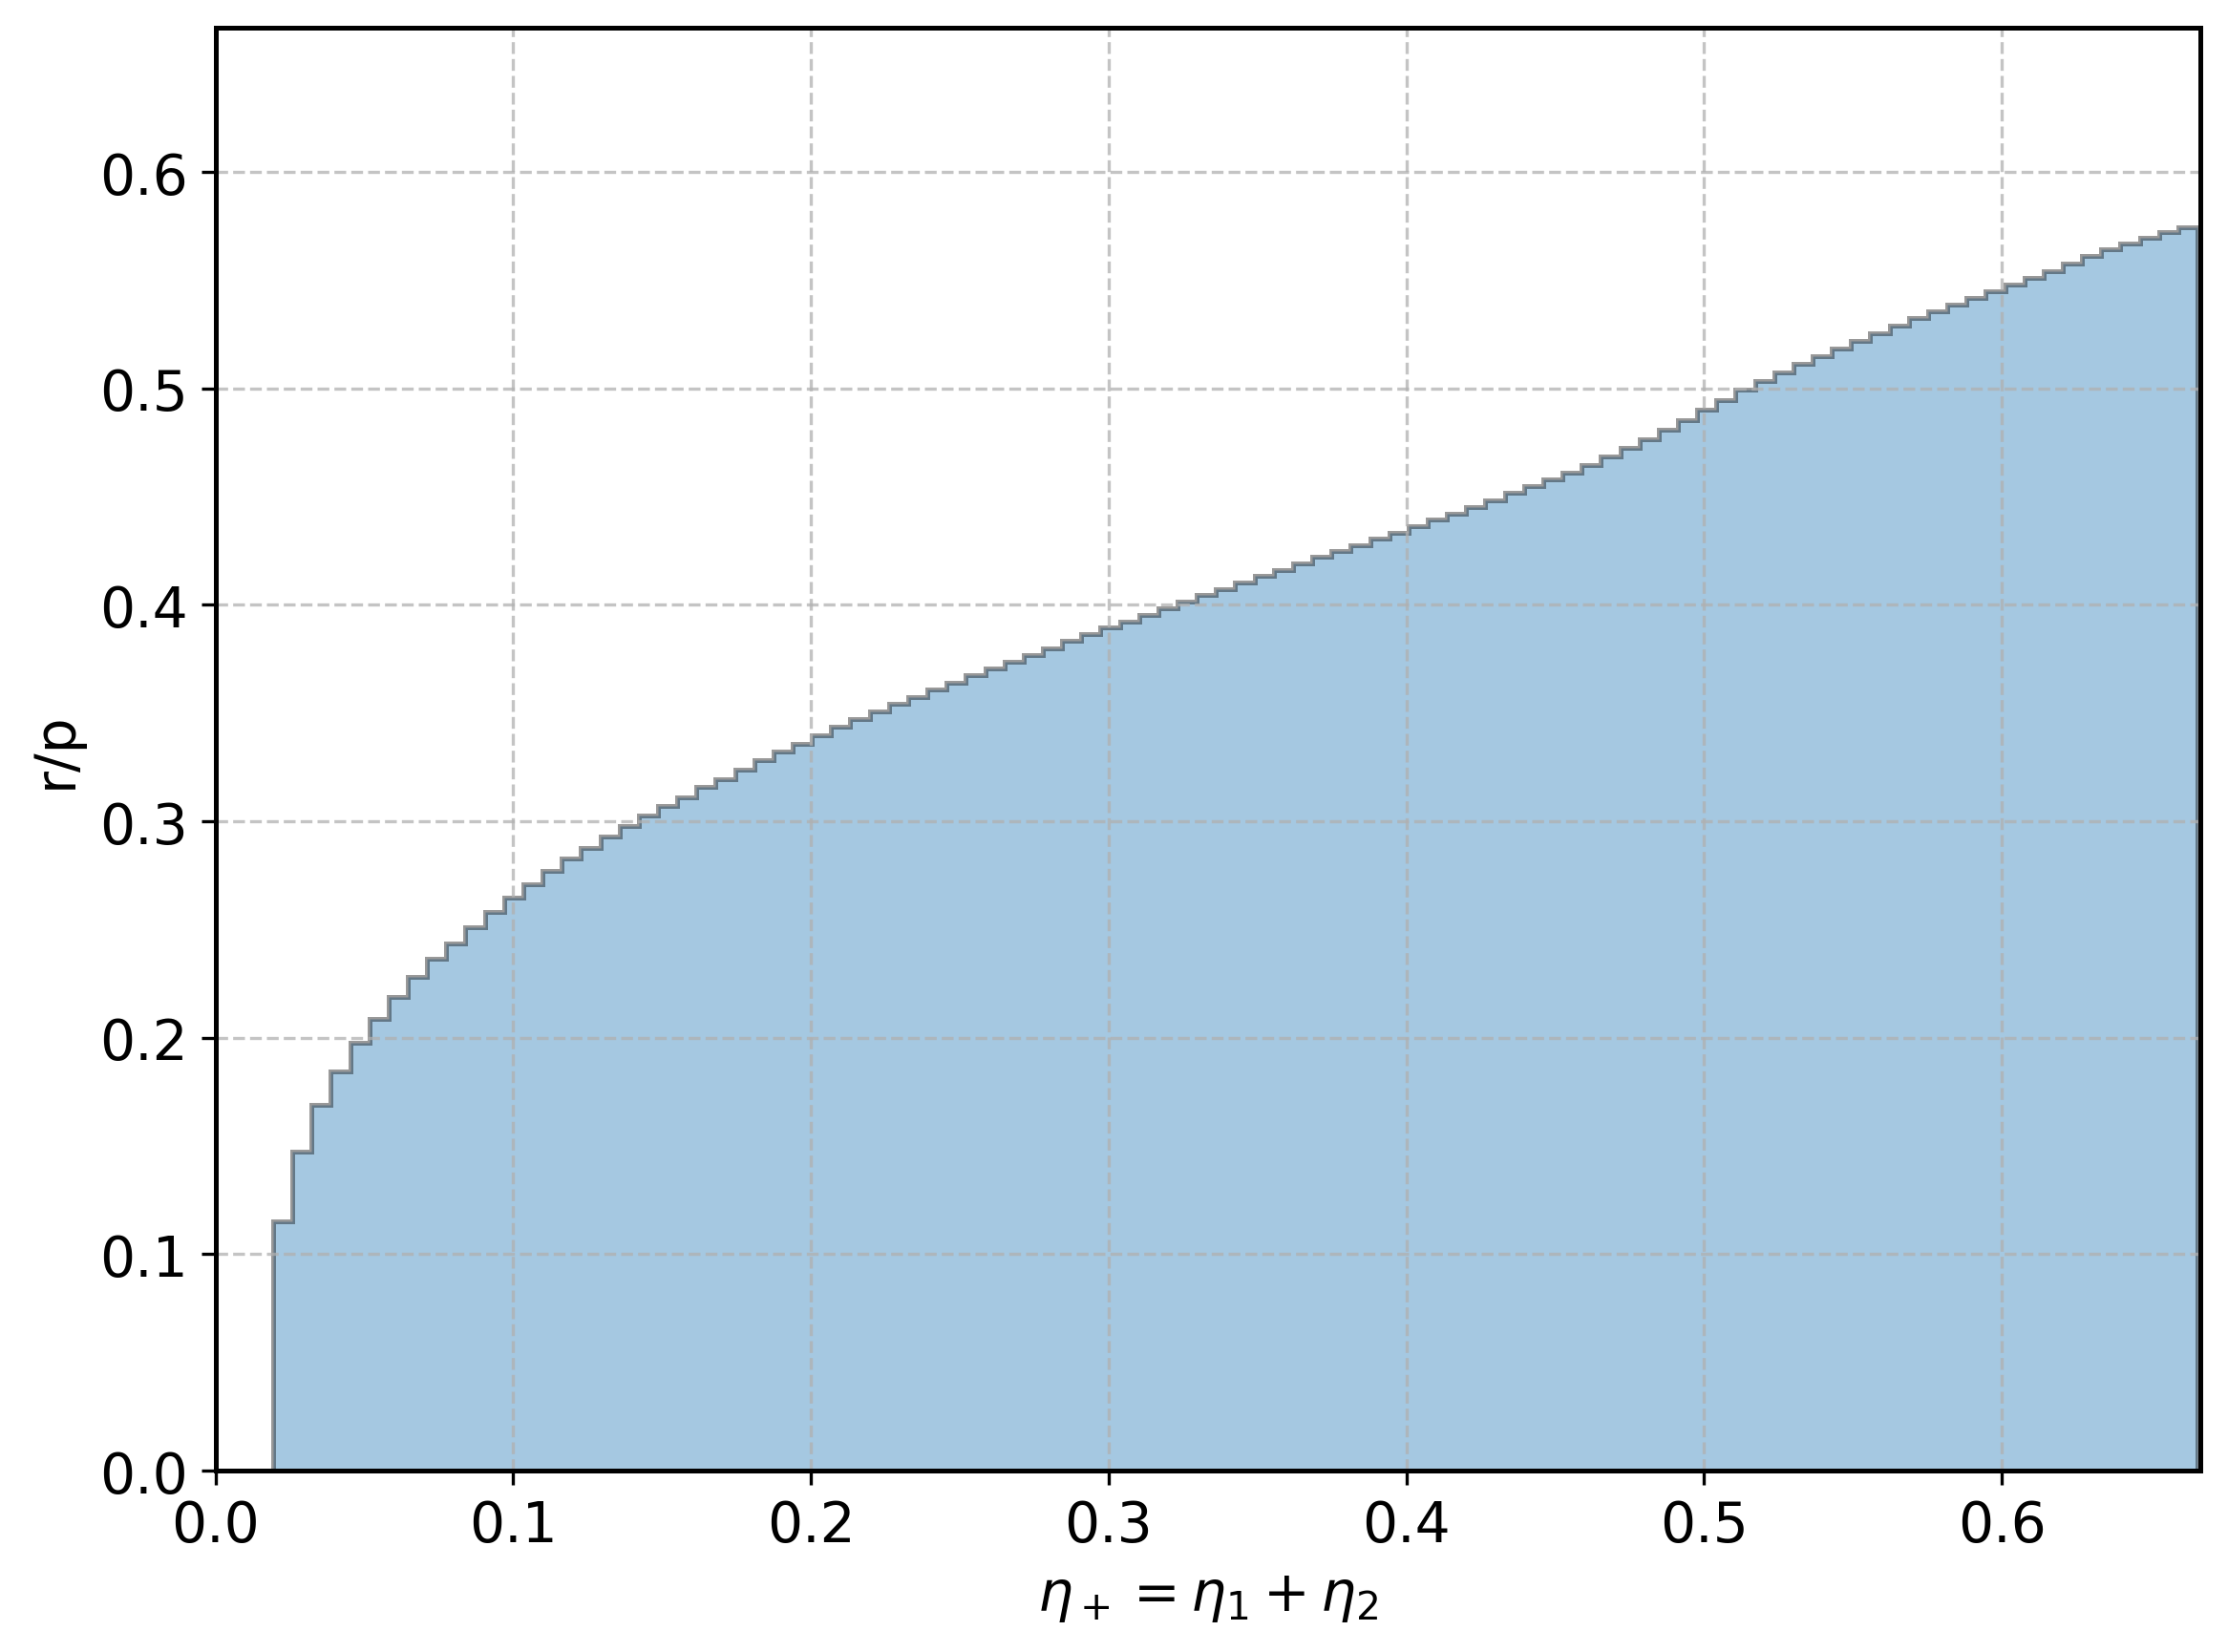
\includegraphics[width=0.49\linewidth]{figures/chapter4/position/eta_3pix_rad_cumulative}
    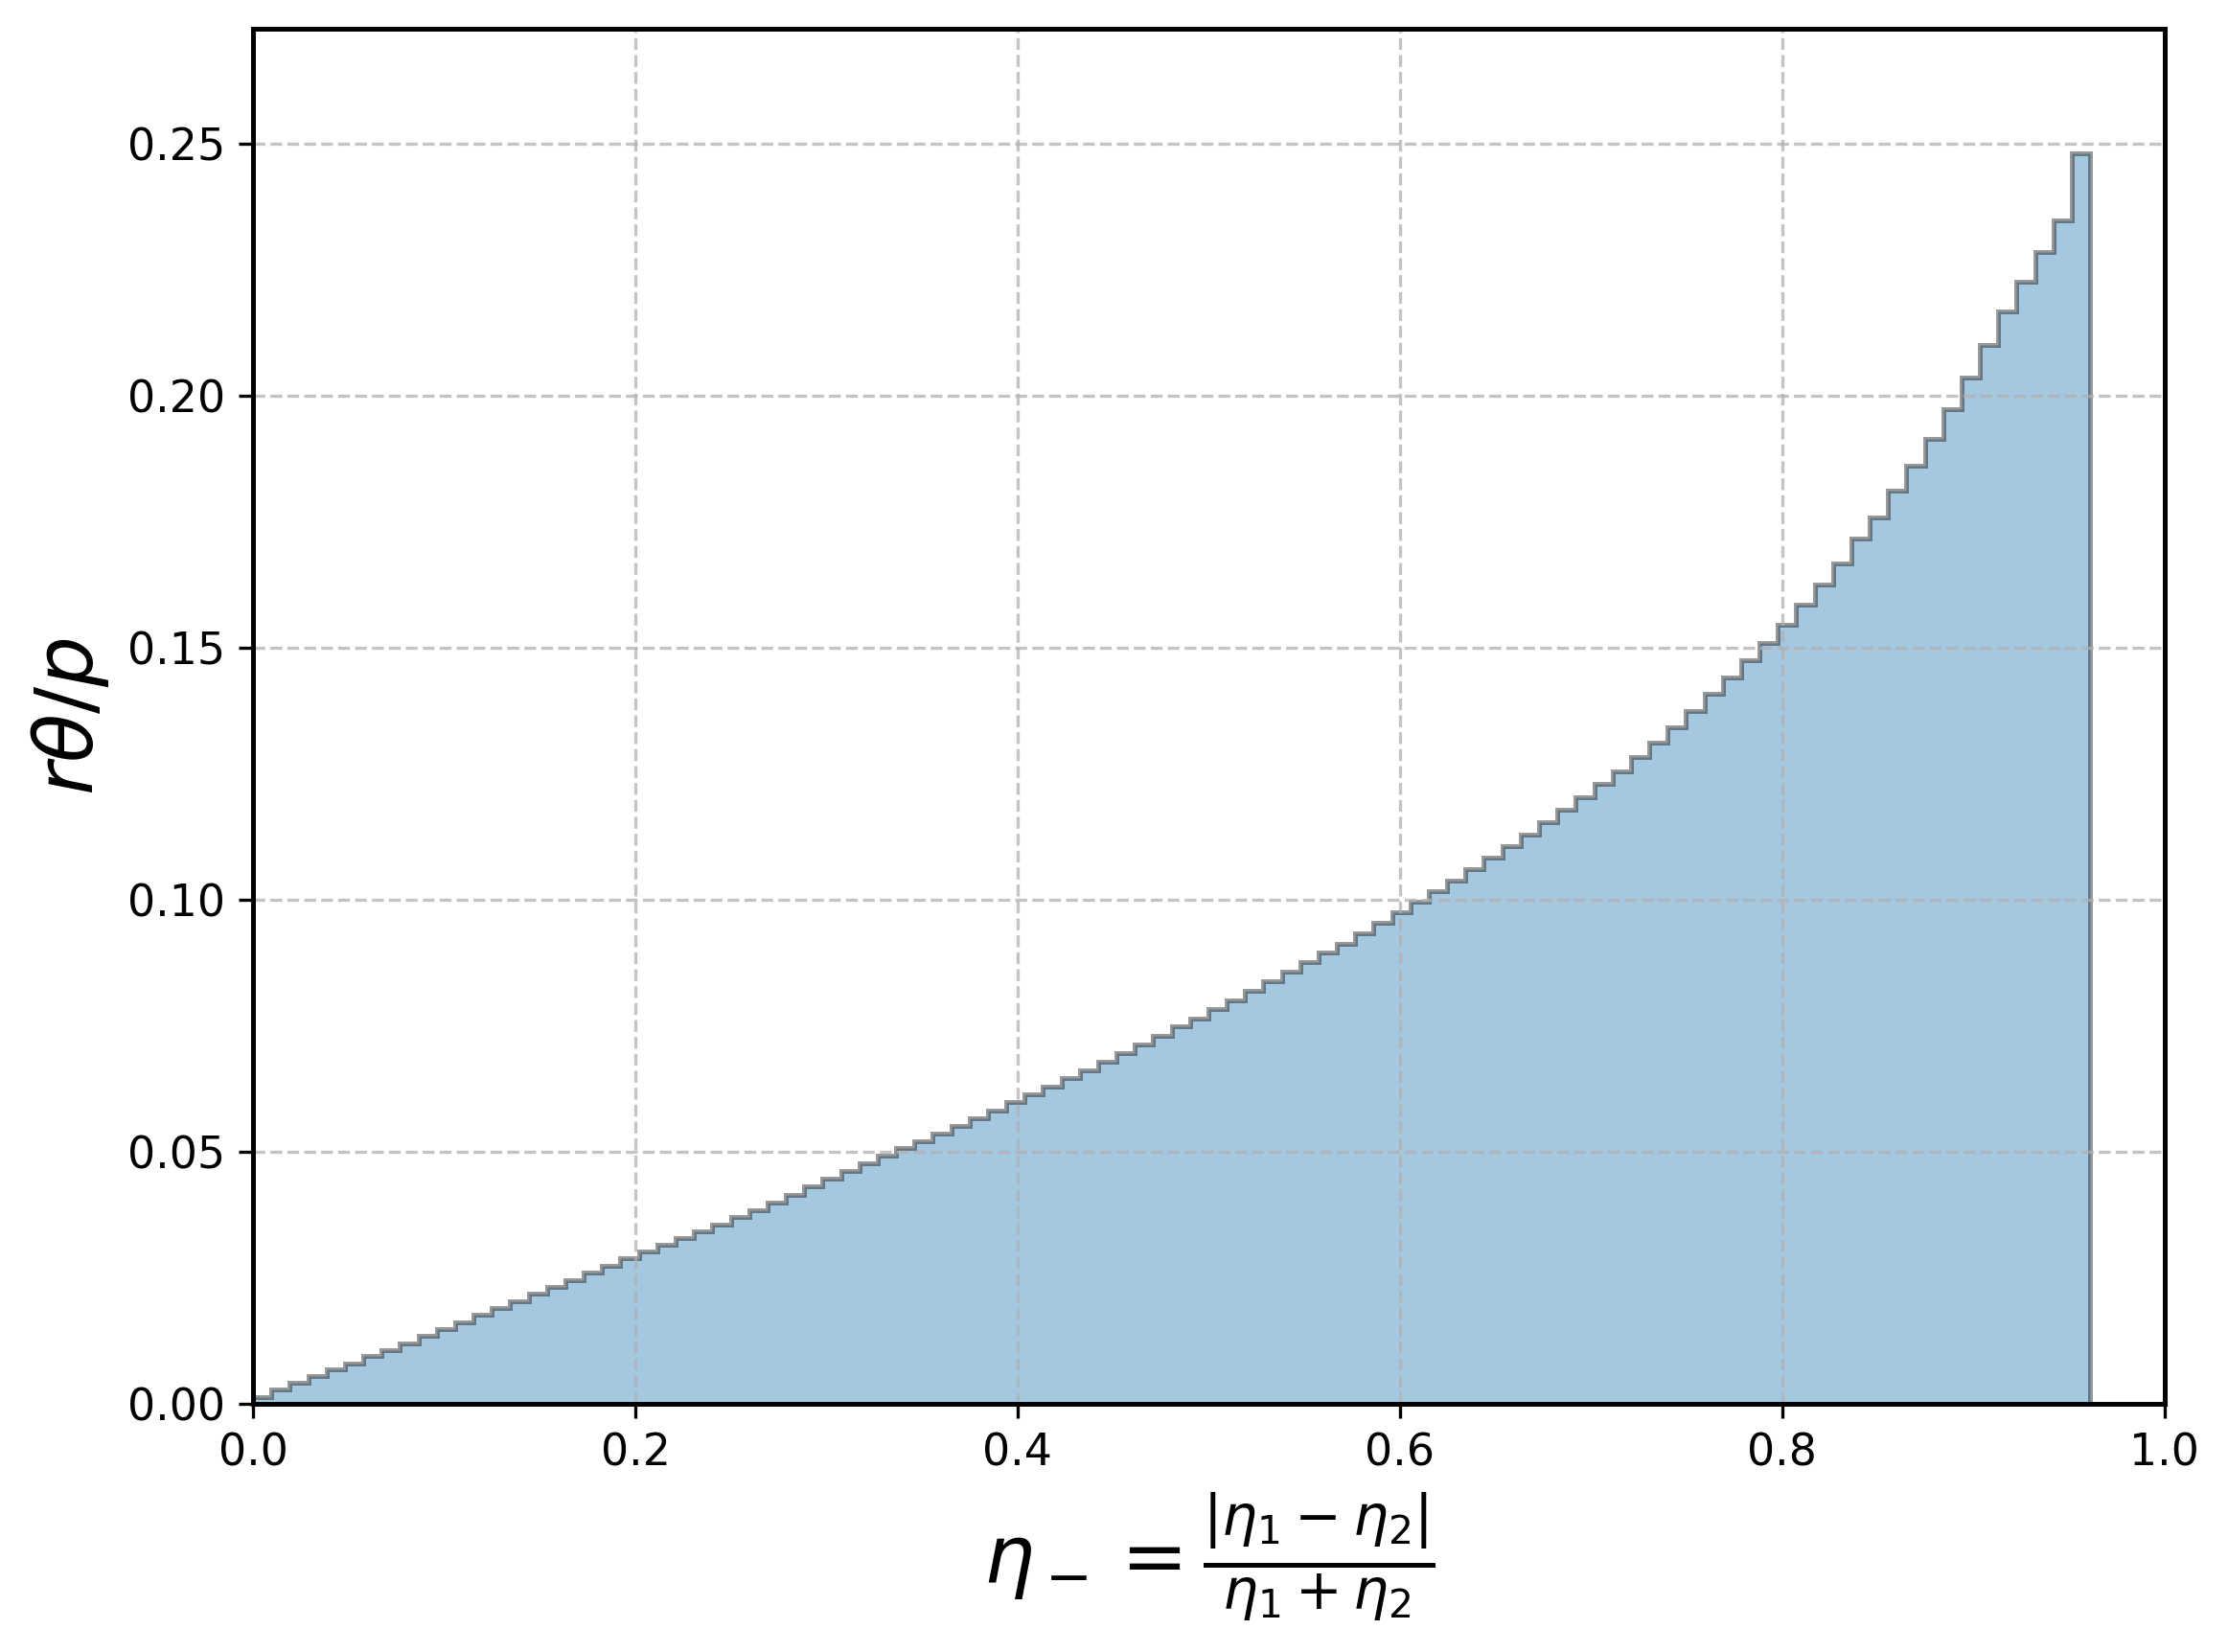
\includegraphics[width=0.49\linewidth]{figures/chapter4/position/eta_3pix_ang_cumulative}
    \caption{Cumulative distributions for $\eta_+$ (left panel) and $\eta_-$ (right panel) variables. }
    \label{fig:eta_3pix}
\end{figure}


For three-pixel events, the non-uniformity of the spatial distribution is primarily a geometrical effect. Even though the events are uniformly spread across the two-dimensional surface of the pixel, the transverse width of the relevant sector significantly varies along the reconstruction axis, reaching a peak after the middle point. This variation directly shapes the projected distribution, which is exactly what is observed in the left panel of Fig. \ref{fig:3pix_scatter}.

\begin{figure}[!b]
    \centering
    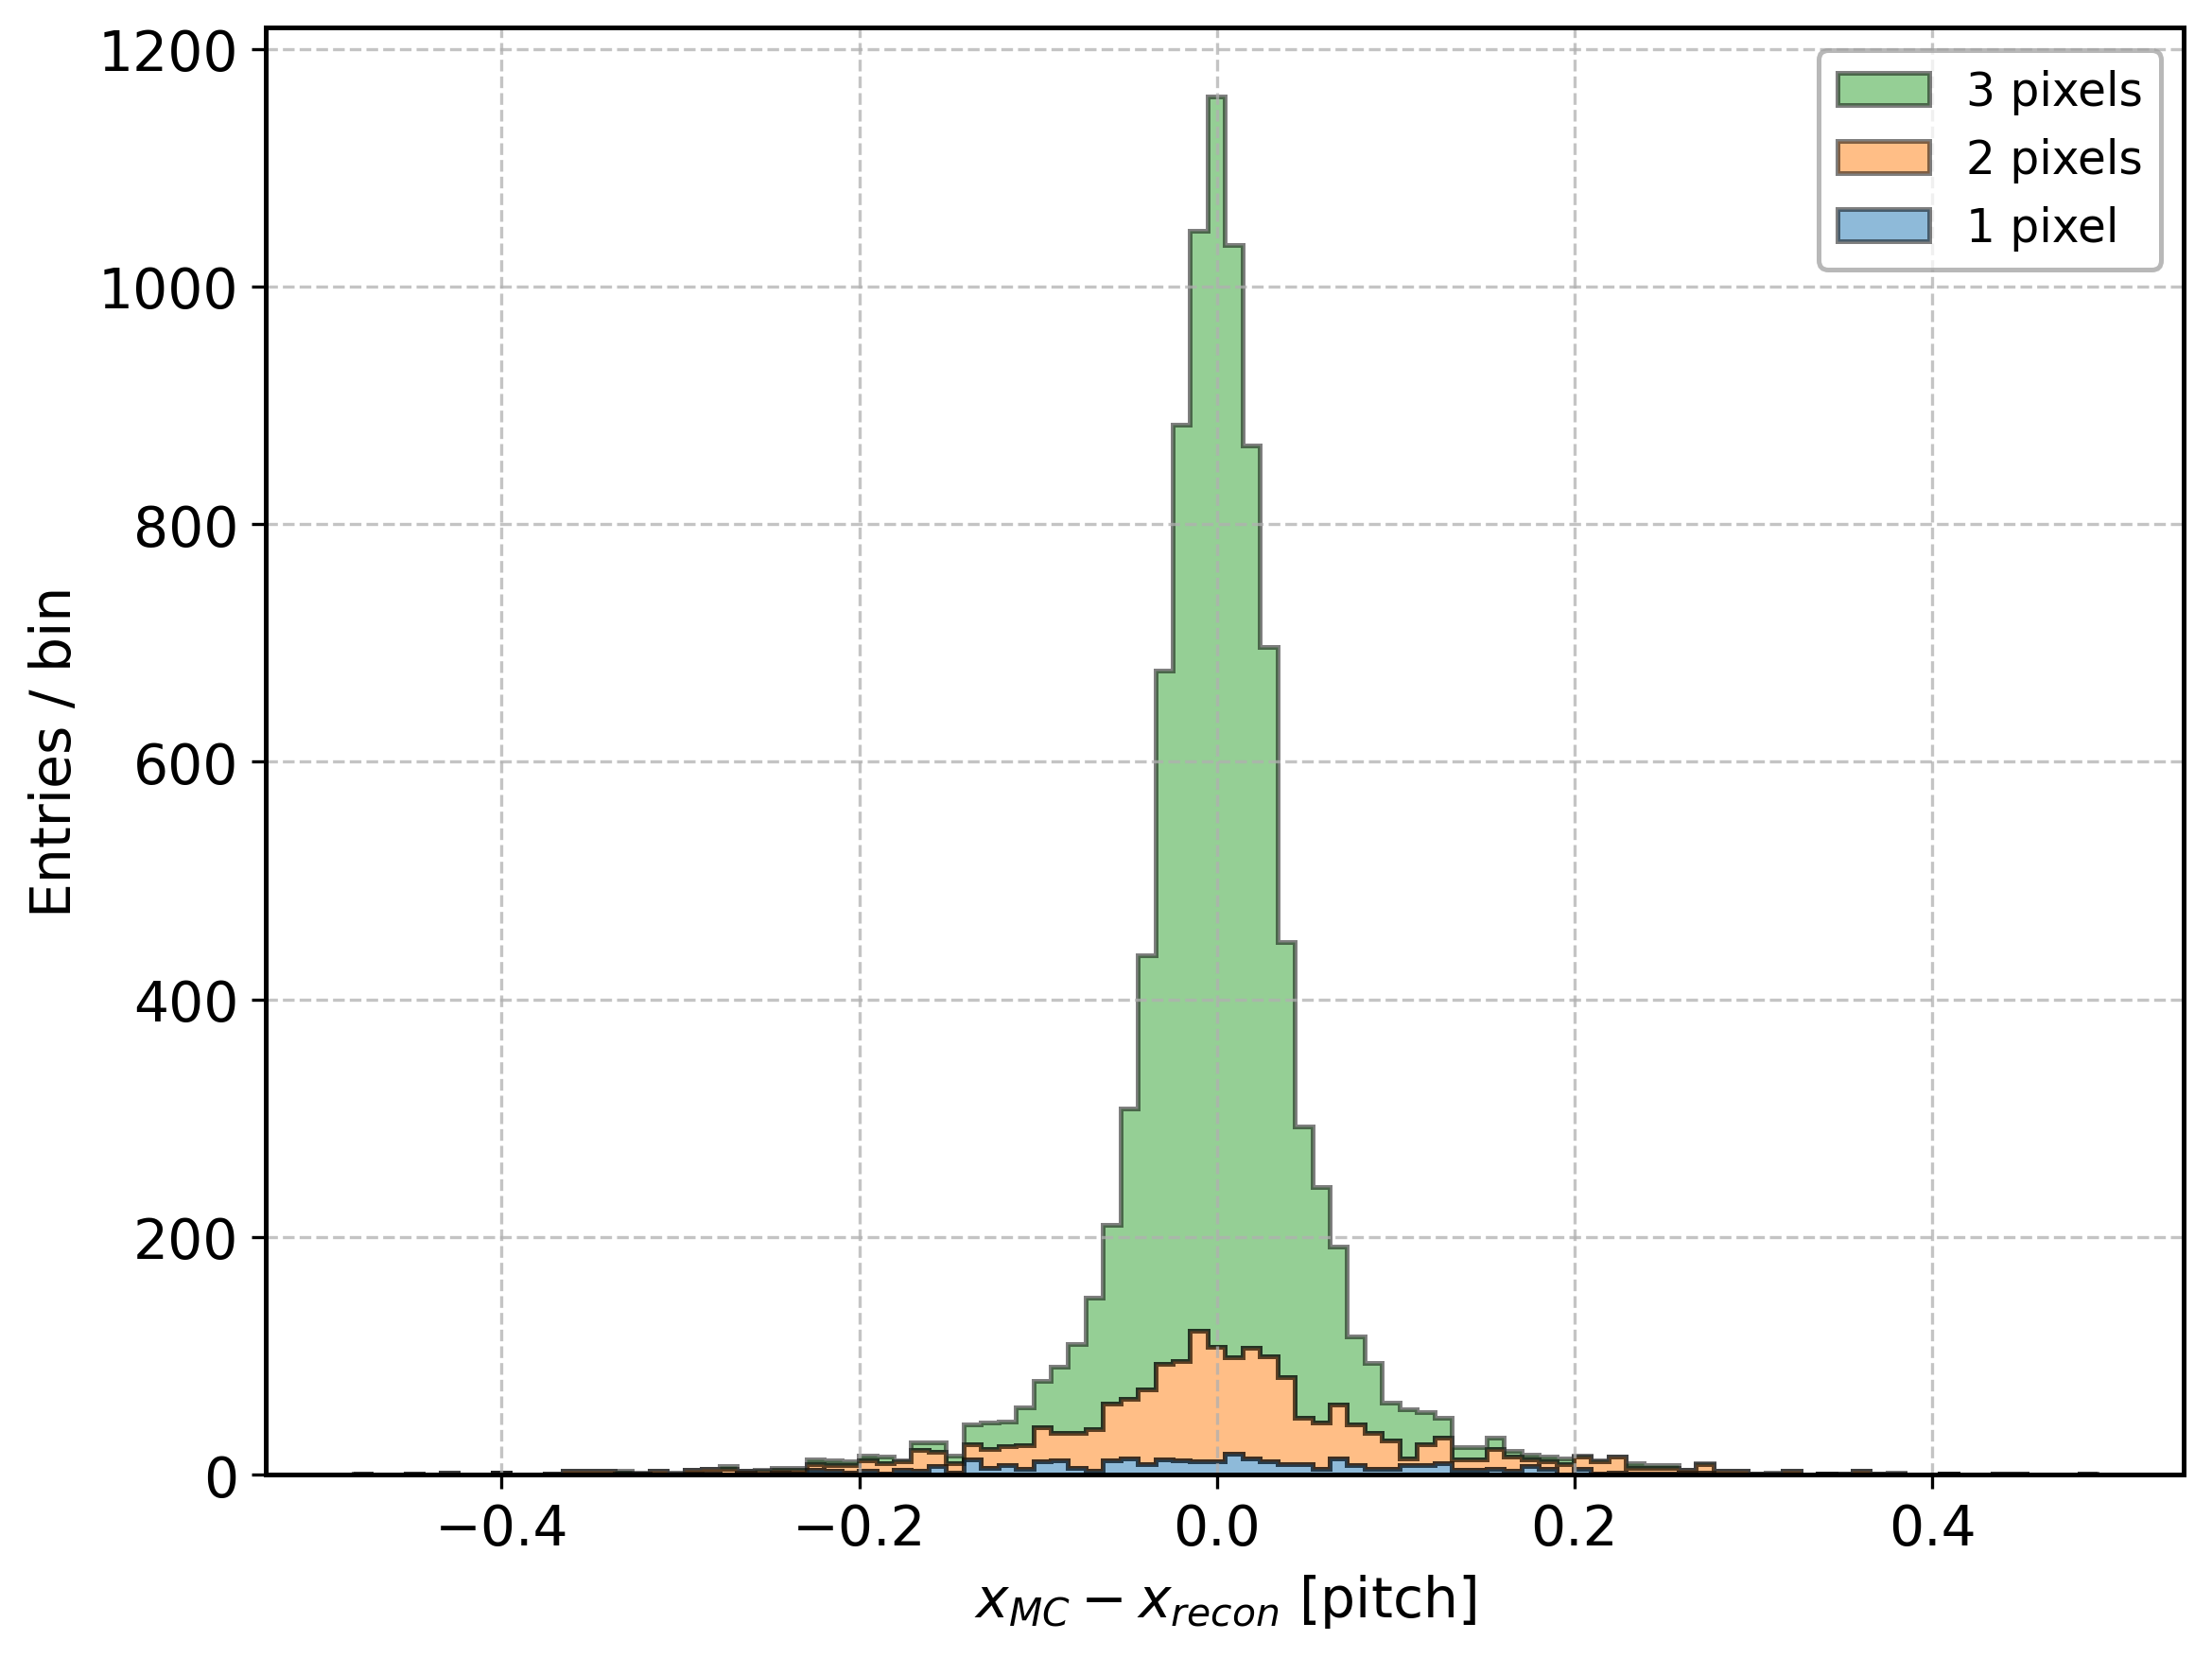
\includegraphics[width=0.49\linewidth]{figures/chapter4/position/eta_unmodeled_dx}
    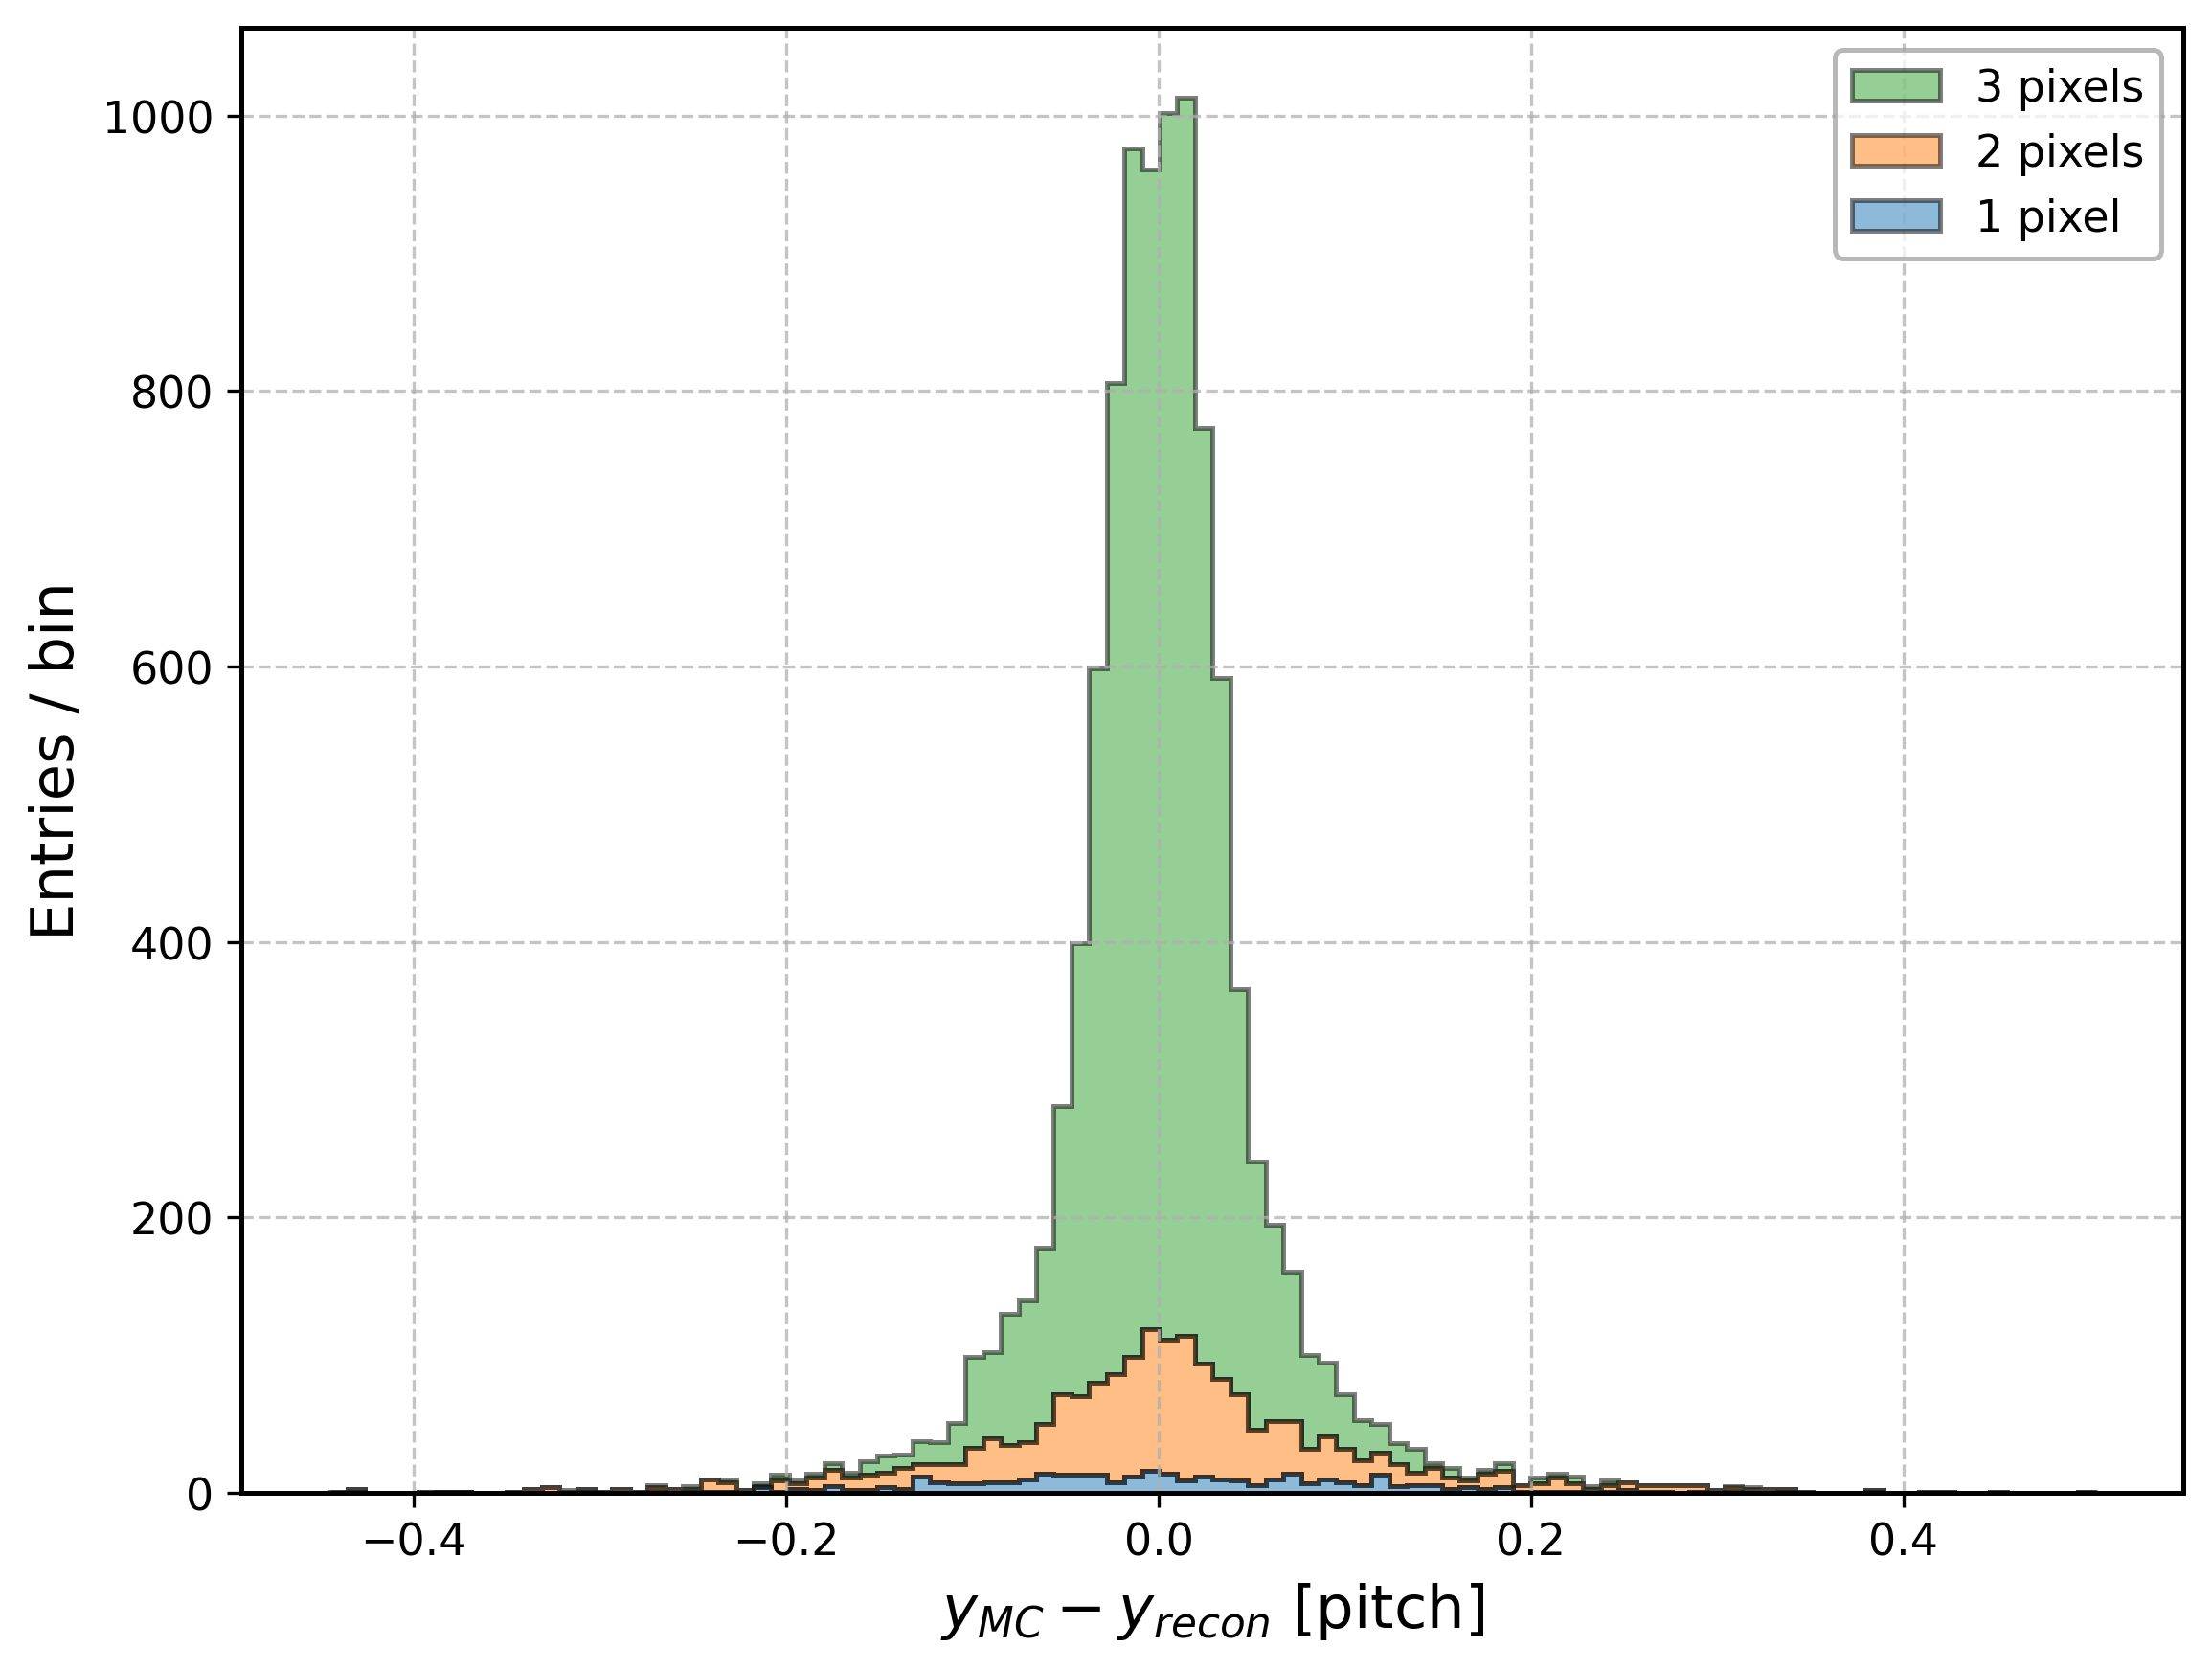
\includegraphics[width=0.49\linewidth]{figures/chapter4/position/eta_unmodeled_dy}
    \caption{Residuals distributions of the eta algorithm for the $x$ and $y$ directions, calculated as the difference between the reconstructed and the Monte Carlo truth $x$ and $y$ components. The events are separated by cluster size, with each color representing a specific cluster size. The histograms are stacked on each other. The simulation is made with a 8 keV monochromatic source, 20 ENC of noise and ratio between the diffused charge cloud sigma and the pitch of 15\%.}
    \label{fig:eta_dx_dy}
\end{figure}

A similar behaviour is observed for $\eta_-$ projecting onto the axis perpendicular to the radial one. These non-uniformities heavily affect the shape of $\eta_+$ and $\eta_-$ distributions. Fig. \ref{fig:3pix_rad_eta} shows a comparison between the $\eta_+$ with and without the correction for uniformity.

After correcting non-uniformities in the $\eta_+$ and $\eta_-$ distributions with the same iterative approach used for two-pixel events, the cumulative distributions can be calculated. The cumulative distributions are shown in Fig. \ref{fig:eta_3pix}.

The $\eta$ algorithm presented for three-pixel events could also be generalized to all cluster sizes. The only necessary thing to do is identifying the symmetry axes of the specific cluster size and then opportunely define two combinations of the $\eta_i$. However, with an increasing number of pixels involved in an event the charge barycenter algorithm becomes better and the improvement of an $\eta$ algorithm could become negligible. For ASIX only events with up to three pixels have been analyzed, as it is designed to not have big cluster sizes.

Similarly to the likelihood reconstruction method, the $\eta$ algorithm requires a calibration before being able to use it. The relevant difference between the two methods is that the $\eta$ algorithm does not need Monte Carlo truth information, but it can be directly calibrated from observed data. The only condition that has to be satisfied is using a source that uniformly illuminates the detector.

After analyzing the same dataset as the previous algorithms, the residuals for this reconstruction method are shown in Fig. \ref{fig:eta_dx_dy}. The residuals distributions are similar to those obtained with the MLE algorithm, but the tails are not as prevalent as for the MLE. This behavior is confirmed by the EEF, shown in Fig. \ref{fig:eta_unmodeled_eef}. 
%Tab. \ref{tab:eef_eta_unmodeled} shows the distances at which the EEF contains 50\% and 90\% of the events.


\begin{figure}[!b]
    \centering
    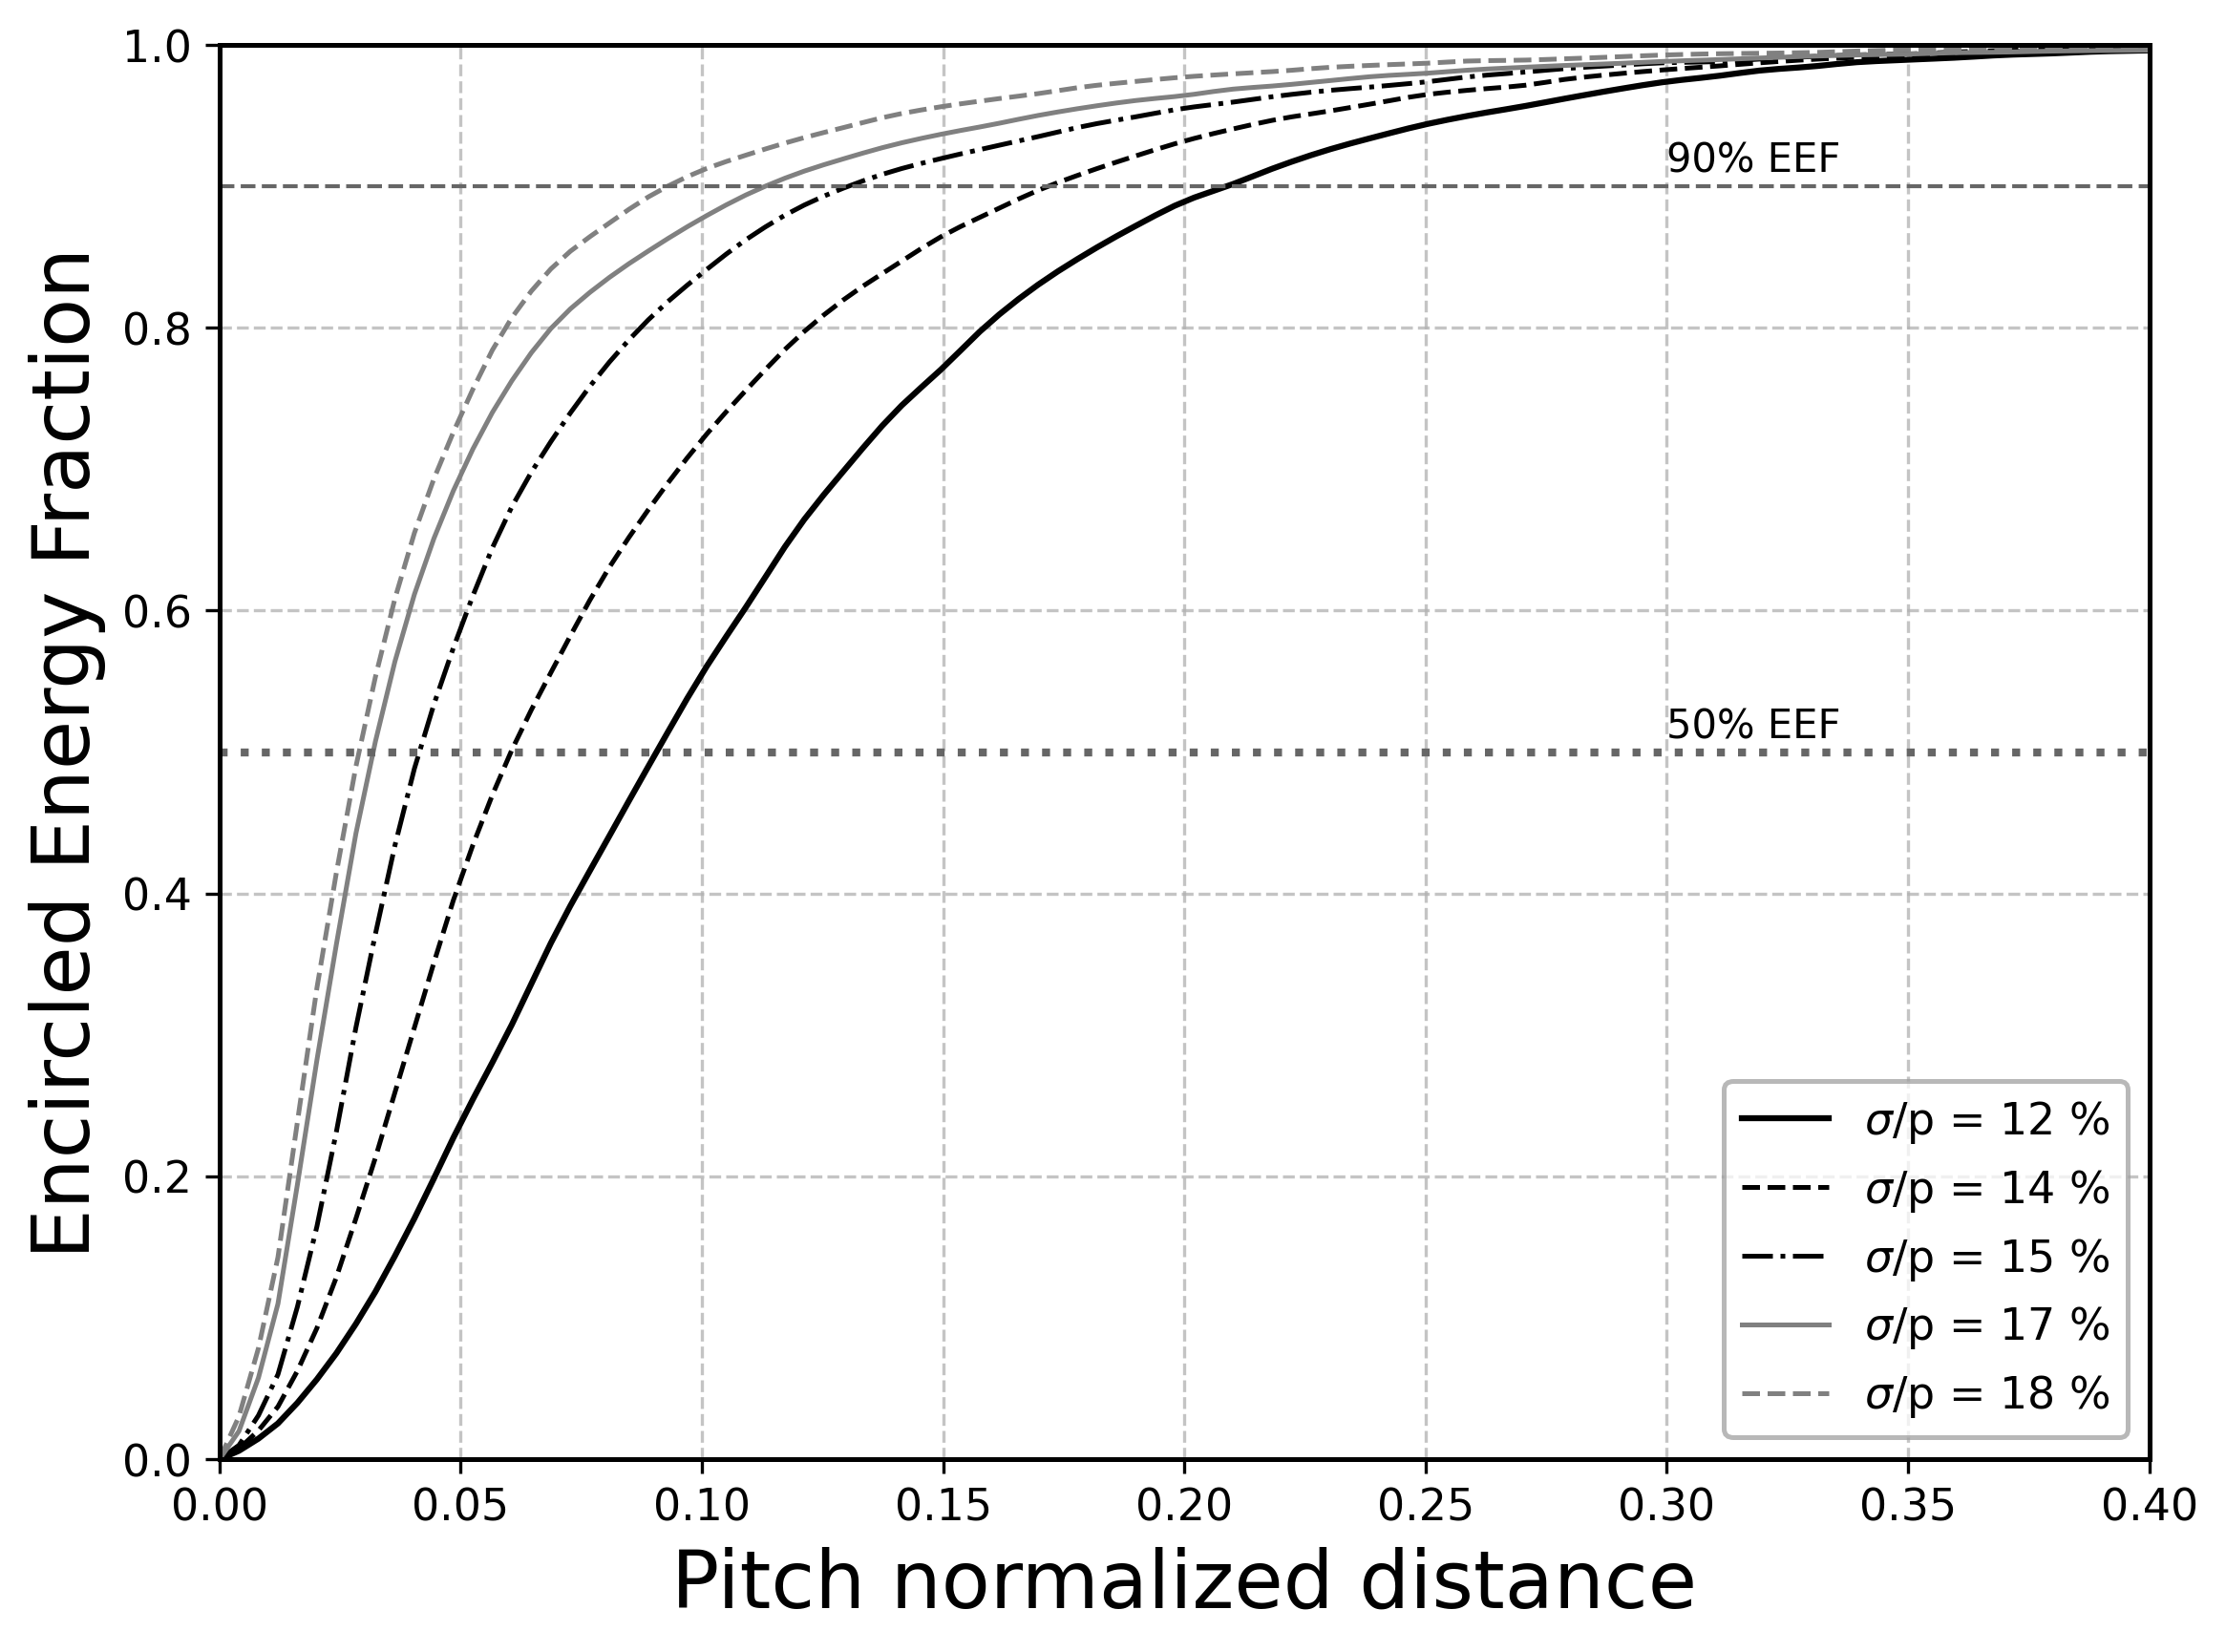
\includegraphics[width=0.7\linewidth]{figures/chapter4/position/eta_unmodeled_eef}
    \caption{Encircled energy fraction of the $\eta$ reconstruction algorithm for different values of the ratio between the diffused charge cloud and the pixel pitch as a function of the pitch normalized distance. The simulation is made with 20 ENC of noise.}
    \label{fig:eta_unmodeled_eef}
\end{figure}

%\begin{table}[htbp]
%\centering
%\begin{tabular}{c cccc}
%$\langle \sigma \rangle / p$ & EEF@50\% [pitch] & EEF@90\% [pitch]\\
%\midrule
%12.2 & 0.09 & 0.21 \\
%13.7 & 0.06 & 0.17 \\
%15.2 & 0.04 & 0.13 \\
%16.8 & 0.03 & 0.11 \\
%18.3 & 0.03 & 0.09 \\
%\bottomrule
%\end{tabular}
%\caption{Pitch distances at which EEF contains 50\% and 90\% of the events with the $\eta$ algorithm reconstruction, as a function of the ratio $\langle \sigma \rangle / p$. The values are extracted from Fig. \ref{fig:eta_unmodeled_eef}}
%\label{tab:eef_eta_unmodeled}
%\end{table}

The strength of this method is that a Monte Carlo simulation is not necessary. However, in case it is available, a different formulation of the $\eta$ algorithm can be made using the true incident positions.  In this case it is required knowing the charge diffusion model, but contrary to the likelihood method there are some approximations that can be made, making possible to solve analytically the problem. 

In the case of two-pixel events the position can only be reconstructed along the line connecting the two pixel centers, thus it is one-dimensional problem, as already seen above. Considering a photon which impacts on this line, the charge diffusion can be modeled as a one-dimensional Gaussian distribution centered on the incident point at a distance $r$ from the central pixel.

Given that the charge cloud dimension is small with respect to the pixel, all the charge is collected by these two pixels. As a consequence, the fraction of charge $\eta$ collected by the outer pixel, defined in Eq. \ref{eq:eta_2pix}, is a function of $r$ and can be calculated as the integral of the Gaussian

\begin{equation}
\eta(r) = \int ^{\infty}_{p/2} \frac{1}{\sqrt{2\pi}\sigma} \exp \left[ - \frac{(r' - r)^2}{2\sigma^2}  \right] dr' = \Phi \left( \frac{r - p/2}{\sigma} \right),
\label{eq:eta_2pix_int}
\end{equation}
where $\Phi(z)$ is the cumulative density function of the standard normal distribution and $p$ is the pixel pitch. Eq. \ref{eq:eta_2pix_int} can be inverted to find

\begin{equation}
r(\eta) = \frac{p}{2} + \sigma \Phi^{-1}(\eta),
\label{eq:eta_2pix_final}
\end{equation}
where $\Phi^{-1}(p)$ is the percent point function of the standard normal distribution.

The only unknown parameter in Eq. \ref{eq:eta_2pix_final} is $\sigma$, that could be estimated with Eq. \ref{eq:diff_sigma_dist}. However, this estimate would not take into account the presence of events occuring far from the axis, as shown in Fig. \ref{fig:2pix_scatter}. For this reason Monte Carlo simulations can be used to estimate the parameter.

To estimate $\sigma$ the projected distance $r$ of the Monte Carlo truth position onto the axis connecting the two pixel centers is calculated. A two-dimensional histogram is calculated using the resulting projected distance and $\eta$, as shown in Fig. \ref{fig:eta_2pix_r_distr}.

\begin{figure}[!b]
    \centering
    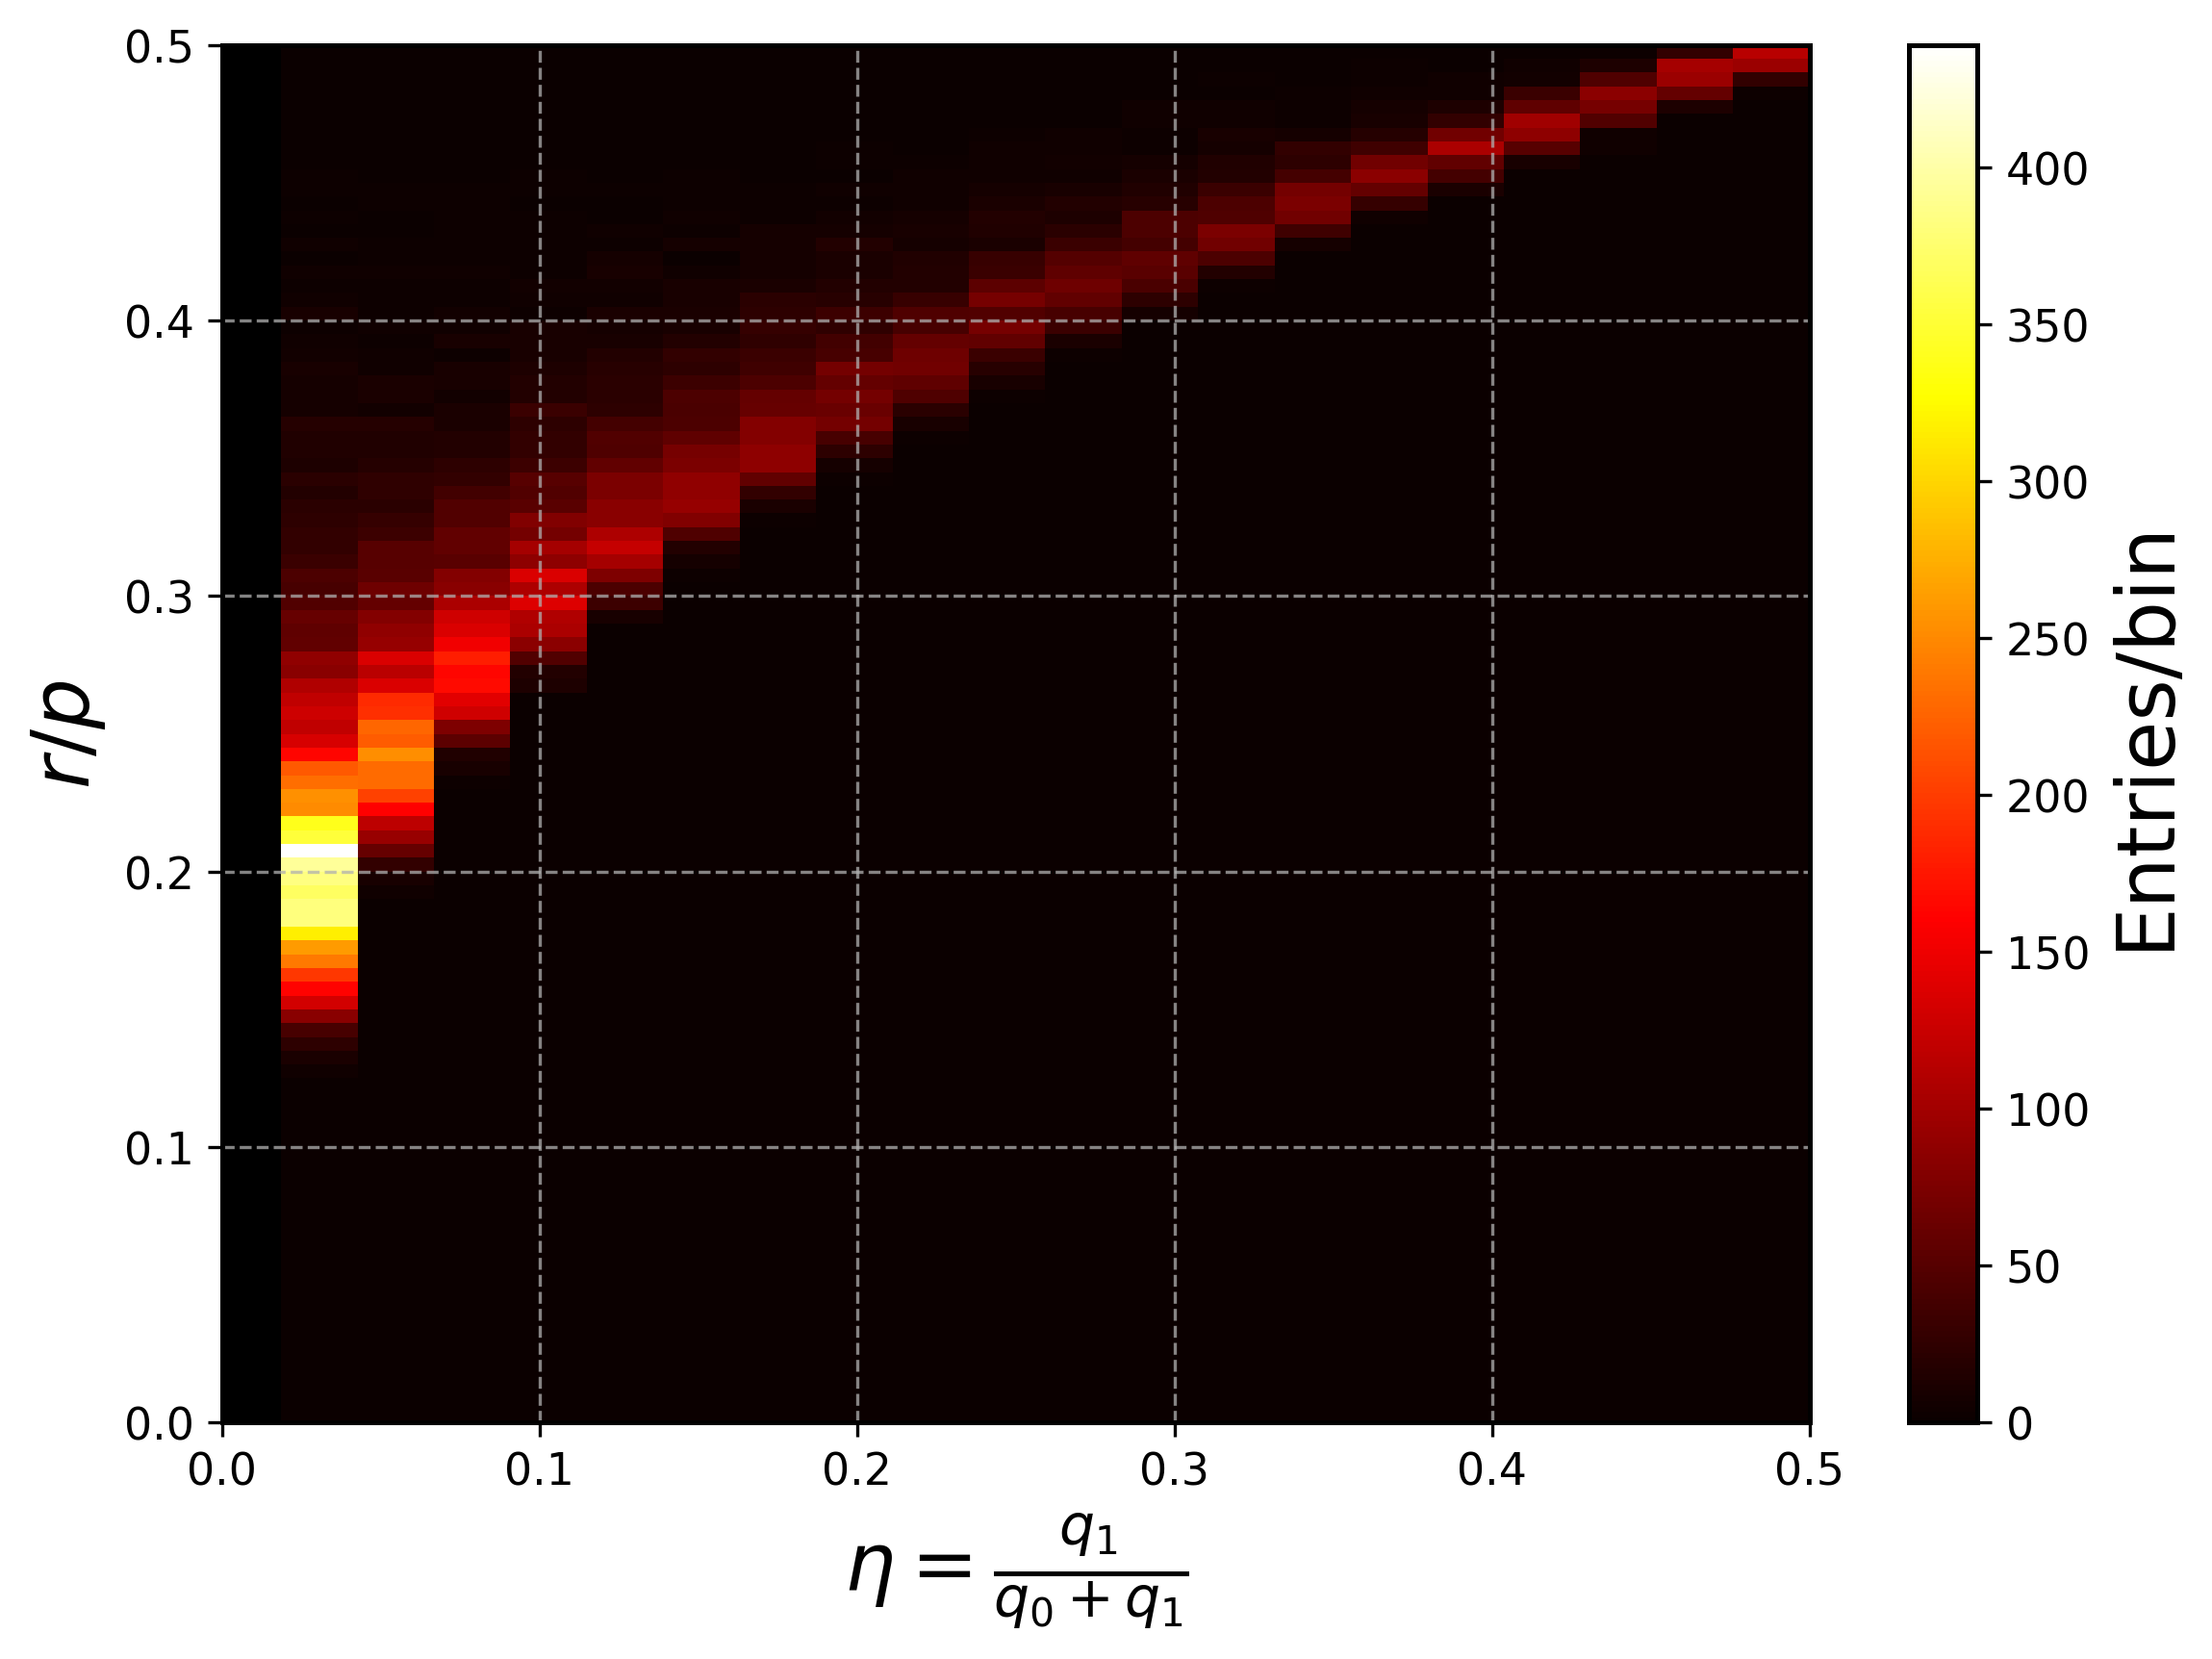
\includegraphics[width=0.49\linewidth]{figures/chapter4/position/eta_2pix_hist}
    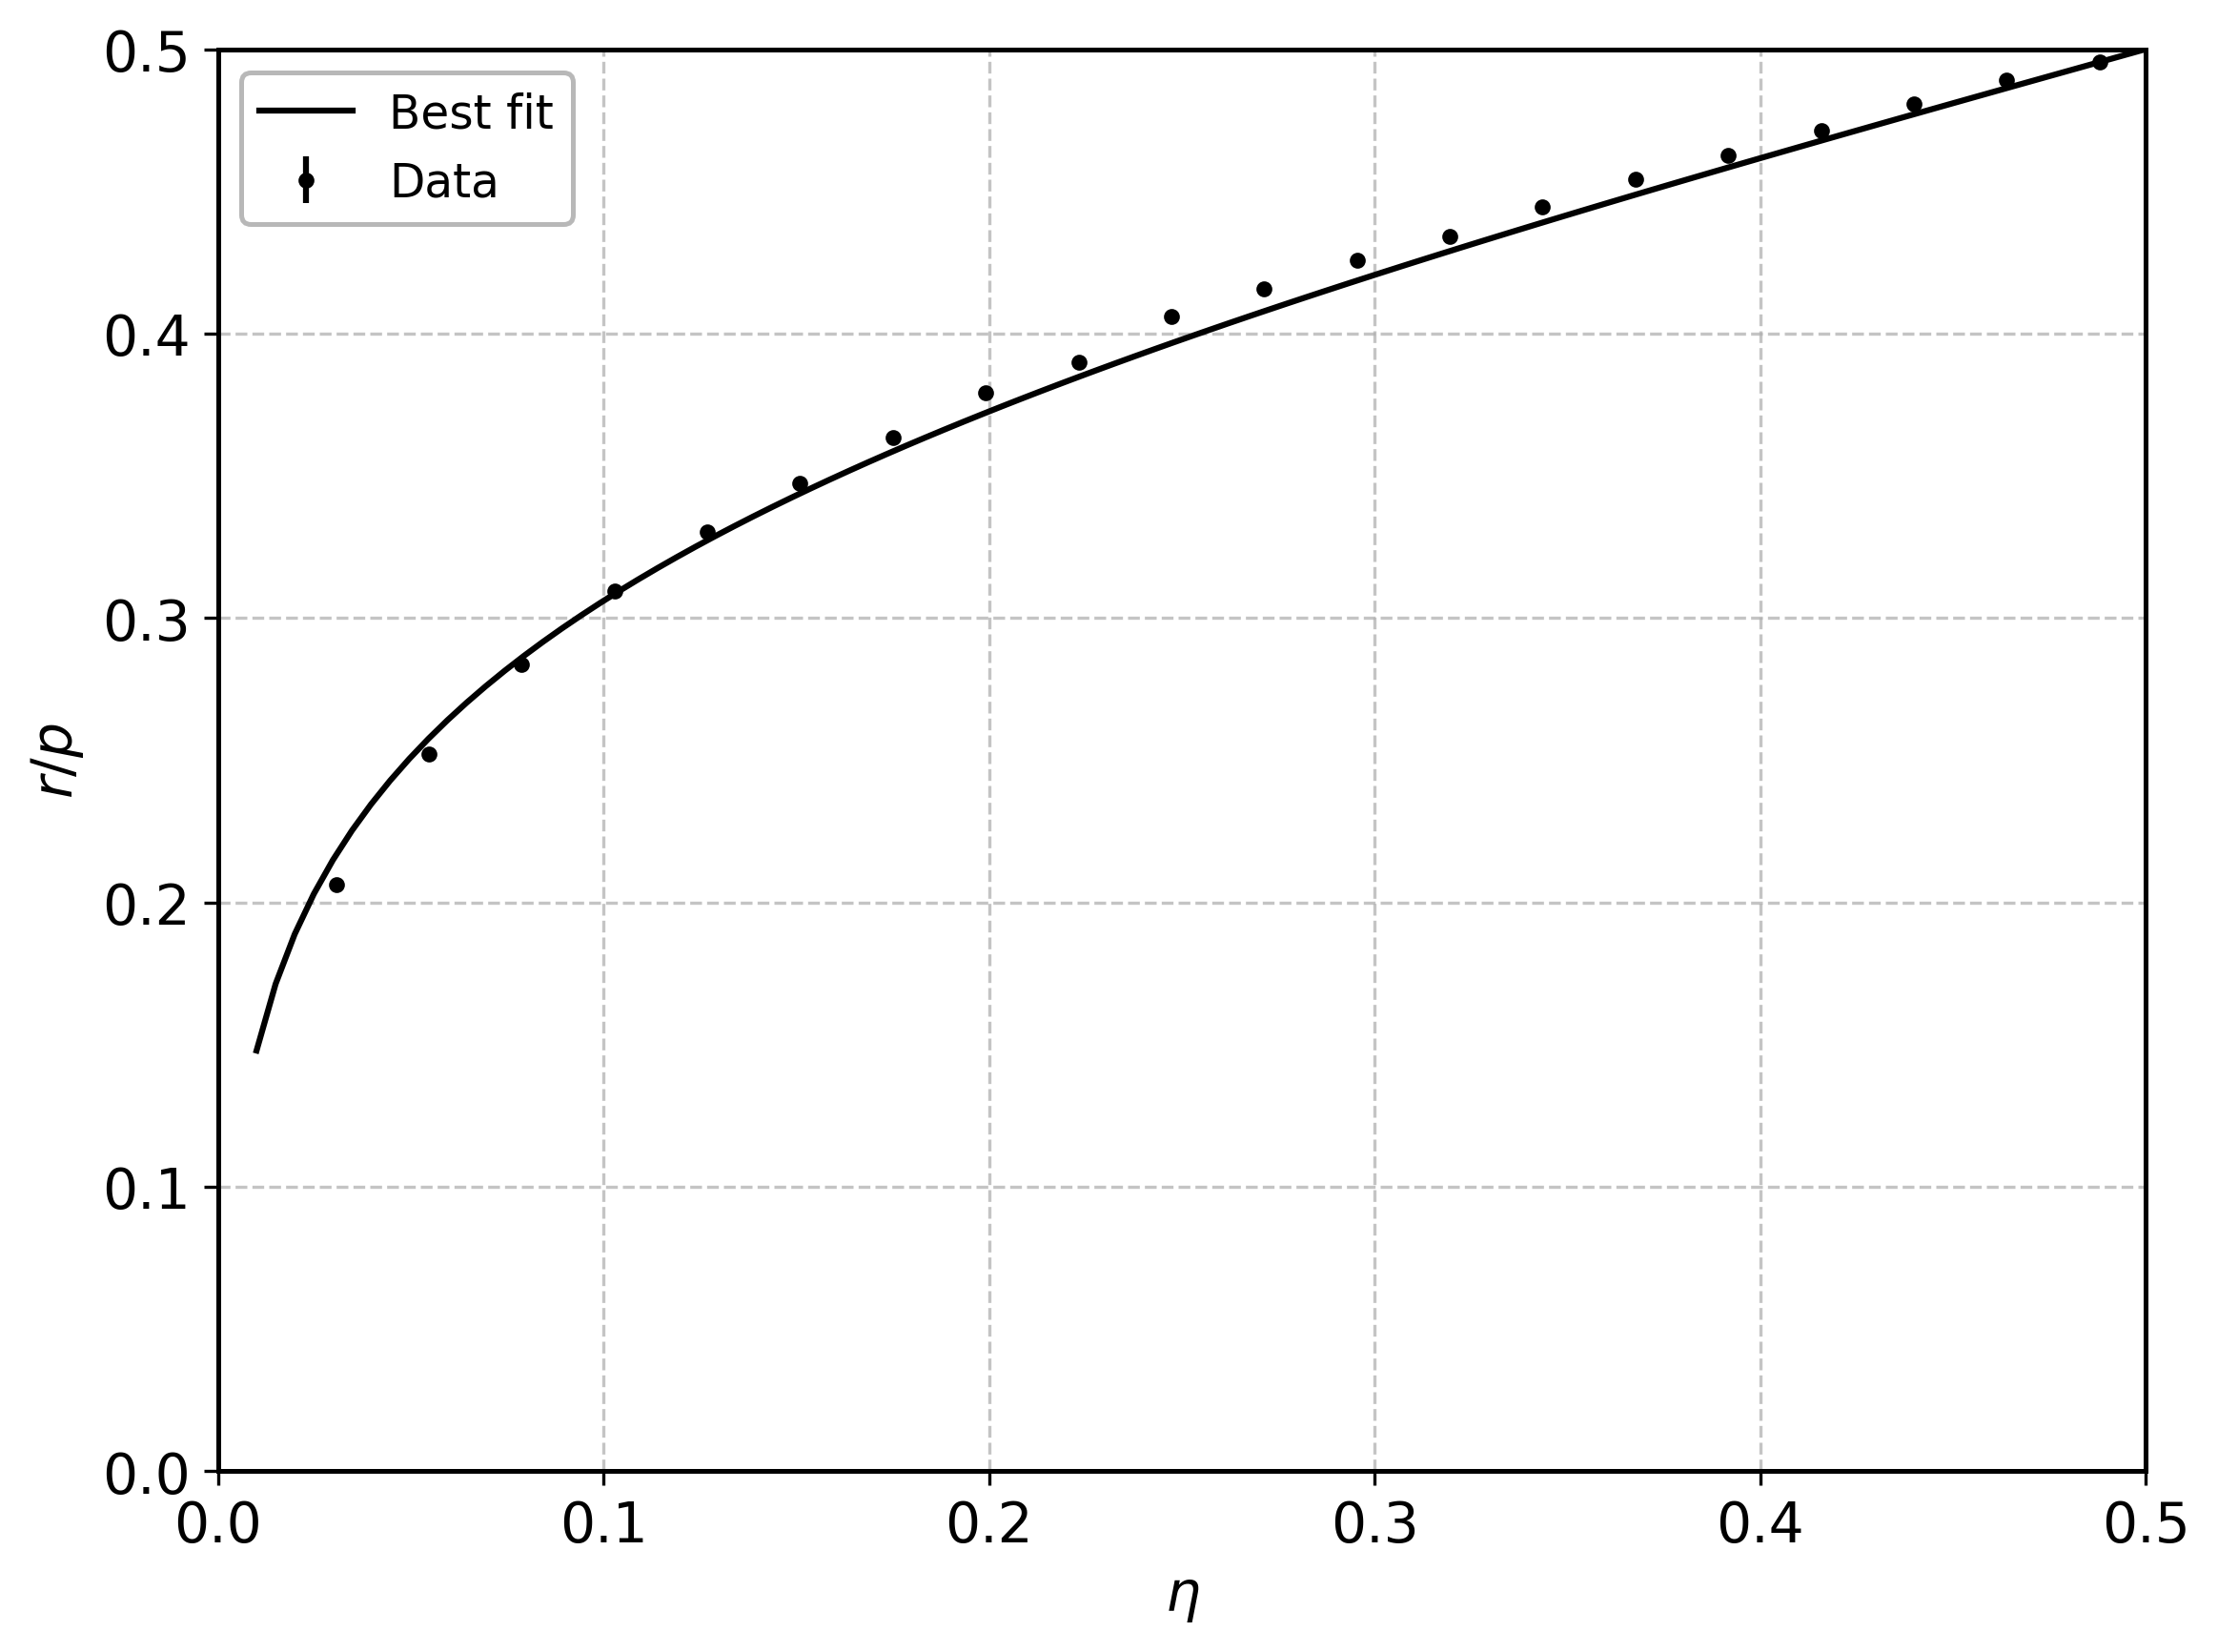
\includegraphics[width=0.49\linewidth]{figures/chapter4/position/eta_2pix_fit}
    \caption{Two-dimensional histogram showing the distribution of $r$ as a function of $\eta$ (left panel) and profile calculated from the latter, using the median of the $r$ distributions for each $\eta$ (right panel). The profile is fitted using Eq. \ref{eq:eta_2pix_final} as fit model to find the best-fit value of $\sigma$. The simulation has an estimated $\langle \sigma \rangle / p = 0.15$.}
    \label{fig:eta_2pix_r_distr}
\end{figure}

A profile of this histogram is then obtained by calculating the median of the $r$ distribution for each $\eta$ bins. The choice to use the median has been made because these distributions have long tails, thus the mean would not be the ideal location estimator.

The resulting profile is fitted using Eq. \ref{eq:eta_2pix_final} as fit model, with $\sigma$ being the only free parameter. The profile and the corresponding fit are shown in Fig. \ref{fig:eta_2pix_r_distr}.

A similar approach can be used for three-pixels events. As already said above, this case requires to separate between the radial and the angular coordinates into two independent one-dimensional two-pixel problems.

The idea behind this model is the same already discussed for the unmodeled $\eta$ algorithm. The radial component can be described by the $\eta_+$ variable, considering the two outer pixels as a single one with total charge given by the sum of the two. The problem is reduced to the same of two-pixel events, with the only difference being in the lower integration limit, which now is the distance of the vertex from the center. $\eta_+$ is given by

\begin{equation}
\eta_+(r) = \int ^{\infty}_{p/\sqrt{3}} \frac{1}{\sqrt{2\pi}\sigma} \exp \left[ - \frac{(r' - r)^2}{2\sigma^2}  \right] dr' = \Phi \left( \frac{r - p/\sqrt{3}}{\sigma} \right),
\label{eq:eta_3pix_int}
\end{equation}
which leads to

\begin{equation}
r(\eta_+) = \frac{p}{\sqrt{3}} + \sigma \Phi^{-1}(\eta_+).
\label{eq:eta_3pix_no_final}
\end{equation}

\begin{figure}[!b]
    \centering
    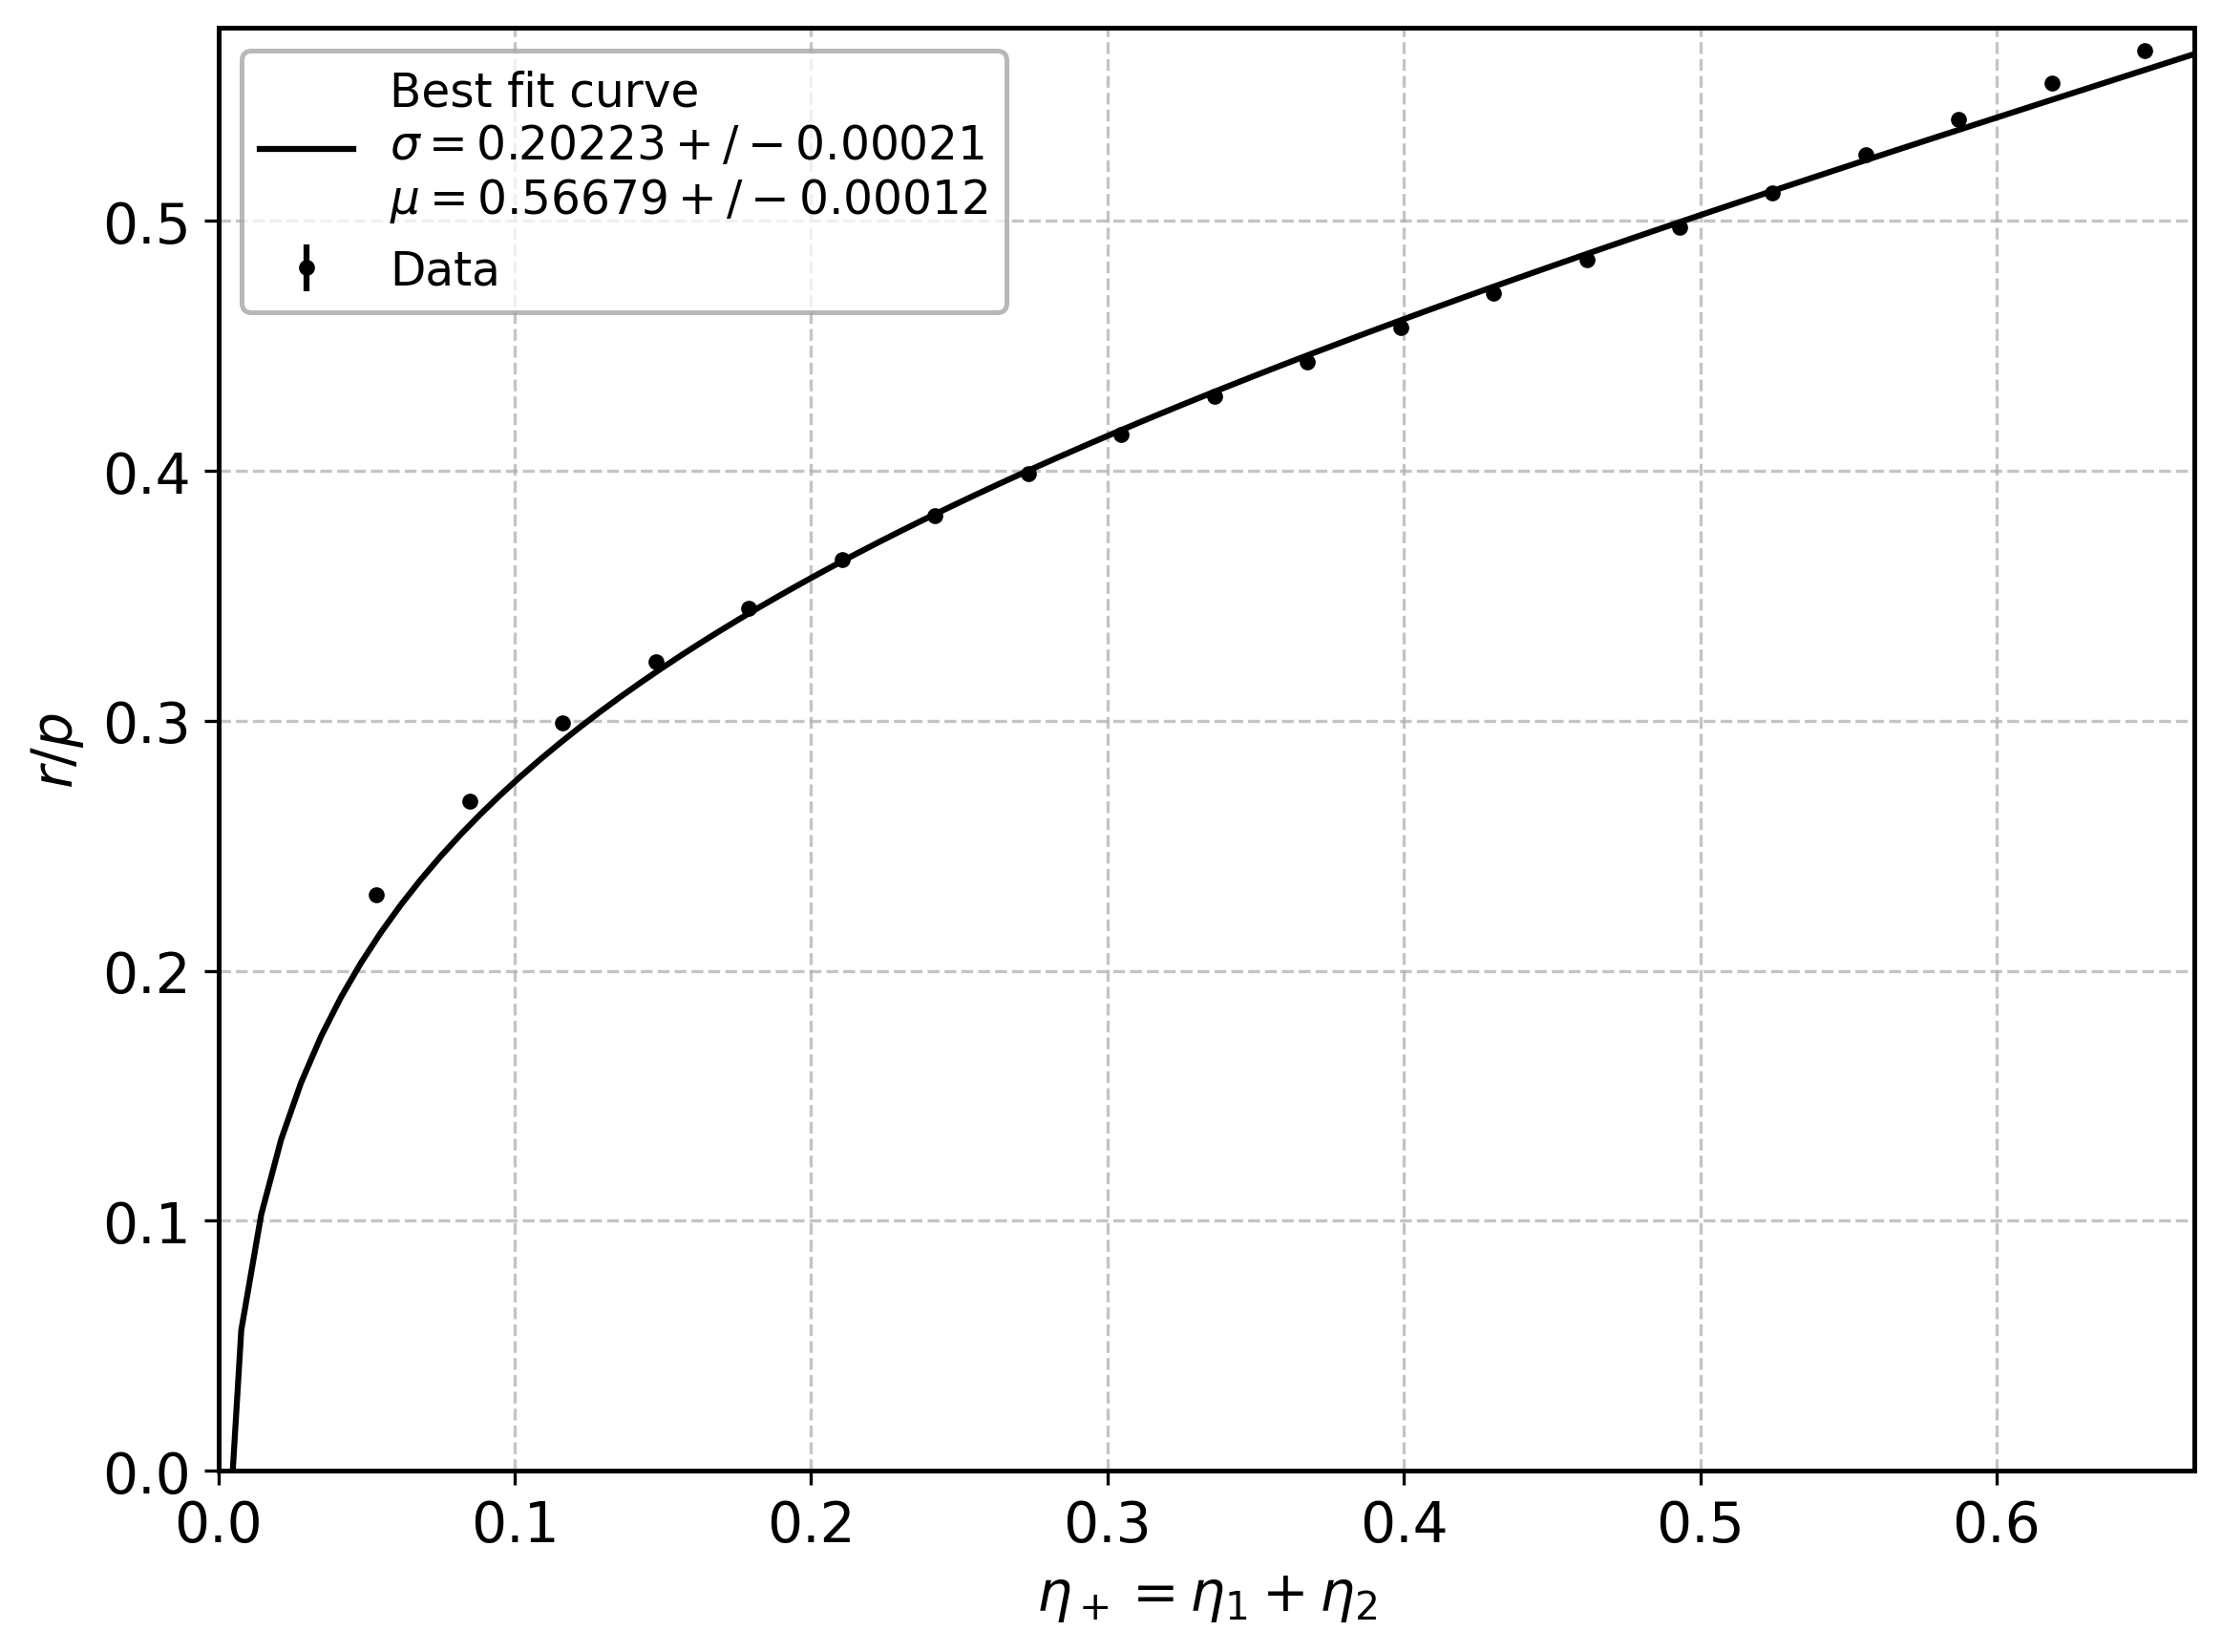
\includegraphics[width=0.49\linewidth]{figures/chapter4/position/eta_3pix_radial_fit}
    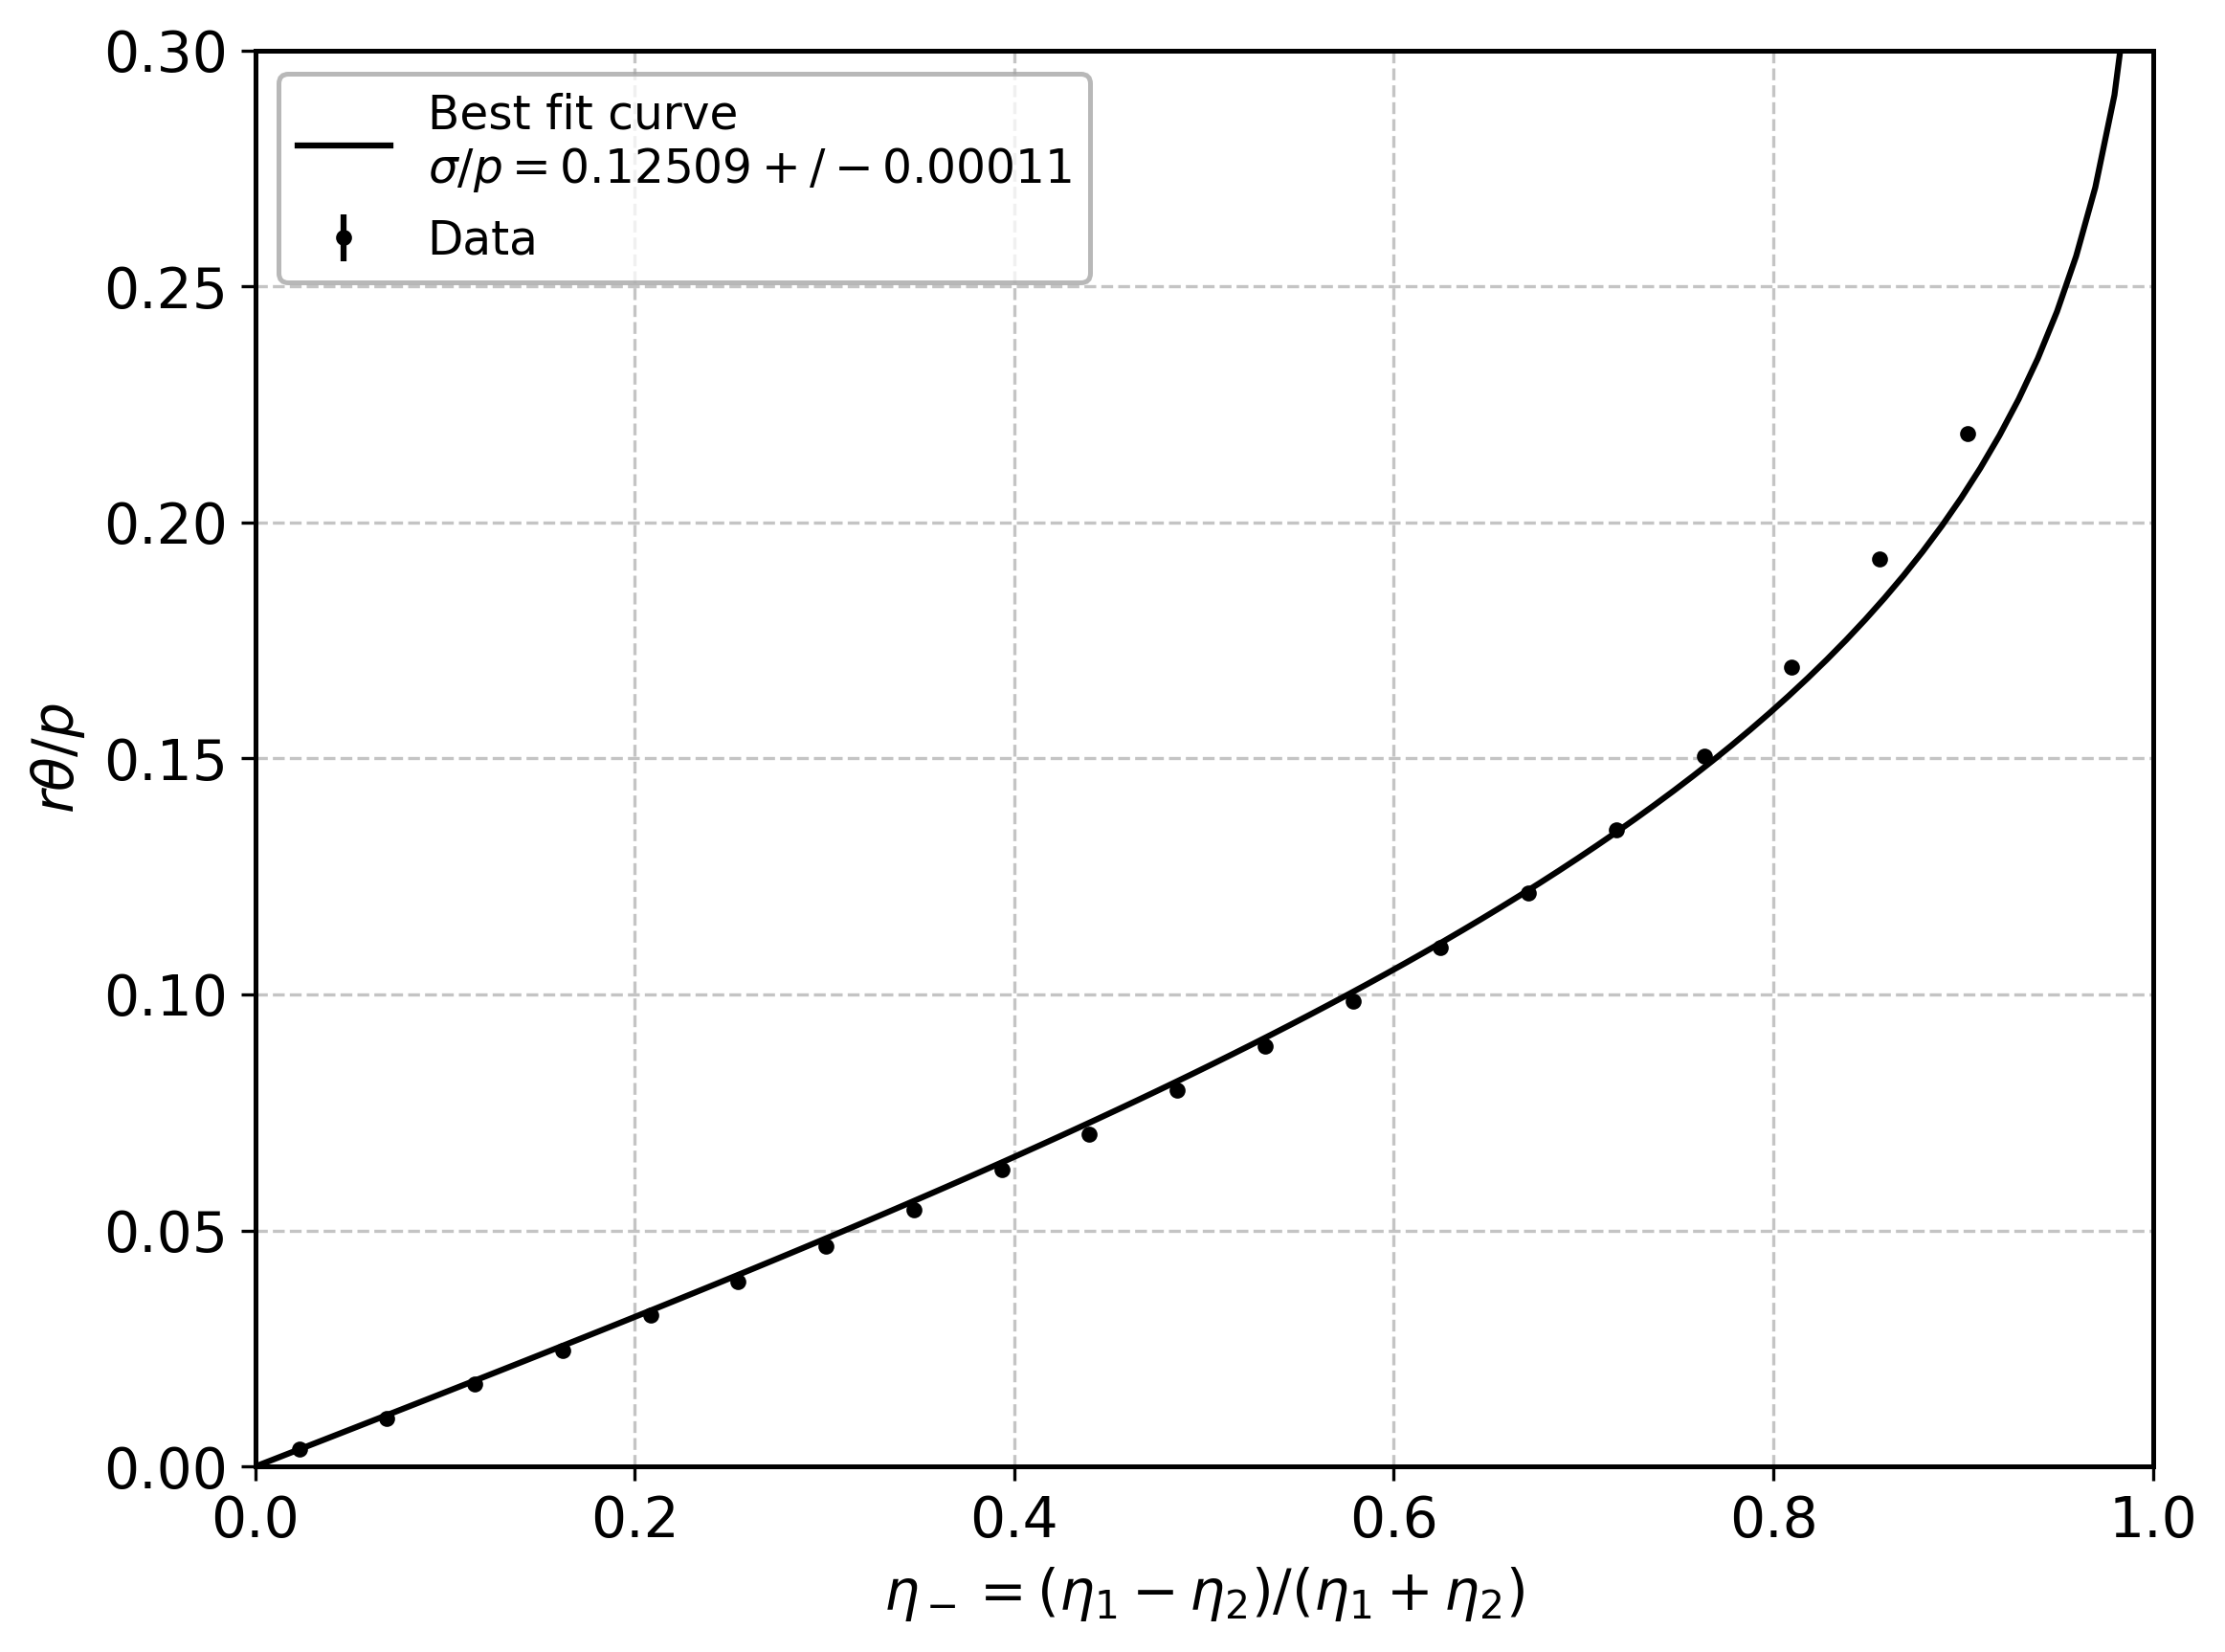
\includegraphics[width=0.49\linewidth]{figures/chapter4/position/eta_3pix_angular_fit}
    \caption{Profile and best-fit curves for the radial and angular components using Eqs. \ref{eq:eta_3pix_final} and \ref{eq:eta_3pix_ang_final}. The simulation has an estimated $\langle \sigma \rangle / p = 0.15$.}
    \label{fig:eta_3pix_fit}
\end{figure}

A small correction needs to be applied because Eq. \ref{eq:eta_3pix_no_final} does not take into account the hexagonal geometry of the pixels and that the internal angles of the hexagons are 120 degrees. Indeed, if a photon hits the vertex and the charge is equally divided between the three pixels, $\eta_+ = 2/3$ but $\Phi^{-1}(2/3) \neq 0$. As a consequence the impact point would not be reconstructed on the vertex, but outside the central pixel. The solution is to normalize $\eta_+$ in order to satisfy $r(2/3) = 1/\sqrt{3}$, thus the final model is
\begin{equation}
r(\eta_+) = \frac{p}{\sqrt{3}} + \sigma \Phi^{-1}\left( \frac{3}{4}\eta_+ \right).
\label{eq:eta_3pix_final}
\end{equation}

To find the model for the angular coordinate it is possible to consider only the two outer pixels, because $\eta_-$ is normalized with respect to the charge collected by these two pixels. The charge diffusion between these two pixels can be modeled as a one-dimensional Gaussian distribution centered in $y$, which is the distance from the midpoint of the pixels.

The relation between $\eta_-$ and $y$ can be found by calculating the fraction of Gaussian that falls inside each pixel, and is given by

\begin{equation}
\eta_-(y) = \frac{\eta_1}{\eta_+} - \frac{\eta_2}{\eta_+} = \left[1 - \Phi \left( - \frac{y}{\sigma} \right ) \right] - \Phi \left( - \frac{y}{\sigma} \right).
\label{eq:eta_3pix_ang}
\end{equation}
Using the approximation of small angles, the relation between the angular coordinate $\theta$ and $y$ is $\theta = y / r$. Inverting Eq. \ref{eq:eta_3pix_ang}, it is possible to find the relation between $\theta$ and $\eta_-$

\begin{equation}
\theta(\eta_-) =  - \frac{\sigma}{r} \Phi^{-1} \left( \frac{1 - \eta_-}{2} \right) = \frac{\sigma}{r} \Phi^{-1} \left( \frac{1 + \eta_-}{2} \right),
\label{eq:eta_3pix_ang_final}
\end{equation}
where it has been used that $\Phi^{-1}(1 - z) = - \Phi^{-1}(z)$.

To calibrate the radial and angular coordinates the strategy is identical to the calibration of two-pixels events. The projection onto the $\hat{r}$ axis and the angle with respect to it are calculated from Monte Carlo truth data of three-pixels events, then are binned in $\eta_+$ and $\eta_-$, and the median of the respective distributions are calculated. The resulting data are fitted with the respective models in Eqs. \ref{eq:eta_3pix_final} and \ref{eq:eta_3pix_ang_final}. Data and best-fit curves are shown in Fig. \ref{fig:eta_3pix_fit}.

As can be observed from Figs. \ref{fig:eta_2pix_r_distr} and \ref{fig:eta_3pix_fit}, the models describe very well the data, and the shape of the profiles are compatible with the cumulative distributions in Figs. \ref{fig:eta_2pix} and \ref{fig:eta_3pix} obtained with the unmodeled $\eta$ algorithm. This validates both the unmodeled and modeled algorithms, which converge to very similar results.

\begin{figure}[!b]
    \centering
    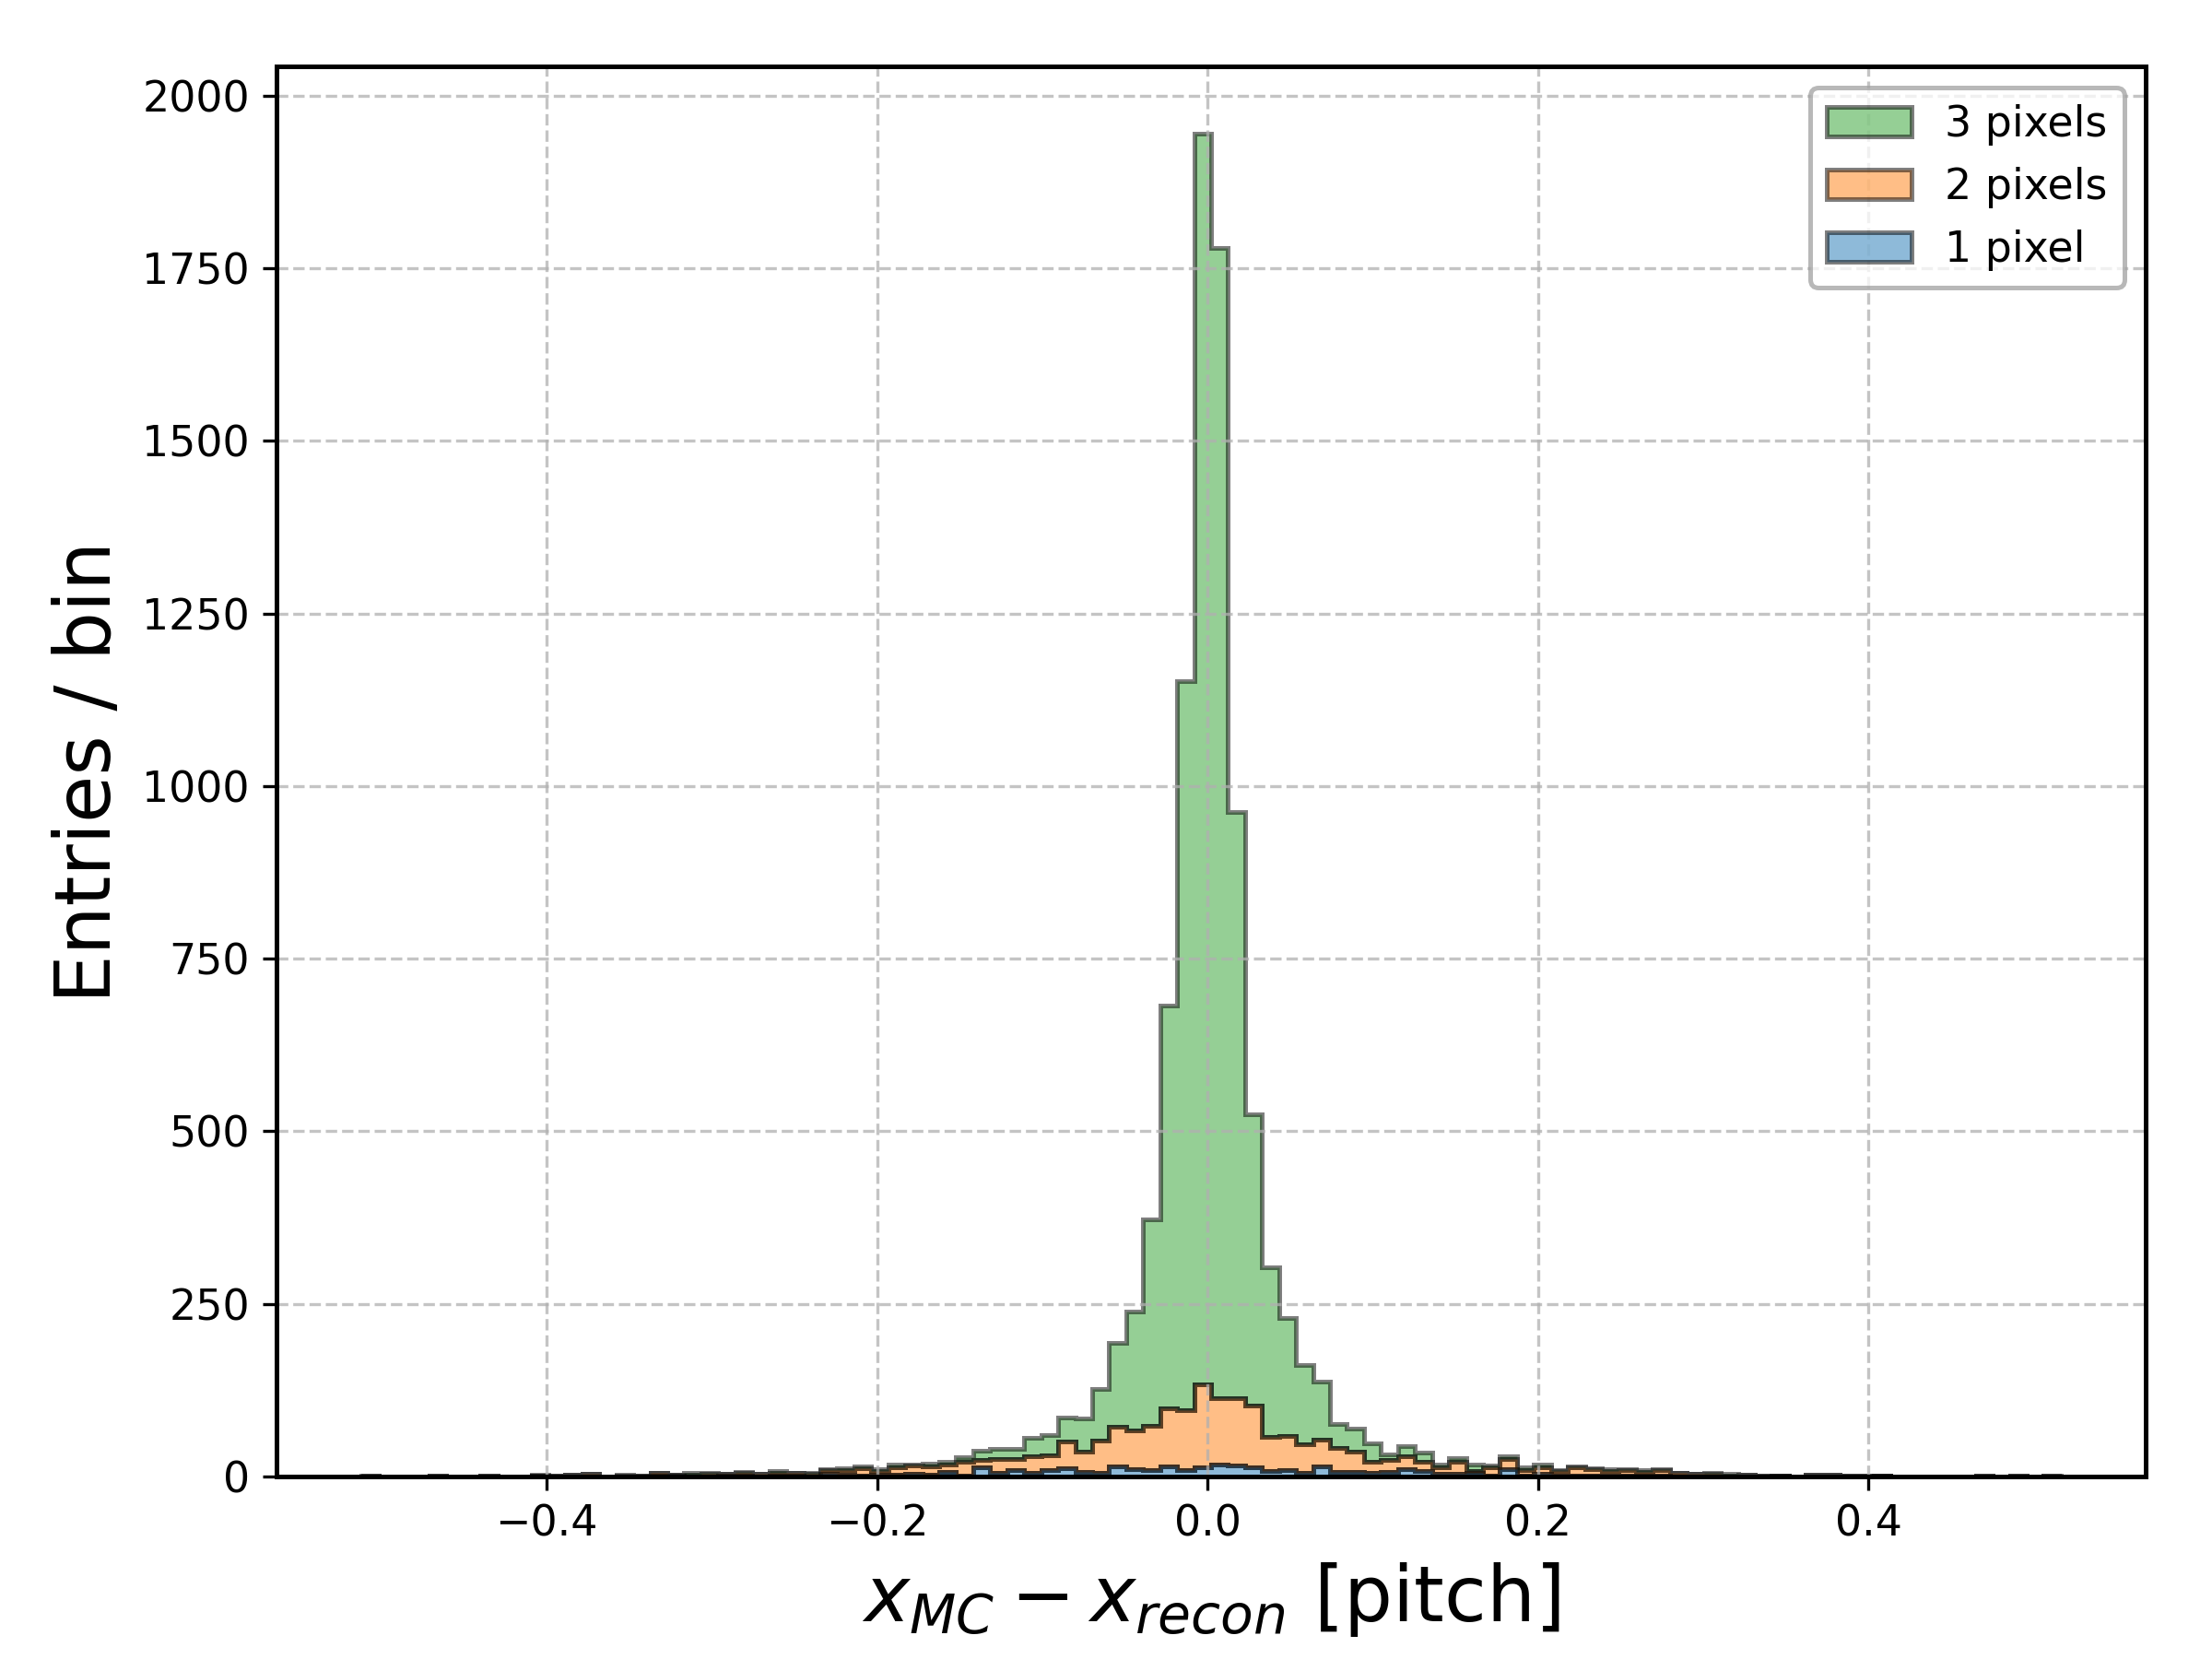
\includegraphics[width=0.49\linewidth]{figures/chapter4/position/eta_modeled_dx}
    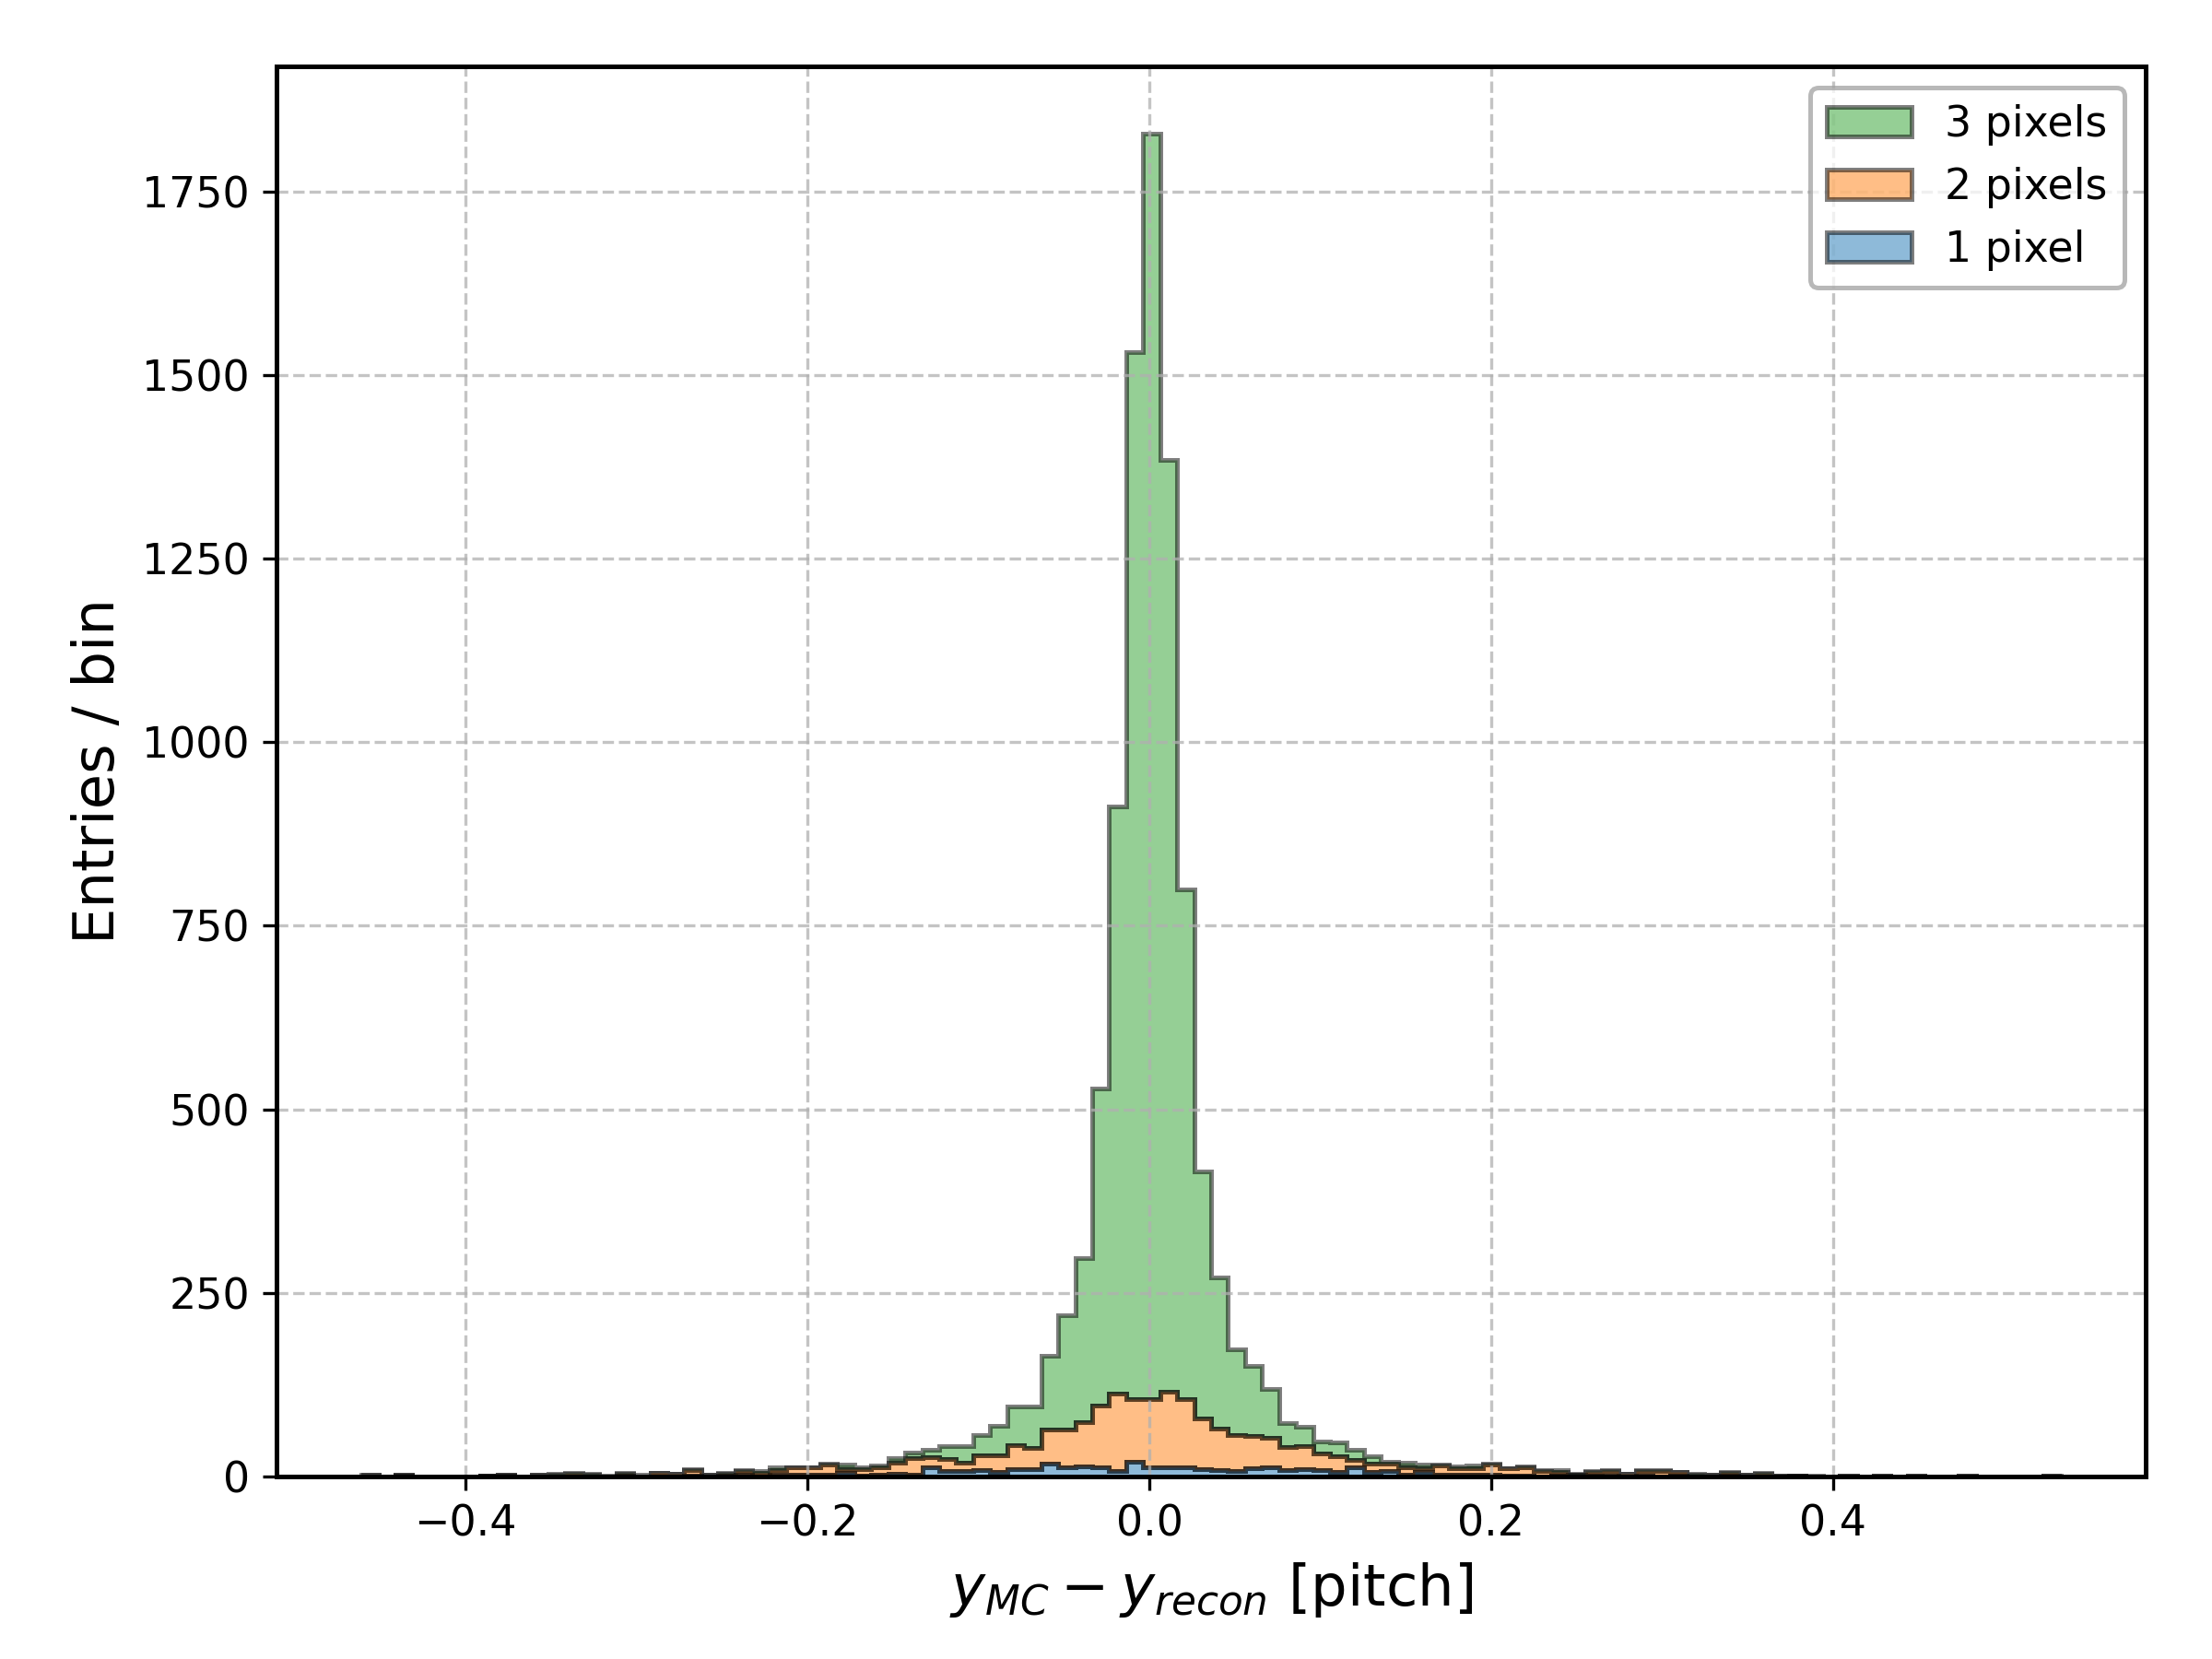
\includegraphics[width=0.49\linewidth]{figures/chapter4/position/eta_modeled_dy}
    \caption{Residuals distributions of the modeled eta algorithm for the $x$ and $y$ directions, calculated as the difference between the reconstructed and the Monte Carlo truth $x$ and $y$ components. The events are separated by cluster size, with each color representing a specific cluster size. The histograms are stacked on each other. The simulation is made with a 8 keV monochromatic source, 20 ENC of noise and ratio between the diffused charge cloud sigma and the pitch of 15\%.}
    \label{fig:eta_modeled_dx_dy}
\end{figure}

However, it can be noted that the best-fit values of $\sigma$ for the three fits are different. The simulation was performed with an average ratio $\langle \sigma \rangle / p = 0.15$, and only the parameter obtained from two-pixel events is compatible with the expected value. These discrepancies can be attributed to the spatial distribution of the events around the projection axes. Indeed, when this distribution is broad, as in the case of three-pixel events (Fig.~\ref{fig:3pix_scatter}), the deviation from the expected value is larger than for two-pixel events (Fig.~\ref{fig:2pix_scatter}). This must be taken into account, as calibration via Monte Carlo simulations becomes necessary, and the nominal value of $\langle \sigma \rangle /p$ estimated through Eqs. \ref{eq:z_average} and \ref{eq:diff_sigma_dist} cannot be directly used.

Once the best-fit parameters have been estimated from simulations, a separate dataset can be analyzed and the resulting residuals distributions are shown in Fig. \ref{fig:eta_modeled_dx_dy}. As for the other cases where the physics of charge diffusion has been taken into account, the resulting distributions are narrow and unimodal.

Moreover, the EEF of the modeled $\eta$ algorithm is very steep and has less relevant tails with respect to the MLE algorithm, as visible in Fig. \ref{fig:eta_modeled_eef}. As expected, the EEF becomes steeper for larger diffusion widths. 
%The distances at which the EEF contains 50\% and 90\% of the events are listed in Tab. \ref{tab:eta_modeled_eef}.

\begin{figure}[h]
    \centering
    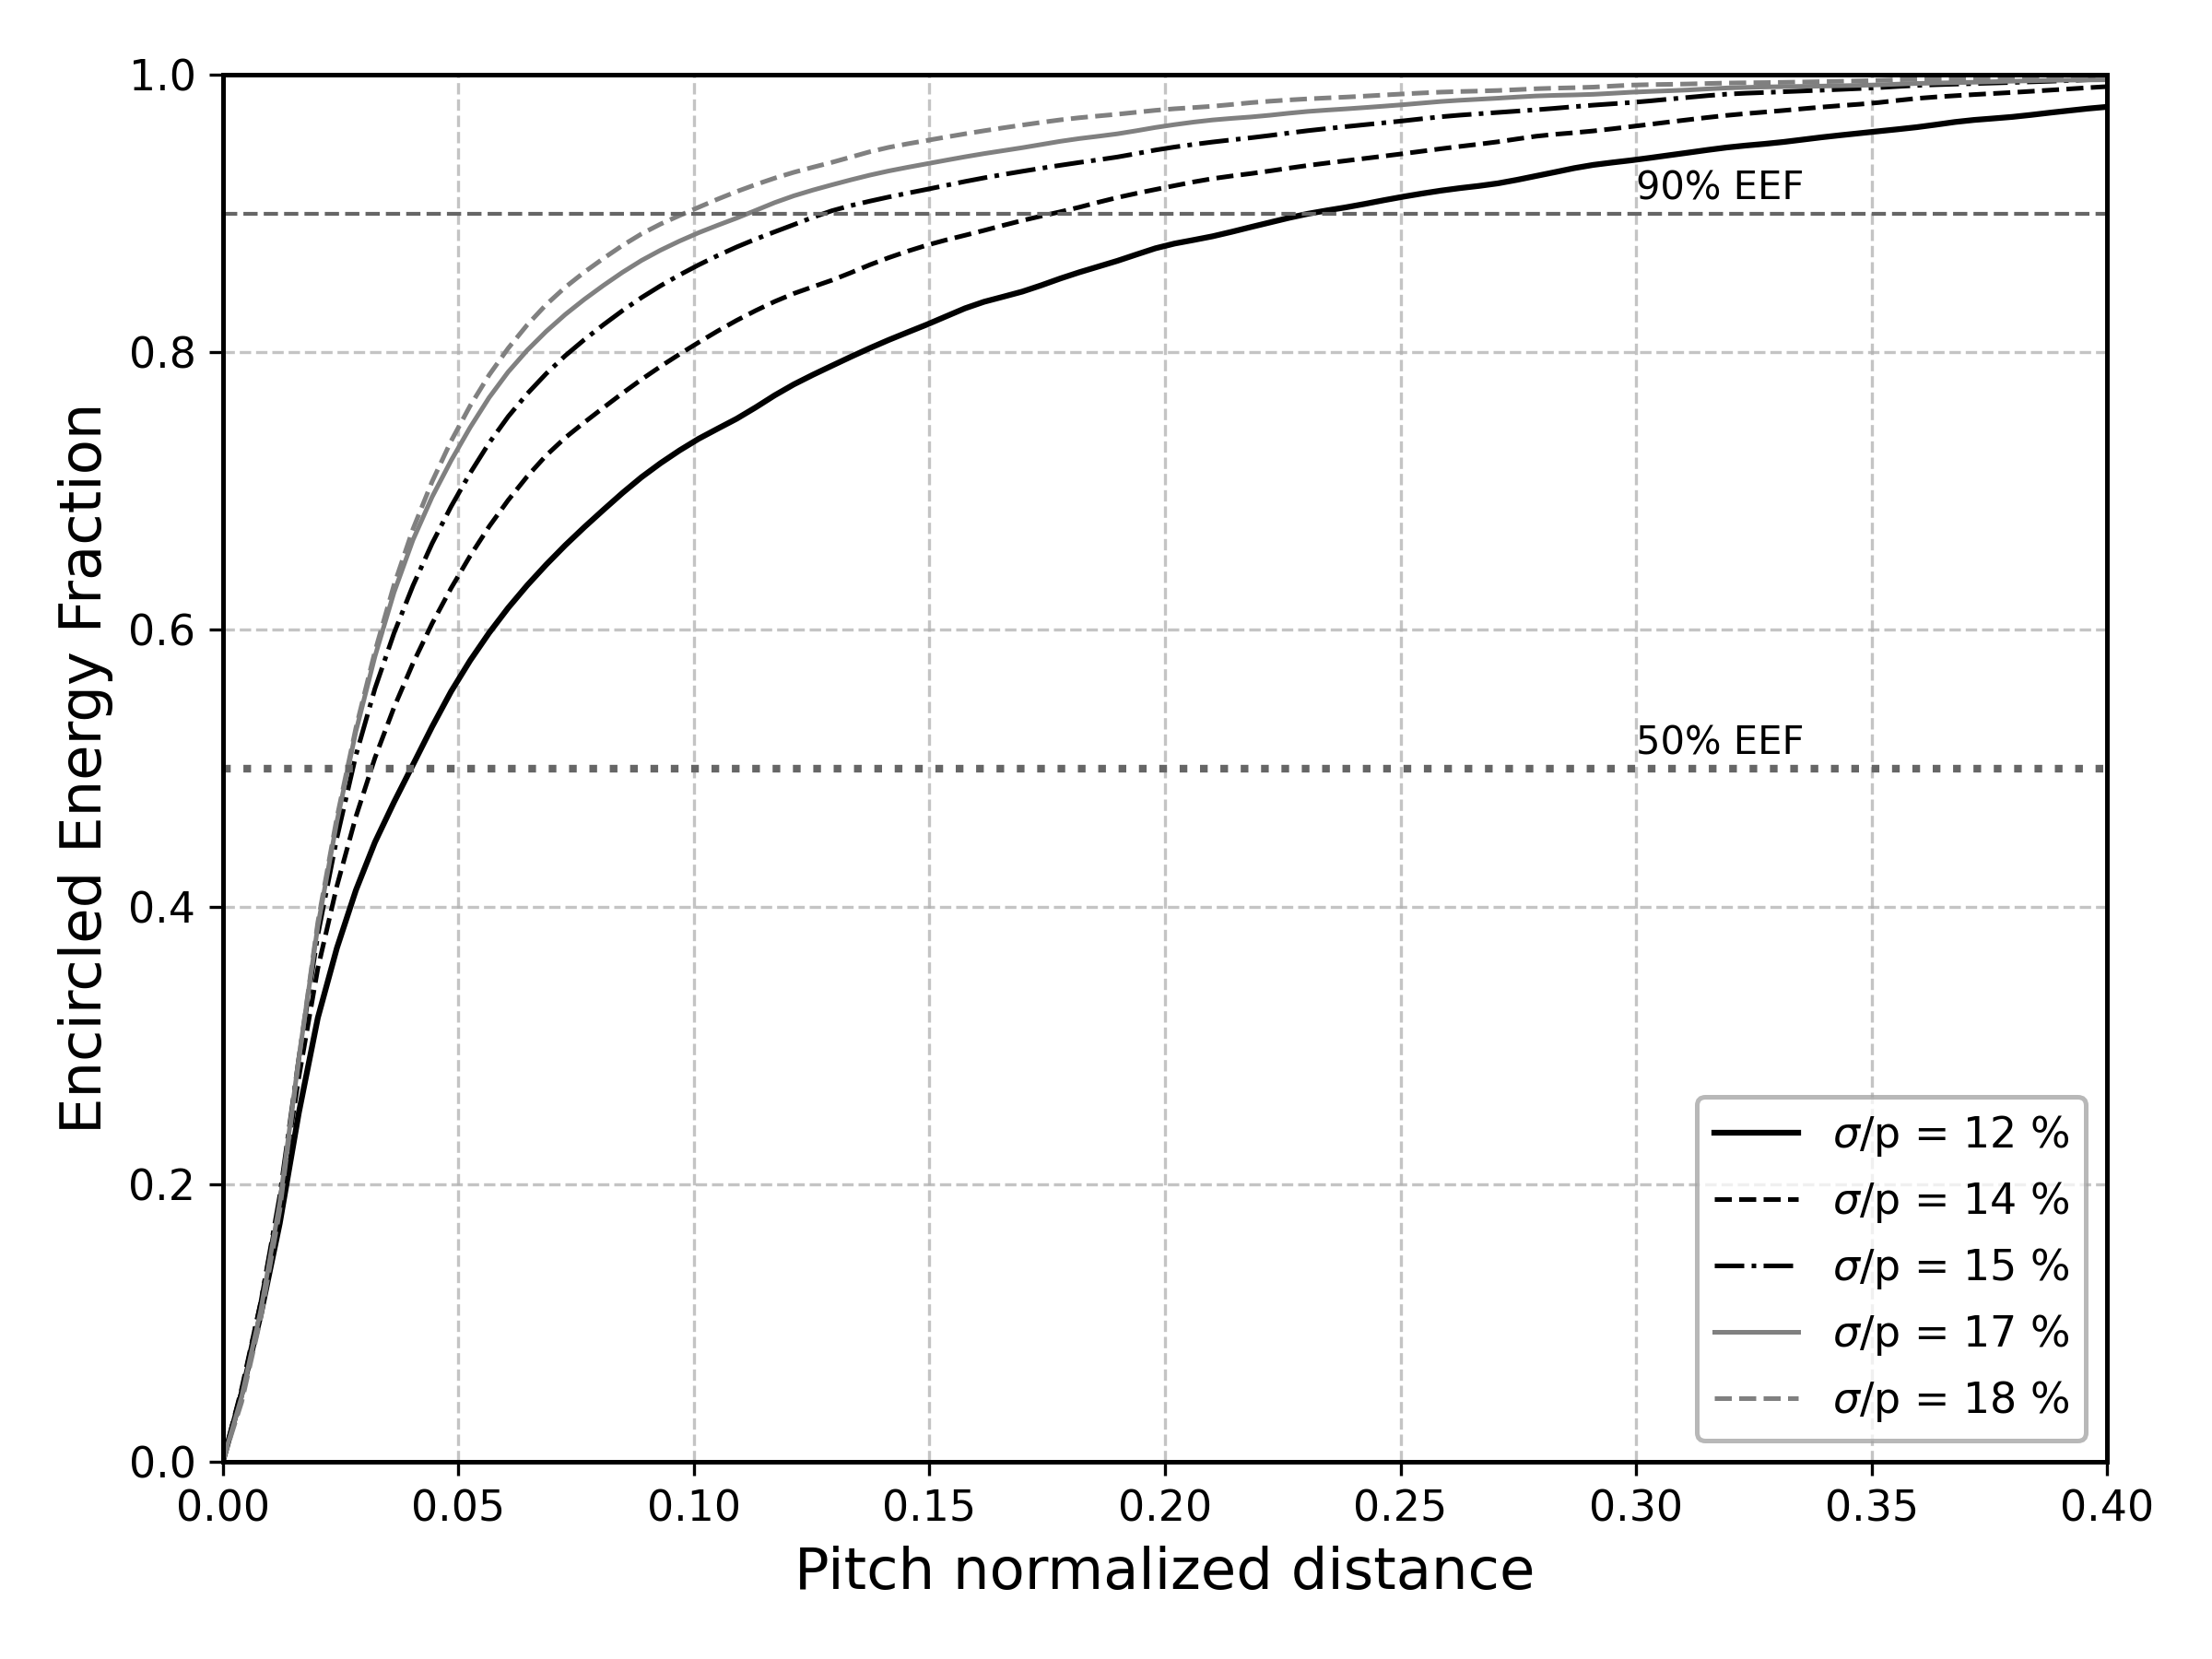
\includegraphics[width=0.7\linewidth]{figures/chapter4/position/eta_modeled_eef}
    \caption{Encircled energy fraction of the modeled eta reconstruction for different values of the ratio between the diffused charge cloud and the pixel pitch as a function of the pitch normalized distance. The simulation is made with 20 ENC of noise.}
    \label{fig:eta_modeled_eef}
\end{figure}

%\begin{table}[htbp]
%\centering
%\begin{tabular}{c cccc}
%$\langle \sigma \rangle / p$ & EEF@50\% [pitch] & EEF@90\% [pitch]\\
%\midrule
%12.2 & 0.04 & 0.23 \\
%13.7 & 0.03 & 0.18 \\
%15.2 & 0.03 & 0.13 \\
%16.8 & 0.03 & 0.11 \\
%18.3 & 0.03 & 0.10 \\
%\bottomrule
%\end{tabular}
%\caption{Pitch distances at which EEF contains 50\% and 90\% of the events with modeled eta reconstruction, as a function of the ratio $\langle \sigma \rangle / p$. The values are extracted from Fig. \ref{fig:eta_modeled_eef}}
%\label{tab:eta_modeled_eef}
%\end{table}

\subsection{Algorithms comparison}
\label{subsec:position_comparison}

To summarize and compare the results of the different reconstruction algorithms, Fig. \ref{fig:eef} shows the values of EEF@50\% and EEF@90\% as a function of the $\langle \sigma \rangle / p$ ratio for all the discussed methods.

\begin{figure}[htbp]
    \centering
    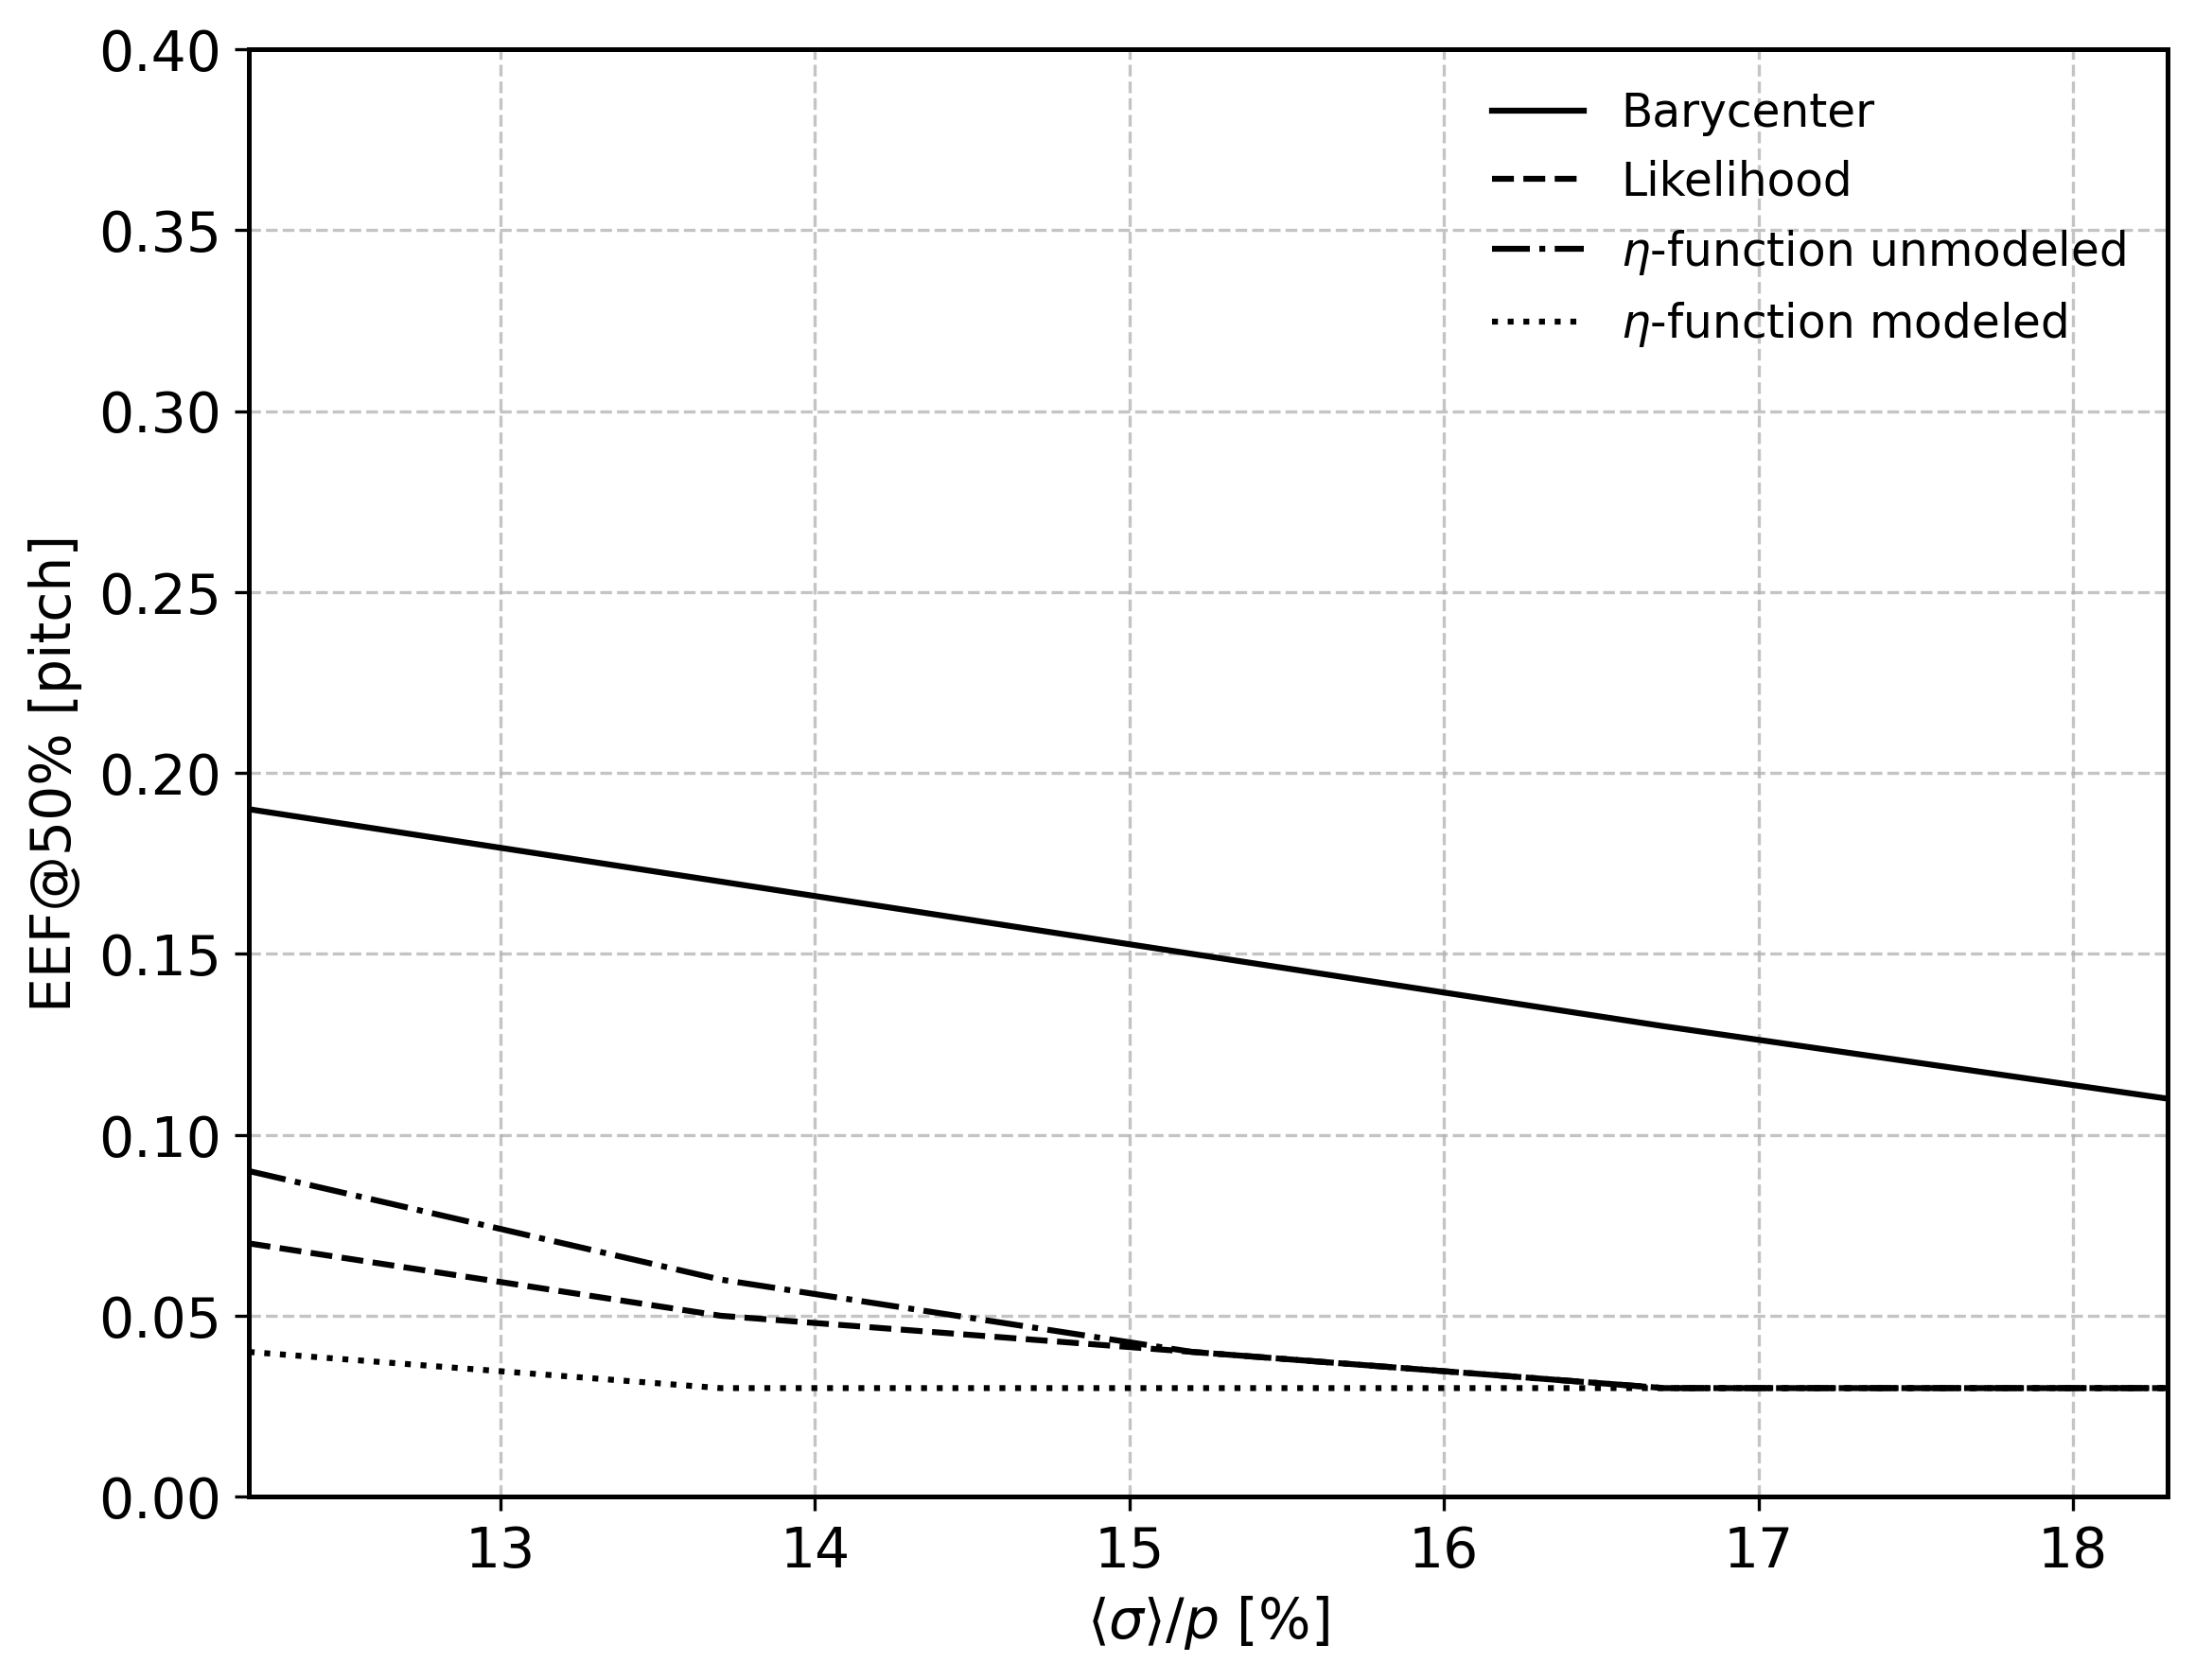
\includegraphics[width=0.49\linewidth]{figures/chapter4/position/eef50}
    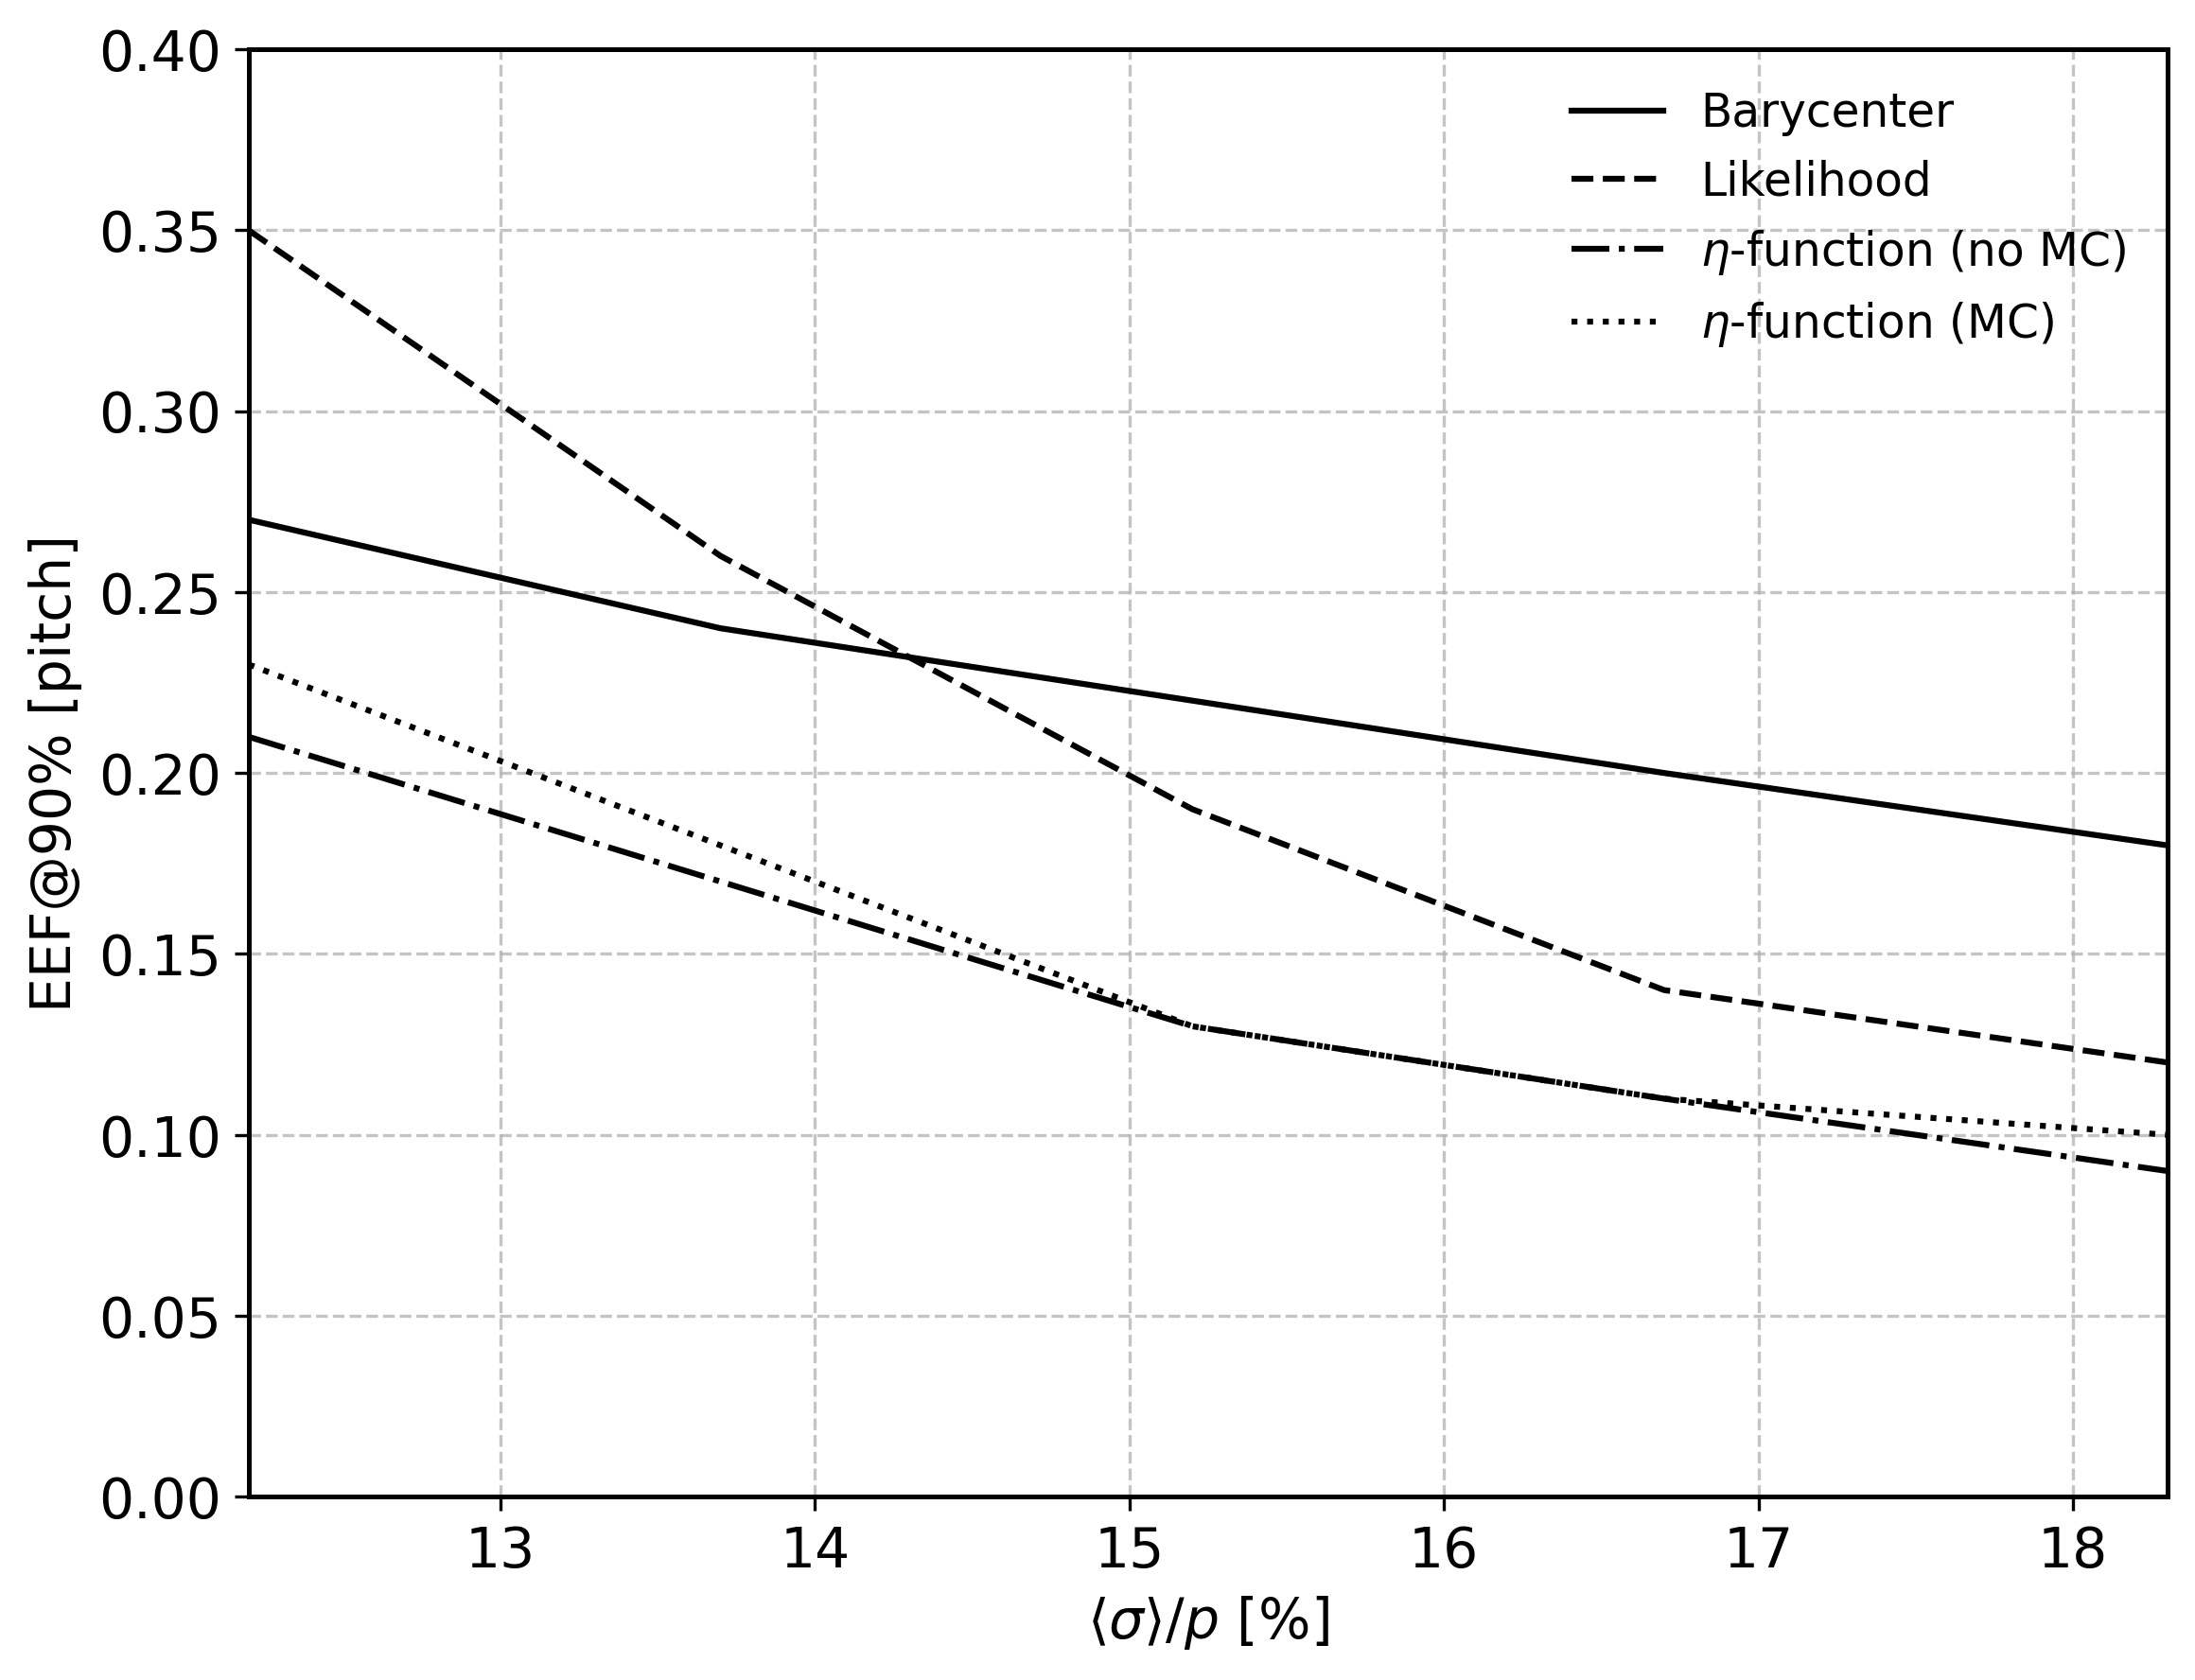
\includegraphics[width=0.49\linewidth]{figures/chapter4/position/eef90}
    \caption{EEF at 50\% (left panel) and 90\% (right panel) as a function of the ratio between the diffusion cloud sigma and the pixel pitch for all the position reconstruction algorithms. All the values are normalized to the pixel pitch.}
    \label{fig:eef}
\end{figure}

As visible in the left panel, the charge barycenter gives the worst core resolution for all diffusion regimes, with values of the EEF@50\% between 0.11 and 0.19 pitch. On the other hand, the MLE and the modeled $\eta$ algorithms achieve the best core containment, improving the EEF@50\% by up to a factor of four with respect to the charge barycenter. The unmodeled $\eta$ algorithm shows slightly worse results than the modeled one for small diffusion widths, but reaches identical values for broader diffusions.

Considering the tails of the distributions, shown in the right panel with the EEF@90\%, the situation is different. For small values of $\langle \sigma \rangle / p$, the MLE has very long tails and its EEF@90\% is even worse than the charge barycenter. This does not happen for the $\eta$ algorithms, which maintain better tail containment across all diffusion regimes. Between the two, the modeled $\eta$ algorithm achieves the best overall performance.

%\begin{figure}[htbp]
%    \centering
%    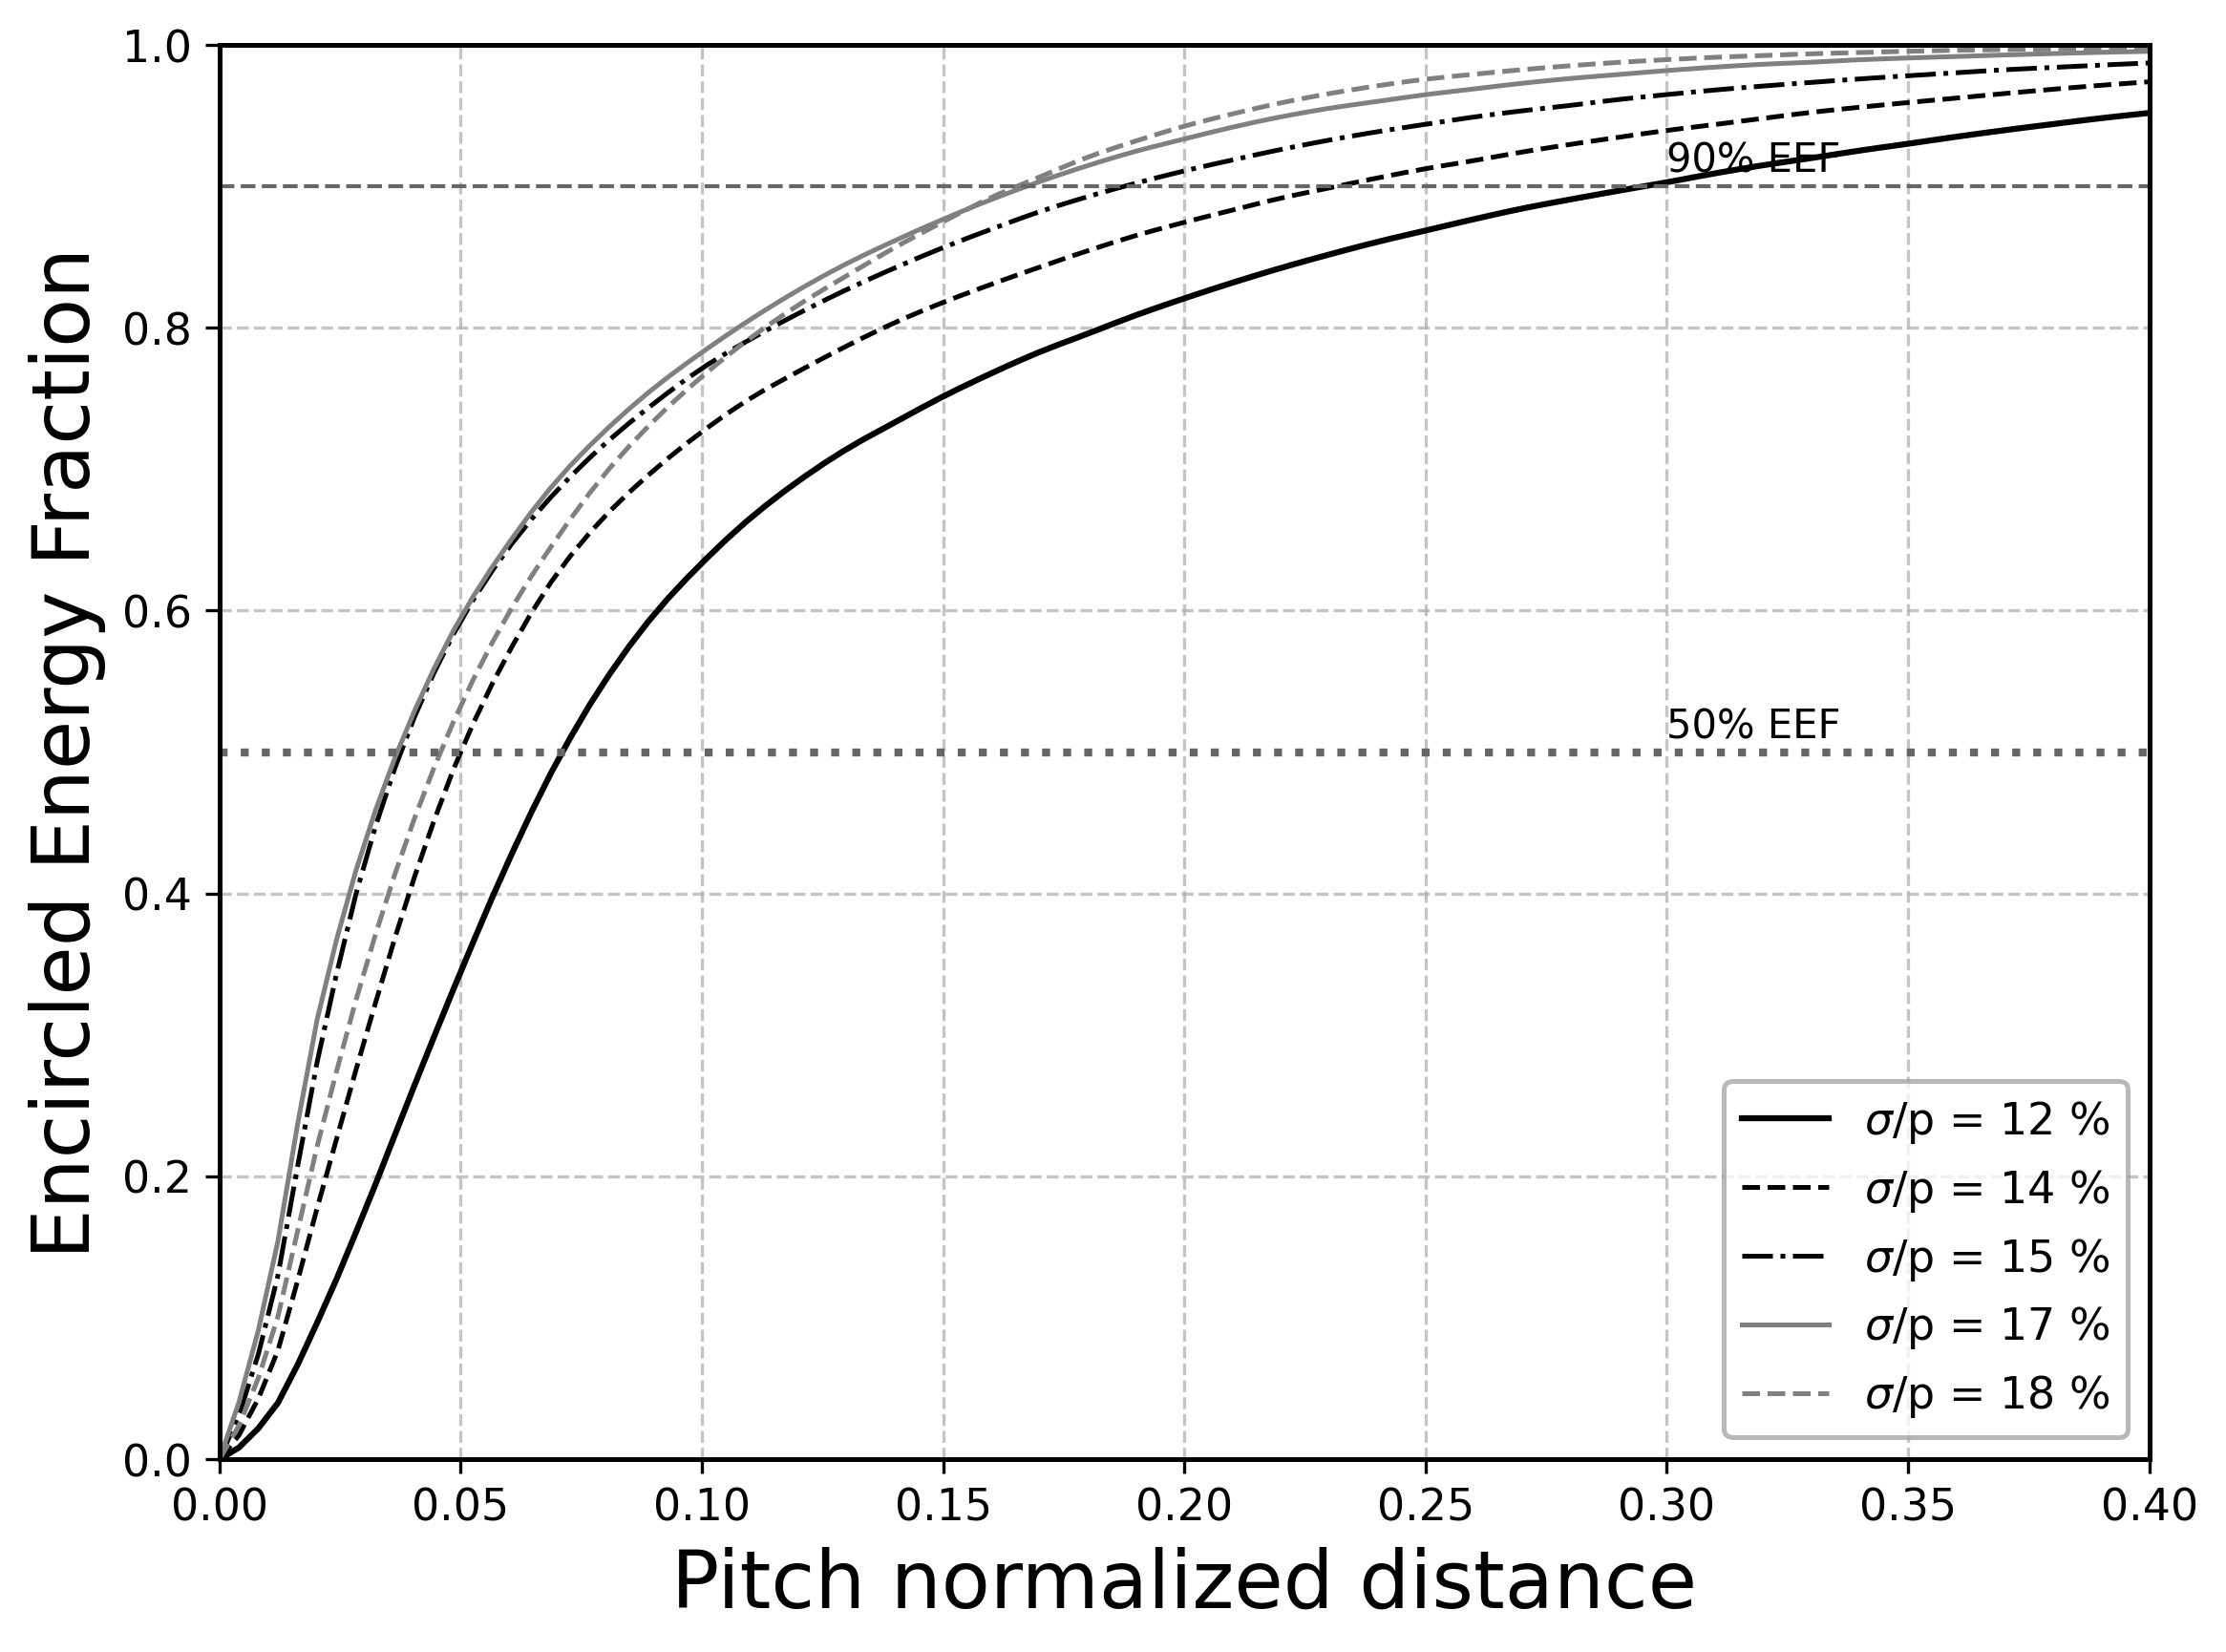
\includegraphics[width=0.49\linewidth]{figures/chapter4/position/mle_systematics}
%    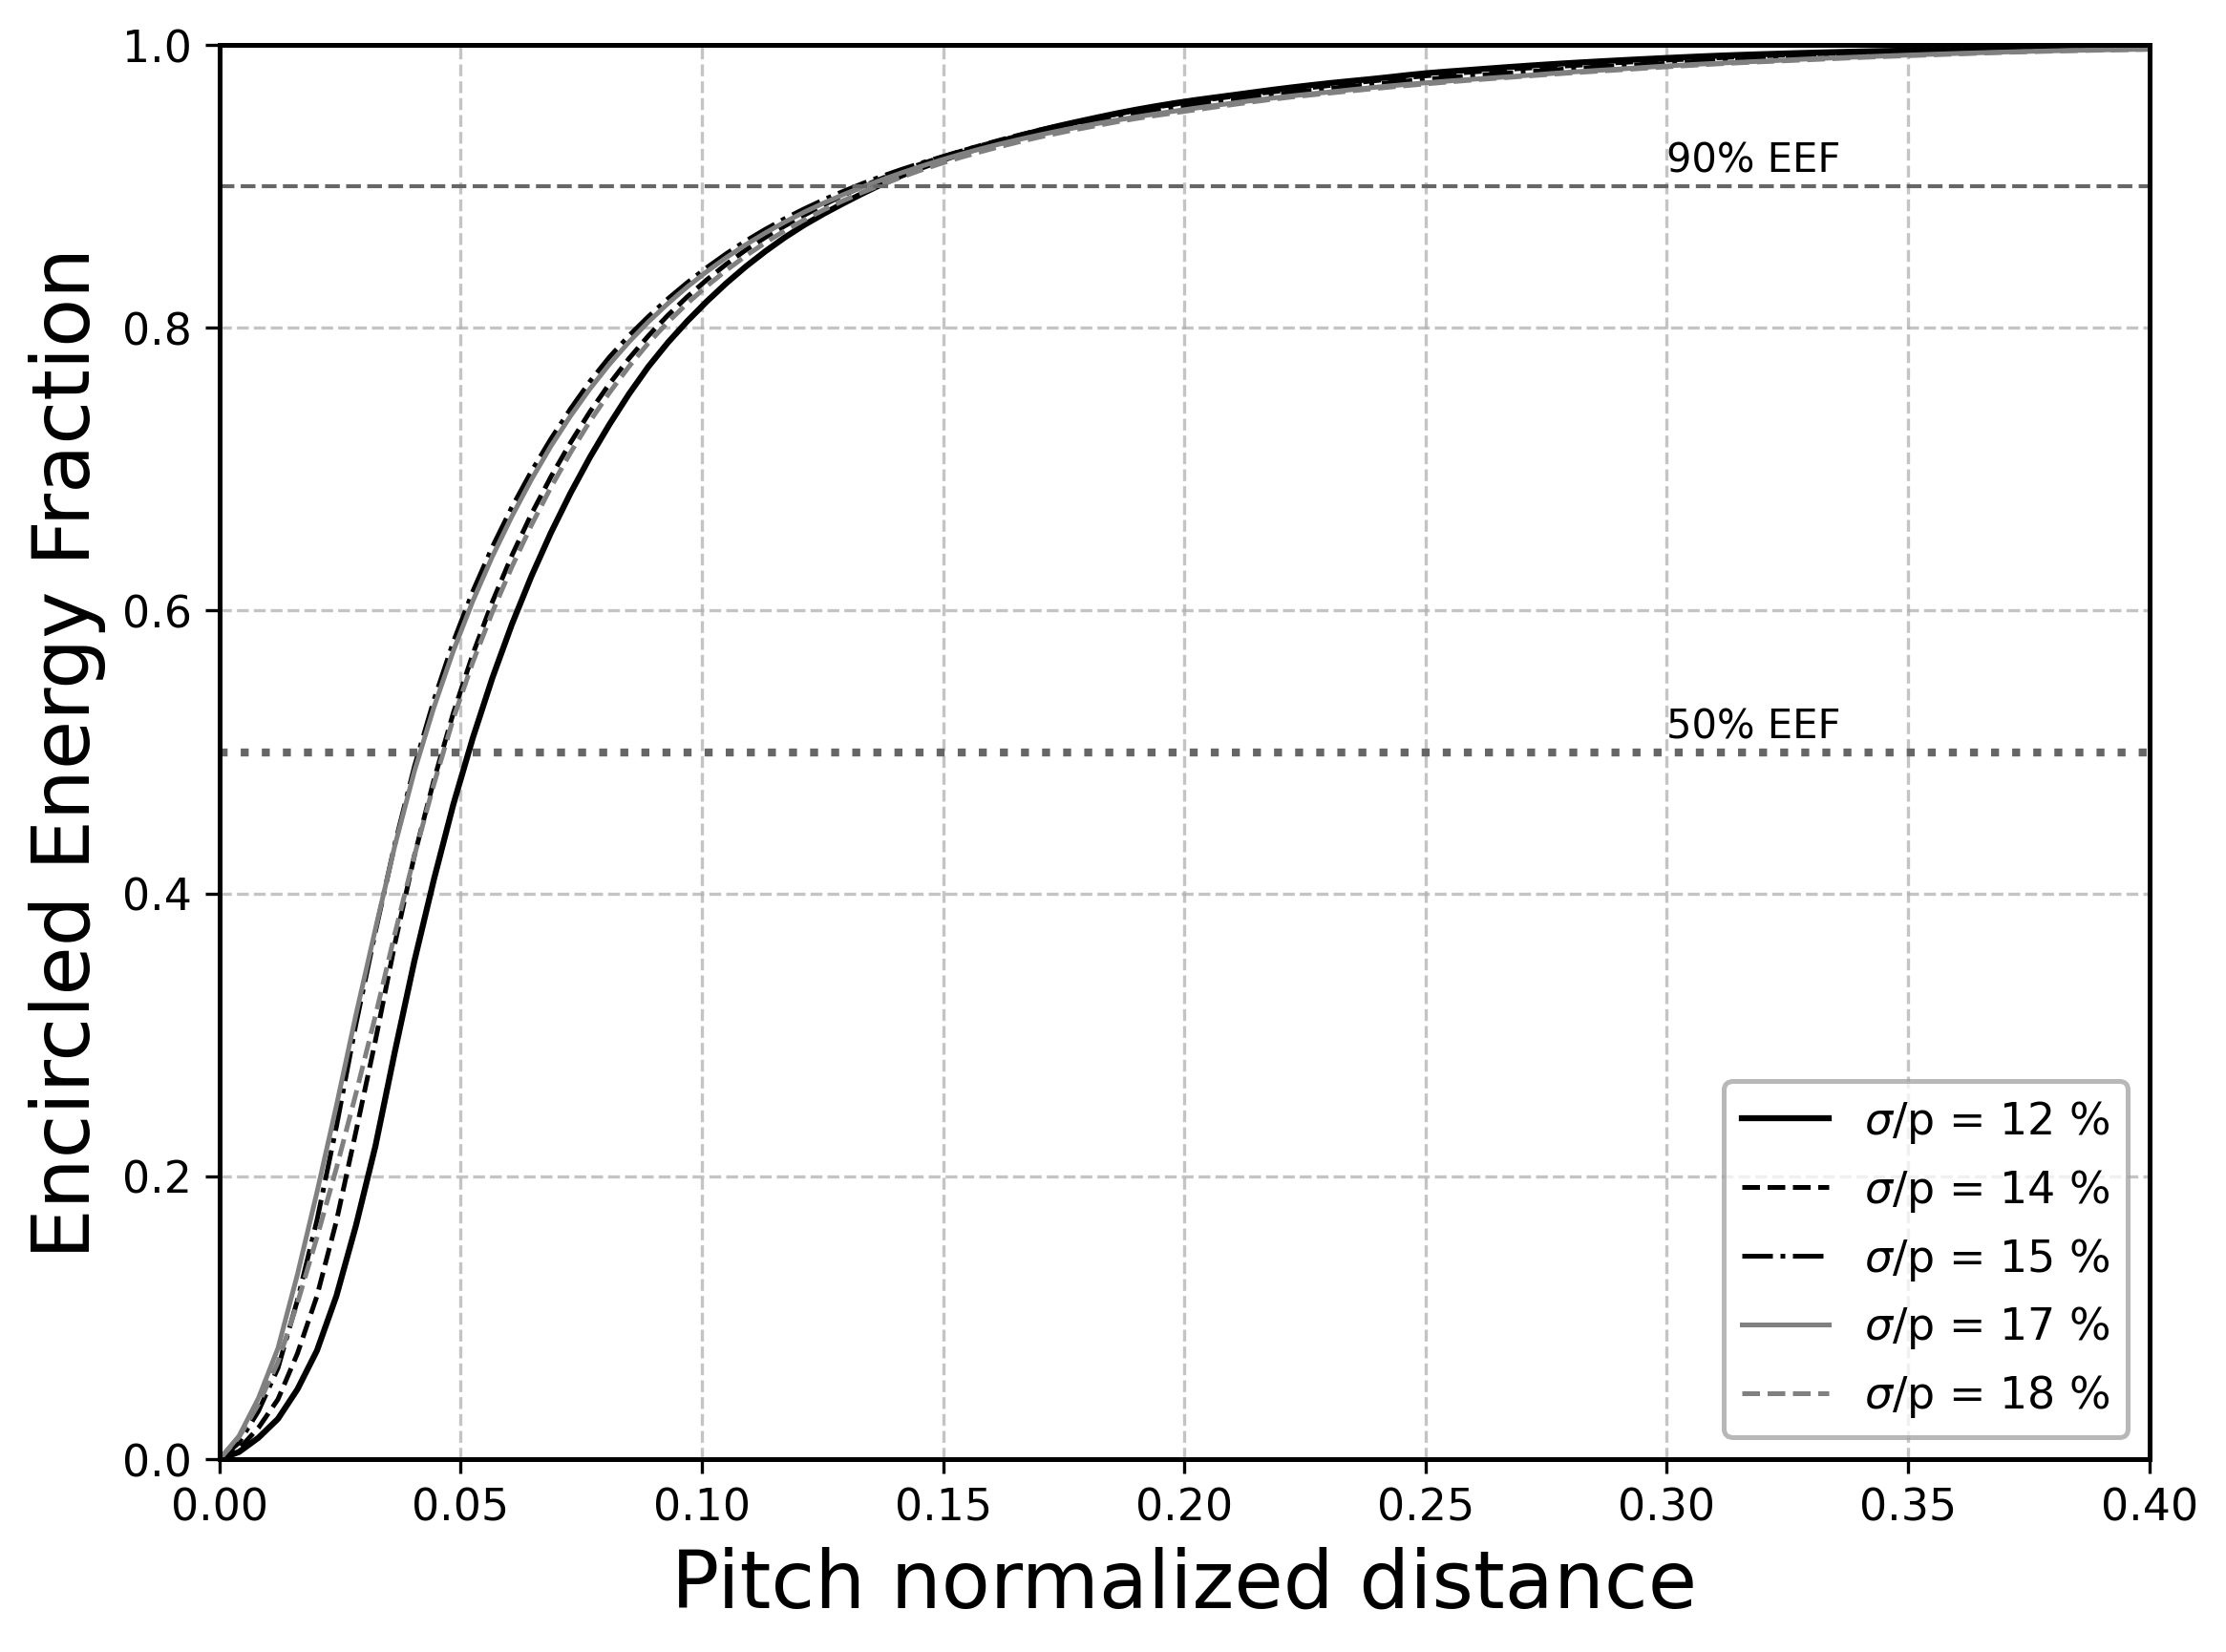
\includegraphics[width=0.49\linewidth]{figures/chapter4/position/eta_unmodeled_systematics}
%    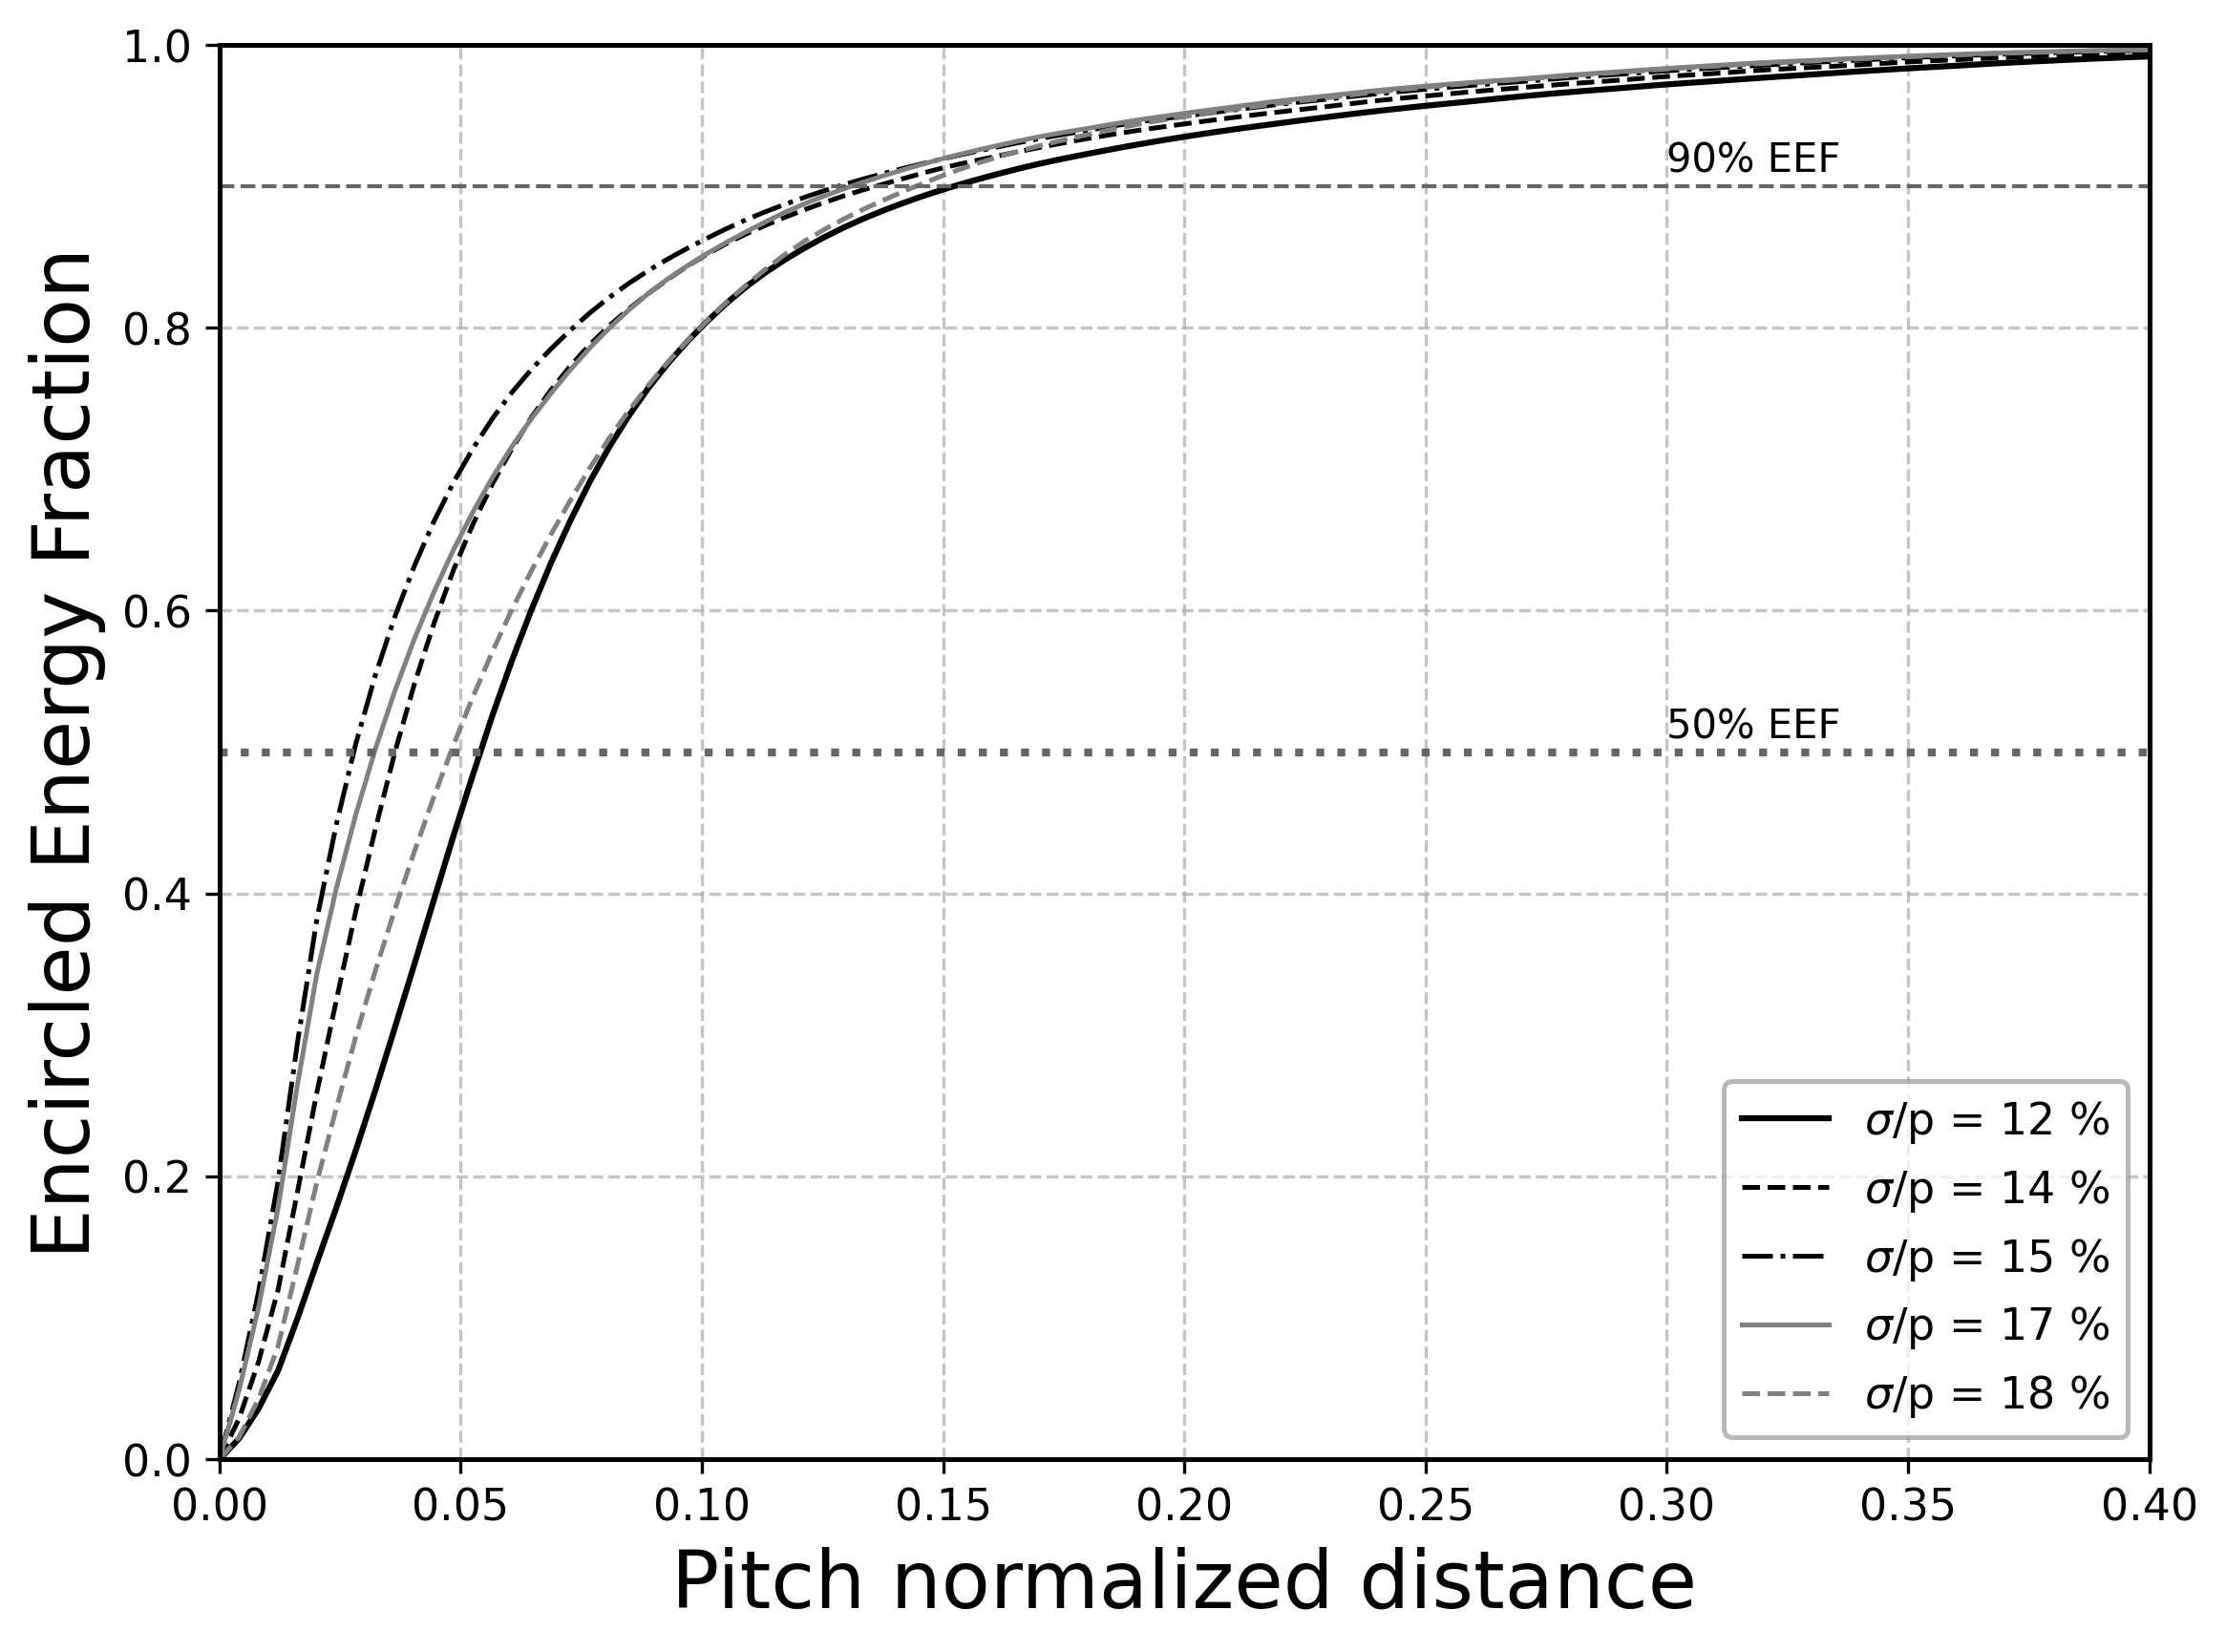
\includegraphics[width=0.49\linewidth]{figures/chapter4/position/eta_modeled_systematics}
%    \caption{}
%    \label{fig:eef_systematics}
%\end{figure}

Both the MLE and the modeled $\eta$ algorithms require an accurate calibration from Monte Carlo simulations, while the unmodeled $\eta$ relies on data from a uniform illumination. In a real scenario, systematic uncertainties in the Monte Carlo parameters can introduce an error in the assumed charge diffusion width.

To quantify how this mismatch affects the spatial resolution, the simulated dataset with a true $\langle \sigma \rangle / p = 15\%$ has been analyzed using "wrong" calibrations generated for different values of $\langle \sigma \rangle / p$. The relative variation of the EEF is reported in Tab. \ref{tab:variation_eef}.

The results show that the MLE and the modeled $\eta$ algorithms are very sensitive to calibration errors. If the diffusion width is not exact, the core resolution drastically worsens, with the EEF@50\% increasing up to almost 90\% for the MLE. On the other hand, the unmodeled $\eta$ algorithm is much more stable. Even with a large mismatch, its core resolution degrades by a maximum of 25\%, and its tails (EEF@90\%) are almost completely unaffected. This means that if Monte Carlo simulations are not perfectly tuned, the unmodeled $\eta$ algorithm is the most reliable choice.

\begin{table}[!t]
\centering
\begin{tabularx}{\textwidth}{X ccccc}

Reconstruction Algorithm & \multicolumn{5}{c}{$\langle \sigma \rangle / p$ [\%]} \\
\cmidrule(l){2-6}
 & 12 & 14 & 15 & 17 & 18 \\
\midrule
MLE & & & & & \\
\quad EEF@50\% & 189\% & 133\% & 100\% & 98\%  & 122\% \\
\quad EEF@90\% & 157\% & 124\% & 100\% & 89\%  & 88\%  \\
\midrule
Unmodeled $\eta$ & & & & & \\
\quad EEF@50\% & 125\% & 112\% & 100\% & 101\% & 112\% \\
\quad EEF@90\% & 103\% & 101\% & 100\% & 101\% & 103\% \\
\midrule
Modeled $\eta$ & & & & & \\
\quad EEF@50\% & 194\% & 131\% & 100\% & 115\% & 172\% \\
\quad EEF@90\% & 119\% & 106\% & 100\% & 102\% & 112\% \\
\bottomrule
\end{tabularx}
\caption{Relative variation of the EEF@50\% and EEF@90\% obtained by analyzing a dataset with true $\langle \sigma \rangle / p = 15\%$ using calibrations generated with different diffusion widths. Values are normalized to the optimal calibration at 15\%, which corresponds to 100\%.}
\label{tab:variation_eef}
\end{table}

\subsection{Modulation transfer function}
\label{subsec:mtf}

A method that is commonly applied in medical physics to characterize the imaging response of the detector is to produce the image of a linear object and study the detector response. This can be achieved using an absorber material plate, such as lead for X-rays, with a slit on it \cite{fujita1992}. The intensity profile of the image on the axis perpendicular to the slit as a function of the position is then calculated, and the result is called Line Spread Function (LSF) \cite{med_imaging}. More precisely, the LSF is the convolution of the PSF with the slit

\begin{equation}
\operatorname{LSF}(x) = \operatorname{PSF}(x, y) \ast \operatorname{Slit}(x, y).
\end{equation}

To correctly characterize the LSF, the slit profile should approach a Dirac $\delta$-function, or at least the slit width should be much smaller than the expected resolution.

Another requirement for a better characterization is that the slit should be inclined with respect to the detector principal axes and the reason for this varies depending on the detector type. In case of energy integrating detectors, like those commonly used in radiography, the reason is that a slit aligned to an axis would produce a narrow LSF profile only a few pixels wide, thus it would be under-sampled. Instead, using an inclined slit causes pixels in adjacent rows to be hit in different positions, allowing to sample the LSF with sub-pixel sampling, which is called presampled LSF.

For single-photon driven readout detectors like ASIX, for which each photon is independently reconstructed with sub-pixel resolution, the reason to use a tilted slit is to uniformly sample the pixel. This enables to estimate the average resolution of the detector for the entire pixel, not only for a specific region. An example of the geometry of the detector and the slits is shown if Fig. \ref{fig:hex_grid_slits}.

The typical angle of the slit should be small, between 2 and 8 degrees, and should be far from being aligned to the main axes of the detector.

\begin{figure}[htbp]
    \centering
    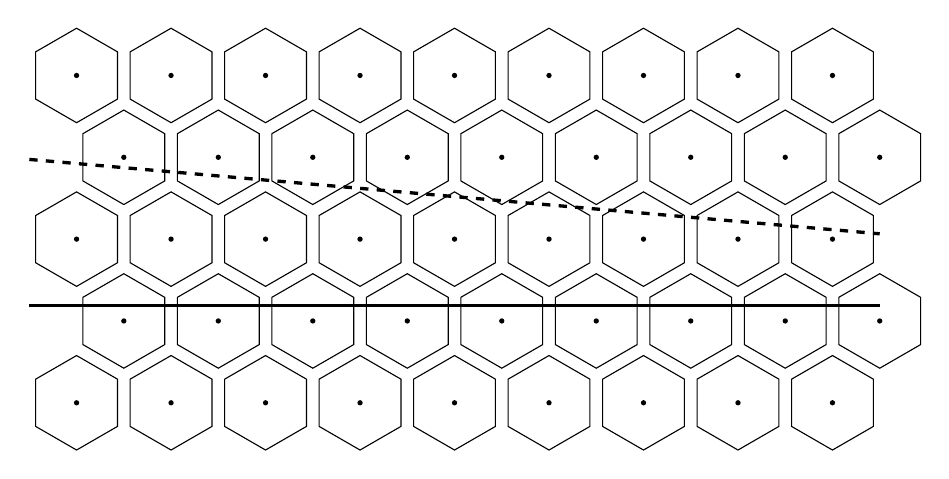
\begin{tikzpicture}[scale=1.2]
    
    \foreach \row in {-2,-1,0,1,2} {
        \foreach \col in {-4,-3,-2,-1,0,1,2,3,4} {
            \pgfmathsetmacro{\xpos}{\col + 0.5*mod(abs(\row),2)}
            \pgfmathsetmacro{\ypos}{\row * 0.866025}

            \hexpix[xshift=\xpos cm, yshift=\ypos cm]{\hexsize}
        }
    }

	\tikzset{slitLine/.style={very thick, opacity=0.7}}
	\draw[very thick, black] (-4.5, -0.7) -- (4.5, -0.7);;
	\draw[very thick, black, dashed] (-4.5, 0.84375) -- (4.5, 0.05625);

    \end{tikzpicture}
    \caption{Example of a grid with hexagonal pixels with two slits passing above. The solid line represents a slit parallel to the horizontal axis of the detector and always crosses the pixels in the same region. The dashed line represents an inclined slit with an angle of 5 degrees, and it crosses different regions each time.}
    \label{fig:hex_grid_slits}
\end{figure}

Producing a slit with a width small enough for high-resolution detectors is not always possible. An alternative method to characterize the spatial resolution consists of using the sharp edge of a slab of absorber material.

The profile image of the transition region around the edge is called Edge Spread Function (ESF). As for the slit method, the edge method requires the edge to be slightly tilted with respect to the main axes of the detector. Similarly to the LSF, the ESF can be computed as

\begin{equation}
\operatorname{ESF}(x) = \operatorname{PSF}(x, y) \ast \operatorname{Edge}(x, y).
\end{equation}

The ideal edge should be perfectly sharp to not introduce distortions, thus it can be represented with a step function. Using the convolution properties, it is possible to show that the derivative of the ESF corresponds to the LSF

\begin{equation}
\frac{d}{dx} \operatorname{ESF}(x) = \operatorname{PSF}(x, y) \ast \frac{d}{dx} \operatorname{Edge}(x, y) = \operatorname{PSF}(x, y) \ast \operatorname{Line}(x, y) = \operatorname{LSF}(x).
\label{eq:esf_lsf}
\end{equation}

This relation holds also when the edge is not ideal.

Once the LSF has been sampled, either directly with a slit or indirectly with an edge using Eq. \ref{eq:esf_lsf}, it is possible to characterize the profile to determine the spatial resolution, that can be defined as the FWHM of the LSF.

The LSF and ESF are defined in the spatial domain. There is another quantity that is commonly used to characterize the imaging properties of a detector which is defined in the frequency domain, the modulation transfer function (MTF). The MTF is defined as the Fourier transform of the LSF

\begin{equation}
\operatorname{MTF}(f) = \mathcal{F}(\operatorname{LSF}(x)).
\label{eq:mtf}
\end{equation}

By definition, the amplitude of MTF is normalized in order to have $\operatorname{MTF}(0) = 1$, which can be achieved either by normalizing the LSF area to 1 or by dividing the resulting MTF by $\operatorname{MTF}(0)$.

The MTF measures how the contrast is transfered as a function of the spatial frequency of the incoming signal. A high value of the MTF for higher frequencies means that the detector has high contrast, thus it can resolve small objects. For an ideal detector with infinite resolution the LSF is a Dirac-$\delta$ function and the resulting MTF is constant and equal to 1.

As for the LSF and the ESF, using a tilted slit or edge to increase the sampling frequency enables to compute the presampled MTF \cite{samei1998}. The usual metric used to determine the spatial resolution of a detector is related to the frequency $f_{10}$ for which $\operatorname{MTF}(f_{10}) = 0.1$.

If the LSF is described by a Gaussian curve $f_{10}$ can be related to its standard deviation. By considering that the Fourier transform of a Gaussian is still a Gaussian

\begin{equation}
\mathcal{F} \left( \frac{1}{\sqrt{2 \pi}\sigma} e^{-x^2/2\sigma^2 } \right) (f) = e^{-2 \pi^2 \sigma^2 f^2},
\label{eq:mtf_gauss}
\end{equation}
and imposing that $\operatorname{MTF}(f_{10}) = 0.1$ it can be found that

\begin{equation}
\sigma = \sqrt{\frac{\ln 10}{2 \pi^2}} \frac{1}{f_{10}} \simeq \frac{1}{2.93 \cdot f_{10}}.
\label{eq:mtf_sigma}
\end{equation}

In general the LSF is not Gaussian. A simple example is to consider an ideal detector without noise sources and composed by a grid of square pixels. If the detector is not capable of reconstructing sub-pixel positions the LSF can be represented by a constant function in the region occupied by the pixel and zero elsewhere. If the pixel has a width equal to $d$ and goes from $-d/2$ and $d/2$, the resulting MTF is \cite{med_imaging}

\begin{equation}
\operatorname{MTF}(f) = \frac{\sin (\pi d f)}{\pi df} = \operatorname{sinc}(df).
\label{eq:mtf_square}
\end{equation}

Eq. \ref{eq:mtf_square} describes the best spatial resolution achievable by a detector with square pixels and without sub-pixel reconstruction.

Considering hexagonal pixels instead of square ones, it is possible to determine the intrinsic resolution achievable by ASIX assuming no sub-pixel reconstruction is employed and all the charge is assigned to the central pixel of the cluster.

The two-dimensional $\operatorname{MTF}(f_x, f_y)$ of an hexagonal pixel has been calculated in \cite{barnard1991} and the projections along the axes orthogonal to the side (0 degrees) and towards the vertex (30 degrees) for an hexagon with pitch $p$ are equal to

\begin{equation}
\begin{split}
\operatorname{MTF}(f_x, 0) = \frac{2}{3} \left[ \operatorname{sinc}(p f_x) + \frac{1}{2} \operatorname{sinc}^2\left( \frac{p}{2} f_x \right) \right], \\
\operatorname{MTF}(0, f_y) = \operatorname{sinc} \left( 	\frac{p}{2 \sqrt{3}} f_y	\right) \operatorname{sinc} \left( 	\frac{\sqrt{3} p}{2} f_y	\right).
\end{split}
\end{equation}

\begin{figure}[!t]
    \centering
    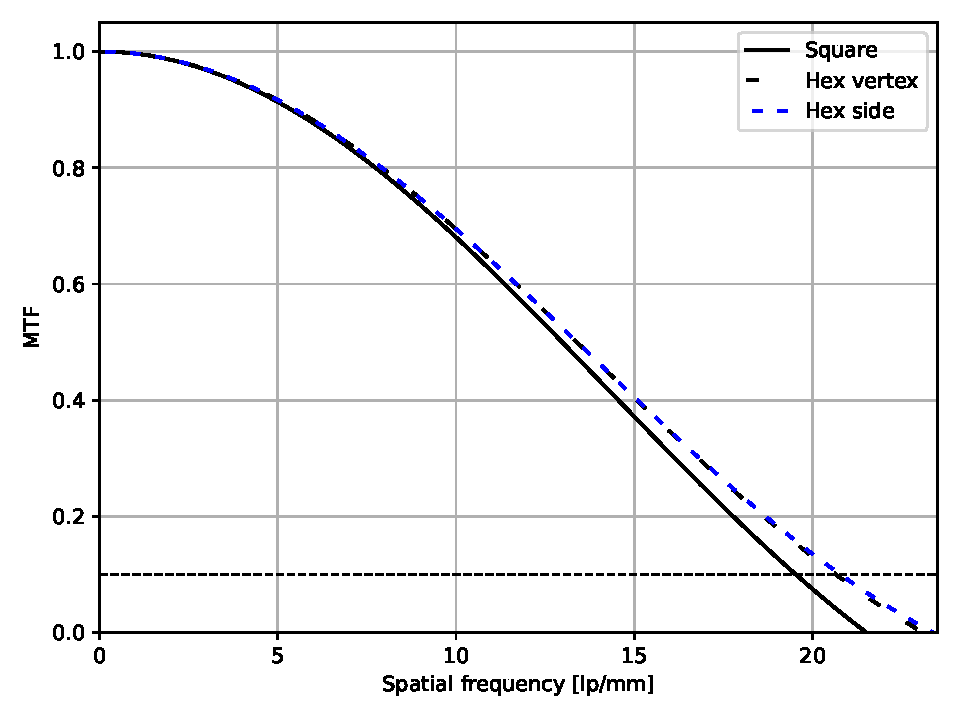
\includegraphics[width=0.6\linewidth]{figures/chapter4/position/mtf_hex_square}
    \caption{MTFs calculated for square and hexagonal pixels with same area. The hexagonal pixel pitch is $p = 50$ $\mu$m. The MTFs referred to the hexagonal pixel are calculated along the directions towards the vertex and orthogonal to the side.}
    \label{fig:mtf_pixels}
\end{figure}

Fig. \ref{fig:mtf_pixels} shows the comparison between the MTF of a square pixel and that of an hexagonal pixel with the same area. It is possible to see that the hexagonal geometry has a slightly better resolution than the square. This can be related to the highest degree of isotropy and symmetry of an hexagon with respect to a square.

Even if no noise sources have been considered for this estimate, it can be interpreted as a lower limit on the resolution of ASIX, as sub-pixel reconstruction algorithms using charge-sharing and diffusion models enable to improve the detector performance.

An alternative and faster way to estimate the spatial resolution of a detector consists of using a line pair phantom, which is a plate with multiple sets of slits with different widths and spatial frequencies, which are expressed as line pair or cycles per millimeter (lp/mm or cycles/mm). The phantom is made of an high-$Z$ material, usually lead. The resolution can be inferred from an image of the phantom by looking at which set of slits is the smallest that can be resolved. The only requirement to use this method is to have a set of slits with a frequency smaller or comparable to the spatial resolution of the detector, but this may not be possible for high resolution detectors.


\begin{figure}[!t]
    \centering
    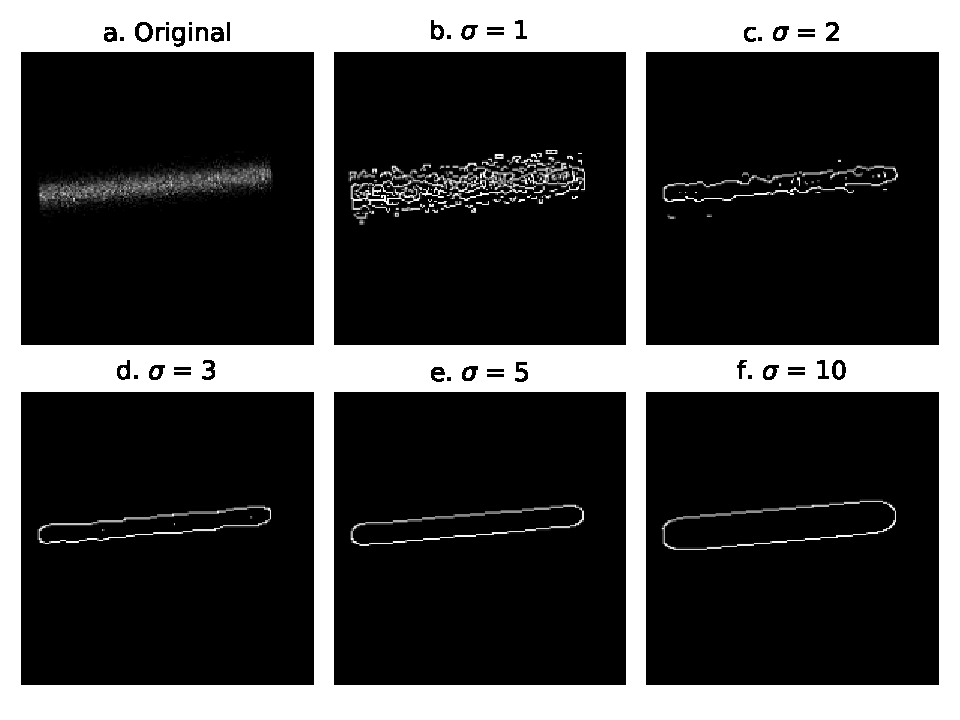
\includegraphics[width=0.8\linewidth]{figures/chapter4/position/mtf_canny}
    \caption{Example usage of the Canny edge detection algorithm on a simulated slit image. The simulated image (a) is binned with a $200 \times 200$ grid, while the slit has a Gaussian profile with a standard deviation of 5 pixels, a length of 160 pixels and a tilt angle of 5 degrees. Images from (b) to (f) show how the detected edges vary by changing the Gaussian filter width. A filter to small is very sensitive to low statistics and detects false edges. Increasing the filter width, this effect becomes less and less visible. If the filter is too wide with respect to the slit width, no edge is detected (case not shown).}
    \label{fig:mtf_canny}
\end{figure}

When using a tilted slit or edge to calculate the MTF, it is necessary to calculate the tilt angle to correctly project the LSF or ESF profile. The procedure to realign the image is described in the case of a slit, but it is the same for an edge.

The angle is determined by the inclination of the slit with respect to the detector $x$-axis. The first step consists of detecting the slit edges in the image. This can be performed using the Canny edge detection algorithm \cite{canny1986}. This algorithm allows to detect the edges in an image and returns a binary image of the same size where a value of 1 means that a pixel is an edge and 0 if it is not.

Before using this algorithm it is necessary to create an image by binning the reconstructed positions. The bin size can not be too large, otherwise the shape and orientation of the slit would be distorted. Another parameter to choose is the width of the Gaussian filter applied by the algorithm to smooth the image. This parameter can not be to small with respect to the slit width, otherwise quantization noise would lead to the detection of false edges. The ideal value should be of the order of the slit width. An example of how the filter width affects edge detection is shown in Fig. \ref{fig:mtf_canny}.

The second step of the process consists of calculating the angle from the detected edges, which are sets of straight lines. This can be performed with the use of the Hough transform \cite{hough1959, duda1972}, which is a technique used to detect parameterizable curves, such as lines.

A line in the plane is represented by a set of two parameters $(\rho, \theta)$, which define the Hough space, where $\rho$ is the distance of the line from the origin of the axes and $\theta$ is the angle between the $x$-axis and the distance vector. Within this representation, each point $(x, y)$ on a straight line is described by

\begin{equation}
\rho = x \cos \theta + y \sin \theta.
\label{eq:hough}
\end{equation}

\begin{figure}[!t]
    \centering
    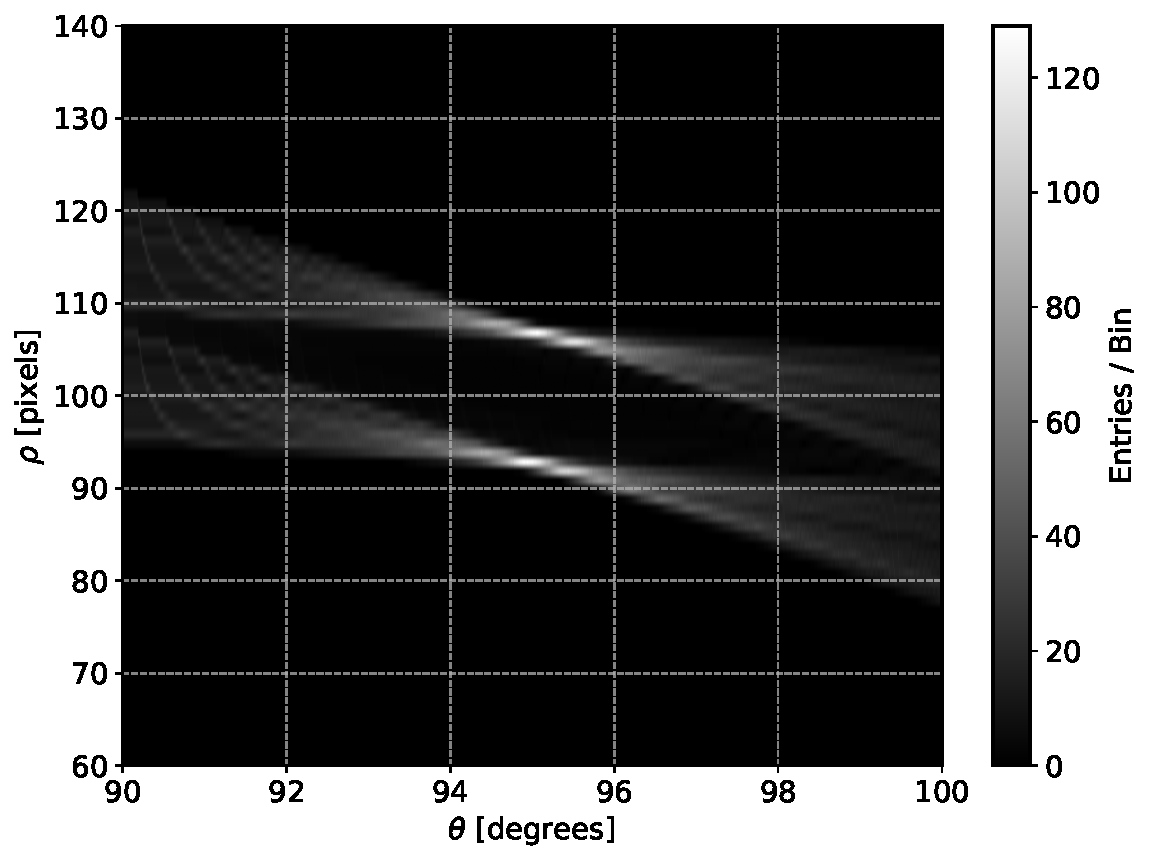
\includegraphics[width=0.7\linewidth]{figures/chapter4/position/mtf_hough}
    \caption{Accumulator space resulting from the Hough transform of the slit edge image from Fig. \ref{fig:mtf_canny}(e). The two nearly identical peaks that are visible correspond to the two long edges of the slit.}
    \label{fig:mtf_hough}
\end{figure}

For each point of the edges, the algorithm scans a given range of $\theta$ values and for each one evaluates Eq. \ref{eq:hough}. The results are accumulated in a two-dimensional histogram, named accumulator space, where for each point and angle value an entry is added at the correspondent bin $(\rho, \theta)$. A straight line is detected when a peak is identified in the latter space, and the tilt angle can be calculated as $\theta_{peak} - \pi/2$. An example of the result of the Hough transform of the edges of a  slit is shown in Fig. \ref{fig:mtf_hough}. During the analysis, if multiple lines are present and multiple peaks are produced by the Hough transform, only the highest one is considered to calculate the tilt angle.

To calculate the presampled LSF, the slit image has to be rotated by the angle found with the Hough transform. Once it has been aligned, the presampled LSF is calculated projecting all the points on the short side of the slit and calculating the histogram of the reconstructed positions. The bin size of this histogram must be smaller than the expected resolution of the detector, in order to not incur in aliasing effects, as stated by the Nyquist theorem, but large enough to not be sensitive to noise.

A possible way to limit distortions from noise is to apply a smoothing algorithm on the LSF, but remembering that in frequency domain a smoothing acts as a low-pass filter, with the possible consequence of underestimating the actual detector resolution.

The presampled MTF is then calculated from the LSF using a discrete fast Fourier transform algorithm. The LSF and MTF calculated from the previous examples are shown in Fig. \ref{fig:slit_lsf_mtf}.

In conclusion, the MTF currently represents the only available way to characterize the spatial resolution of the ASIX prototypes, and this analysis can be performed both on real and simulated data, in order to verify the consistency between the difference of the various implemented reconstruction algorithm and also the consistency between data and simulations.

\begin{figure}[h]
    \centering
    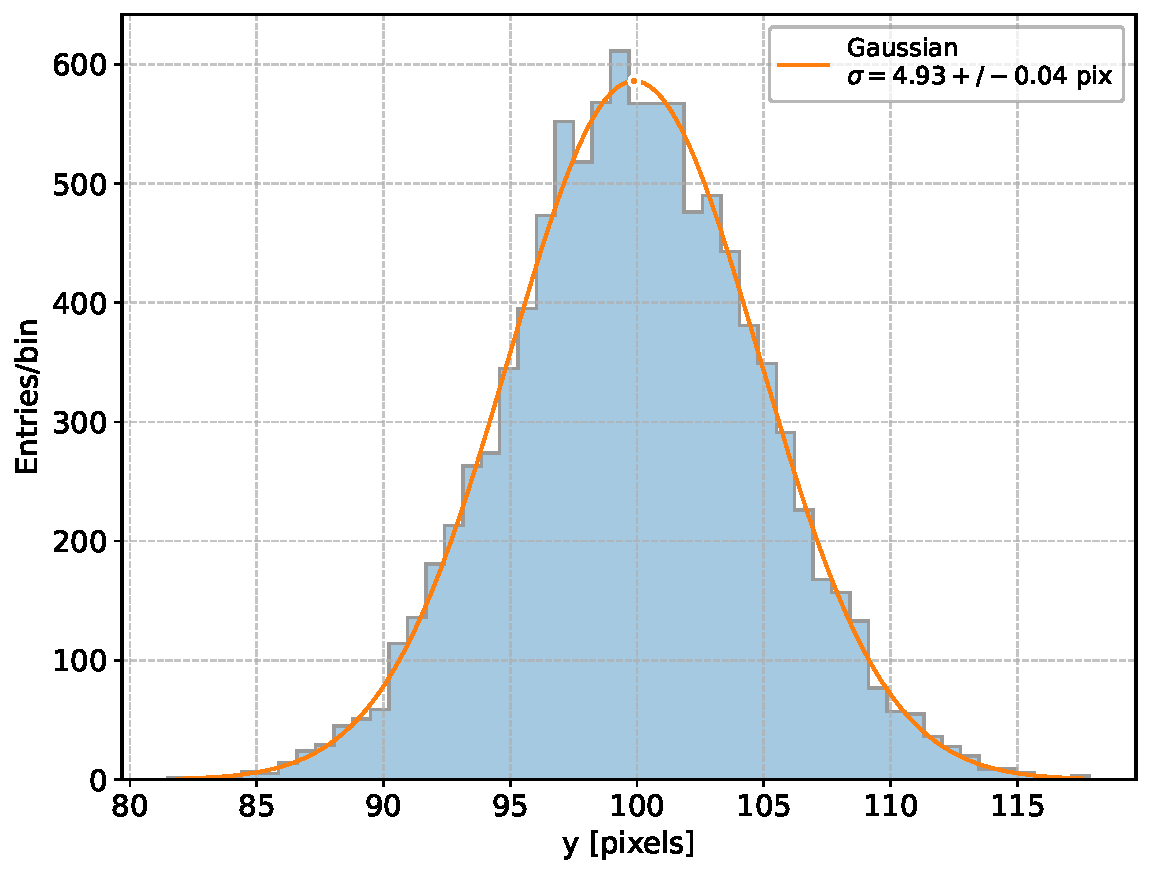
\includegraphics[width=0.49\linewidth]{figures/chapter4/position/mtf_lsf}
	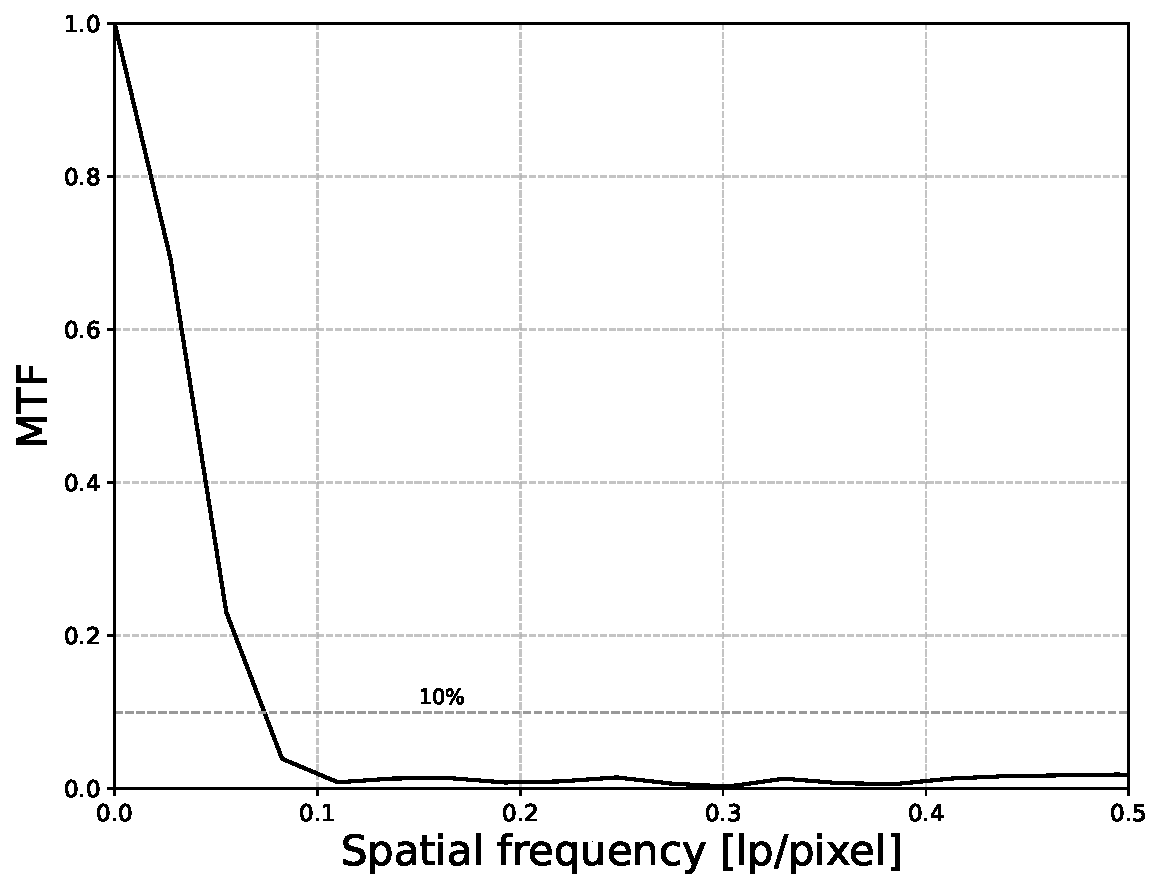
\includegraphics[width=0.49\linewidth]{figures/chapter4/position/mtf}
    \caption{Line spread function (left panel) and modulation transfer function (right panel) calculated for the slit using the edges from Fig. \ref{fig:mtf_canny}(e) and the tilt angle from \ref{fig:mtf_hough}. The slit was simulated with a Gaussian profile with $\sigma = 5$ pix. The standard deviation estimated from an LSF fit is $\sigma_{\textrm{fit}} = 4.93 \pm 0.04$ pix, while from the MTF is $\sigma_{\operatorname{MTF}} = 4.7$ pix using Eq. \ref{eq:mtf_sigma}.}
    \label{fig:slit_lsf_mtf}
\end{figure}


\section{Energy reconstruction}
Using the calibration products it is possible to estimate the photon energy for each event and calculating the spectrum of a source. If the absolute gain has been calibrated, the spectrum can be expressed in terms of eV instead of ADC counts if only the normalized gain has been calibrated. However, the difference is only a scale factor, thus it is not relevant.

As for position reconstruction, there are different algorithms that can be employed in the energy reconstruction. Specifically, two algorithms have been developed and will be explained in this section.

The performances of these algorithms will be shown in Chap. \ref{sec:results}, where laboratory data will be analyzed and the results are compared to simulations. The metric to determine the goodness of these algorithms is the FWHM of a given spectral line.

\subsection{Suppression algorithm}
The first energy reconstruction method is based on the suppression algorithm described in Chap. \ref{sec:analysis}. This algorithm consists of suppressing some of the pixels in an event by using a charge and a geometrical constraint, in order to minimize the probability of including pixels with charge not produced by the photon.

The charge constraint consists of selecting a threshold value, expressed in terms of noise $\sigma$ for each pixel. If a pixel has an amount of charge smaller than the threshold it is suppressed, thus its charge is put to zero. The geometrical constraint follows from the charge diffusion model and it consists of requiring that all the pixels that are above the threshold are adjacent. Furthermore, given the small charge diffusion width, if more than three pixels are above threshold only the three adjacent pixels with the most charge are kept.

This is the same algorithm that is employed to determine an event cluster size and that is applied before position reconstruction when using charge barycentering and $\eta$ algorithms.

After suppressing the pixels, the photon energy is calculated by summing the charge collected by all the unsuppressed pixels.

This method has a free parameter that can be varied, which is the value of the zero-suppression threshold. The final energy resolution depends on this parameter, and it is important to find the best value. This dependence will be shown on laboratory data in the next section.

\subsection{Likelihood estimator}
The second method to estimate the photon energy is to use the likelihood estimator introduced in Chap. \ref{subsec:mle} for the position reconstruction. The likelihood that describes the charge diffusion depends both on the photon incident position and energy, as shown in  Eq. \ref{eq:nll_multivariate}.

This algorithm has been already explained in detail in the previous section, and contrary to the suppression method it does not require an arbitrary threshold. Indeed, the likelihood model intrinsically weights the pixel charges through a simultaneous minimization of both the incident position and the photon energy.

\section{Results}
\label{sec:results}
The detector's imaging and energy resolutions are directly determined by the performance of the position and energy reconstruction methods. To accurately assess these properties, specific datasets were employed for each task.

These datasets were collected in the laboratory using ASIX prototypes. As previously mentioned, the current prototypes are equipped with the XPOL-III ASIC, which differs from the final design in several aspects. The most significant difference is the electronic noise, which is currently four to five times higher than the design goal.

\begin{figure}[!b]
    \centering
    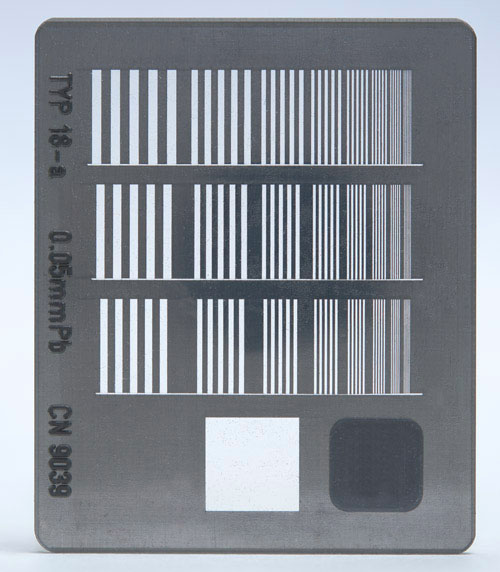
\includegraphics[width=0.4\linewidth]{figures/chapter4/results/huttner}
	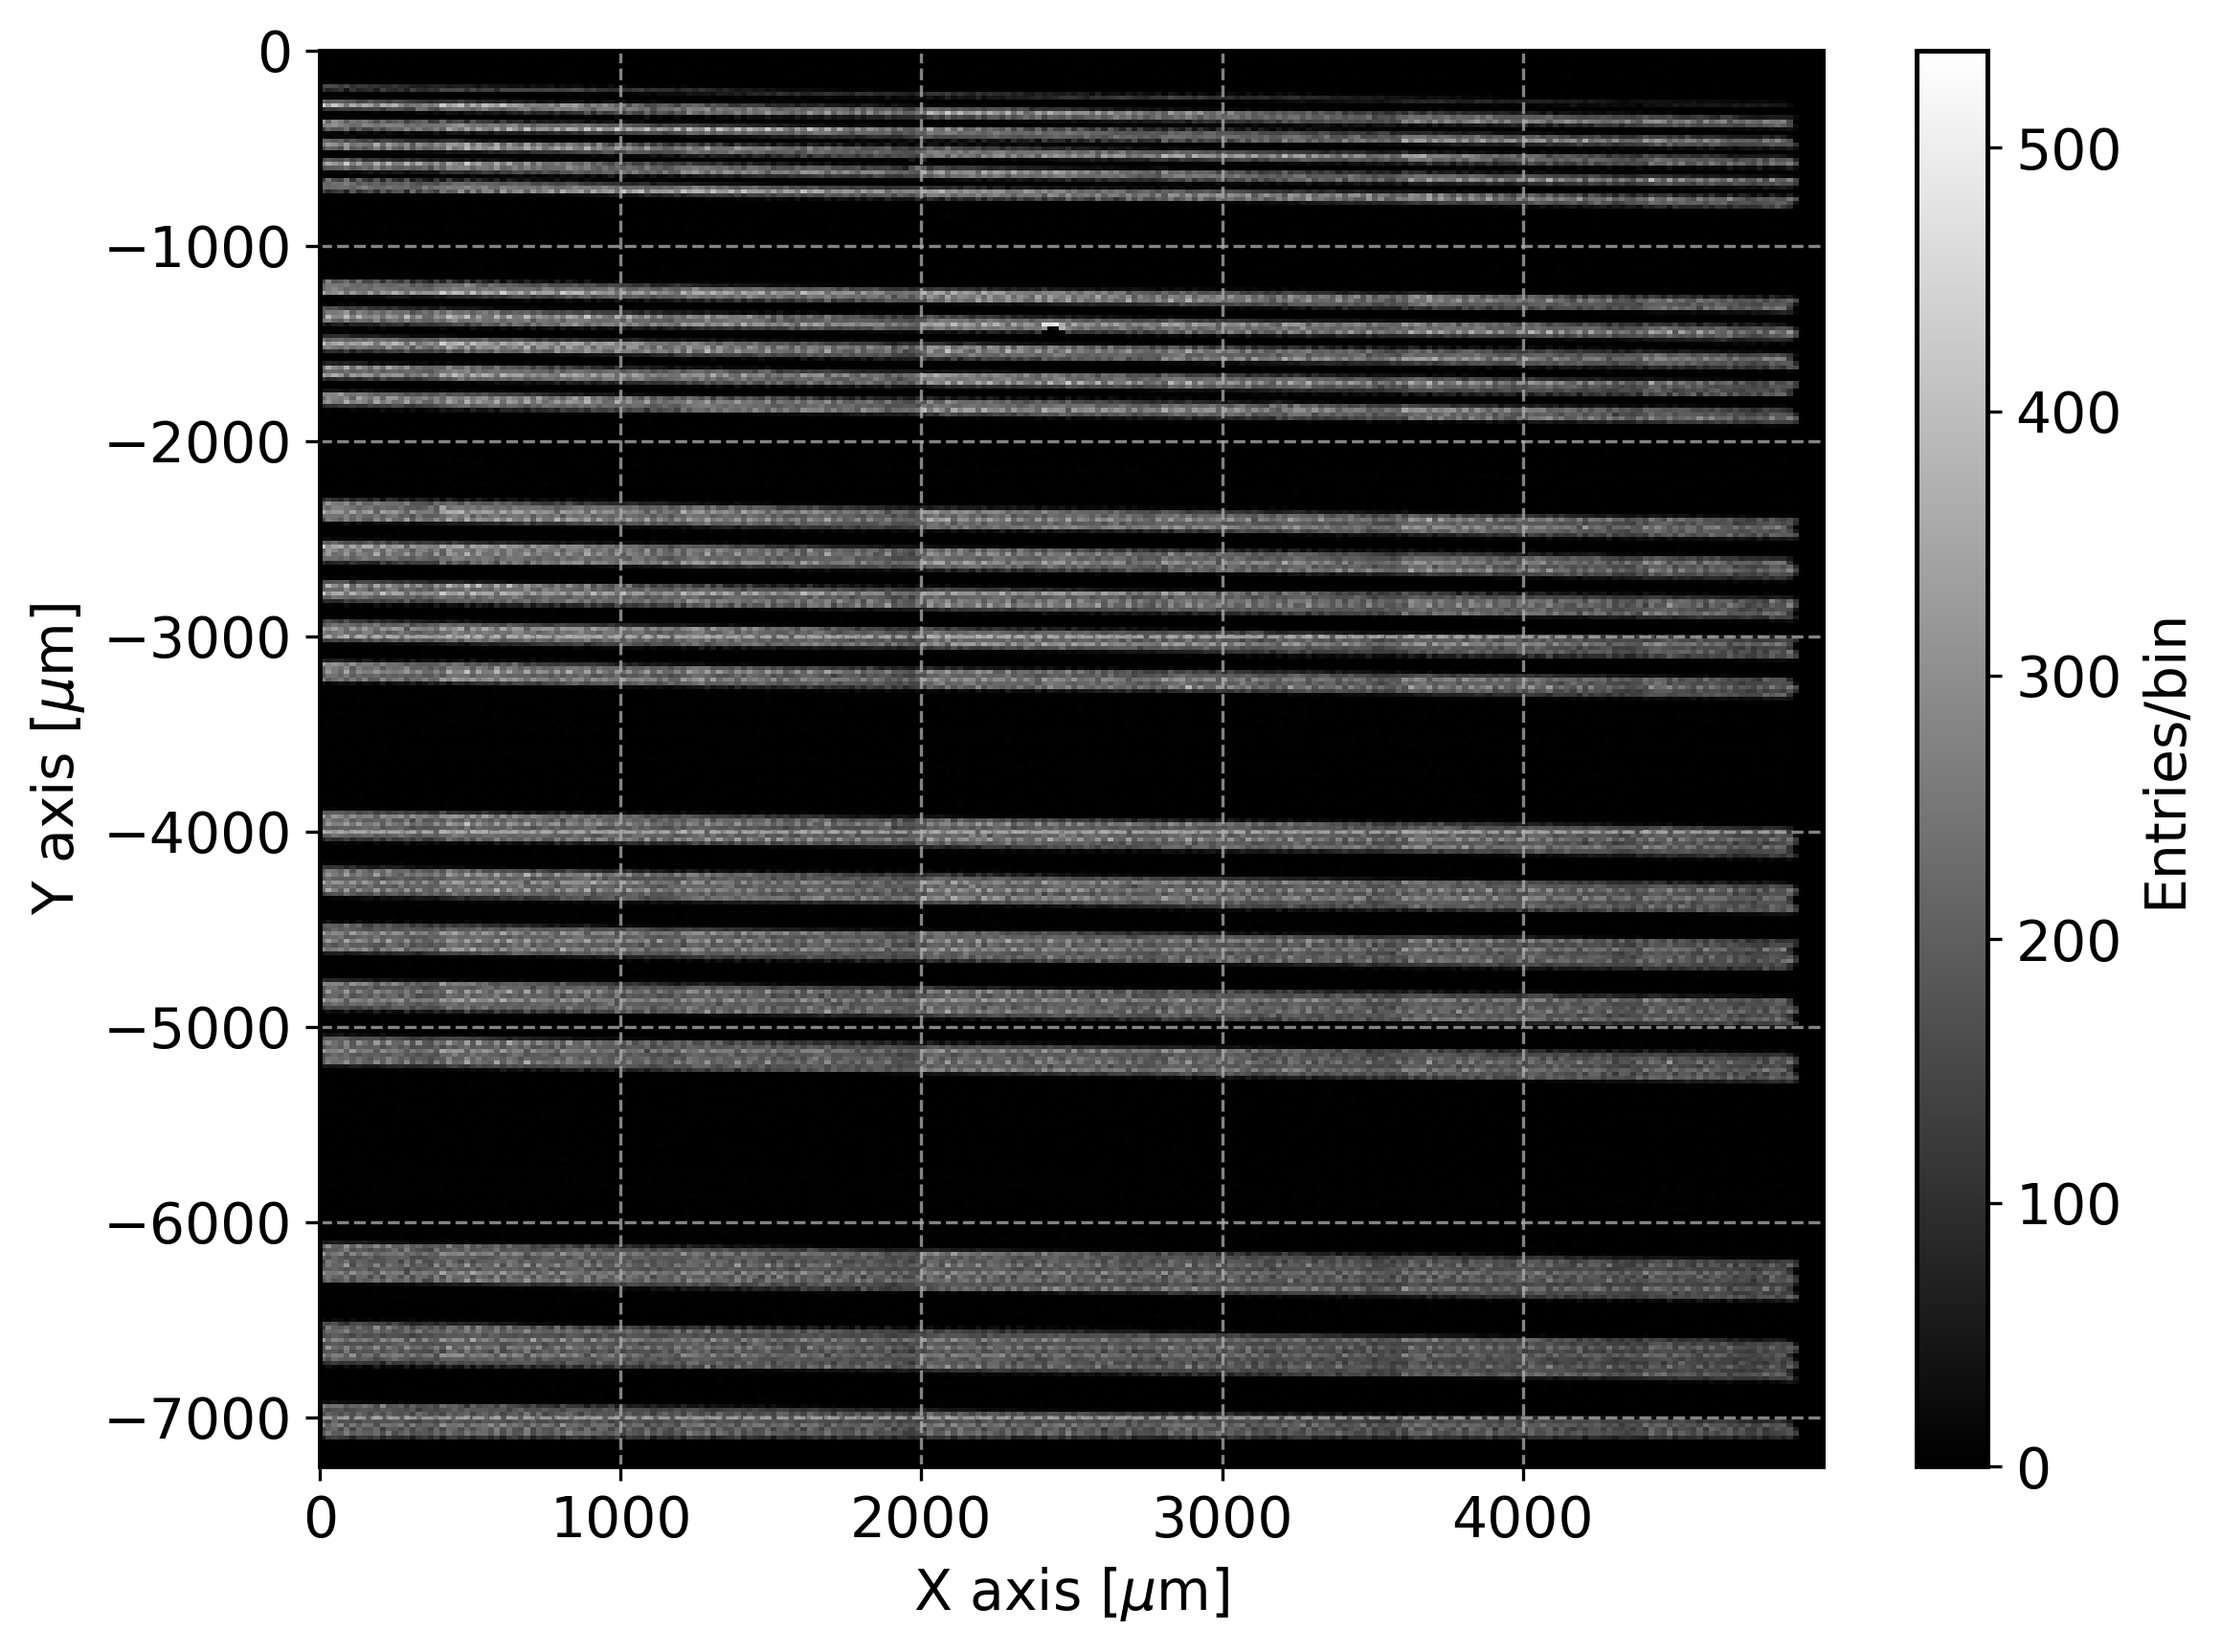
\includegraphics[width=0.59\linewidth]{figures/chapter4/results/slits_hist}
    \caption{The left panel shows an example of Huttner phantom similar to the one employed in the experimental setup. The right panel shows the phantom reconstructed image using the centroid algorithm. It is possible to observe differnent slit sets with various frequencies.}
    \label{fig:huttner}
\end{figure}

Reducing this noise is precisely the major improvement of the final design, which will allow the achievement of very high resolutions in both imaging and spectroscopy. In the current setup, in fact, the total noise is largely dominated by the electronics. However, even in this high-noise regime, the collected data allow us to verify the effectiveness of the developed algorithms and to study how the choice of the method affects the final resolution.

Additionally, these datasets provide a crucial opportunity to validate the Monte Carlo simulations against real data. Accurate simulations are not only important to understand the intrinsic limits of the detector based on its physical properties, but they are also strictly required for the calibration of some of the reconstruction methods.

In this section, the experimental setups used to collect the data for the imaging and spectral resolution estimation are described. Furthermore, dedicated Monte Carlo simulations matching these setups are presented. These simulations are used to calibrate the different reconstruction algorithms and to provide a baseline for comparing the final resolution results.

 
\subsection{Spatial resolution}
To estimate the detector spatial resolution a Huttner phantom similar to the one shown in Fig. \ref{fig:huttner} has been used. The phantom is made of a 50 $\mu$m thick lead slab with multiple sets of slits with different spatial frequencies, ranging from a minimum of 0.5 lp/mm up to a maximum of 10 lp/mm.

\begin{figure}[!b]
    \centering
    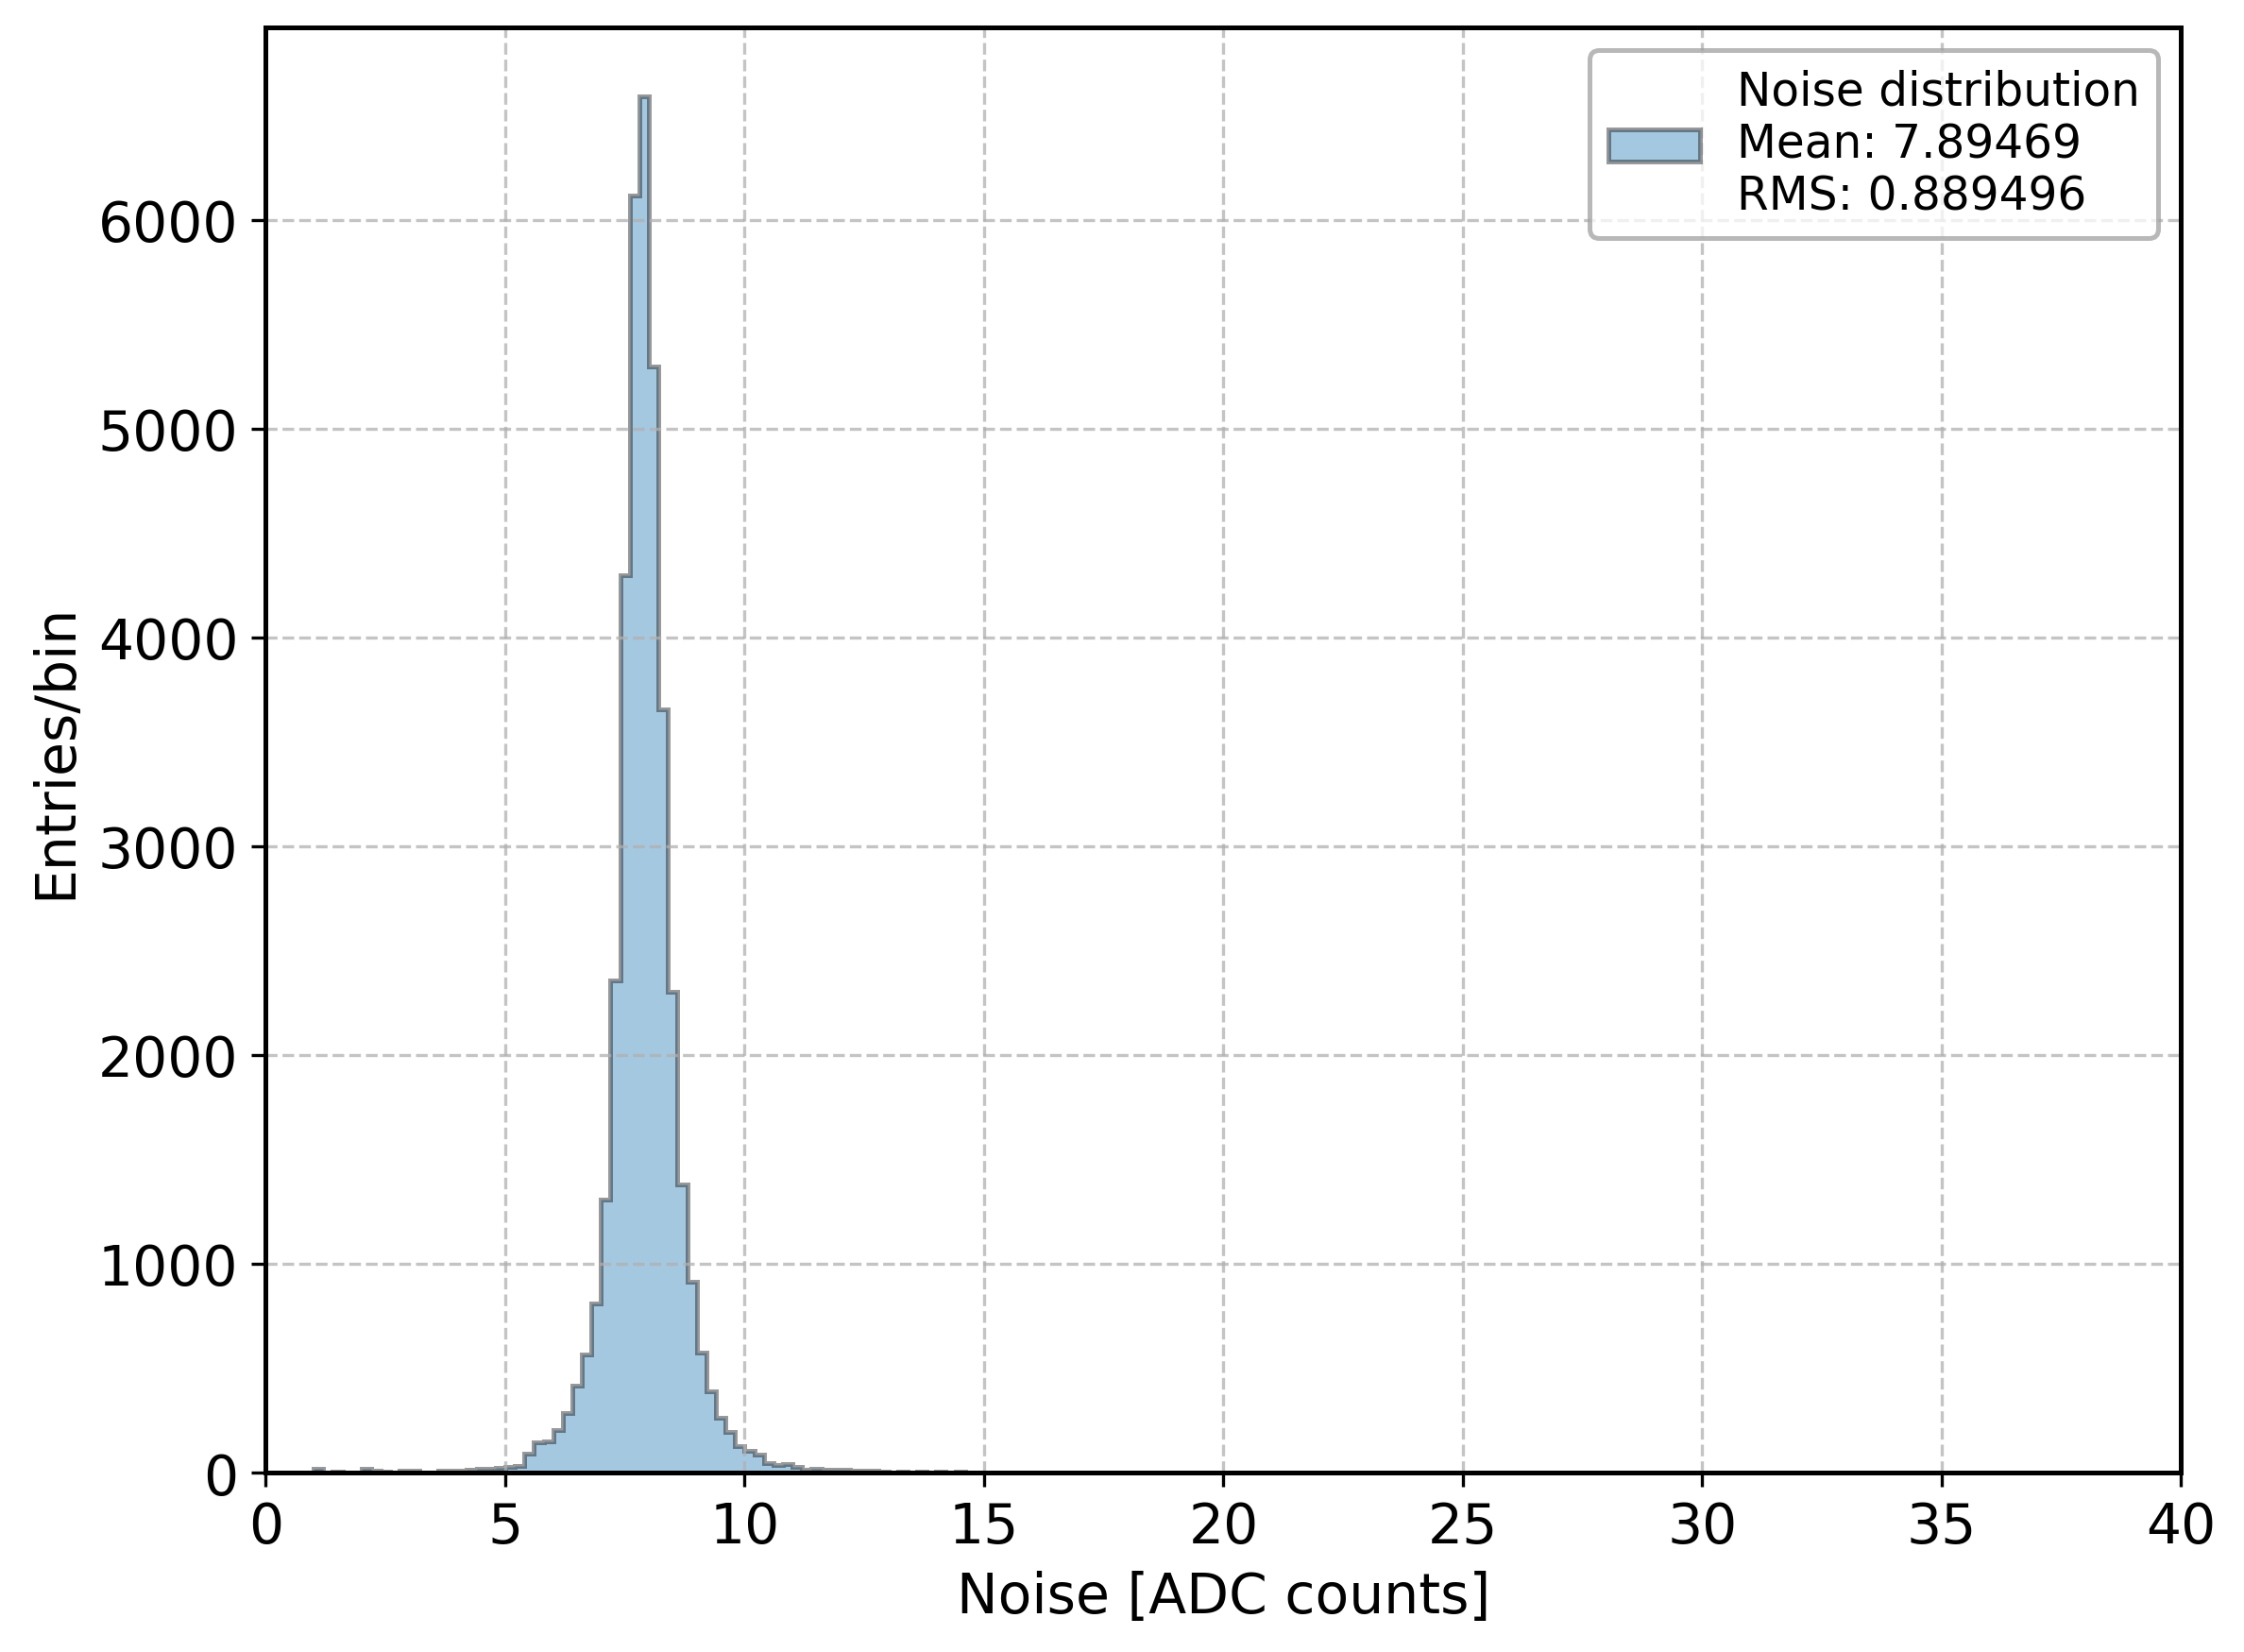
\includegraphics[width=0.49\linewidth]{figures/chapter4/results/noise_hist}
	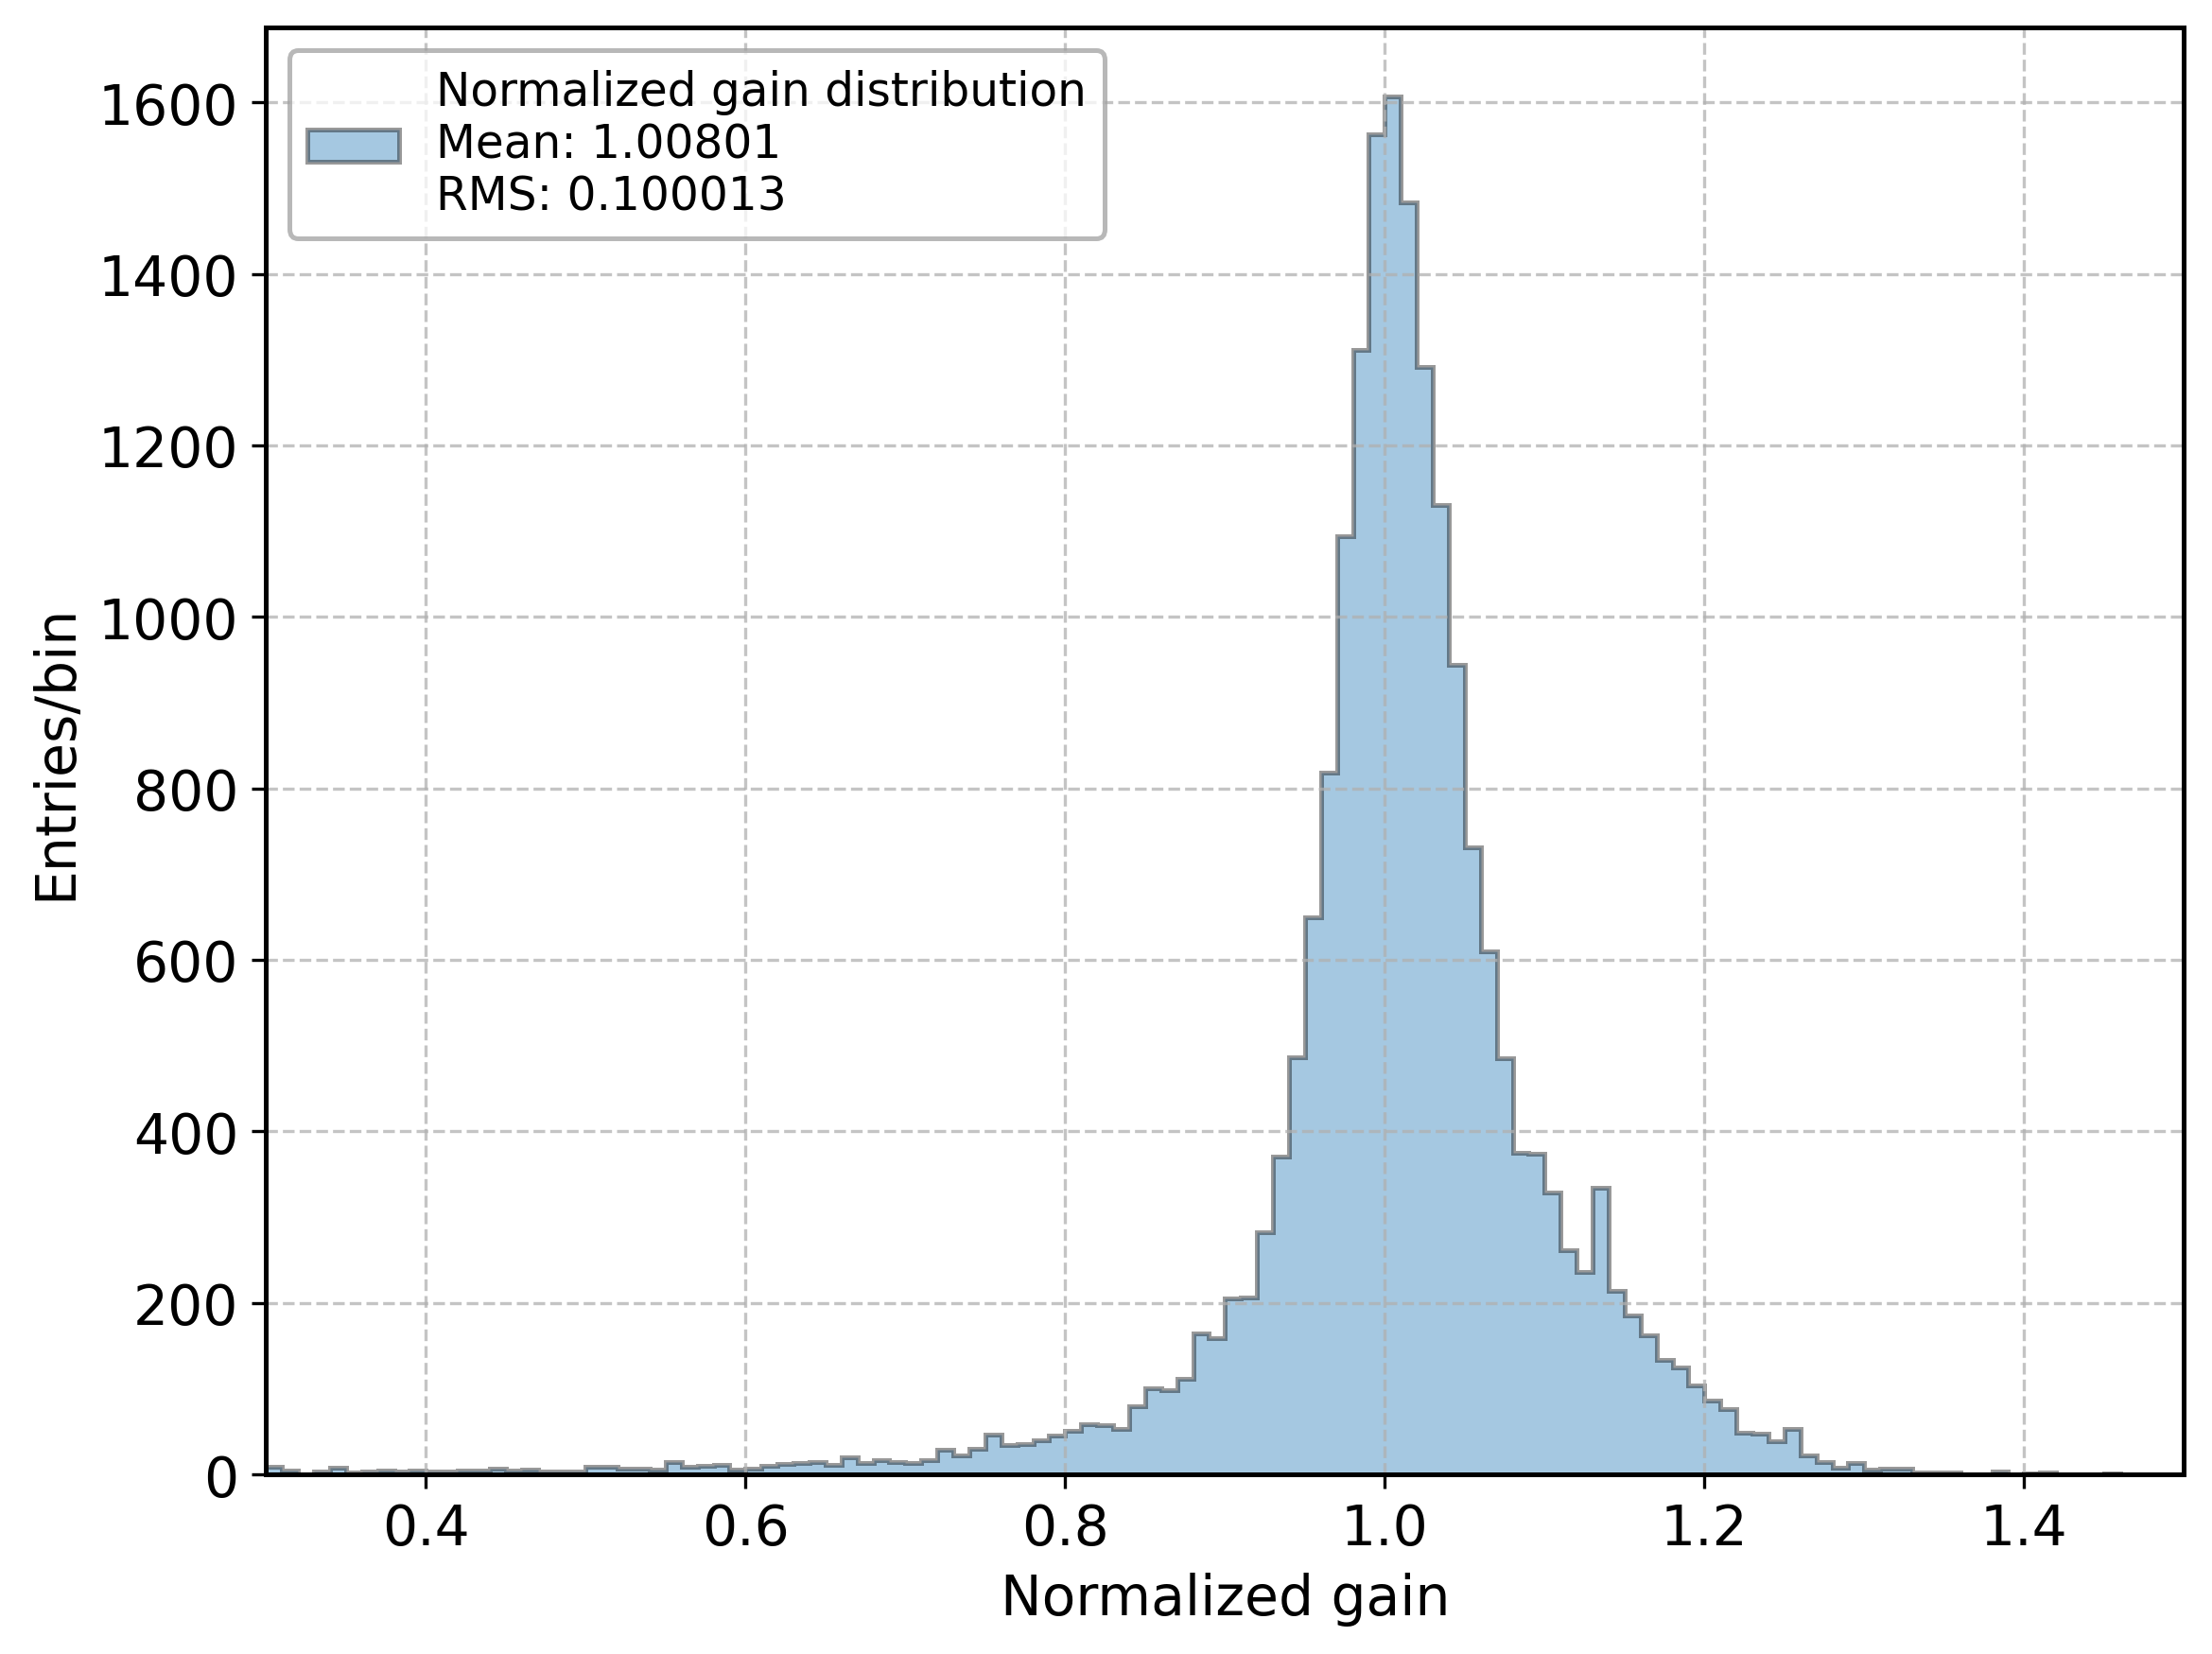
\includegraphics[width=0.49\linewidth]{figures/chapter4/results/equalization_hist}
    \caption{Calibration products obtained from the Huttner phantom laboratory data set. The noise distribution (left panel) has a mean of about 8 ADC counts and a standard deviation of 0.9 ADC counts. The normalized gain has a variation of 10\%.}
    \label{fig:results_cal}
\end{figure}

The phantom portion with the highest frequencies is placed above the detector and it is irradiated with X-rays generated by an X-ray tube which is operated at 10 kV with a gold target \cite{minuti2025}. The X-ray tube is located 1 m from the phantom, in order to have a collimated photon beam. Operating the tube at a voltage of 10 kV with a gold target is not enough to observe fluorescence lines, thus the resulting spectrum is mainly due to Bremsstrahlung emission from accelerated electrons. 

The tested prototype is the one with the silicon sensor, which have pixels with 50 $\mu$m pitch. Given that the expected resolution is smaller than the pixel pitch, the available Hutnner phantom does not have a frequency large enough to be used for a visual estimate of the resolution. The solution is to use the edge of a large slit to calculate the ESF, from which the MTF can then be calculated.

Before the event reconstruction, the detector calibration is performed to estimate the noise level of the pixels. Given that for XPOL-III the pedestal subtraction is performed directly on the chip, the first noise calibration method described in Chap. \ref{sec:calibration} is adopted. Then, the normalized pixel gain is calibrated. The noise and normalized gain distributions are shown in Fig. \ref{fig:results_cal}.

\begin{table}[!t]
\centering
\begin{tabularx}{\textwidth}{X cc}
Reconstruction Algorithm & $f_{10}$ Lab. data [lp/mm] & $f_{10}$ Sim. data [lp/mm]\\
\midrule
Charge barycentering & 47.1 & 53.9 \\
MLE                  & 51.7 & 68.0 \\
Unmodeled $\eta$     & 51.9 & 71.0 \\
Modeled $\eta$       & 51.7 & 67.4 \\
\bottomrule
\end{tabularx}
\caption{Values $f_{10}$ for which $\operatorname{MTF}(f_{10}) = 0.1$ for different reconstruction algorithm calculated for laboratory data and simulated data.}
\label{tab:results_mtf}
\end{table}

\begin{figure}[!b]
    \centering
    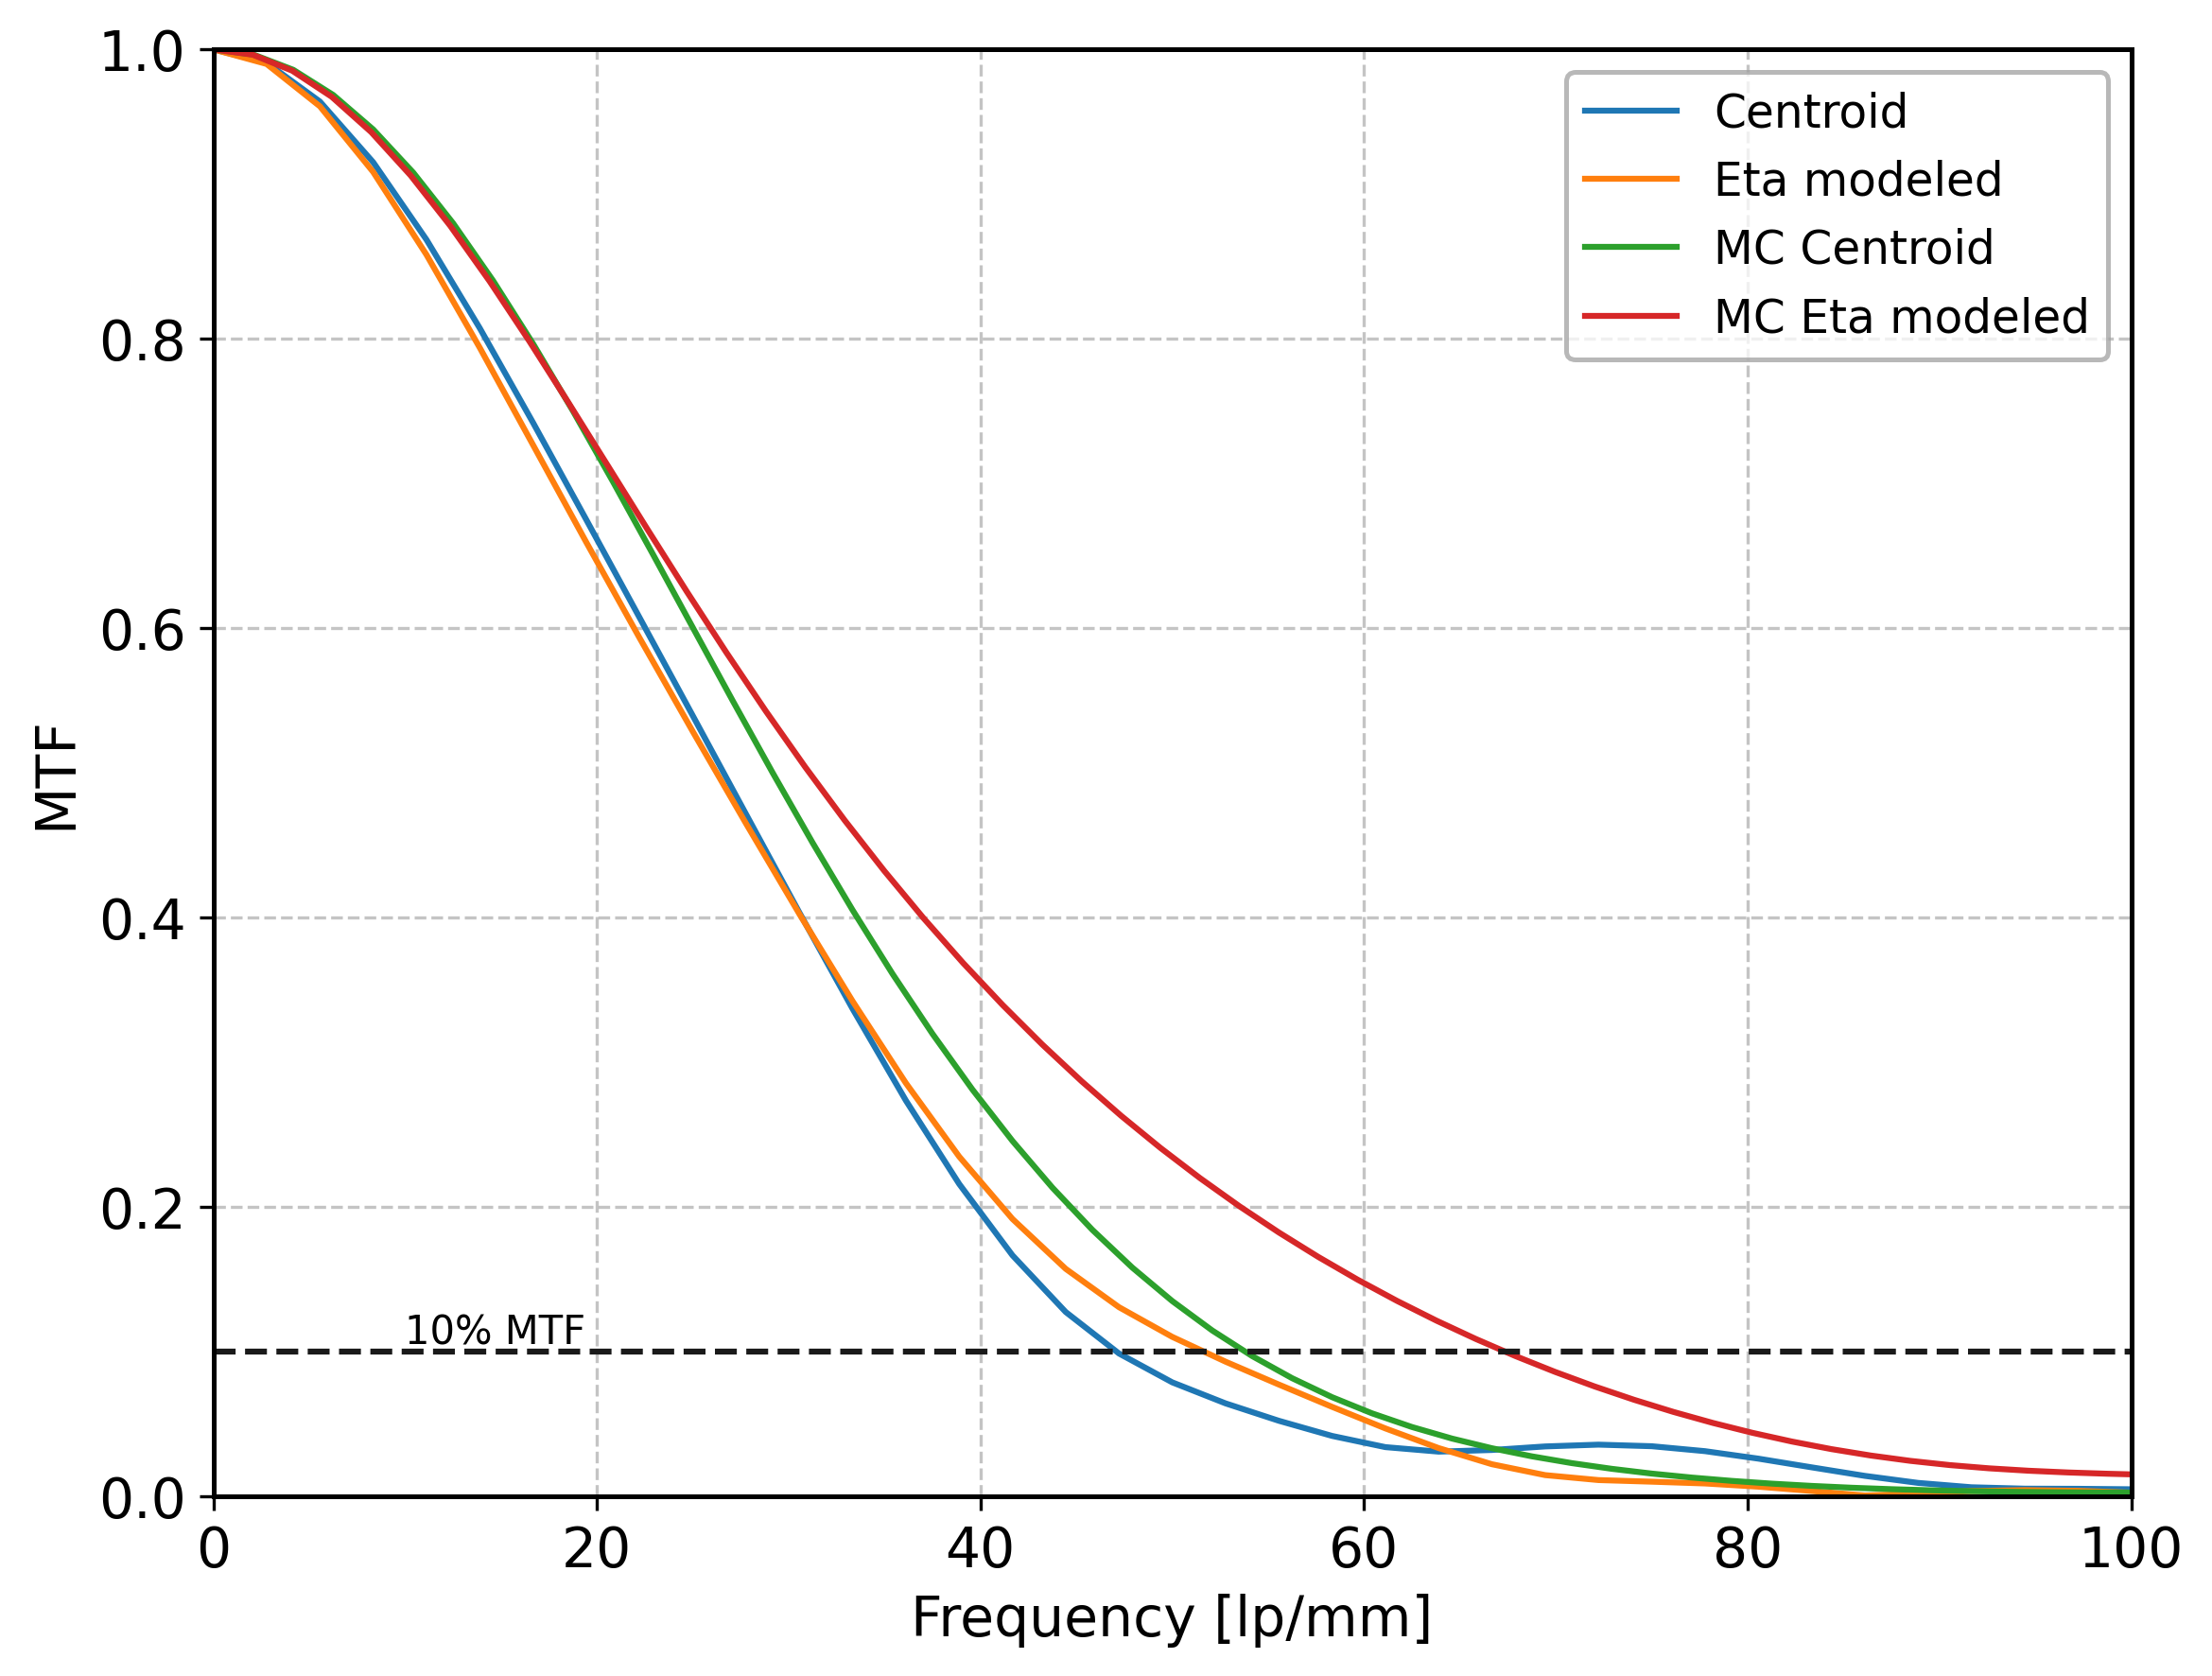
\includegraphics[width=0.7\linewidth]{figures/chapter4/results/slits_mtf}
    \caption{Modulation transfer function obtained with different reconstruction methods for laboratory data and simulated data. Solid lines represent MTF calculated from laboratory data. Dashed lines represent MTF calculated from simulated data}
    \label{fig:results_mtf}
\end{figure}


Once the noise and gain of the detector are characterized, a simulated dataset with matching noise, gain and spectrum shape is generated to calibrate the reconstruction methods. After that, the laboratory data can be analyzed and the event positions can be estimated with the different algorithms. The resulting positions are shown in Fig. \ref{fig:huttner} and it is possible to observe the distribution of the positions along the phantom slits. To estimate the spatial resolution, the method described in Chap. \ref{subsec:mtf} to align and project the reconstructed positions along the axis perpendicular to the slanted slit is used to calculate the MTF.

A new Monte Carlo data set with a slit of the same size of the one analyzed in the laboratory data is simulated to compare the obtained results with those expected from simulations. The data set is generated using the same distribution of noise and normalized gain. After the data set is generated, it is analyzed with the same method used for laboratory data. The MTFs obtained with the different algorithms for laboratory data and simulated data are shown in Fig. \ref{fig:results_mtf} and the values $f_{10}$ for which MTF is 10\% are reported in Tab. \ref{tab:results_mtf}. 

From the analysis of laboratory data, the improvement in the spatial resolution obtained using more complex algorithms than charge barycentering is not as big as expected. Indeed, from Monte Carlo simulations the resolution achieved with the best algorithm, the $\eta$ unmodeled, is about 30\% better than charge barycentering. This behavior can be associated to different factors. An example is the possibility of having defects in the Huttner phantom slit edges. Indeed, the Huttner phantom is designed to have a quick estimate of the resolution and is not ideal to carry on a detailed analysis with the slanted edge. These defects can transmit unwanted photons, thus producing a degraded edge image.

\subsection{Energy resolution}
To estimate the energy resolution, a different experimental setup has been employed. For this purpose it is essential to produce a known spectrum with separated lines. To test the ASIX silicon prototype a gold target has been irradiated by an X-ray tube operated at 25 kV, in order to produce fluorescence lines.

To suppress the Bremsstrahlung continuum spectrum and only detect fluorescence lines, the gold target is tilted with respect to the X-ray tube and only the fluorescence radiation, which is emitted isotropically, reaches the detector. The experimental setup is shown in Fig. \ref{fig:spectral_setup}. With this setup the beam is very small and collimated and it illuminates only an area of about 50 pixels. The observed spectrum shows fluorescence lines produced by $L$-shell transitions. In particular the dominant lines are the $L\alpha$ doublet at about 9.7 keV, the $L\beta$ doublet at 11.5 keV and the $L\gamma$ triplet at 13.4--13.8 keV.

\begin{figure}[htbp]
  \centering
  \begin{tikzpicture}[>=LaTeX, font=\sffamily]

    % Colori
    \definecolor{tubeBody}{RGB}{240, 240, 240}
    \definecolor{goldColor}{RGB}{245, 195, 35}
    \definecolor{detectorColor}{RGB}{235, 235, 235}
    \definecolor{xrayPrimary}{RGB}{210, 40, 40}
    \definecolor{xrayFluo}{RGB}{30, 110, 220}

    % 1. TUBO A RAGGI X ORIZZONTALE (A sinistra)
    \begin{scope}[shift={(-4.2, 0)}]
      % Struttura esterna
      \draw[thick, fill=tubeBody, rounded corners=3pt] (-1.5, -0.6) rectangle (1.5, 0.6);
      % Anodo interno
      \draw[thick, fill=gray!50] (0.8, -0.4) -- (1.1, -0.4) -- (0.7, 0.4) -- (0.4, 0.4) -- cycle;
      % Filamento / Catodo
      \draw[very thick, gray!80] (-1.0, -0.25) -- (-1.0, 0.25);
      \draw[thick, gray!80] (-1.0, 0) -- (-0.4, 0);
      % Finestra di uscita
      \draw[thick, fill=white] (1.5, -0.3) rectangle (1.6, 0.3);
      \node[above, font=\sffamily\small] at (0, 0.65) {X-ray tube};
    \end{scope}

    \coordinate (Source) at (-2.6, 0);

    % 2. TARGET: FOGLIO D'ORO INCLINATO A -45° (Centro in (0,0))
    \coordinate (Target) at (0, 0);

    \begin{scope}[rotate around={-45:(Target)}]
      \draw[thick, fill=goldColor] (-1.2, -0.09) rectangle (1.2, 0.09);
    \end{scope}

    \node[right, font=\sffamily\small, align=left] at (0.8, 0.8) {Au target};
    \draw[->, thick, gray!80] (0.8, 0.6) -- (0.25, 0.25);

    % 3. FASCIO PRIMARIO ORIZZONTALE (Incide al centro della foglia in (0,0))
    \draw[ultra thick, xrayPrimary, ->] (Source) -- (Target) 
      node[midway, above, font=\sffamily\small\bfseries, text=xrayPrimary] {};

    % 4. DETECTOR (Centrato rispetto a (0,0), parallelo al pavimento)
    \coordinate (DetCenter) at (0, -2.5);
    \draw[thick, fill=detectorColor] (-1.3, -2.9) rectangle (1.3, -2.1);
    \node[font=\sffamily\small] at (DetCenter) {Detector};

    % 5. EMISSIONE DI FLUORESCENZA IN RIFLESSIONE (Isotropica)
    % Raggio centrale che va al centro del detector (0, -2.1)
    \draw[thick, xrayFluo, ->] (Target) -- (0, -2.1);
    
    % Raggi laterali verso le estremità del detector
    \draw[thick, xrayFluo, ->] (Target) -- (-0.9, -2.1);
    \draw[thick, xrayFluo, ->] (Target) -- (0.9, -2.1);

    % Frecce tratteggiate esterne (indicatrici dell'emissione isotropica)
    \foreach \angle in {210, 235, 305, 330} {
      \draw[thick, xrayFluo, ->, >=stealth, dashed] (Target) -- (\angle:1.8);
    }

    \node[right, font=\sffamily\small, text=xrayFluo, align=left] at (1.5, -1.2) {Isotropic fluorescence\\radiation};

  \end{tikzpicture}
  \caption{Scheme of the experimental setup for spectral resolution study. The X-ray tube illuminates the Au target which in turn emits fluorescence radiation that irradiates the detector.}
  \label{fig:spectral_setup}
\end{figure}

Before analyzing the data, the detector calibration procedure is performed in order to compensate variations between the pixels. The noise level distribution is approximately a Gaussian with mean around 8 ADC counts and a standard deviation of about 1 ADC counts. The normalized gain is approximately uniform with a standard deviation of 3\%. The obtained calibration products are also used to run a Monte Carlo simulation with the $L\alpha$ and $L\beta$ gold lines and with the same noise and gain distributions of the detector, in order to compare the results between the two datasets.

The energy is then reconstructed using the two methods described in the previous section. When applying the suppression algorithm, different thresholds can be adopted, making it relevant to investigate how the threshold affects the energy resolution. To evaluate the resolution, the $L\alpha$ and $L\beta$ lines are fitted simultaneously using the model described in Eq.~\ref{eq:two_lines_fit}, and the resolution is derived from the FWHM of the $L\alpha$ peak. 

An example of a measured spectrum along with its best-fit curve, as well as the dependence of the energy resolution on the threshold for both experimental and simulated datasets, are shown in Fig.~\ref{fig:spectrum_fit}. While for laboratory data the best energy resolution is achieved at a threshold around 2.5--3.0\,$\sigma$, in the simulations the optimal resolution is obtained with zero threshold. The origin of this discrepancy is not fully understood, but it can likely be attributed to secondary, low-intensity lines present in the experimental gold spectrum that are not modeled in the simulation, as well as pixel-correlated noise sources present in the real setup. Despite this difference, the best energy resolution measured for both datasets, which is 13.5\% (1300 eV) for laboratory data and 12.5\% (1200 eV) for simulated data, does not differ significantly from the expected energy resolution at 9.7 keV of about 11\% (970 eV).

\begin{figure}[!b]
    \centering
    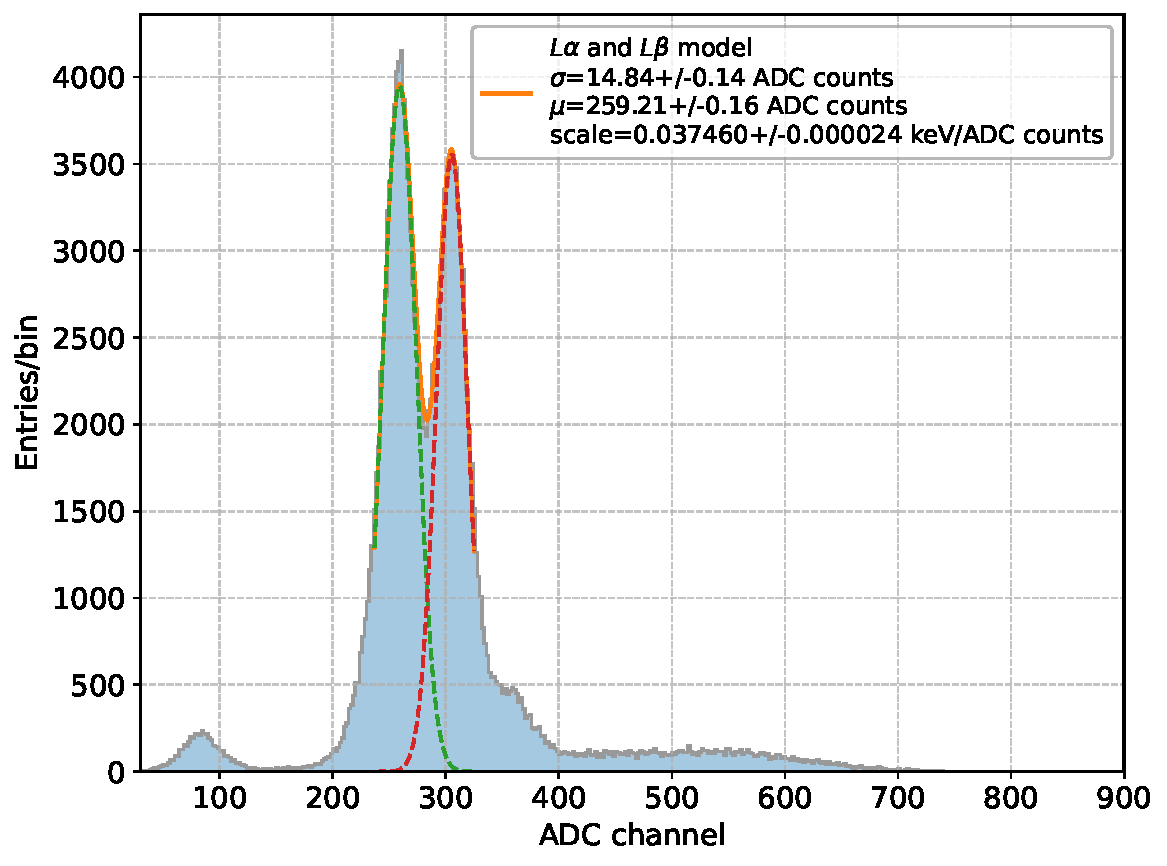
\includegraphics[width=0.49\linewidth]{figures/chapter4/results/spectrum_example}
    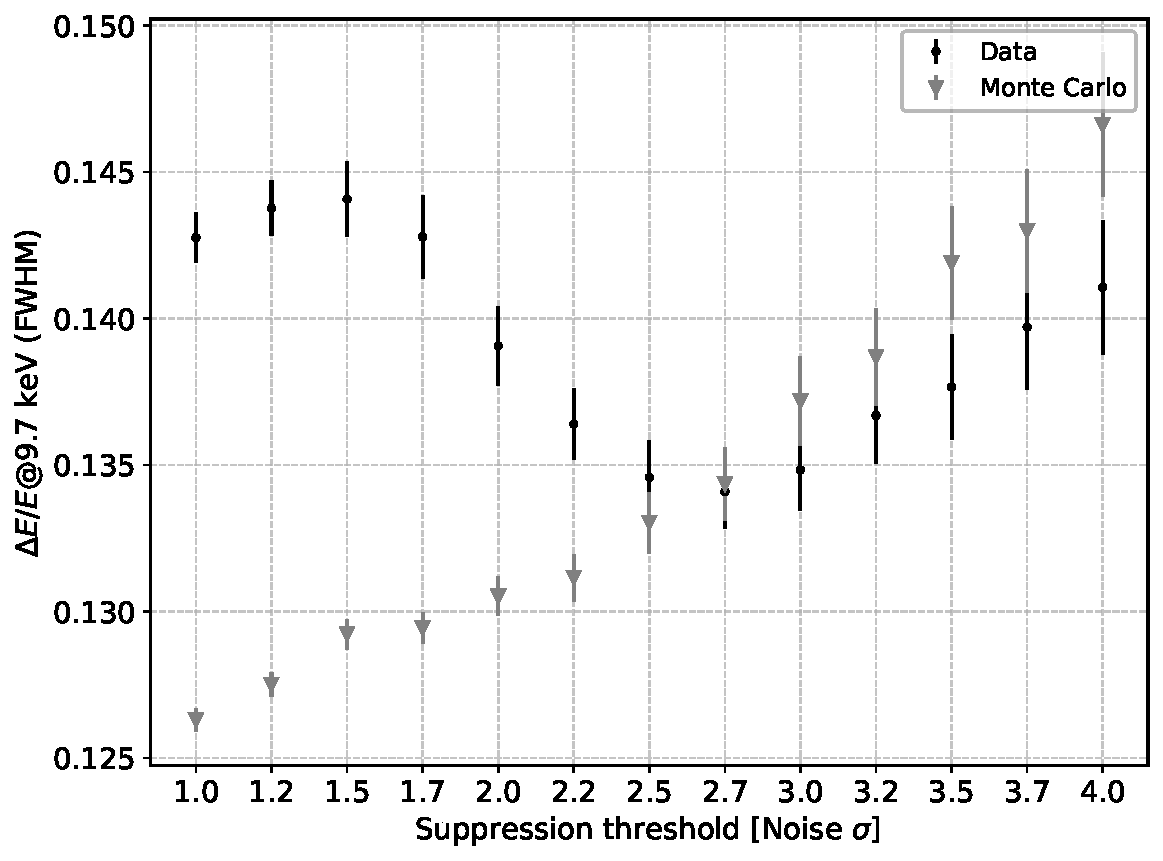
\includegraphics[width=0.49\linewidth]{figures/chapter4/results/zsup_dependence}
    \caption{Example of Au spectrum obtained from an X-ray tube  operated at 25 kV (left panel). The two dominant lines are gold fluorescence lines $L\alpha$ at 9.7 keV and $L\beta$ at 11.5 keV. The spectrum is obtained with a zero-suppression threshold of 2.5$\sigma$ of noise and shows all the events. The dependence of energy resolution on the threshold (right panel) shows that for laboratory data the best resolution is achieved at around 2.5--3.0$\sigma$, while for Monte Carlo simulations it is achieved with lower threshold values. The two dashed lines with the respective error bands show the energy resolution estimate with the MLE algorithm, which is independent from the suppression threshold.}
    \label{fig:spectrum_fit}
\end{figure}

Both laboratory and simulated datasets were also analyzed using the MLE algorithm. For experimental data, the MLE achieves an energy resolution slightly worse than the optimal value obtained with the suppression method. This discrepancy arises from the algorithm's calibration, which relies on Monte Carlo simulations: differences between the simulated and real detector response degrade the reconstruction accuracy. On the other hand, when applied directly to simulated data, the MLE reaches an energy resolution comparable to the best performance achieved by the suppression method. Further measurements are required to determine whether the higher complexity of the MLE algorithm is justified, given that the simpler suppression algorithm achieves the same or even better results on real data.

In conclusion, the current prototype is far from the design goal of 20\,$e^-$ ENC of noise per pixel, which can be achieved only with the ASIC that is currently being designed. At the moment, the single-pixel noise contribution is around 400\,eV. The results obtained with this prototype validate the reconstruction framework and demonstrate the effectiveness of both offline algorithms. Once the final low-noise front-end electronics is coupled to the active sensor, the energy resolution is expected to improve by a factor of 4--5, reaching the targeted $\sim$300\,eV FWHM at 10\,keV and enabling the separation of closely spaced fluorescence lines in applications such as XRD and astrophysical spectroscopy.

\subsection{Cluster size distribution}

\begin{figure}[!b]
\centering
	$\vcenter{\hbox{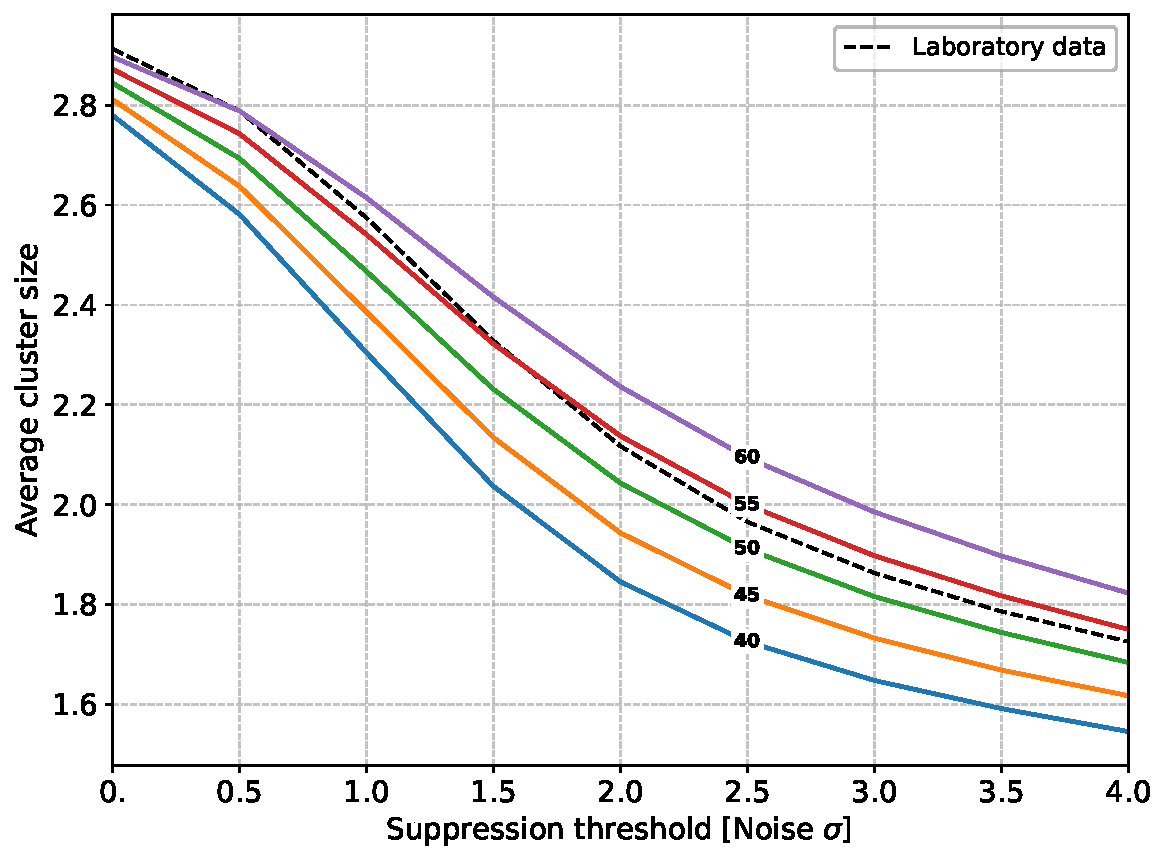
\includegraphics[width=0.55\linewidth]{figures/chapter4/results/cluster_size}}}$\hfill
    $\vcenter{\hbox{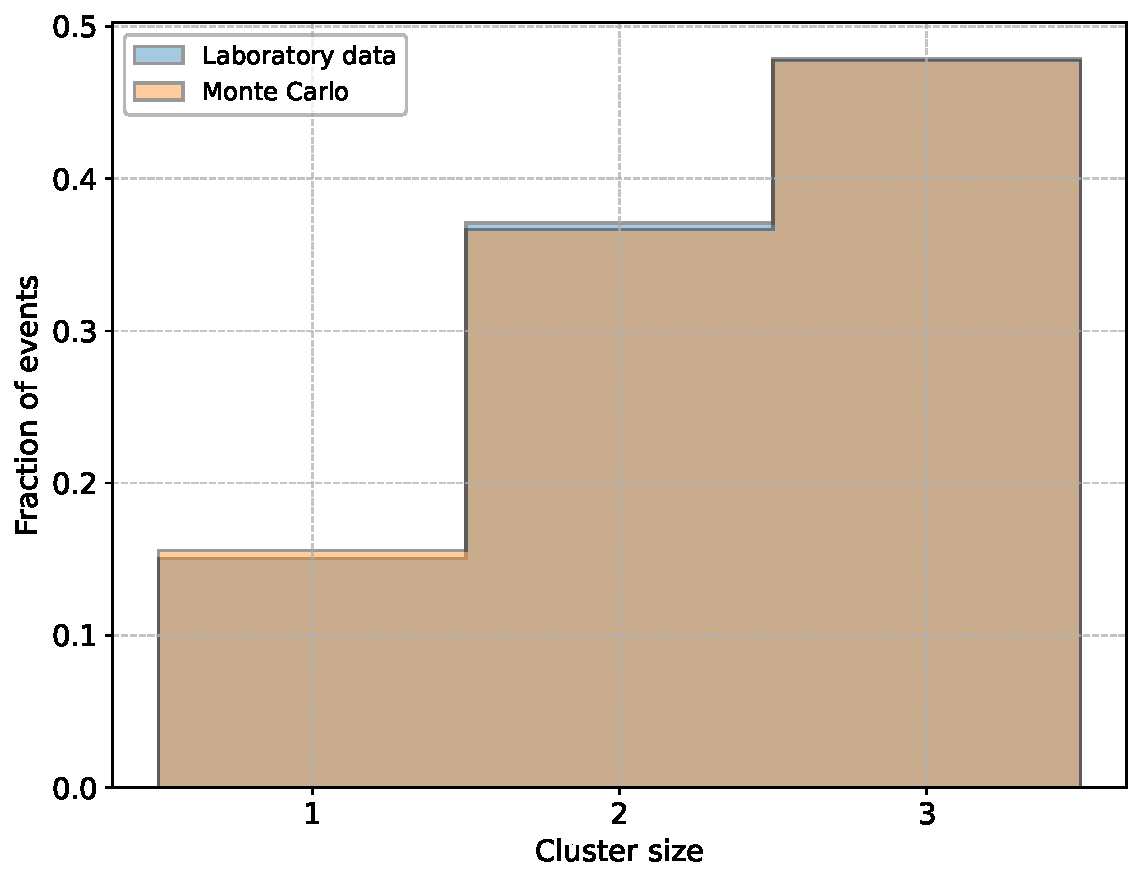
\includegraphics[width=0.45\linewidth]{figures/chapter4/results/cluster_size_hist}}}$
    	\caption{Average cluster size as a function of the zero-suppression threshold for laboratory data and Monte Carlo simulations generated with different diffusion coefficients ranging from 40 to 60 $\mu$m~cm$^{-0.5}$ (left panel). The experimental data points are best matched by the simulation with 55~$\mu$m~cm$^{-0.5}$. Normalized cluster size distribution for laboratory data compared to the Monte Carlo simulation with a diffusion coefficient of 55~$\mu$m~cm$^{-0.5}$, obtained with a zero-suppression threshold of 1.5\,$\sigma$ (right panel).}
\label{fig:cluster_size}
\end{figure}

In addition to comparing the spatial and energy resolutions between laboratory data and Monte Carlo simulations, another relevant quantity that can be evaluated is the cluster size. This metric depends primarily on the charge diffusion geometry and the pixel pitch. While the pixel pitch is precisely known, charge diffusion is harder to estimate accurately due to uncertainties in the diffusion coefficient. In fact, various physical effects, such as local electric field variations, doping non-uniformities, and temperature fluctuations, can introduce a significant uncertainty on its nominal value. Furthermore, pixel crosstalk acts as an additional charge-sharing mechanism, effectively spreading charge across adjacent pixels as if the diffusion coefficient were larger.

For this reason, the effective diffusion coefficient used in the Monte Carlo simulations is tuned by matching the laboratory data. Specifically, events are reconstructed with different zero-suppression thresholds, following the same procedure adopted for the energy reconstruction, to evaluate the average cluster size distribution. Multiple datasets matching the experimental source spectrum, noise, and gain are then simulated for different diffusion coefficients.

The comparison between experimental and simulated data is shown in Fig.~\ref{fig:cluster_size}. For the gold spectrum dataset used to evaluate the energy resolution, the diffusion coefficient that best describes the experimental data is found to be around $55\,\mu\text{m}\,\text{cm}^{-0.5}$. This agreement is confirmed by comparing the cluster size distributions, particularly at a threshold of $1.5\,\sigma$.

\section{Conclusions}
In summary, the characterization of the current ASIX prototypes has successfully validated both the proposed architecture and its dedicated simulation and analysis framework. By combining experimental measurements, using line pair phantoms for spatial resolution and fluorescence targets for spectroscopy, with Monte Carlo simulations, a complete data processing pipeline has been established and tested. This framework covers the entire analysis workflow: it starts from the fundamental calibration of detector non-uniformities, such as noise levels, baseline offsets, and normalized gain, and integrates these products into the event reconstruction process to improve the estimate of the photon energy and its sub-pixel incidence position.

Although the experimental spatial and energy resolutions are currently constrained by the high electronic noise of the XPOL-III readout chip, the implementation of advanced reconstruction algorithms confirms the validity of the underlying physical models. In particular, both the maximum likelihood estimator and the $\eta$ algorithms have demonstrated their superiority over simple charge barycentering, proving that exploiting the charge sharing geometry is the key to achieving sub-pixel spatial resolution. Furthermore, the agreement found between experimental data and simulations, such as in the matching of the cluster size distributions, proves the reliability of the current simulation software for these preliminary studies. However, since the current Monte Carlo framework is based on a simplified physical model, it will need to be upgraded by integrating a full Geant4 simulation to accurately account for all the relevant physical processes.

The integration of a new low-noise XPOL ASIC, with a target of less than $20\text{ e}^-$ ENC per pixel and the seven-pixel parallel readout logic, will finally overcome the current hardware limitations. In preparation for this upgrade, the analysis framework discussed in this work provides a validated environment, ready to be employed for the characterization of the final detector in the next development phases.

\chapter{$\mu$GPD}
\label{chap:chapter5}

In the context of X-ray polarimetry, the current Gas Pixel Detectors that are employed on board of IXPE do not match the requirements of the next generation of X-ray polarimeters, such as eXTP. The strictest requirements that have to be satisfied concern the ability to detect photons at a much higher rate than IXPE and to improve the detector stability over time.

The current GPDs employ a finely pixelated ASIC to reconstruct the two-dimensional photoelectron track produced by the absorption of a X-ray photon. This is at the basis of how a photoelectric polarimeter works, and thanks to 50 $\mu$m wide pixels a GPD can perform it with good accuracy, which is translated into a high polarization sensitivity.

As mentioned in Chap. \ref{chap:chapter3}, the main limitations of a GPD are the residual non-uniformities in the azimuthal response, which lead to the so-called spurious modulation, and rate-dependent gain variations. Both these problems can be attributed to the multiplication element of the GPD, the GEM.

The spurious modulation is caused by the manufacturing process of the GEM, where small shape variations between the holes induce a position-dependent systematic effect which is difficult to characterize and correct.

On the other hand, rate-dependent gain variations are attributed to the large dielectric surface inside a GEM hole, which leads to the trapping of part of the charge produced during the avalanche. The consequence of this dielectric charging phenomenon is a change in the configuration of the electric field inside the hole, which results in the decrease of the gain factor.

If the detector is constantly exposed to radiation, charges accumulate with time and the gain keeps varying until a saturation level that depends on the event rate, or more precisely on the incoming energy flux. This means that when switching observations between sources with different fluxes the gain is not stable until a new equilibrium level.

A new type of multiplication stage is under development to replace the GEM and overcome these limitations. The idea behind $\mu$GPD \cite{sgro2026} is to use a micro-gap-like \cite{angelini1993} structure built directly on top of the ASIC.

\section{Detector design}

$mu$GPD represents one of the possible successors of the current GPD generation. The basic working principles remain the same, that is a photoelectric polarimeter which employs a gas active volume to absorb X-ray photons and produce a photoelectron, which is emitted in a direction that depends on the photon polarization. The photoelectron track produced by primary ionization is used to measure the emission angle, and for this purpose the charges are multiplied and subsequently read by an ASIC which acts as collection anode.

The fundamental difference is in the multiplication stage, which in $\mu$GPD consists of structures deposited directly on top of the ASIC. A comparison between the current and one of the proposed designs is shown in Fig. \ref{fig:mugpd}.

The design and the idea behind these structures are similar to micro-gap chambers, which are based on two metal layers separated by a thin isolation layer. The upper-most layer is segmented in one-dimensional or two-dimensional structures only a few $\mu$m large an acts as the anode, while the bottom layer is usually a plane and acts as the catode

Applying a potential difference between the two electrodes generates a strong electric field in a small volume just above the anode. The primary ionizations electrons are drifted toward the anode, where they are accelerating by the electric field and produce an avalanche. The electrons are collected by the anode, while the ions are collected by the bottom layer cathode. An example of the avalanche process is shown in Fig. \ref{fig:avalanche}.

This design is a good candidate to solve the issues of the current generation of GPD. First, the deposition of the dielectric and the anode on top of the ASIC is made with photolitographic techniques, which allow to achieve sub-micron precision in the structure manufacturing. This way, gain non-uniformities across the sensor are strongly reduced. Furthermore, the surface of exposed dielectric is small and the amount of charge that can be accumulated is reduced, improving gain stability.

\begin{figure}[!t]
    \centering
    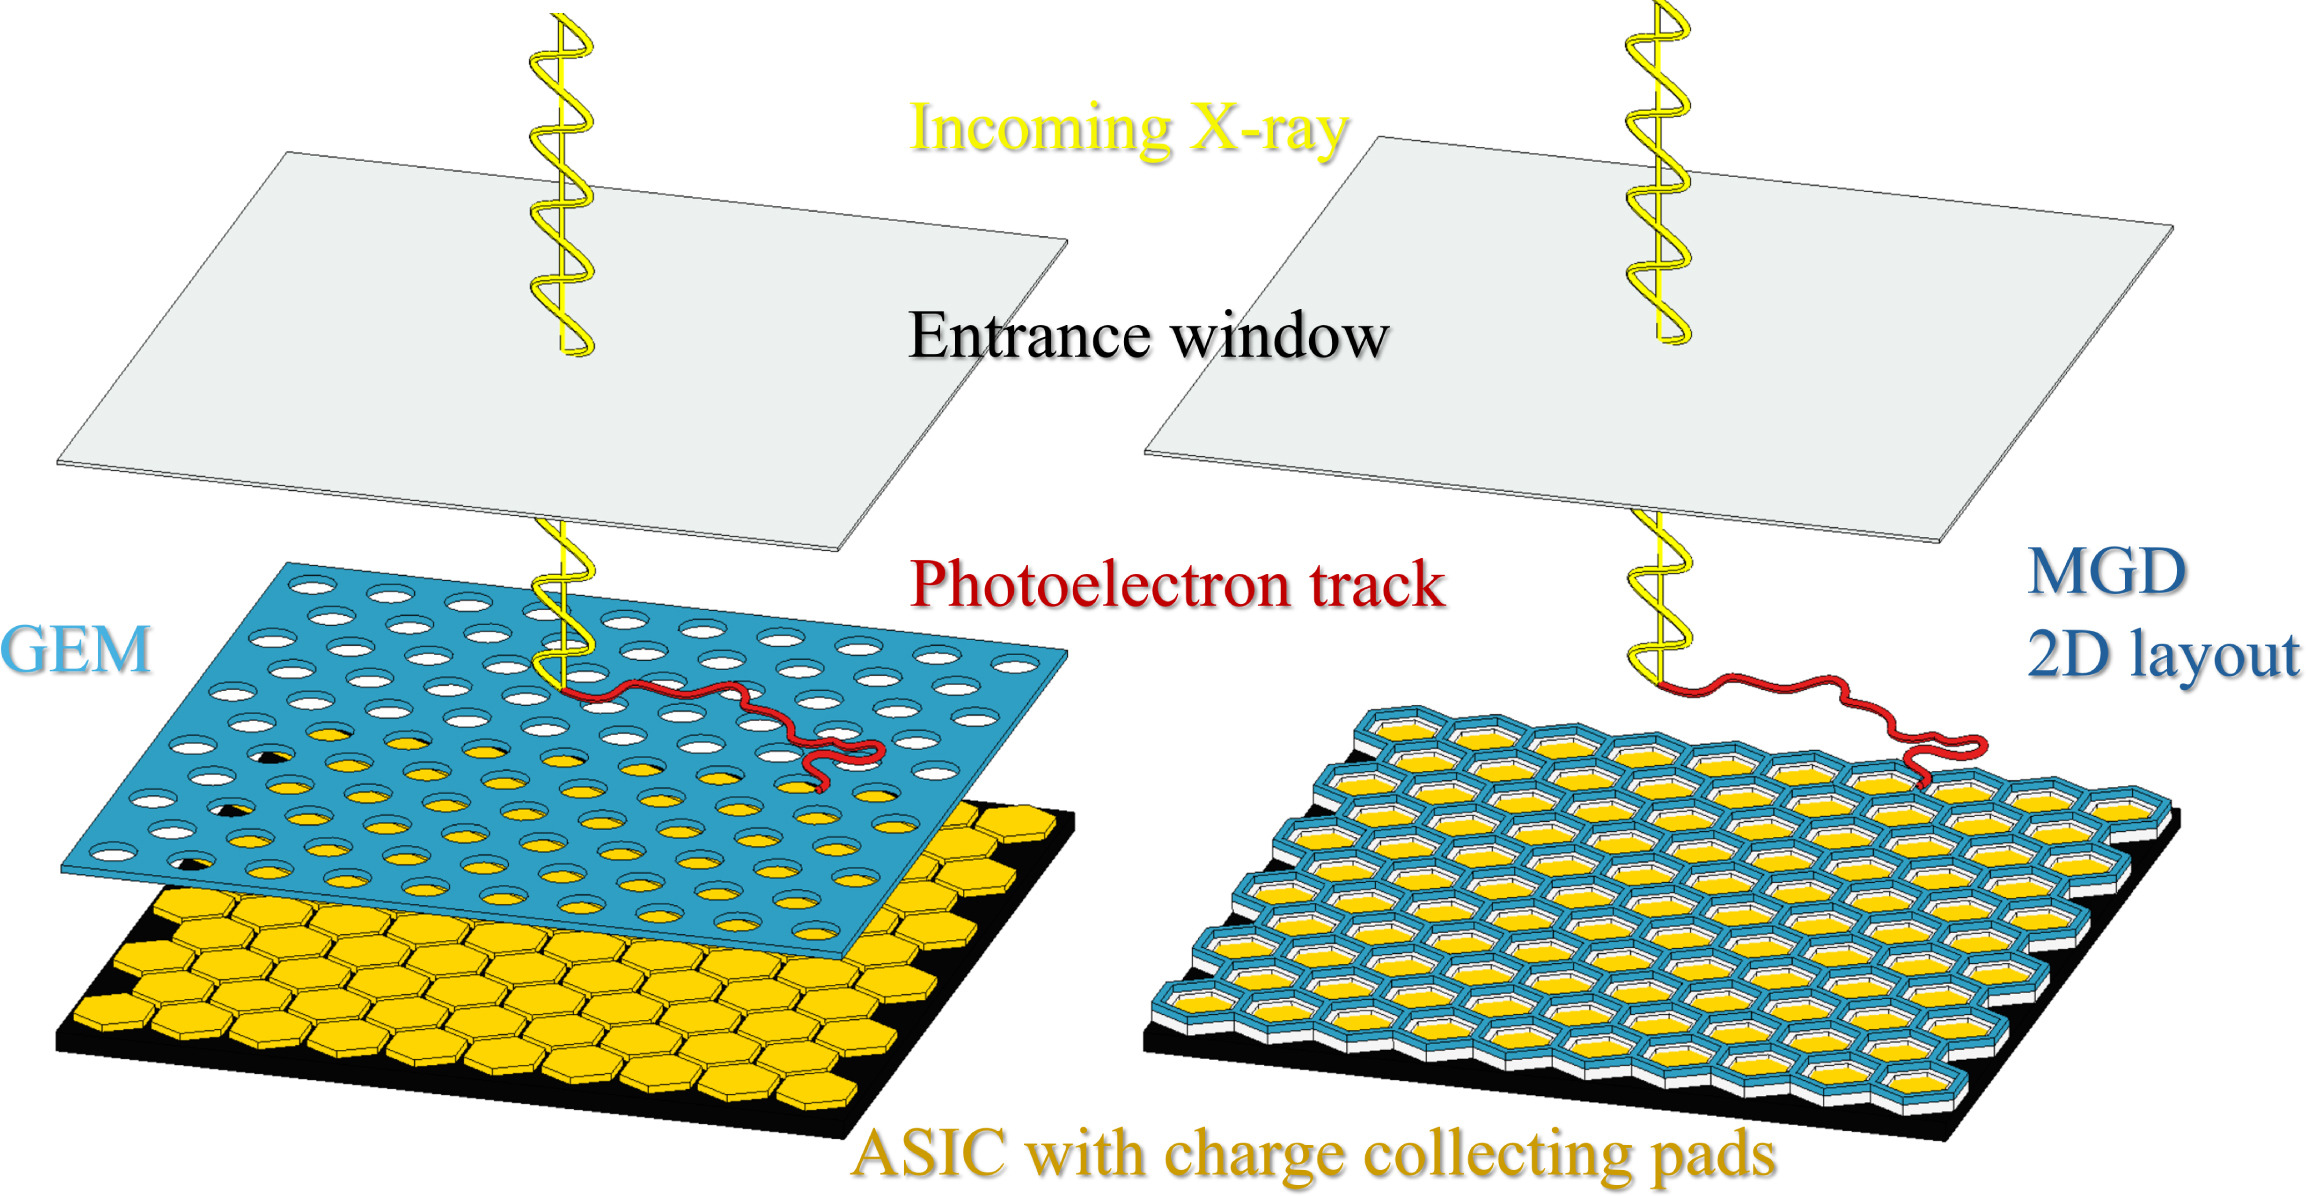
\includegraphics[width=0.7\linewidth]{figures/chapter5/mugpd}
    \caption{Comparison between the current GPD configuration (left panel) and the new proposed configuration with a hexagonal two-dimensional multiplication structure (right). X-rays are absorbed by the active gas volume and emit a photoelectron, which drifts toward the electron multiplier structure. In both cases the track shape is preserved by the multiplication structure. Image taken from \cite{sgro2026}.}
    \label{fig:mugpd}
\end{figure}


\begin{figure}[htpb]
    \centering
    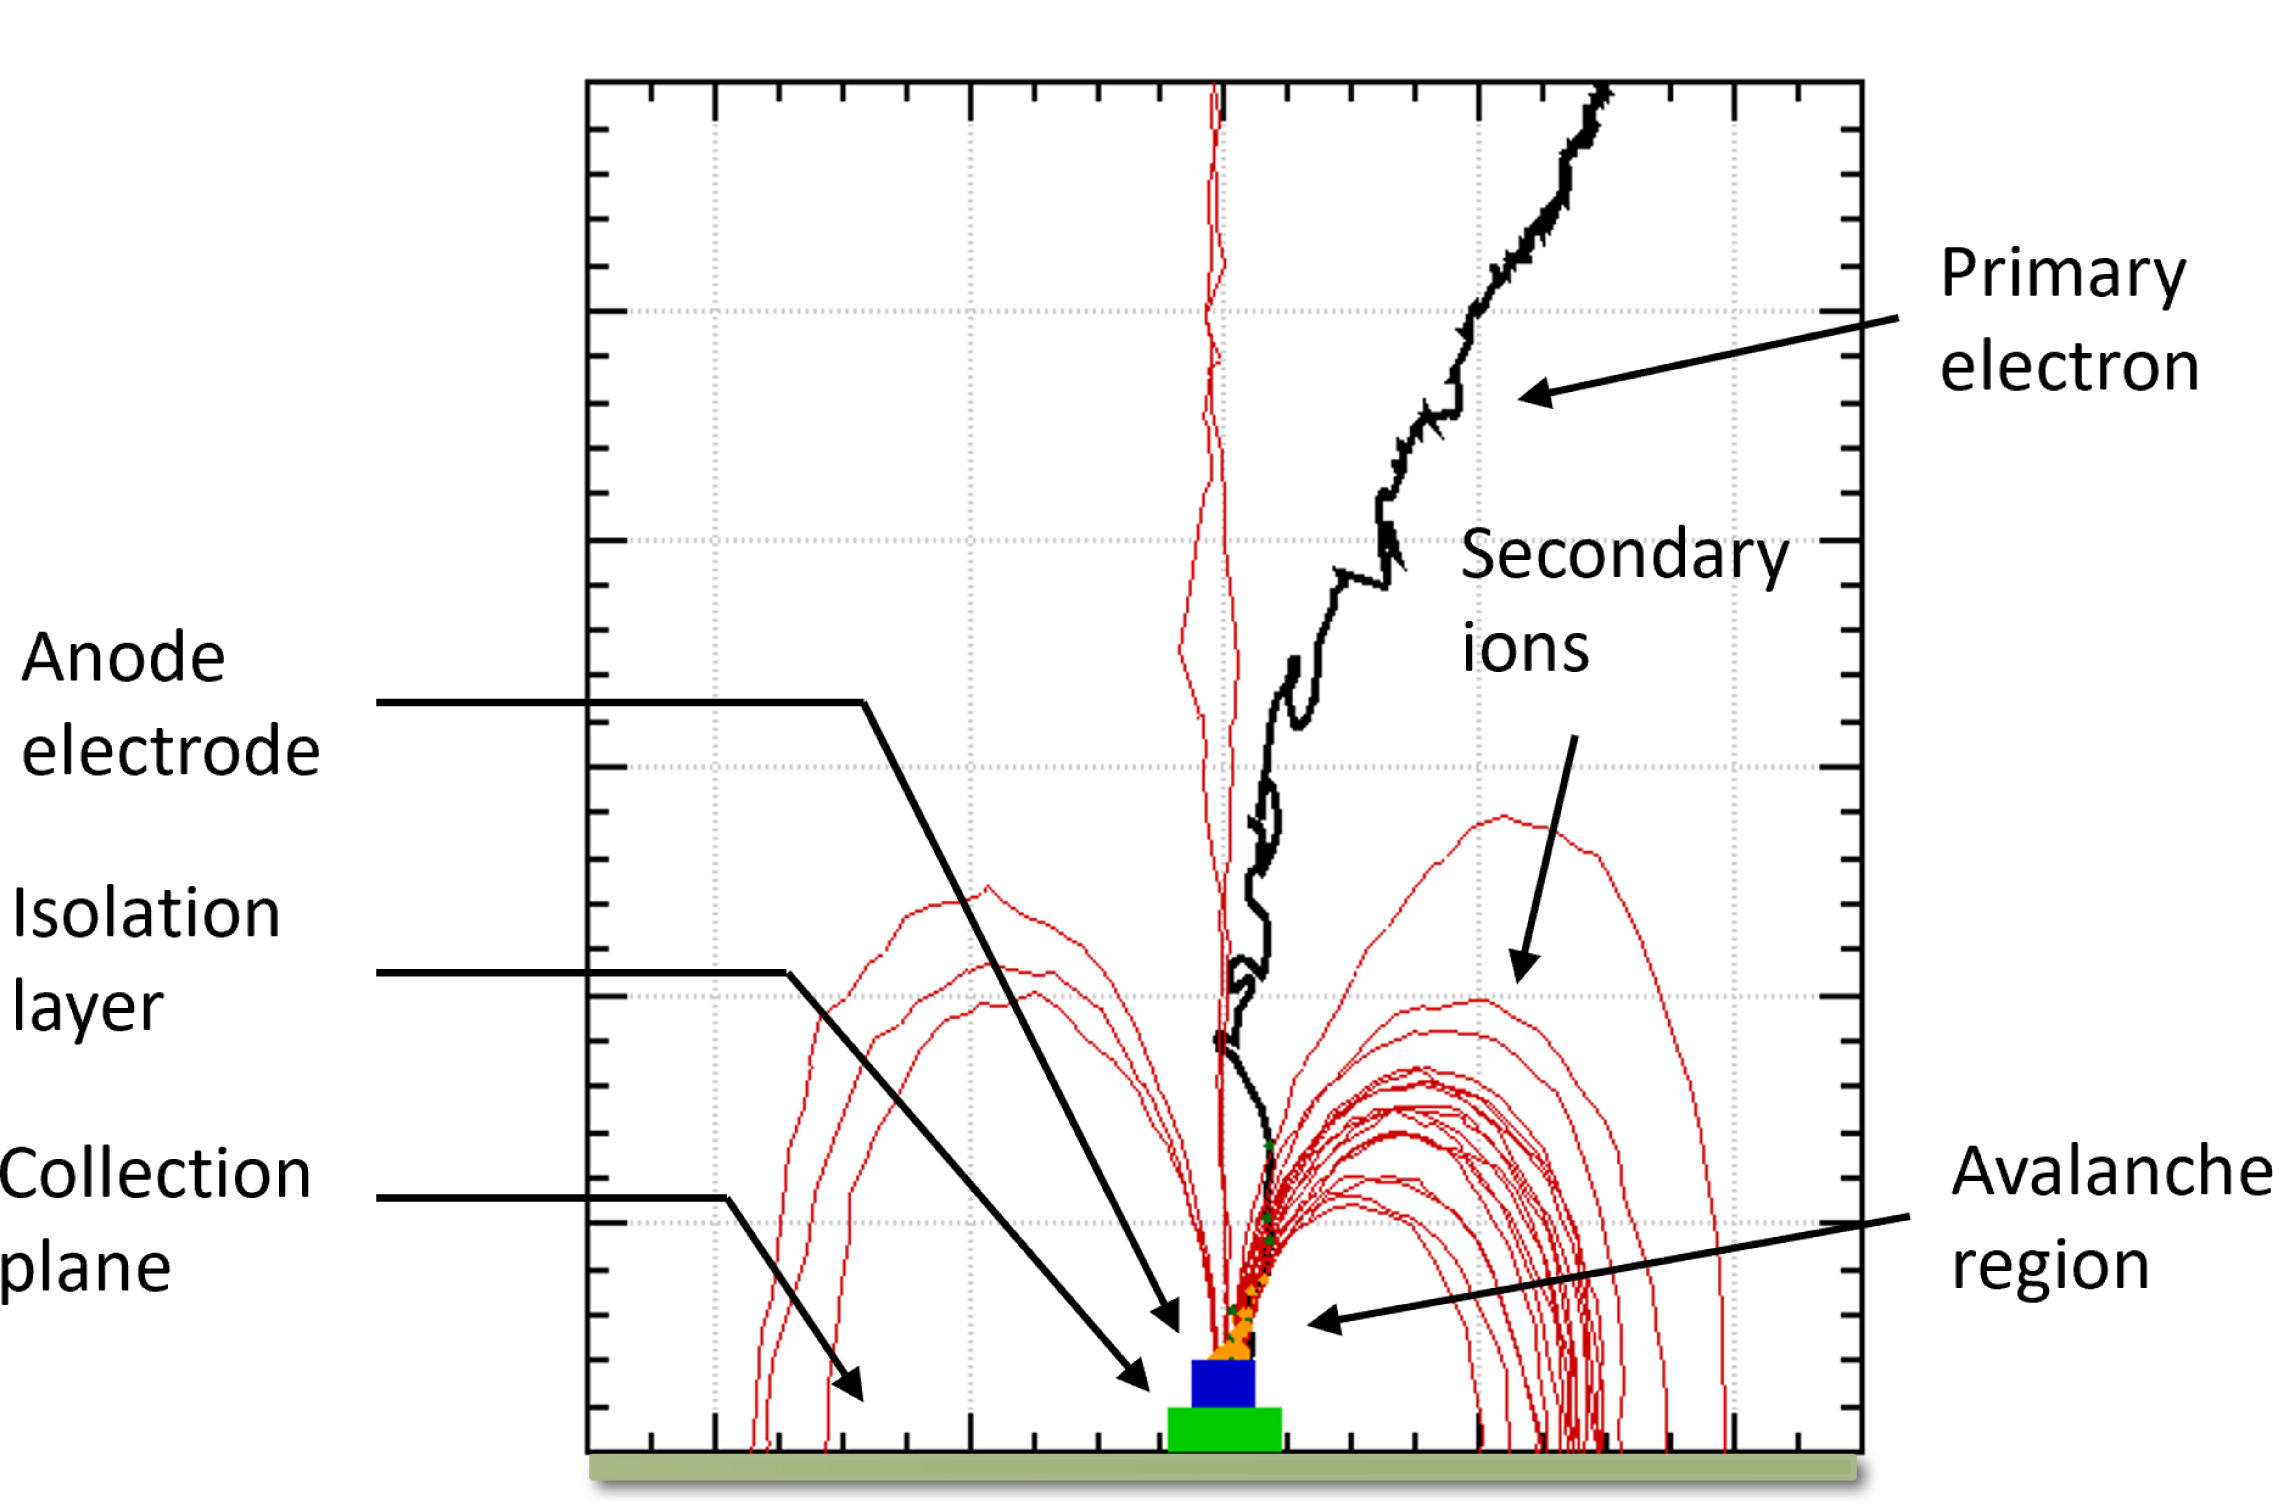
\includegraphics[width=0.6\linewidth]{figures/chapter5/avalanche}
    \caption{Schematic representation of how a micro-gap works. The avalanche is produced due to the strong electric field on top of the anode when a primary ionization electron is drifted toward it. Image taken from \cite{sgro2026}.}
    \label{fig:avalanche}
\end{figure}

At the current prototype stage, multiple anode geometries have been developed to understand which one provides the best detector performances while preserving the two-dimensional nature of the GPD. The proposed geometries are both one-dimensional and two-dimensional structures.

The one-dimensional structures consist of multiple parallel strips that run along  
the pixels. There are different designs currently under study, which vary in pitch and how they are aligned with respect to the pixels. In particular, one design has a pitch of 43.3 $\mu\text{m}$, with a strip aligned to the center of each pixel row. The other two designs have a larger pitch of 86.6 $\mu\text{m}$, where the strips are either aligned to the pixel centers or offset with respect to them.

For the two-dimensional structure the anode has the same shape of the hexagonal pixels, thus each pixel is surrounded by the anode line along its perimeter, as shown in Fig. \ref{fig:mugpd}.

In all the designs the the anode metal is made of aluminum, with a thickness of 2 $\mu$m and 5 $\mu$m wide. The isolation layer below the anode is built with high dielectric strength polyimide 2 $\mu$m thick and 13 $\mu$m wide.


\section{Prototype testing and performances}

At this stage of development, the primary objective is to verify whether these structures can withstand high voltages, which can cause breakdown sparks or leakage currents, and if they can achieve a gain comparable to that of a GEM at a sufficiently low voltage. Another relevant property that can be characterized is the energy resolution that the structures are able to achieve.

Various tests of the anode structures have been performed under different working conditions to verify their feasibility as multiplication stage in the next generation of GPD and to characterize their performances.

\subsection{Implementation on silicon wafer}
The first test that has been performed by building the structures directly on top of a high-resistivity silicon wafer, shown in Fig. \ref{fig:mugpd_wafer}, which acts as the collection layer. This first demonstrator serves to verify the possibility of creating these structures with photolitography processes on top of a substate similar to that of XPOL chips without compromising it.

To test the gain the wafer is placed inside a dedicated gas chamber. The metallic layer of a custom PCB is placed in contact with the back of the wafer to provide negative high voltage, while the anode structures are kept at 0 V.

\begin{figure}[!t]
    \centering
    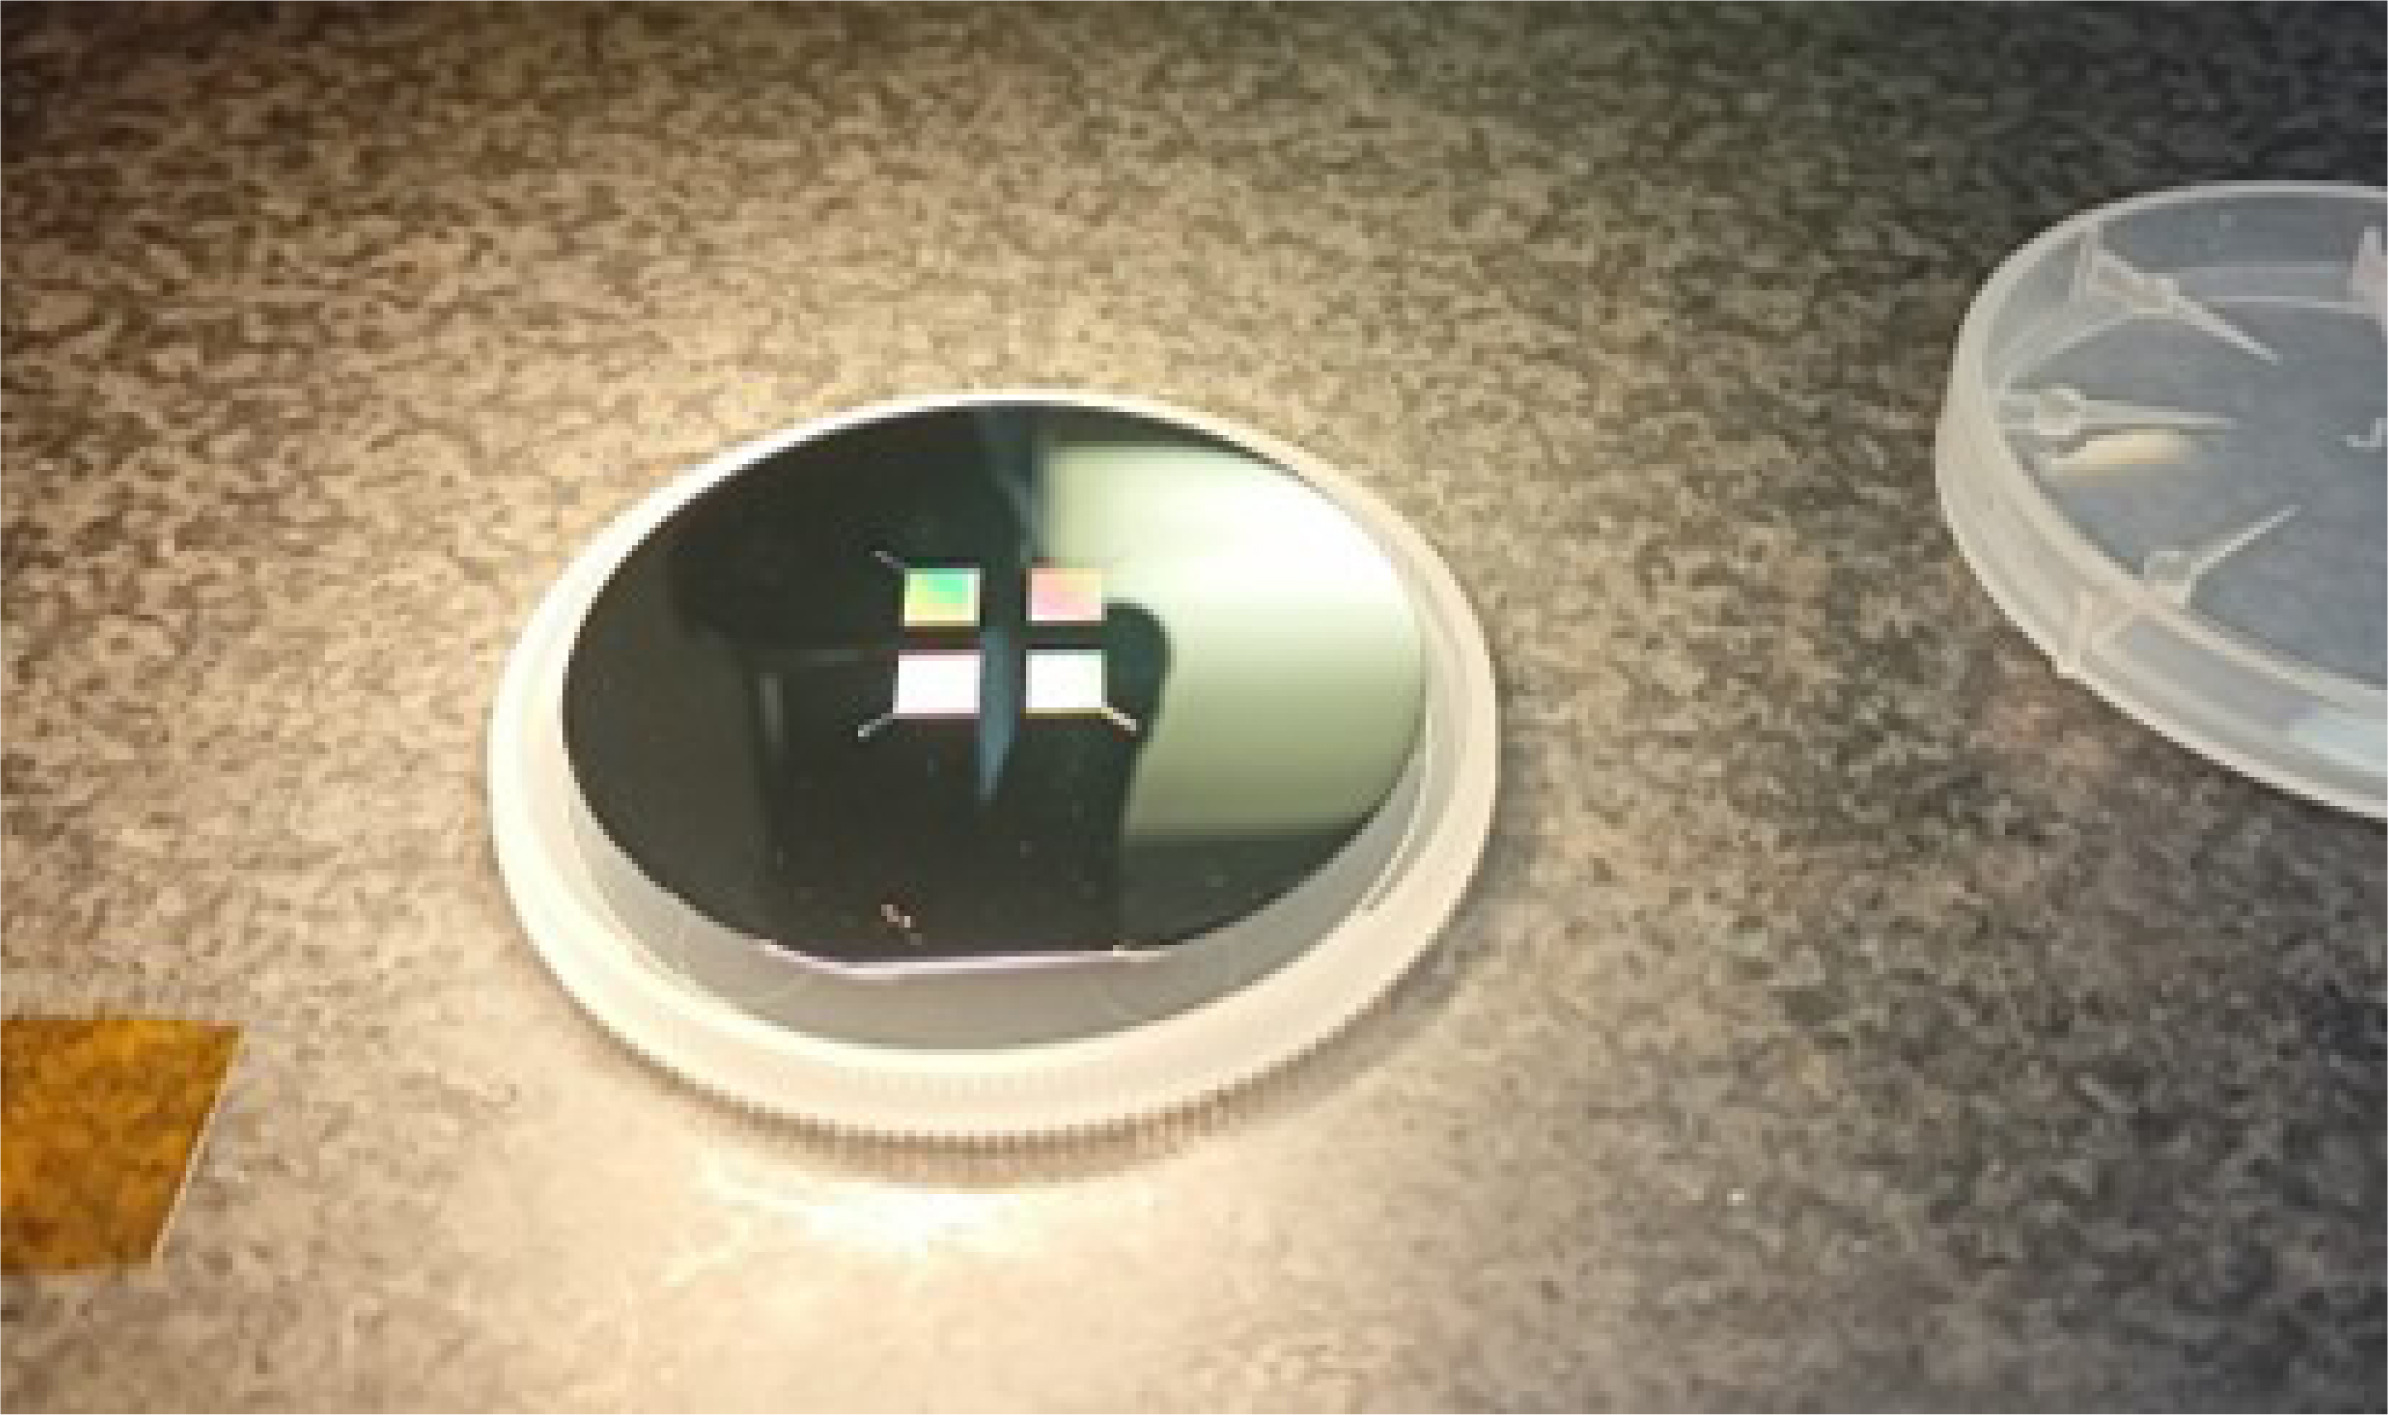
\includegraphics[width=0.6\linewidth]{figures/chapter5/mugpd_wafer}
    \caption{Picture of the silicon wafer with the four anode structures built on top. Image taken from \cite{sgro2026}.}
    \label{fig:wafer_performance}
\end{figure}


The anode structures are connected to a single channel spectroscopic amplifier which in turn is connected to a multichannel analyzer.

To define the absorption and drift region, a 1 cm thick spacer is placed on top of the structures. The entire assembly is placed in a closed box flushed with a mixture of Ar/Isobutane 80/20.

The structures are irradiated with a $^{55}$Fe source placed on top. $^{55}$Fe decays by electronic capture in $^{55}$Mn and it emits fluorescence radiation, with about 90\% probability of emitting $K\alpha$ at 5.9 keV and about 10\% probability of emitting $K\beta$ at 6.5 keV.

The focus of this initial test are the one-dimensional structures, comparing two designs with 43.3 $\mu$m and 86.6 $\mu$m pitch.

Before measuring the gain at different high voltage configurations, the electronic chain is calibrated with a charge injection circuit with a known input capacitance in order to convvert ADC values to charge.

For these preliminary tests the observed spectrum is fitted with a single Gaussian, even though the energy resolution is good enough to observe an asymmetry in the $K\alpha$ emission line due to the presence of the $K\beta$ line. The mean value of the best-fit Gaussian is used to estimate the gain, while the FWHM is used to estimated the energy resolution.

The dependence of gain and energy resolution as a function of the voltage difference of the gap is shown in Fig. \ref{fig:wafer_performance}. For the gain the exponential behaviour described in Eq. \ref{eq:exp_gain} is clearly visible. For both structures a gain of a few hundreds is achievable with voltages below 400 V, of the same magnitude of the GEM gain in GPDs, which is about 200.

It is also possible to observe that in the volateges range under test, energy resolution improves with higher gain. The best energy resolution is achieved by the 86.6 $\mu$m design, which is also the design that can reach a higher gain at lower voltages with respect to the 43.3 $\mu$m design.

\begin{figure}[htpb]
    \centering
    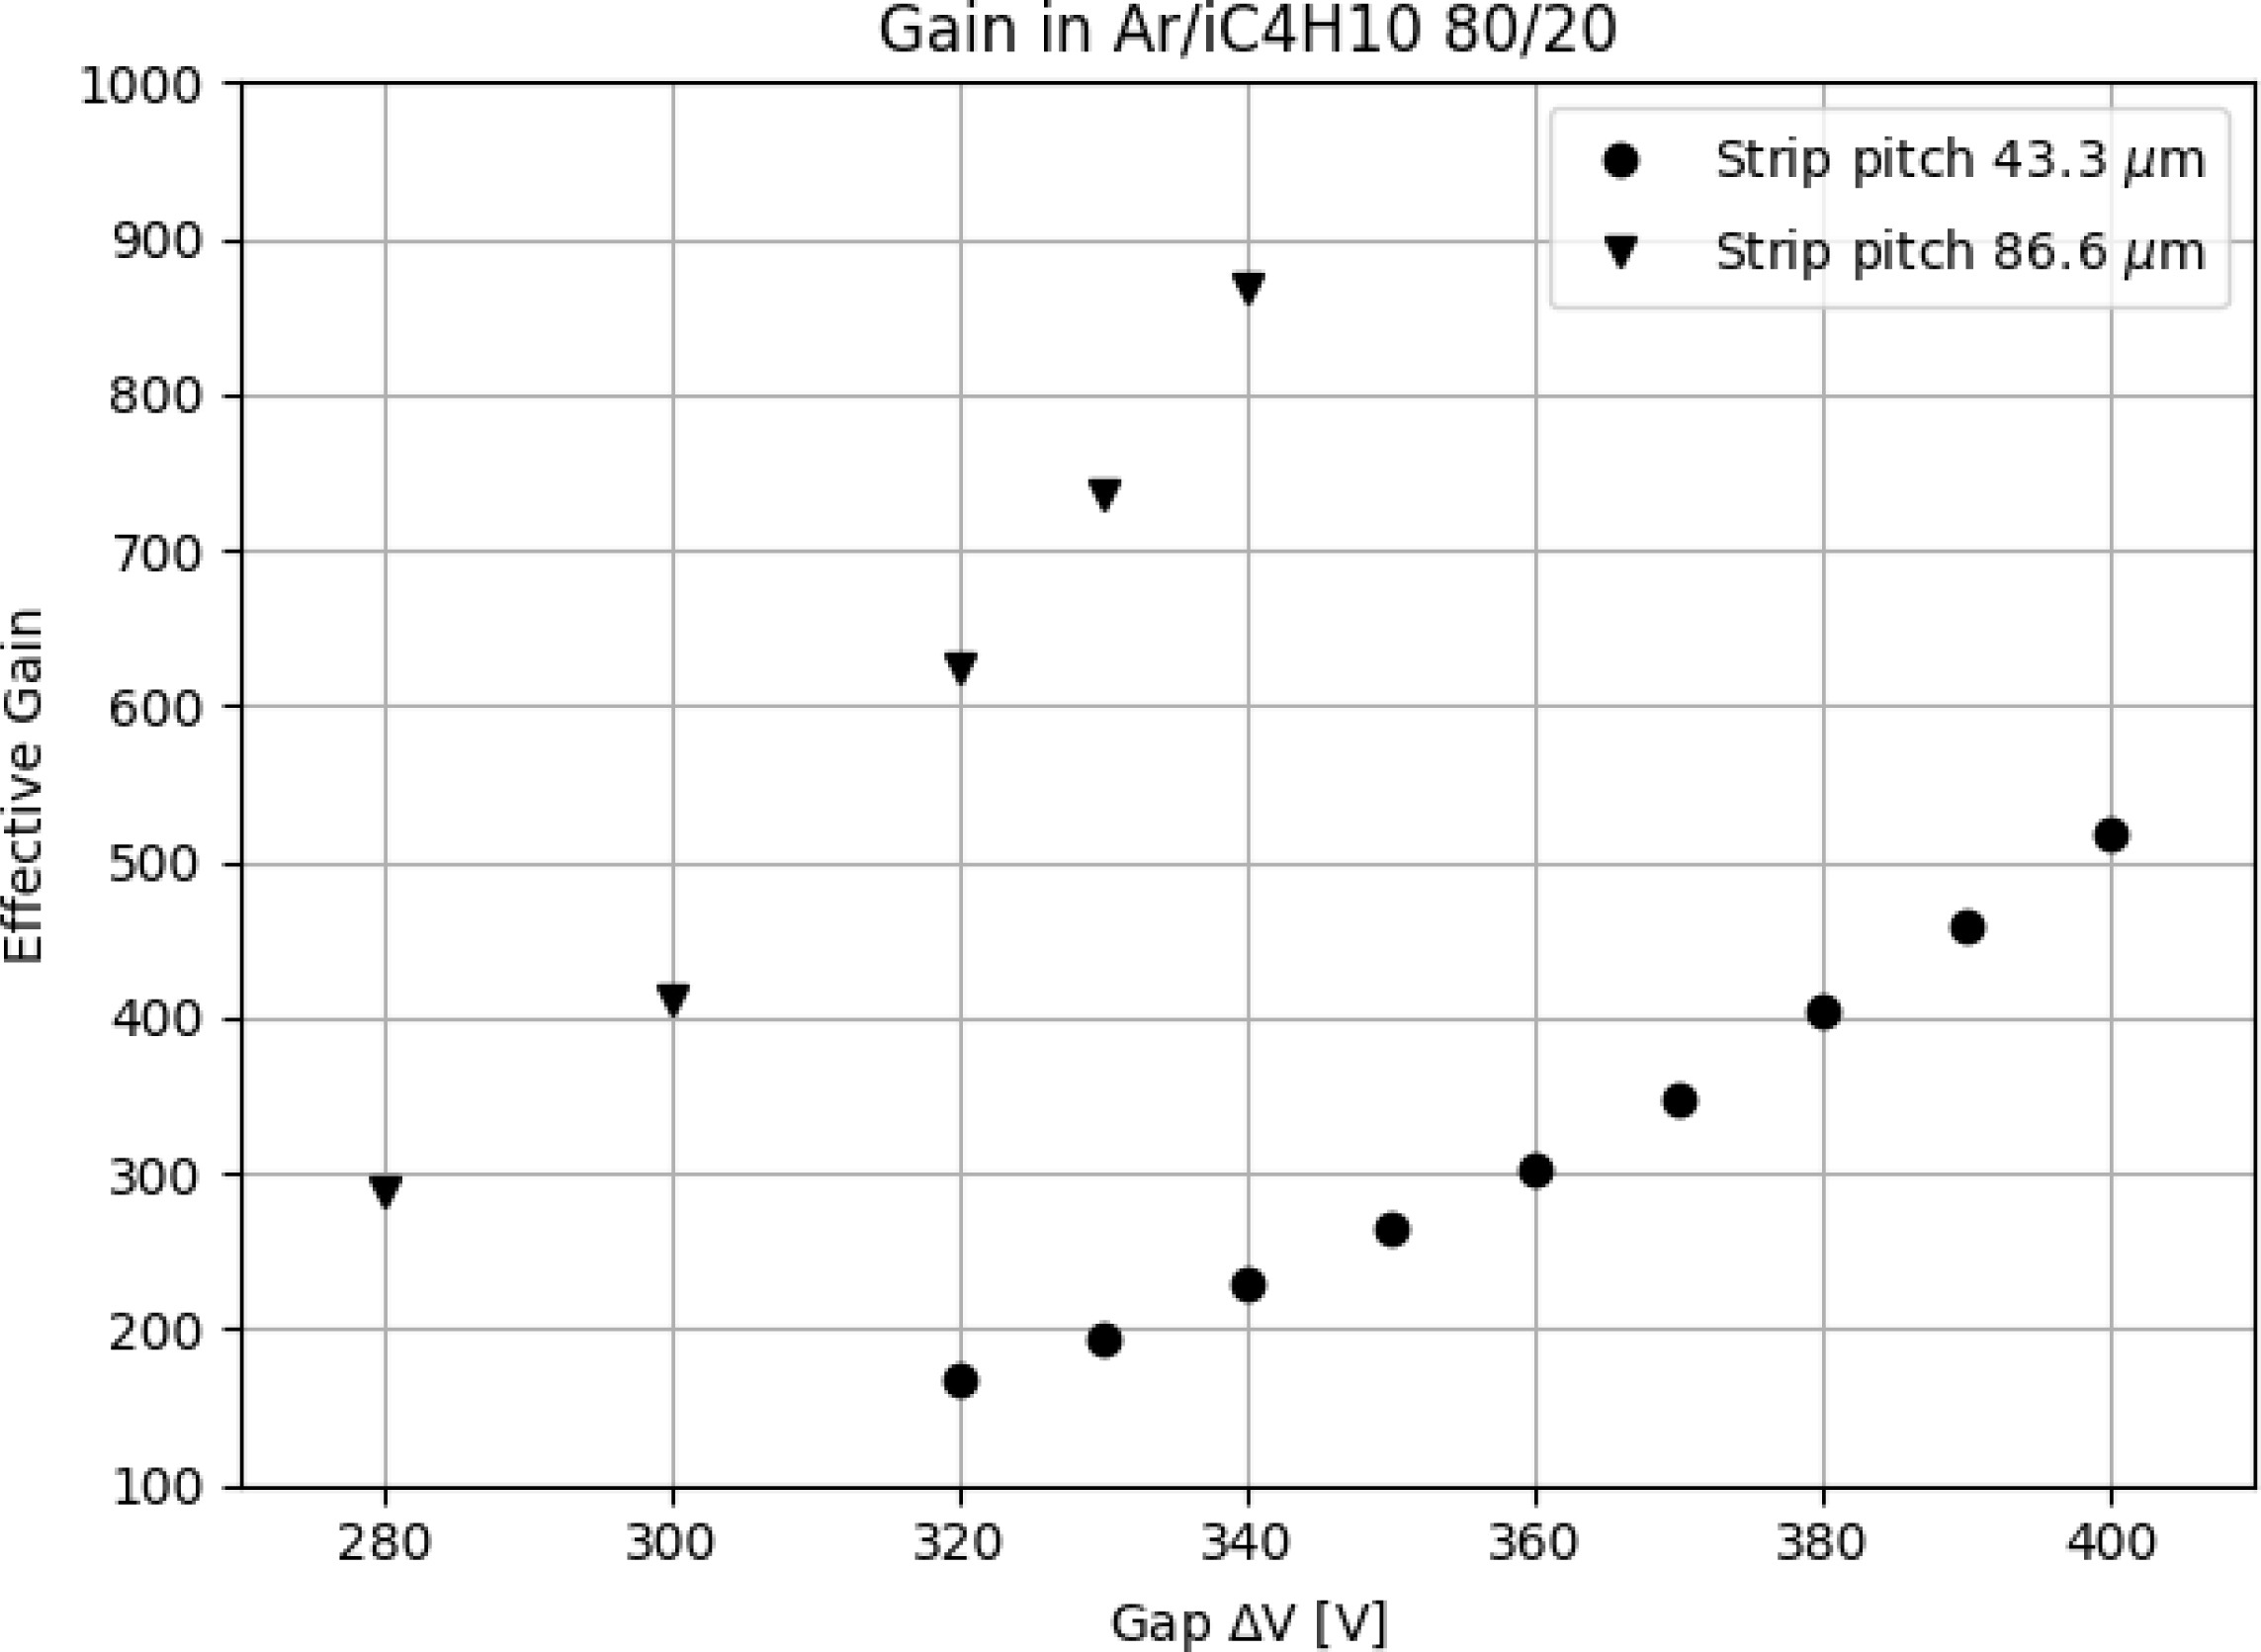
\includegraphics[width=0.49\linewidth]{figures/chapter5/gain_wafer}
        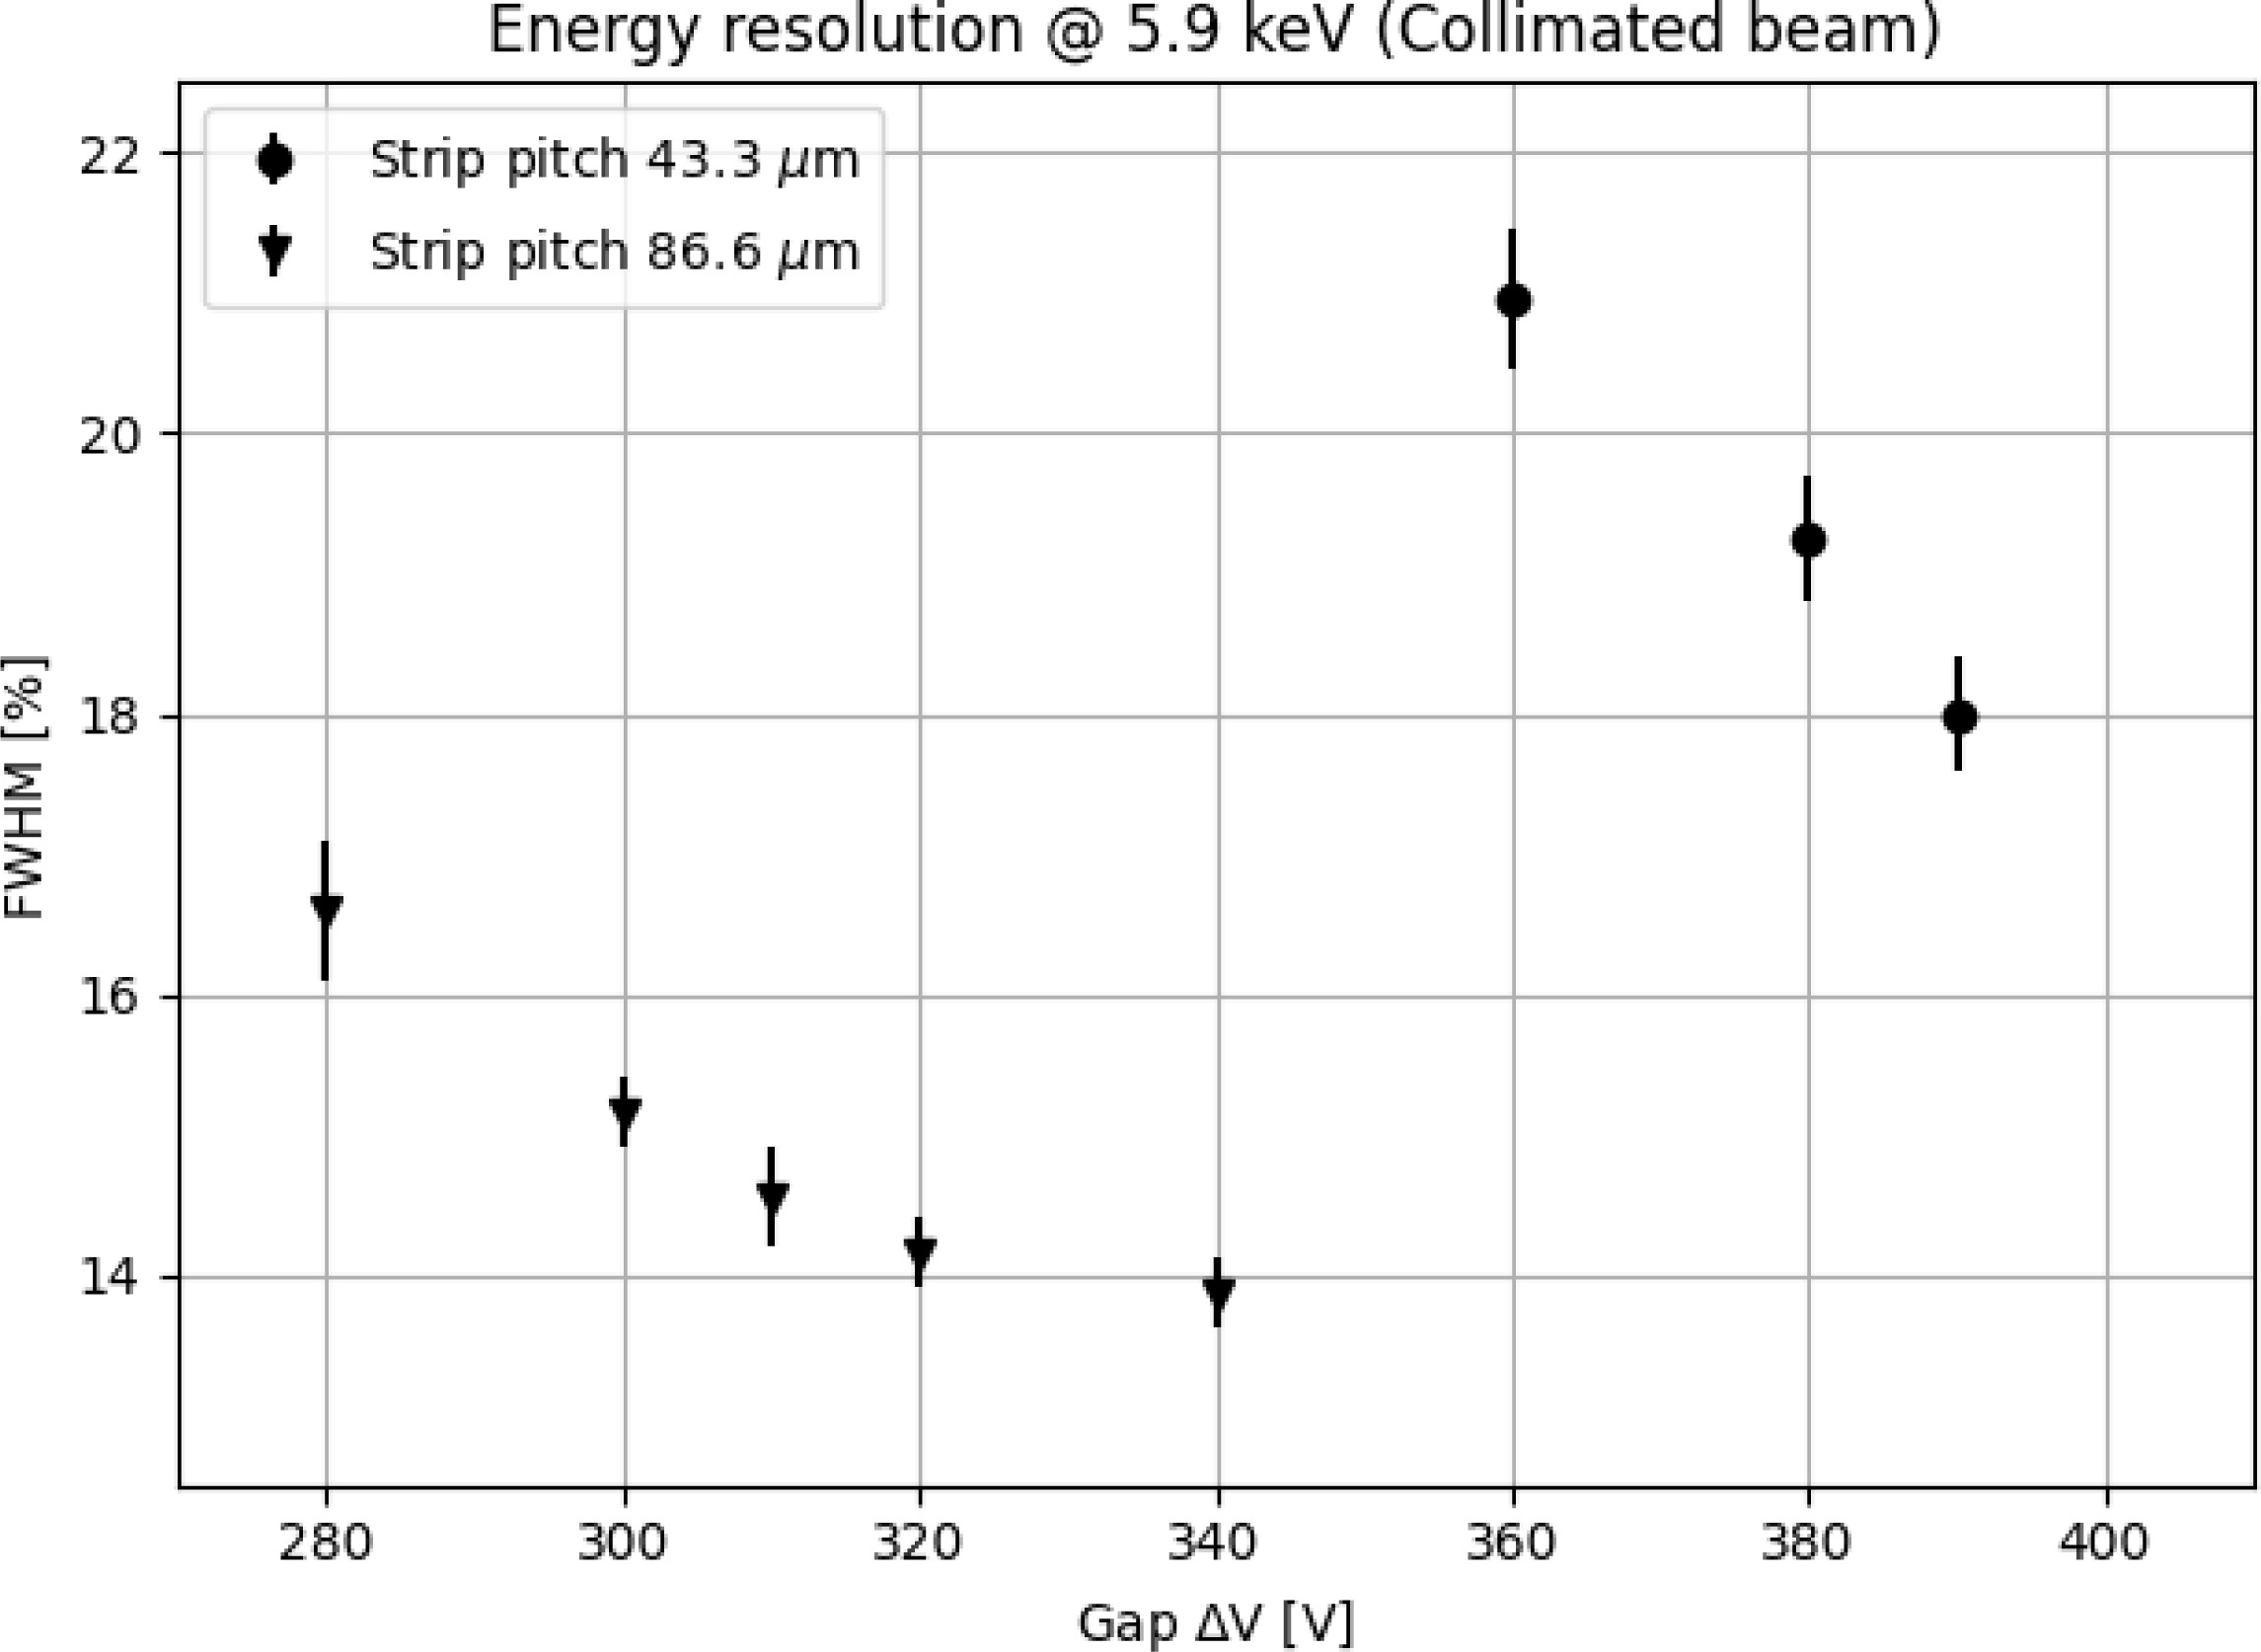
\includegraphics[width=0.49\linewidth]{figures/chapter5/resolution_wafer}
    \caption{Effective gain (left panel) and energy resolution (right panel) as a function of the anode-cathode voltage for one-dimensional structures with 43.3 $\mu$m and 86.6 $\mu$m pitch. Images taken from \cite{sgro2026}.}
    \label{fig:wafer_performance}
\end{figure}

These first results prove that these structures built directly and monolithically on top of a XPOL-like chip can operate as multiplication stage.


\subsection{Integration on XPOL ASICs}
After proving that the structures can work on top of a chip, the successive step is to test prototypes build directly on top of pre-existing chips to see if the expectations are confirmed.

The four designs described above are fabricated on top of an XPOL chip, dividing the active area into four different regions of $5 \times 5$ mm$^2$, one for each design. Fig. \ref{fig:mugpd_chip} shows a picture of a chip with the four different multiplication stages built on top of it. 

In this configuration the collection plane is represented by the pixels top metal electrode. An important thing that must be noted is that the current chips are designed to collect electrons, not ions, thus they are not able to read the signal produced by the avalanche generated by the micro-gaps.













% Add the bibliography 
\nocite{*}
\printbibliography[heading=bibintoc]

\end{document}